\documentclass[a4paper,oneside]{memoir}
\usepackage{noweb}
\noweboptions{breakcode,longchunks,longxref}

\usepackage[hyphens]{url}
\usepackage[colorlinks]{hyperref}
\usepackage{authblk}

% Things to be included before \begin{document}, e.g. signature matrix, changelog, etc.

% probably always Coordinator for DPPS reports
\preparer{Natthan Pigoux}{LUPM}

\reviewer{Luisa Arrabito}{LUPM}

\approver{Mieke Bouwhuis}{CTAO}

% license / Copy Right
\setcopyright{\copyright{} CTAO / LUPM \the\year}
\licence{\ccBySaNc}

% contributors list on second page, can be as many people as needed
\author{\ApplicationAuthor{}}{\ApplicationAuthorOrganization{}}{All Chapters}


\title{%
  A LADOK3 Python API
}
\author{%
  Alexander Baltatzis,
  Daniel Bosk,
  Gerald Q.\ \enquote{Chip} Maguire Jr.
}
\affil{%
  KTH EECS\\
  \texttt{\{alba,dbosk,maguire\}@kth.se}
}

\begin{document}
\frontmatter
\maketitle

\vspace*{\fill}
\VerbatimInput{../LICENSE}
\clearpage

\begin{abstract}
  We provide a Python wrapper for the LADOK3 REST API\@.
This wrapper provide a useful object-oriented framework for working with LADOK 
and direct API calls that return the unprocessed JSON data directly from 
LADOK\@.

We also provide a command-line interface (CLI) for the library.
We then construct some useful (shell) scripts using this CLI\@.
These scripts automates the reporting of results from Canvas to LADOK\@.

\end{abstract}
\clearpage

\tableofcontents*
\clearpage

\mainmatter
\chapter{Introduction}

LADOK (abbreviation of \foreignlanguage{swedish}{Lokalt Adb–baserat 
DOKumentationssystem}, in Swedish) is the national documentation system for 
higher education in Sweden.
This is the documented source code of \texttt{ladok3}, a LADOK3 API wrapper for 
Python.

The \texttt{ladok3} library provides a non-GUI application (a command-line 
interface, CLI) that, similar to access via a web browser, only provides the 
user with access to the LADOK data and functionality that they would actually 
have based on their specific user permissions in LADOK.
It can be seem as a very streamlined web browser just for LADOK's web 
interface.
While the library exploits caching to reduce the load on the LADOK server, this 
represents a subset of the information that would otherwise be obtained via
LADOK's web GUI export functions.

You can install the \texttt{ladok3} package by running
\begin{minted}{bash}
python3 -m pip install ladok3 # to use it in Python, or
pipx install ladok3           # to just use the CLI
\end{minted}
in the terminal.

Then you can use the CLI by running \mintinline{bash}{ladok} in the terminal.
The command has built-in help, simply run \mintinline{bash}{ladok -h} to see 
the available commands.
However, the first thing you want to run after installing the package is
\begin{minted}[firstnumber=last]{bash}
ladok login
\end{minted}
This will set up your credentials for the CLI.
However, if you want to use the library in a script, you can read
\begin{minted}[firstnumber=last]{bash}
ladok login -h
\end{minted}
for alternative ways of providing your credentials.

For use in Python scripts,
we provide the main class \texttt{LadokSession} (\cref{LadokSession}).
The \texttt{LadokSession} class acts like \enquote{factories} and will return 
objects representing various LADOK data.
These data objects' classes inherit the \texttt{LadokData} (\cref{LadokData}) 
and \texttt{LadokRemoteData} (\cref{LadokRemoteData}) classes.
Data of the type \texttt{LadokData} is not expected to change, unlike 
\texttt{LadokRemoteData}, which is.
Objects of type \texttt{LadokRemoteData} know how to update themselves, \ie fetch 
and refresh their data from LADOK.
When relevant they can also write data to LADOK, \ie update entries such as 
results.

One design criteria is to improve performance.
We do this by caching all factory methods of any \texttt{LadokSession}.
The \texttt{LadokSession} itself is also designed to be cacheable: if the session to 
LADOK expires, it will automatically reauthenticate to establish a new session.

You can find a quick reference by running
\begin{minted}[firstnumber=last]{bash}
pydoc ladok3 # doesn't work if installed with pipx
\end{minted}



\part{Example applications}

\chapter{Transfer results from Canvas to LADOK}\label{SomeScripts}

\input{../src/ladok3/scripts.tex}

\chapter{Transfer results from Canvas to LADOK in Python}

Here we provide an example program~\texttt{canvas2ladok.py} which exports 
results from Canvas to LADOK for the introductory programming course~prgi 
(DD1315).

However, a better way to do this is by using the CLI
(see \cref{SomeScripts} for an even better version):
\begin{minted}{bash}
#!/bin/bash

. ${HOME}/.profile

year=22
courses="DD13(10HT${year}|17HT${year})"
components="(LAB[123]|MAT1|KAL1)"

canvaslms results -c "$courses" -A "$components" \
| sed -E "s/ ?[HV]T[0-9]{2}( \(.*\))?//" \
| ladok report -fv
\end{minted}

But now we'll have a look at how we can do this (well, a simpler version) in 
Python.


\input{../examples/canvas2ladok.tex}


\part{The command-line interface}

\chapter{The base interface}

\input{../src/ladok3/cli.tex}

\chapter{The \texttt{course} command}

\chapter{Data}
\label{s:gui.data}

The GUI provides several windows for viewing and editing data arrays. This chapter assumes you are
familiar with \tao data nomenclature as discussed in the \vn{Data} chapter of the \tao manual.

%-----------------------------------------------------------------
\section{Viewing Data}
\label{s:gui.data.view}

\begin{figure}
\centering
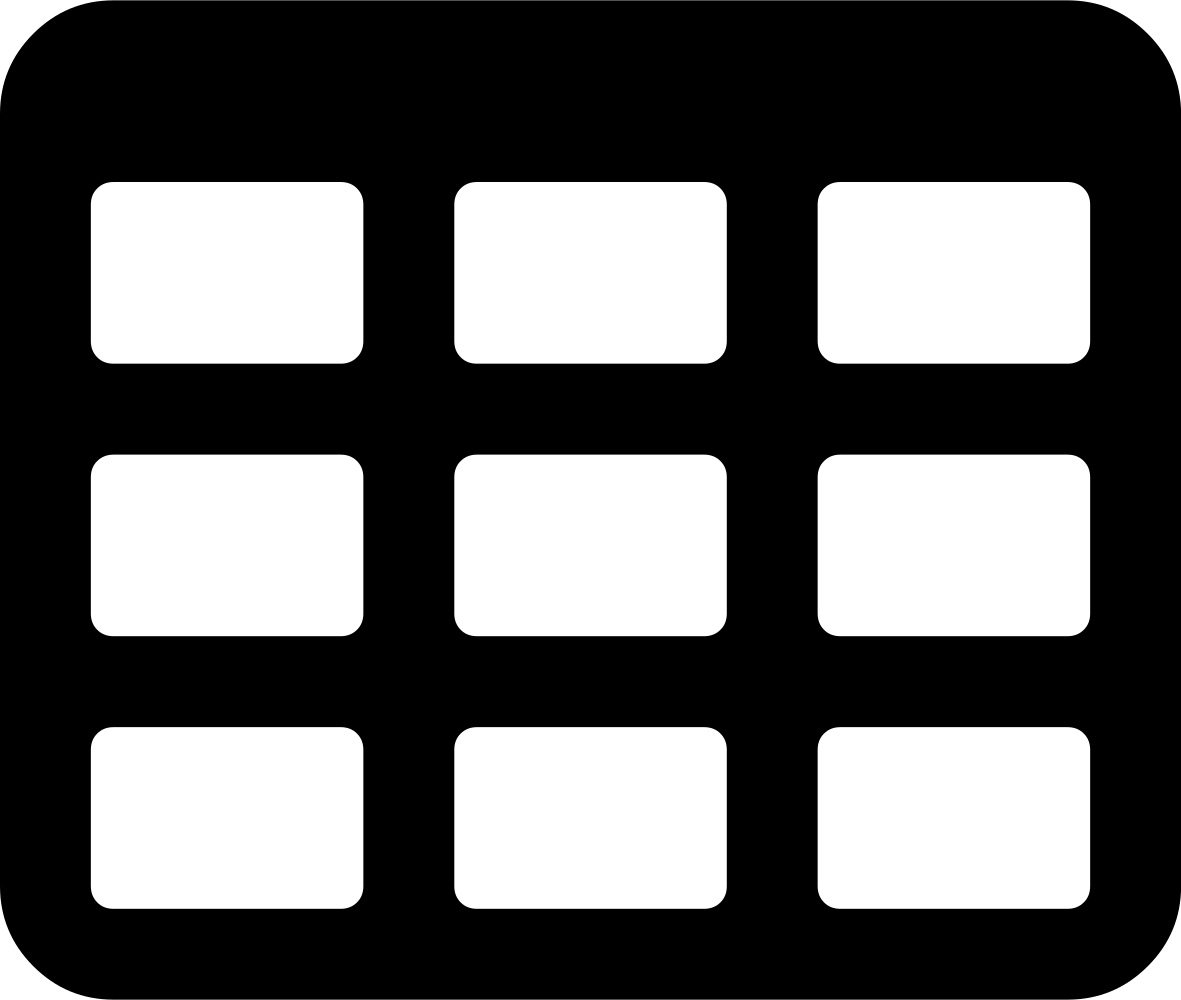
\includegraphics[width=12cm]{figures/view_data.pdf}
\caption[The GUI's data viewing windows.]{The GUI's data viewing windows.
Top left: the Tao root window and the menu shortcut for viewing data.
Top middle: The d2_data_array window, which list the currently defined d2_data_arrays for each universe.
This window also includes links to view and edit (see section \ref{s:gui.data.edit}) existing d1_data_arrays.
Bottom left: The d1_data_array window (in this case for orbit.x), showing all of the datums in the array orbit.x.
Bottom right: The individual datum window (in this case for orbit.x[34]) displaying detailed datum properties and allowing the user to edit some of these properties.
Top right: The bulk edit window (in this case for orbit.x) providing controls to quickly edit a few key properties for multiple datums in a d1_data_array.}
\label{fig:gui.data.view}
\end{figure}

Figure \ref{fig:gui.data.view} shows the various windows that the GUI provides for viewing data and making minor changes to data arrays.
The d2_data_array window (top middle in Figure \ref{fig:gui.data.view}) displays all data arrays for a given universe.
To view any existing d1_data_array, click on its "View" button.
This window also provides the ability to edit any existing data array in detail (see Section \ref{s:gui.data.edit}), as well as functionality for writing existing data to a namelist (see Section \ref{s:gui.namelist}).

The d1_data_array window (bottom left in Figure \ref{fig:gui.data.view}) allows the user to view an existing d1_data_array.
This window displays important properties of each datum in the array, such as element name, meas, model, and design values, and weight, in a scrollable table.
To view a datum in detail, double click on its row in the d1_data_array window.
This will open the individual datum window for that datum, displaying all of its properties and allowing some of them to be editted.

The d1_data_array window also allows the user to edit a few key properties of the datums in the array all at once using the bulk settings window (top right in Figure \ref{fig:gui.data.view}).
This window is accessed by clicking on the "Bulk fill" button in the d1_data_array window.
From here, the meas_value, good_user, and weight settings for the datums in the array can be edited in bulk.
Changes may be applied to every datum in the array, or to only a specific range of datums using the range specifier.
Once the desired settings have been specified, clicking the "Fill and apply" button will edit the d1_data_array as necessary, and changes will be reflected in the d1_data_array window.

%-----------------------------------------------------------------
\section{Creating and Editing Data}
\label{s:gui.data.edit}

\begin{figure}
\centering
\includegraphics[width=12cm]{figures/create_d2.pdf}
\caption[Data creation window.]{Left: the data creation window can be accessed from the root window's menubar. \\
Right: The first pane of the data creation window.}
\label{fig:gui.create.data.d2}
\end{figure}

\tao data structures can be defined via an initialization file or on-the-fly via the GUI. For setting up a data
initialization file, see the \vn{Tao Initialization} chapter in the \tao manual. To initialize data via the GUI,
open the \vn{New D2 Data} window 

The GUI also supports the creation of data arrays on the fly through the create dat window.
This window can be accessed as shown in figure \ref{fig:gui.create.data.d2}.
In the first pane of the data creation window, the user can input the desired settings for the new d2_data_array.
The user can also select and existing d2_data_array to clone.
This will copy the d2 properties of that array, as well as the d1 properties and all of the datums for each d1 array.
Once this information has been input, the user can hit the "Next" button to go to the d1_data_array pane.

\begin{figure}
\centering
\includegraphics[width=12cm]{figures/create_d1.pdf}
\caption[The d1_array pane of the data creation window.]{The d1_array pane of the data creation window. Top left: Here, only one d1_array has been created (called my_d1), its default data type has been set to alpha.a, and the start and end indices have been set to 1 and 12 respectively.  \\
Bottom left: the lattice browser for the ele_names that will be used with my_d1.
Right: Here, the user has defined three d1_arrays: x, y, and z.
The data type for new_data_array.x has been set to velocity.x, and the start and end indices have been set to 1 and 12.
Here, the user is currently editing new_data_array.x[3], where the meas value has been set to 0.2 and the ref value has been set to 0.4.}
\label{fig:gui.create.data.d1}
\end{figure}

The d1_array pane of the data creation window is where most of the data array's properties are set.
This pane is shown in Figure \ref{fig:gui.create.data.d1}.
The d1_array pane of the data creation window displays each d1_array in its own tab.
To add a tab, click on the "+" tab at the top of the window.
Tabs can also be removed by navigating to them and then clicking on their delete button.
An existing tab can also be duplicated by clicking on the duplicate button right under the delete button.
This may be useful if you want to define several d1_arrays with many of the same properties, but want them each to have a different data type, for example.

The next section of the window holds the d1-level settings for the array.
Here, the d1 name, start index, and end index can be set, as well as the default data_source, data_type, merit type, weight, and good user value for the d1_array.

The next section allows the users to set the ele_name, ele_start_name, and ele_ref_name for the d1_array en-masse.
Clicking on these buttons will bring up the lattice browser window (bottom left in Figure \ref{fig:gui.create.data.d1}).
This window is essentially identical to the main lattice window for the GUI (see Section \ref{s:gui.lat}), with a few additions.
Towards the top right of the window, the user can specify which indices to read the element names into.
Clicking "Apply Element Names" will then write the ele names that are currently in the table sequentially into the d1_array's datums.
In the example shown in Figure \ref{fig:gui.create.data.d1}, new_data_array.my_d1[1]|ele_name will be set to "Q00W\#1", new_data_array.my_d1[2]|ele_name will be set to "Q01W", and so on.
If there are more elements in the table than there are datums to write to, the table will be truncated and only the first elements in the table will be used.
If there are less elements in the table than there are datums to write to, the elements in the table will be looped through so that each datum gets an element name.

The bottom portion of the d1_array pane of the data creation window allows the user to set the properties of the individual datums in the array.
Once a start and end index have been specified, the "Datum" drop down menu will be populated with all of the datum indices.
Selecting an index will bring up the datum settings for that datum, as shown in the right of Figure \ref{fig:gui.create.data.d1}.
Note that any settings that have a d1-level default value are automatically filled in.
Once the user edits a property of a datum, that property will no longer be auto-filled from the d1-level default settings, even if those default values are subsequently edited.
If the user wants to explicitly fill a d1 setting to that d1_array's datums, they may do so with the corresponding "Fill to datums" button.

Once all of the data settings have been adjusted as necessary, the user must click the "Create" button to create the d2_array in Tao.  Doing so will close the data creation window.

\begin{figure}
\centering
\includegraphics[width=12cm]{figures/edit_data.pdf}
\caption{Editting an existing d2_data_array.}
\label{fig:gui.edit.data}
\end{figure}

The data creation window can also be accessed from the d2_data window discussed in Section \ref{s:gui.data.view}.
Clicking on the "Edit" button for any d2 array will load that array into the data creation window, just as if the user had cloned that array from the d2 pane of the data creation window.
This is shown in Figure \ref{fig:gui.edit.data}
Note that any changes made in the data creation window will not take effect in Tao until the user clicks the "Create" button.
For example, clicking the delete button for the orbit.x array would not actually delete the array in Tao until the user clicks "Create".



\chapter{The \texttt{report} command}



\newcommand{\CESMD}[1]{\texttt{#1}}

\begin{document}\thispagestyle{empty}
\begin{center}
\includegraphicsembedded[width=0.6\textwidth]{%
iVBORw0KGgoAAAANSUhEUgAAAsoAAABqCAYAAAClFXeHAAAAAXNSR0IArs4c6QAAAIRlWElmTU0AKgAAAAgABQESAAMAAAABAAEAAAEaAAUAAAABAAAASgEbAAUAAAABAAAAUgEoAAMAAAABAAIAAIdpAAQAAAABAAAAWgAAAAAAAACQAAAAAQAAAJAAAAABAAOgAQADAAAAAQABAACgAgAEAAAAAQAAAsqgAwAEAAAAAQAAAGoAAAAAUmzrsgAAAAlwSFlzAAAWJQAAFiUBSVIk8AAAQABJREFUeAHsnQl8VcX1x8+972UDEkBERQFRcUWWJICiteJSLWprrQbrhpAAotb+61Z3jVq12latuywBsWpdWlu1al1xRZCERXBhXxRQRCQBkrzl3v/33JeXvJe8kB2SMPPJzbvLrL87d+Y3Z86cETHOIGAQMAgYBAwCBgGDgEHAIGAQMAgYBAwCBgGDgEHAIGAQMAgYBAwCBgGDgEHAIGAQMAgYBAwCBgGDgEHAIGAQMAgYBAwCBgGDgEHAIGAQMAgYBAwCBgGDgEHAIGAQMAgYBAwCBgGDgEHAIGAQMAgYBAwCBgGDgEHAIGAQMAgYBAwCBgGDgEHAIGAQMAgYBFoBAlYryEObzsLll1+e1rlz56Mdx9nPtu3NPp/v05tuumlFmy6UybxBwCBgEDAIGAQMAgYBg4AYotyESpCfn++3LOsaohjiuu46ztP5LeV6Es9mNyHq1hW0z+hU6eobKuIulbkFa1tX5kxuDAIGAYOAQcAgYBAwCLQMAnbLRLvLxDocYnwmx2RK/Fd+H+C3nONX1113Xfd2g8Ju1oliubeL7Z4i2eM7tJtymYIYBAwCBgGDgEHAIGAQ2A4C/u08M4/qRuA0vBQedthhr40cOTKs3pEk9+Hn5JSUlH343XDbbbddi1rG0Zy3Fay/DQaDN91xxx1ryLPIwFEHiSsXMvcwTFyruziB+ZSykMPxnpt/BgGDgEHAIGAQMAgYBNopAm2FvLVW+H1kzBclyZpJSHEYXeXK/CJlnoVKxrfcqLpZ+bRVnmxJT08v9nKmKhe2/QtI8olcJ3EcLJZ1ufRffKl8JptaZe5NpgwCBgGDgEHAIGAQMAg0EwKGKDcBSL/f/1QoFHoGKfKJHG/dcMMN+0CSf0mUSiJXa9QQ5Q/4+Wjjxo1tQh+8W7du7jXXXBO89tprRbq6R0OSLyL/XbQsOBuinCP+tJc4f5bD1ZvGGQQMAgYBg4BBwCBgEGiPCLQJ8tZagR8/fnxSz549L0OK/EfyuJkjFenxR5Dlq7F88UVrzXe98pWZt69Yzt1w47O9JZ+us1LE6krYzhxljAB6y9ypG+oVl/FkEDAIGAQMAgYBg4BBoA0iYIhyM7w0pMl7EM3QcDi87vbbby/ivG1LWvteliIZW8+hHFMhx/r3Ksc1kOOrKdk5SJWT+H1Diqac3AzwmSgMAgYBg4BBwCBgEDAItEoEVMfWuEYgADnu0L17d+fzzz93Z8yYsZXzZXvuuec6zts2SZZ8W3ptzMLKxeNi2Rlw/vXiOvdJ0b7vyF4/fgVJ/glw7SW2v6/0GLRE1s1d2Aj4TBCDgEHAIGAQMAgYBAwCrR6BtrLArFUB+fjjjyehe3x7v3799tOM3X333emHH374iUiUh7SqjDYmMwPX9xC/eyWL+PaBLJdxvCKWf74MWJaGqsXnEOXJSJc3iRNi5aIUyMALD2tMMiaMQcAgYBAwCBgEDAIGgdaOgCHKjXhD69evPwtd5NHoIqdo8OLi4i4Q5zPYle+YRkTXeoL0y0mWpOBpqFX8GjULh98PxbaeRVf5KElKysQknC2/6PUYuhiv88yBRKeIz/cn6X+u6i4bZxAwCBgEDAIGAYOAQaBdIWCIcgNfJyoXhxAkn+Omm2++eVEDg7du78npAyDIN5BJP0SYHfjcp8Xxz8N+stqBPkMyV3WTfOwn2+5NXC+rKMwJkpR6oUeiK26YH4OAQaANIpCT45Mho/eSg3PTW2/uGaxnn99DhuXt1nrzaHJmEDAItCcEjHm4BrxNSLKaSbsJ6fECfpGstiM3LCdNyt2bIcW9KNVW1CteEivpWfElpUko7EKcz0Qd4x0Znv8/mZG/XLLG3IZkeQp+0zj+T7JXz5FCJNDGNRyBARd0FLdTsiSHHSnbVCqLng9sN5Lh+X5ZtzpNvpqyhXfQxnXit1vSyEMlRTOn/FAPn8ZLYxDIHo8lm+AhstTKRLWqv3QKv0k0/25MVC0W5mjIe5l7mLirB4qTNIi2ajFp3d9i6ZmIDQIGAYNABQKGKDegKqBucTbe94Moj4U0t6+d6QLpl0COT4EQhykjAwH7ISmcuC2yZbVyMWtfpM1ny+bVc7lYK0VT/y5ZuT/lfBzH3oS7UjLHfGVMxoFGXU4ldys7ZknIPhSpfW8WTSIdC6SwaNKR5E4l4Pod+K9Gcr9Y5vT6HGl9fF0rXtNHOsgIGTCqgDe1tdbkssf3QJd8J1m2cYNS0qlYlj6oW7o33mWP7i8B9xKknH+QrwpKGh9RLSH7QcKT3dRantZ9W/Ht0O0HmXlfqeh7XdxtL5FtvD5/wwcwGsYJhvjOgtIjvVReayJ2deV+4Kh9xJd8BHXkKL59tZk+FKJs8y1rnWodRHnImF4SsoZikFJ3Bj2KfB1JHqnTrg7KDVGu6x2b5wYBg0CTETBEuZ4QQoyPhCCfSxs9iS2rv6pnsLbhLWv0kXSOqnKhVlC+p6N+UOZOrmYH2uv3jxa/T/WRUcvAuZJP53okZ/05jqUDgzTn/6kGsVO/xkUQyBp9jCy3zmLgkc2NvmC2J0cFOsCvp64LuXS+EUeWS/aaBRLO+wC5/fueVFWlzyKjPdw7Jj/Fee1E2Q3diz/dUTGxs3iDrpdi4uf1uVtbHK61UtK3PkkU8+sTTa1+HPsqZjJGSUdnDX7urNVfYx+kuGoGcTBHB45kDq3o8QMTblRzuvEOhJL35PeFpWzzgzyfKV9ndBY7eI/3GVkW5NvVt1kzrloxC6H3b3NIUL7dViqZuaWsEdgojvud+JxlpPmlfDpVcWi803UIyemHsnXQCUQC+XSwcCP7UvF8XqQuxdc87Ew3nB1BSywWCdvHS9jV9iWLt7JfTJbIn7Vz8xiTGXNqEDAItG8EDFGux/u97rrruuFNd6ibX15e/mrsltX1CN66vfTL6USHBLnVzUTcAJ3mM5KyJbE0yYJIOMEqvfa5BWslK08J9tOE7UpHfm6FCsYbrbvQOyN3SBuz0q8gZSVm6IJDTCwWTKr03nEXIj2GEEEHbHd33sVBvIfD+d2fO8Pxd5qUy2IkzUu5n47/0/idV49S5OAnQoA8z/A2pW6xrvq1EqUaLkG4Gn5iw+HfdjElaH+At8YT5cwx3cnvTyBzmtpVqP3cg9oP5laa0dnWp2D8jUgY2+B2H7A+BciGV6RZW0JvQJJfo5Dr2LM+JGF7TcRjcalI+r88kC2nqzgW0k8k/2LtzfdRFVflaSyunMe5Ck+uu404isWxN1Bn1kOeC8VnPSdzpujMTsOcSryXpx9N3m8lT3uQpd78ojpVmaGGxdcSvlWtaPOaHN7DWPKl9ukPoPwJBnsJK2pL5MjEaRAwCOziCBiiXI8KkJKSoioXu2HlYuKSJUu+r0eQtuMlJeNaOqRhFZ3lYvHZ98nM5+nw6+lCgXfQY34YkqwbkhzIcaEMG7VIZk6HfBjnIaAbuHTecgd8ZBTX3T1eYrEY0pG/QChnQ7Z+QMJXJn6m3gOqBuB24RpVF/kF5+dCFA4iHIfLe0H8bAl+6qWbHEOSvVSxia369dYG4tDdFcv59Viol0/XDRH9xfgk/hhnOYsgae/hV9Vyok7tniTjvyNZ2Y+bg/GjeeeUw1UJravS78Y7y/4/4tjTi8Cyu0rJmtM4TzyIa2wqc6bMrgyq0np/CuYQ5WLKdRn4VD6KOZkoEnpYUkqX1PhOIt/NPz2/2eOTILeviS+wnOvfcvSIiSNy6jrvgdMq3scq3vdG0tvGQZts9UCSPABPwznQH/ak3XuBs87cHImU9XgI83PSt+R+ef752HfC4+245593JPvC1SJ8r25oLZL6gxh0/Z4QDMpaiZtBrRoU/pJB1v1g8B3560PO7uFgsGGcQcAgYBDY8QgYolwH5qhc6AYbp6Ny8QJbVc9/viEdUx1x7/THg3NH0C1dQD6U8MBJnKtk9qSVIpPrn7UFT26TrLFP0MEfRxzoOKLnXO6bL31H/E2WvlZe/4jasc/OW5G6W2MoIbrI4CxKVp0xYid96emB1yz6KvRdF8oXnWdJUugf2LG+nzCQGaR/ldxNp/U1rlrcoNFdYp5sxu/jvKOnecebISEBpvIdKWfxoC9Gl7aDVSalMppw8UTZlbnic/8kIch1rAunWBBBP/kjXwH01O2xZEkHA+o6kF6nyGkj/vfLT2bh1jHEB+HGRaTKt3PWvETZi7zi34InVY3lC8nM+ysk7TISjX2q55sY2MyQOfsvrFO9qHBiEP/fyNBLH5dQaRbnZ2oE8c6+UGxfQMKBUgmGg7IbahzlXS0p3ZRC+un47cXQ5He8u19x7pmi5DcdTIbwu58s69RLhuVcV4Ow87AW50rhtpWS3XW1FE4LyoALisSfzO6aWrdai8unTo6fJ+l7z43MHuTPZJZKBy0MNLSRMs4gYBAwCOxYBAxR3g7eFSoX5+NlKTaSX7/xxhtZpdNO3NBR3eiEf08nycYiaFO4zp8lY8XbdEY12EEdJXYlo+cSKV5zC/5UmgZBQwUjvUcR52/VEbb9P87KHUknfy6YoNqC83iydaYUFizjqnasIwOyb0Vyvpd+GcdCk54j8AnbC+LFH/3nY/fESOxbebd3iZ38oBSxOLMulzUGCXM1PuKqtHvL9/Lp9mYa8lfI4V8vliSXTWkg1eIqwW28RDlp9TjiOIS8xGZmPySiB0jhE4pdy7lAykZJiR8TVCQ2Txzf4jpJcmzOZj+8EQsxOlDRtxFbFpG5U1bFeo051xmdH0nnGzl69WdSai3l+hrwiLbXGk93osuVsk5IoVlfoHrP9XJIoAsrZgZ0YJCV1/oGs5FBRkVpIM5O7kKqwSBuRAcL9Sqp8WQQMAgYBJoDARiScbUhkJqaehrP+nI8C0leU5u/Nnk/6L+KrnUYefcx9f8NUsEbZMaMUKPKonqjTvgTCOFfPdItMpCOeyTTw7v2dKlOv1tyKoSmD7iiMuHjR86ToilKfOpPbBZhGi0UPJ0gS6pzLY0woQtDlCNpfC5zp91di+Q6YdDG3YTQLJz8LTrsf6dkU6gH6L5WSIMbE6HqJouFvnacQ3LtmxR3p+UuwgmiXoW2LIOXBjq3wYPPigTA9CMsfRRNuZFXie5zDafS5TwZPGZCjSf1vuEE8MrgqBU72/qS3FVrm+IGUK048yZrBgGDQFtHwBDlWt7gbbfdlo2ViwtRt3ht0aJFH9XirW3eHpQHeWP3PZ3GtSFvln0KREqnihvv5k37kXheQHo5J0LmWIxju6djXi7BQpzGJ9OmQobDv6ocjGjGvb592xuNKoNK/6zwCAhT/Qi234dOK0sA7ZQLGpVeYwPNRzfdZ79MNnVhqI4M4qWo9Yl30NifEaw/Iau3T3p9aIvXKV+JYoxEt4bbikm/hKLmGj6b+0ZRwdnxwvVoAizKcxiYHnFeRvROw35tnWWoRkIbFkOL+7bcTaSRaODS4kmbBAwCBgGDQPWOyCACAnfeeWc3CLJaDPiWBXxPtSu9ZN15y+eOhoSopByryc5tUtQTnctmcEWTFxDjn5hl/sFjha51iYTDQ0mm4WSpGbKz06Ow2SBBF2bFuvSULbGXDTr3h7B8IE9GCFMdUkrH6YFfR/b7fkWD0mgOz6HwBsr9Ja+d957fwHefb4sd/iX182Av/zXz05nZi9tr3m7GO0lpEGW3hDJUjzSIPvHOI5WWdWNCsmxZv5ZQ6hnVM1vPax0gt26JcthC6l19fFjPAWM9QTDeDAIGAYNAbQgYolwNGRbvJZeVlQ3n9pEs4Cvgen01L233Uq0vhOxx9DknUgh997MlNTixQTqXdZU+KaTr1qfhTXUfD4drnCdDxkQsF9QVtr09t3TXQldt81a5H6stlKt6UvfZrKeKJWz9GWktxKaOwYdloyvuLsMqAiRjBzvLWslg6WNSDUrOohpsc7u5yVyleslq4UP1cT+h/kBY41wacf+CRWyq2tFyrjZ4w4GGlac5c+ja90Q+2xqR7o51iOpqKjU81XKj9RNlS+2K1zEwrKVw5rZBwCBgEGgqAoYoxyAIKVY8DkOKPJrftxYuXPhOzOM2fkrZumw9HonUWRSkCwRkvdhIk1P2b7jO5faQmD19I49fgOjM5pfNE9w8yPmpoiR9V3OOQPZ0pWSFUyGYz3d09LJRv3ZYJdKLObZP2Fx3Hl7ubVQaTQ3Uefl3RPEcA7LZ8ny/6qLA7cVOmexf4CGK0R+JYyZHvMTTlW5SloHO9i7mCifWLs22a2P2dWGEScDWLlG2VKJMLTDOIGAQMAjsBASqOvGdkHgrTFL1/FTlQhvmye1K5SJzTS82QDiXcqkpKPQs3clSnjaz2TdwIHKZWwC5sZ7g7BsOTM+xWURG6cH6aJdyno3imCniiImzu2XQ6D5NwEF1Z1/m8FYG1hpPUcGLUlQwrdbnLflAF4UWFrxLPXirQbMVA8ZigcWrn2ot4zPGGCupp3dzL95ahyV7MAAbI8OHq9TZOG/Q1I6b8rBRTzaV3CBgENh5CLTj1rVhoFZIk49H3eI4Qj7crlQu+l3SCcJxJuRCpXD6zj8SN/y8fPZoogVLDQOuNt926X8gOP/lMYvQrENY5Hcli7A61Oa9Xd53LTXzpVPbFU6FYlY/Nnq4TbJHo2LQCDevTzGytXcbEbL1B/GFj6GeqlqQugKI8iopmvoO9XZV5Fblfwt/vaW4j1ptMQ4wWpVQOHt8Z771HpI9qrd36LqIZv/2a7V6YcmwvN1IrzcqX7347WwqiEHAIGAQaAoCRiJThV5vTn+PpYuX+J1RdbuNn+m2tUtLsyGreZA0NjFwV3L+uJSVqsmllpvOLHzmexmcNxV92oEcR7CBwig2pfiQNCe1cUTrn33LXQHE34O71q2Ii0iVsURhp0t27qNIXt+IPqrfbz52ZdldzbZnM+SJIeH1C91qffW/mC3QA2zMwU58lqyAJM+TORN1oAEHtO7j3uT4vFv7getvuKd1quXqcXyiO/dqeL5PSnSSpoYLM4NTu1pGDe8tcCMzb1/alWy+9QPFCe3N+0pHzTyVV8O7YcDohn7AXOQa6uxX4i//RFTfvjnd8NGpssXH1vCYvCwnD1a4K1uLo7IT3Eg7tJQFoHOkaNonzZmkicsgYBDYNRAwRLnqPV/H6Q/l5eVT7rrrrnidyCo/be9saboSjwlk/DD6rDI6s2eZtX9XFu2ARV66PXBmHgTH3Z/0WdBn3yoDct+XBQVftT0gG5Fjn/s2i+90R7aeHPGzN678knv7sxlFPyyDPCdqVq2+znVWYq1kkiStiRDJ+oZrzf78ZZAcS61d6NYZ/4HYLCK7EQI8t2CKZOXezzUzI5VOdd77sSvkIVI0+YvKu+35ZPOacxhw1iyh6y7EvrTiteOdDsSXdGKXSTmNWSPsp7v7QowZHLI1t5dVix0b2X7aU9V32PxGlkswZQ7twjQ2XHm/WTKskutiH4Mmb8ZsEOmzK2Q0Zj47bffELiLN18QOTpfC6aujT82vQcAgYBCoC4H4zrsu3+30+c0333weRTspGAzeCUnGtFU7cQMu6EhnNZLSnA5B1kJ9iGm4Z7CZrAvudoxzw/8iD0hN1a4uptL88kDzT8PumKI0OJVPp64hDPrEVqIFk/rtDeDZDSzw+yvSthHSLye5XmmoTeUFT65o9AYx9UpkB3rqgzTQstRCyoGkqnVzDvrNSraqnCX3VV1Ung3EvK4u/kvAHiv9tJ8Ty70NMpqgPPZM6ejseGnpCBboLkv/C+T9VogpbYwOCO2HeR2juHcppPm3nOfxblmU6ei3oLrn/TnG8Ow+GZiH6cgmugG5mBH03UL7chUxHcWBepey5JjDFSTb+sy9RsR/O4MrvjvjDAIGAYNA/RDY5Ykyush9sHJxL7rJ9yxevLiwfrAl9oXt5VbUYedjj9Z3GJ3U7+is2NHMXc75VOnQu0pSl7gY279r+SplNdv3WPFUNyIJ+/7I1QpvFlYwTeeG6UB3EedP+ycd9OuUFqlWQteN93MGJOM+Sel0D7rLEInGWjBIGH/Tb7Z0K5Hh6wuvuRAc9Pt5neKjTlHNHFjYuZdn1VVNuuDvcMkc01jTaE3HZkfFkJWn5e+TILlPUTN4xtvBL8HDum9Vw7nuAFU+vt36Vy7GceztEVPXnQ4hxi77lNdFZ5MKp87yzpOp2678GX9rqwJLFhsSQaqb4AZO2IedEm+jDpzN0Z2DyKJHgngtZiRcweqPcx1k+dAEPswtg4BBwCBQA4GW7gJrJNiablQs4NPG/hN0k59oV1YuBixLQ4/1ZsjpfnQMOkX/uvg7vNIiVi7qeqnzJy3Gy80cSnRs+rIJSFAH1xWsXTyf/fBGCbi3UJa3OWpbvq+S5IPhibmoxUxHd/laOWLsnu2i/HUWggGdz+1FnUA/GdvbliyUvsVf1wimAy7XejVChGKeunIcW4OfzB1lSO3TZY25ASJK3ajhVEo7SYrT1RTjjnWD8hjYiKoVqZRYeTLGEMN/kLlTa87IzWQLdtsPiWawHOssyWaQc2zsrQacdxV/4Bri/AWvfiME/XHauVzau9O5N4p7jxDX5gTxdaCmnEqGR4vOuBlnEDAIGATqQGCXJspIkS8CnyHbtm27FNK8rQ6s6nyMZNqt09OO8pCUpHrJJ0WSsxaI49wvsx5s+gIaN9w4QlLU+wXy8u8In8FigSV3i0657wpuISoY5bqYEdvC2+Nzri6A0sWP1nUScl5CupwjqgO6s12i2f7mytPA5T0qZj0op/se56+wSUriAYXrv7oGfJbsA2YHSt8R9VNbaa5874h4dIFcVt6T1BlVK6hmvcH9DnKYLymd/y5LHyxvfHYaOXthuzmkuUdlupblSMSGeuWtuJPCiUpav+SIzau2JWPi/NXvgnCuzkKcT314haE3W8W710pxp6el8/JXJVD8LIOn69H9P5rnH0YmKmIi1u9M3PPF7x8Zc9ecGgQMAgaBhAjsskT59ttvV7u+V0OWr7znnntqSrASwtVGbmafr9sX55NbJQ9rIV73y7xpS3Zu7rHWUFRyDh3aD+RNyd9g2c1/7c7N0w5MfRFStblTzmOTl8siqdY63tAHEGYZIq79jCxN/59kX3jADszpjk3Kj/WP6IDOtZZJp15KphI7Zxt1WVZXG2xYEKVfSuce6KC2A9d3RIpkjT6GxYsPo33yMYTuXEqFiglONVM87RTrbVQOjpO5fabJzPt0tmjHusjgTU09xvQf9VA7szyzhvFSXts6shGZVyCARv6OzvF5qHnMo3370RswqA1vXaisxHz+E4skGPw5AwrUU/SzinWuDtAGy0/O7Rp715wbBAwCBoHqCMQ0dNUftd9r1CyscDj8R34/5PhPuyupm6zT/J04dCr7PQjaP1pHGZEUWvavKvKSwVTpeZI9RqfcdxGHPuicqQ9JqLxXpPPW8UKtTnt2H4uiThA7dakMzn2I6+q9fa2B28SDfjlaR8dBWGiH3M/EF35xu6pBCw4ohZqdi0pRfPFcGQRpOozNTao9iPfW6q6y8l5AzeZppMYvcrwl2XnLJKNHmdhJ7/OdXEJ+9+ZAVUmLxat3nH9J0DkSvd8TZdbUzxu0mUtLF96qx2yabZHnapvHON5Cu4bmzmHwX8SCz99BiFWdq/aZPF34WjR1KAN09RfjYM6unCHbUn8Wc9OcGgQMAgaBGgi0rY6lRvYbd+OWW265BILcm9B/QuWiWgPauDhbTSjVZ7RsXaiinccyJC5Xtpq8aUaKJn9Ap/VERZ4OQGp6xy63KcCCp76WvluGYQLtYnBYBwkKVeBR80fN0Iapog5WBLLyVmJO7mQZnu+v6bEN3unUuQvv//cMGsi8+7l0Wvnu9kvBrIQVXob/knh/Hk/6iQz9et/4+639yj2Vr/TXlH0Ex9F8F728HDtonkStWyhJdtxzIMcW+r9nygIWyO1s56nGWCvIhpp705cXIo+f1pmtgPWj5zfWY2OHfpa39XZsTNs/d9hIyhtwxHnbnfzvFnfHXBgEDAIGgWoI7HJEGWKchS7xrzkmgsVyDq+XrYZL27zMHo901ro60snSKVlOPhIXiFgzuoZavUicNHl01fqGxfTyUJjgJZDlpMRe2+ldJRtzCx4Ty69Tz1oX13IEai+tVlMd3FnPSfHXN3q7j9XuuXmftEQrodtPB9yTIC8a+3okhDPqZe7O35Wpe/fOBKQnR4Lh7DYlVQ7LKciL0ZO1mGVxVc/2L2CRQJXCObrVmVQc7JvA1/tHjlfJ80PSufdPt1PpLG/hXLKrKiTValMNnYjtRBP7qIHNts+HrWlnVWwMnNPmWLvLsJy0avfNpUHAIGAQqESgfUimKouz/ZPrrruuGz7GcXyFRPl/kOay7YdoQ08zx3QXJ/hXOq4Mj0S47r8lvc+LrbIEnffdJD+uuRGS/AQECYkO22vbzkxIzvscKqHadVzhxNUyfPSVstl+hXendXMYB6auPD3uRDioysrlLA7sIgMm3CkLHvsukadWf6/kICwOhO6EHGpWv0BqzqK1ejjVyc0a+x9IDzMnnnpRNJCqqQyWfmvekUXyQ/Rmq/6dX/BuXP6yxq7m3R7CvV9yRPRyVLJs+3/LznYfcO+5OP8782Kip/Lwp+1mQfWtO+zTXXxOL0zBHY3UGem5t/lOTLAd9rlvQ8XnHojxw5XSes2F5faXUHoPzpbHZMqcGgQMAgaBSgR2GaIMKU5m4d5ZFSoXd4OASvDah1PrEbZ9MbJxNbnGZKa7GEnlDdvV99yZJZ+RH5L+F78ndmA6eVVdzGwJu+Mke+1yKdTFWruYmzFNB2yvQXwLMXml1gSUUOi71IVuiSanIcvueeILrkPS+CCzBtvw17acGx4GccEEnrdb5GpJS+nKzmm711kIGzve4UAnwjKwsn9G+Ngg4yQp/E9ubOKIexDrqdWe6w6DmbmTIPwHMYDoV5lPF1UMkSdlyOjF8um0eZX3m+VE7Sg3M1QqoQ107Ev2+kP8Tyb6E1Ed8vHOviYtVTPSRcY71hVODLGV9ZwERe3FVtdmQd+OfRsmNYNAm0JglyHKLN4b6PP5Tkbl4rW0tLTCq6++utlFGTttw5Fu9k+pdefRCeniqG3sVPU7KWpmlYvmrtafPbpJBo57UOxwJh0oZpyYhpfgLKZop7Dr3NbmTq5NxBeRDj+MWbi3xbFZtGb9AsI0gLzbCfIPqXR+g5SukGdvczQz24lNMVHysc8bc+7eUTEGCFPGvSSo6hT1iEd5lu3TwWACssXshA+p8vDRn0lk8FGPCFuZl7m9sXKyqg/Y3EzO9qrKnZUMoXuMAeYI0W+nNTodsHezB0sASxauexpZHMA73UBZkIa7M6jTC/jen+C+kugd71wfai01mn1IcqjDjs+MSdEgYBBoKwjsEkQZabJ2OOdwbITMvgJJblYi1qFDh1AgENgICUd/cge7ARfsR0d0CR3TfhBOEncflcJJ/2uxXDTWjnKiDG1NXSUZpQ/SeR1IGfaA6l0gvtT5qF/Qse5iKhix+BRO+5LLm5GwYldYB0DeUZMYWtZAno+Qo3NnNX5nttiEazl3apCLWjzW83bmmMPwOZC66pJ/H+99ONdaeevpvDGBSkJ1IW5SZSBPjcO6TH7wvcw9pJdt0VHvgxf8U/xJmZTvfGCp0J/VMltHSFLgJk6uaL6SNdKOcvUMDMz9ifgtpMcsUBRvcPcFXlCtct+WYMpHHrnPHo+KA/aWI+o2FTE0dhDWYN1m6loowOLR+Jy7OgjVgZdxBgGDgEEgMQLtnihDknVTC6SVcijHX7F4sYp7nDafQ0L9Y1lZ2QvJyclbmi/WesTU97IU8W09n47nJ3RASfx+iD6gLghqG043Ssgc8w461U/RuV5GpgfTj45GBWNFu1DBGDKmF5LSVPlR1shKT72iYe9l7pS32aFvIXF8Bj63EVhnDGIdJq6sIVIa1mn6T2IftOpzS1S3VXVwiyEu11O2EHU3Qlasii2Vo9fRglS/r9eWOwSSnYuXKqJj+Q6VlPAhDLTWttnB1oInv5PBox4Vxw9ZRi2psnzeAOFSBlALMflYEIVmp/4OGb2XOL4xmK47g2wOIS9beRuP8D7/TZNU6NkzjmbQCWHzuupVRW/vsF/HQofFw7AqSVstd4S3s4i2yqs5MwgYBHZNBNo7UdZW+SCOM9BPfic9Pf0jfqu1lE1/8VdccYWuVJ/b9JgaGEPnbSfS7qtOqy6I2wj3+KN8OuVbkWkNjKgO72pxNIpa81i9qEpQt7wdMno608qqYnAC5IeFTOGPZNjlT+2UzRSqctb0M0eOR3d8qOxm3ScrZWmjIpw1+VvJz/+bvLQKPWT7Id5ztW/WzWIm4XDinsURfUuNSmqHBBqWt5uUuyeTloqp52Eu8OFGp5uduwJSpjqwPSvj0MVvjlzPYOtjBlttT3c7WpA50+ey8QiDI9QtIvaUo0+S+Eaug0gvlDnTZ0dv7pRftYEetq4h7VOog50gx5sYuP2fpCb9Tz6ubZFp9SrazLMVdQGhPUJsFlxdq+LfXFcw89wgYBDYdRGo1um2LyCQHHenRKMgx6Us4nuqgtA2ayFJoxPqHOegdnEEESthfo3jHe6XNWtC1SMbOIoFP3Iht5GeeRK1hyQt/DGnsd1A9VCt83rb1s8lLf0ZynNwhPQ4V0rgxyJ6NAYfbbA8UZRd2ZNTbOU6z/G7jKNx7yaf6fgBF/xdfMmDkciNhZBEU9DfjhxdsK3sa7WLN2NzG1DdZG8xF9+Ke2vsowafO9QP23qRcL/lqBBVKjbYzHXC+u2v4mi7LmPla1K8/yQKcBWHvmd1Ws59GS9dR504f6fp80c2CtKZgeN4j9qPwHjdUdK35LVatyDH0051djJqPqqtE/P9WGyrHUhav1PzZRI3CBgEWjUC6Ge1TwdRVSsXx1K6IyHJE7lGctC8TtMgxlshyWdBlpUIbSHN3/F7Ps9Smze1mNiGXZ4mfv9pNPg/4y4SJutVrFz8Az3VllH9UE3SqGtOHeVonLrlbCmEx5X/kBIDDAvCbF8tg8Z0jnpps78u5vpsew+PyDalEAue3MZCqAcgyeU1olE9yw2L2sK3zNyE+wsv/5Z8Lwdsea9GWRpyY+7U76kzqKVItXpPdbXcWxoSVav0q9sxW/77KKNauogVvSZxfYIkJd3U9Hw3YiB6cC5brKu9dq99jQhbLPdZdsB7ZceR5PjRYj1woO6Ftb2Ocd5GP6vks0d+jLlpTg0CBgGDQBwCbaFzjctwfS+CweCeEOSL8f/KokWL1AZpS7jDSAPCKtdBlh8sLS39E9f/5vqnXB/cEgl6cQY2s6rcGs95F4jlt5xP4bzxEssWy2gDIl405Qfx+SZDClSFAIdtZcv3c06qSLp3v4390zVHrnuYlC5p6sp6xGDJ64BjeU1IIDupXWPEZK0Uo+y8a8n77p6db8f6QzOQKoZw/nco7RtxJY7sajda+uVUI0ZxvtrGReHEzeJ3ziKzOltV5VxMB7pyNjalWfC3g11HR9cTqPpMBF/9Qn1hvde6nRVOi8+gu4XhB2oXjRgsxEdkrgwCBoF2jEC7VL1AmmtDWFkkhDXPjh0ffN7bcrX53yJk+KdIkpeTHmoCEXfTTTcVYobuGNLvzZ35PLub3xM5VAq0PVed6EQJYgqBTiaelV7gzDymXd0JsK+DPSsXjjuRtVDvyLxpOqfYtt2nk+ZhR/afFOIQ6PGe9F9TsS38TpvdVMN7G/paeV+u7xlOir1bjf/HO2Zhn2UdCkmKOs7cUhZNhaI3Wu2v44wk78levf3WfqlZ8lk4cblk535OXOxsV7FJh0ZssWostdMozibrZZt2n05bL5njTmVTnhl8+7FF2RdB83kydNxsmT1pceyD+p830OpFTo5Pllv9wLprVRoYep49fWPV9fbOtFmLLUNjZTUNtHqRk2PLMncfr+5VZW+GOKFPqi7NmUHAIGAQqIlAuyTKFPOnqECMhMge39ym4KpB+B3XPSHFJBeRSkCS0znXFf3eQiLMxj2TkpLyjvrRsDzXn0qHfefKcz2JPo/e59pOTU3d4HlSKxf2tuFIkCEc3HHd19HFfFbmP9F+pg7nFjwI8RlGX5pDp5YqScFnKelxXvnb6j/LtxeLFQ+UnJxlTZKiloV9kmJ1j+MZuiBOfEoUY9lH60MqK3ckmerlEVjVTV47yfs+miGjSJXtD9ADX0BcmZXxqVTZ8ql+b+OIsve1Vsa280/mTnpPBo8p4F3nxuwsxxbw1s8lHL6UjWeuYrDU8oPlzxmMpNg0YrHVrSlgNZCoN/ZNfJVKW2JdGzPQUKw+lfnTGznAaGxGTDiDgEGgrSHQ7ojyc889l/z555//HbJ6z8033zy/JV8IZuFe3rp16zW33nrrn+688857ILd7cIyFFG/AVJx23MJ9iEyzODanLj4cySSLoTyWvB7C/DQkWUlS+3KW3Eo/TFndw9m+dzjmsH6DOSwlzLG9c9sps6cKYD0ii7sdRaa/aXTGO6BjGbb7Vwv/niSlzal2r/GXrmXXVHZRqV/PxscZqbCqKtTVk+iVhP/alMhqhJ0z+U3JHP1r4h5EUvGsLWvM8ejOvlMjzPZuBEst8Sd3qlHdXGwaux12njrHnKl5kpWr6kh7V2Y/ImEeL25gFQOxvzV4IMYYP/K+Yz4t140fzVcmVtsJgoFBo7swq7W9AbslSXaKhJx4EXLs+gcv+nxbchZZdZcjXrReW84q7/vdHgychkY2BqQdcd032Vb7X5XPzYlBwCBgEKgFgfhGqxZPbeU2JNmHPvIT5HdF165d72+JfKtaRzTeq666ahtSayUAR6ITXRgKhV6CJKsu4YPXX399RAoc9dzU38xcjPX7/gAP2IcOHMP58g9JLvsP0cb0cE1NpJWEn1PwFZ23SgM3MzUK93GnoYt5SCvJXeOyYUlv8QXukuxzdm9cBNQ7x3ckYMSEt1YT1xyZ9WBJ4+JMEEo3AKnuLMjN1u8r6331x3VeZ+X+Cj99yTtlCK2UrwqaL7+VidtK0lgIGuM8qbL1d6Stdak9xQTiNJwO2XZrLiS12PnSH6qm5xofNOGV1YxS03BoKGlsqZZOKmbkLpelnUY2WC/bcjMoazXyb+9WLf6qy+79ENVXI6l6adsMZKvaxqoAnGWP78D3ewQkeTpX+8U9i61vurNf9uoTZVnGz+L8JLyoNiBK6KfipqernnwHi/n0Bpl117DHyL8ksrHP9kKaZwYBg4BBQBrf+bVC8L744ouzkCSPgLxO+N3vflfTOkAT8/z444933nPPPX963333ddGoVN0CqfWnnJ4MUR7B9ckcF0Gmm3c6Tzt6S1g0aP2aLYvpqOQDDPw/IbOeKtZ87FDX3HaUa8t8ISoYkUVaWl70tJ176HBrkpfawre2+0omLPsCkbS/ssnKYQ0mNANWDYKfYHO4cly0hQHE0xIK/puiVt5shmJDuqo5y9sdLmqerNrDOi4PH6sm8lAXULULFfZaOpBtfmc7qru9vkbELjbG3XBujft13mADn5quBwSrdhJZ0z93lDwyQOBfjccD85T0Nsx1Xf0tbcBvCRTfvlmI/G3reknNOEWGQzjr61zsH8etn1Ae6a2vSBzDjHz9HkspTbzOmFrgyVwzmrqNWT4tM8cR52VAkNGnD1/E9zuNcHtxBDliHOpVA0ftgy31vbA3fjr15Eoy0DvGQ6JTsHS7im7okwjX2BCqrpac/hukySMpl34nG6knk2VOybRYb+bcIGAQMAjUhoA24O3C3X777QfTDt5CYW6EvC5q7kJBknuzcC8XInwXOsP7VYs/0Llz59XcWwtJRgTazC5Udjgx3kjnoKoya+lMnmGac14zp9L6ovPb15KplRUZwzZuaFSkE259Wa1XjiIqGJTBmippGb+WQRcdWCep6X9xV3S2dXvgaaQRnXLfRqf/T3Gsx5rVjm5m7pmkUU26yB2XxZXJvoGc1SR73KzV6cAm2bmY50cSMtLWWN7mOA2Lp9YEYh6oyoi3HXHMvcipDrLukAGjkcYrgauHSy7TxaSJXH8wP7xBEupBKw8gouh7i4/T514ef6MeV2oyzpekgyO1zR3vXG/jmbulxDqbPCrZTFyKaKh+mLe0XPCp5s+SQVEvCX4dKgQ64VJtUKIqHO5jkNBbJOub0yVrzakSSOXdO1O4fw3xLEHsfBEpaTsZ69LF55+EStGNPLuJuBeLFXg51gMDAHZwjBsYUC5MSIblYRmcd1StA2jd3CZj61nk6YkKafIG1NUmyUbnzyLPVyP6cSmaC4OAQcAgUIlAu9BRhpx2QTf4BojyIojsI5Wla4YTCHISEuoBkOQxLKzbj98Hvv32289io4Y4p2/btu14/P3A/fdinzX5XKVDxfZtxKPSk60cr0g4+I8mx9vYCFrCjnJteZk9eYUMzr0VE04T8dKRjvRKGbSqkOVrH9cWpFXeV9vQrmzyyqB2lS1rKFLB6WIH/ycl/jclK28xizI3oo+NuaoQtnORZtpq/gv7yxI4grBI5FTlwhMcb+bnBXZE+7MsmLKq8eXFekF2VyWOSZgfY7c8tni3nfsjSVSL1ZIB5GUMdq11e+IlslenYvmu3KmwtOFlqjLE8OF+Ke3bTQJOL/RBj8P/OcQZURfxVCFknGSO/Vjs0Yso4wZxkouJZ1tl+HqfQHqz16rktDOY9eFXSX5iQipWVwYaU5B43i4yZoGk2usl4CvxFr95VhzAIXmTXwIpXRgnHEJ+b0qIg0h3SNvZbLO+GWlmkfi3fC+BriEp3BvS5UlaLUibXzan2NK5PB0d2P0k7EzgvR1N3hI46wx0jkcyOzSb978BXfOA7L/JqVM/V03GDR17i4TcA4mbAUDU8Spc6yDqz2Ng/7wMHvsaN5aR33XSMW2TzHhEVTYs6ZefJB2Xp0to5VGQ14Oioat+kZpnjaWcZe9LcvcfpefXgbg8FXd6GgKq6TLoE30HUac23S+FHF/KgkOGLVgecdm+3YWoWsGHpXD6GspbTZCgg39rBGS6jO9cdYYflaK/r4tG6P36w/Ml5HsCfz8nfuqiV+UY0FmncX4wQuonsZbzCapJ60hH20jNx97sAHkSaV9J3BrNQn7Jh/9vsnJKNam2l4r5ZxAwCBgEEiLQLogy5DgHknwARHYC0mQkHs3jHnjgAfT35GTiHsnvD6Rz8/r16+dCzOPSKCkpyUhKShqBv6X4a16iXGwhlXFPpVNQCQiLE90Hm1WKSKSt2s0pmC7ZecfQIY4lnz0gKlcxvXuR6NbXbcM5kOJnIYUf8g47Uw4lJnTubK1uaUfvoFLDLIFtQ3odyLIdpHNP4T3vjt++lJepfotLT8FyNn5fhNg+KXMxGdYUl5l+HMq4kB30boPovVuQCoGYJzYpy45mWCGxdTt4a458u+17wiF3HP3nGgu4Sg7al3ivpWzMgrgsPLQZ4HhEJZrbVK6nQrw/ghithNB9JcNyHpKZz6tuf/3doJW9iWMcAbROZIJPP9JMpC6hceqA4DDyM4n8fwSBWipW6J/ce1eWINn3hQ+VsgzN1174+SnT9EiBNc/gXsNZp0BsD+Pxx+Jk8M4Y2PRf+TzbnnwmR1yWLoEtV0tnPlVHuhFHNsEHkS9IXULHe5ZpvPOXKcNKcYJlsqIj9UTeTOg79maHnmukeM2t3HqU+PvEPiLflMW6gHp3Dnlg5sn6SkrKvsLP7TJw3IHiX3OBBJO6Ud7hPDs0QTGRzod5R8nPStnm9eg+LyDsM5VpLH2wnG/wb+Q5FdxzgDct8gzMPBKruFkQX2cW+XgCxamXZOZ0FSKo0/JB8PVdRTF2WYuAGpHIQ3zXn6unOBcxPXcNMytvc/9XhGXgwUJfVWlxtU7KrZRhJe+RtQ3oqmNVnGveN1JnC31kV2Zw/rQUFrweF6+5MAgYBAwC9UDAXw8/rdoLpHUoBPUcSGwB0t4vmiuzU6ZM2ZvFeWOIbxjxfwgRfio3N/drruN6/Zj0lDzHEeiYZ407zRoLkXFuJrD2PJvodB6WooKaHUnjYm87ofzWrRJ0jyDD/UH/WODIE8lp/dOnEQsSdOD2IzJnipJcYdvhjkgOD0ZSfAjT+EhxsWLhqmRQ+lEulTZH3rbHIRx00N1FcNIv+Z3N7wcyt+AT/NZWBzWF+jnL8hOLEgpic7/ml81etPpGWW31BWjcd10lnKpEoe1GkoTTNHS88zkO70qJ9LuU5R3CVOQ1Gp8XP5JGrtXiAsv74iOo51Wy30Kiqnliwx3nNdJ6lfKQVlw6RBa9rohX1TNi7Xr4KIcDDjZlc9i8x7KejeS5WrjKbGkS+kxfFGEUQ7+tuMCZyy2IGhJWb1Cj5O9tvL2F/8rQCU+8PBGfBaUM817q42ag4jVo9CfMQmDyzBmQ4L1FsIjm1bUCXrQ+LFq4qNfYHjn9N2nqjpgxLvr+yU8EK6K2a+ZJCe3QsfkSdOYgsYa4WvtTzg6Ul9kBdzXxzqHtelMO2DYvThpthe9B8ot+Nd+zt5DPXU7iDAys/1K318ZkpOZpYcEb0nfEe5Le4xje4WDyxyCEb8d1exKeQ7f29lQ0NoI9knTqhMgn3qY0hROpk8YZBAwCBoGGI1CzAWx4HDstxHXXXdeNflh1IBdx/BfSXG1ar+FZIw6bBXsDIcmXQb7TiWEqJPntMWPG/Njw2JoQQvU7neBddFJMB7tMx9vPsCjlxSbE2HaDzpr8NVLlm+kQn6Jz1cVUF0h2epEUVtuRrbWV0HbfgEvNk/LSJZVZW/CkTg0XeYeu8t/D7k2nvjdT9CqB7MgB0fJIWDmd/hYIDR180hqm91dUTO9XRtWkk4xeb4msnNHwOCpYVflWSwqnlKlAM87N7rlKhq+8NXIvjoHFeat8/nW6K0sL4hemJfBZ41YknT9W3a8rrSqfkbOVFW2F73npHPhX9ad1X8ek131rUOYSonBiMTrnN8WHjfEX/6CWqz71b8M8c2w5L8jwjmr9ZjuOPCjO6op6fsX7uaXKcz3yV5KMiDyBU9UoLPxAmF+REBsEuSGtu+VU3w2SHv5aZjxR5tX02KCFTyyTw8feAVXfD3UTG9vG6+XTAiXL9XNLX9O68ham8N6Vrzr3Jp69GeBEvh0LCbPFgMCVEhZdMoDyLeedbK5fxMaXQcAgYBBIjECbJsroBo+EKHdDP3ly//79mzwVrzaYf/jhh18C1ViO5cT9EGbmFo4cOTIijUmMYQvdDV9Foz+sIvIv0fm8Xwrva9j0dAvlbKdEW1b8lqR0eohp3j9AJvvSGY6SgRMWyfzHvtkp+alPooX7ztuuTdiV08qYMF5MVHpUuHykk9iRbenFRiqRRAYaTbVxv2Szhst3mOiGQLe0a6Z0Ipt0BJspt0zy8053qGNR2ozqFii2l4Fmwi02iQhhVtJcP7dw8rd41KPxLrLbqqZZ/3Qbn5oJaRAwCOzCCESmDNsgAEh+j0LVQkntKxkZGfMgs4mlHvUs27333pu2adOma1iQdzmS5Df9fv8f161bp/HueJI8OHcE0tPzyXqKJ1x0nGvks4Jdu0NY9NxWyPETkGSmdD2dz1OwS3yujMD8U6t1kJIGb59OmJYmya0WL5Mxg4BBwCBgEDAItC4E2qREGZK8O9LeCyC0KyC0rzV1m2osW+iq/OnEmQFRzkdS/fGoUaN0inzHO7U76ziXeTp33gy8+xfp0ucNMuLu+My0phTRneycv1hK1uQziHiWnHXlOF82lLBYqR6Ln1pTUUxeDAIGAYOAQcAgYBBoEwi0SYkyZPYUSHJffp+94YYbvm4K0o899tgJhF9CfGUcOd98883bO40ka0GSXSXJR8GL/eiurpDyXjdIZJq8KcVsH2EVh3D4I4YM94KRlmkAC+LO9DYsaB8lNKUwCBgEDAIGAYOAQaAVIdDmJMpIk7NQubgQkvwavx9AbhstaZ00adL1mJS7IxAIXHnRRRdBvnayy847FWnpmeSiMyaqsLLlnCmL8ne86sdOhmG7yesCpsxcTHu5IyDLg/kdLz7fXOzXFnh2cbcb2Dw0CBgEDAIGAYOAQcAgUH8E2hRRvvPOO7uVl5efDTneBEn+O6S5waalUK+wJk6c2AuI/kIcmSwEPGrChAkz6w9ZC/lUlQvXGUPsB3kpOOHb5aCSBWo52bhqCMwtmI8VjHsYVEyELHdBwvw7TFEpUrM4Gj1wqpaKuTQIGAQMAgYBg4BBYBdHoM2oXugOeZDaYyDJwzgehySvb+i70wV7xKMbiEwlDov4Tm4VJDl7fJKkuLmU50QOfSez2NJ1YsMXgjUUkTbs3xd8B048lSOAFgabCzjny4AJ3dtwiUzWDQIGAYOAQcAgYBBoZQi0CaIMKbaxQHEoxFbJ5FsQ3bcbgqOGhyD36Nix4zj48bWEfY+4Lr3kkkvqb7+zIQk2yC/mwNzwCUhHf0Mwdm7zNj24XXbr2eCBQIOSbeuedbcu20YFw9KNPHRmYYIkBUdIv5zktl40k3+DgEHAIGAQMAgYBFoHAm2CKGOFIh24RnKoCbiJDVG5YBvqFN1AhHBXc5yKbvOjHTp0+OvFF1/8HdfN6lDlSGRYdvtpZK5BDcQ5D0/9OdRY/2SM6M80C/i2D5v3dM6Uj8ALk3GitpTZccy9QdIyIqor9QhuvBgEDAIGAYOAQcAgYBDYHgJtQUfZKisrO45CHA8Rvem2226rt6T14Ycf7oT5OFVnUGltACnyLePHj5+FVLl16LH2u6STWGVnsMvuryB8kGz3Q8je8zKz4IftvTTzLAYBX/BFCflY1GddAIYHsgDyKhl2+cUycxfenCUGHnNqEDAIGAQMAgYBg0DjEWj1EmWkx7rw7kqOV2699Vb0Uuvnpk6duhck+SJ8X4SqxlfBYPAmVC0+aUmSjLS6/gQ8J8cnyaXZ5G+c2FYnSPIqzidKoOSL+pXQ+PIQUBUM8U1DT3khgwxHbN+FUrb5XIOOQcAgYBAwCBgEDAIGgaYi0OqJMsT2egq5KTk5eVJ9SS62kQdi8u1Wwh0LSZ6OJPnPv/3tb5WIth63NH1PMqNE/jAIHltTW8/y+64set6Yg2voWyqa/AkDjUkc32M5RJdD/lGyRx/S0GiMf4OAQcAgYBAwCBgEDAKxCLRqoowE+RyI7ggktbdff/31G2IzXts5pt9+A6H+mz7HRvIf169f/+yll166pTb/O+V+9vgOSJFzkIL+CoKsWZgpTvgZmTu1XmXcKXlu9YkmPQ+Wb5LNIL97iWvfi23lDq0+2yaDBgGDgEHAIGAQMAi0WgRarY4yKhf7Q5L/Aum9E93kwroQfOSRR7qianE1YU7lmEy4/4wdO3Z1XeF2/HPXkvCYflhswPavnYYUeYVYmDnr0mfhjs9LO0qxcOJmGZx7O7sZHonlkAMYf5zE2s/LKOHd7aiUpigGAYNAu0QA60fS8H0B2iUUplAGgYYjoBLH+qu+NjD+VkmUIcmarz9xzIH0TuVazX/V6h599NFMpMdq9q0z/q8oKSn55Oqrr95aa4AWelAvqxfDrkiVcusmsrAf73UbhO41sZJeNlYumuGlzCn4SrLG3EBMT/LJJPE7TrLHvCmFU4uaIfamRzF8dKoUW8ci8d6XyPio7WWSlDZHZj1YLAPG9kRtJFk+K1juJdT/4q7iD2RISpI35VCvxJ2QJVbaRuIricRfr1C7rifFPMn9OYPVMyXADo8Lp65pNBgDJ+wjfqec3SG/b3QcDQmYPf4AcUP3U40+kOL1f5Olr5UnDD7ggj0kyX8ZtQ3LP1Yax2fYDvqH+GVfyj2K9udBKez9VpNIWlbu34l/NynpeIYsfTBxPhJmLuam923IELHss1iUO1/mTCmIeVrzVNd4rO68u1h+ylTN6XcQtr/lXaDSpt/ZTnOWHD52D0kOsqDcNwKsH5PCgg8rc6P2893wz7F6xMzimu+lSK6pfDJEluwAAD5OSURBVMaLkqzRZ7BD6yievyLB0DOy4Mkd3qfF5Ke1nVqSmde7RvtYVsYbd4LYjyqTveytMmOa1sedWQdaG24185M9vgdtycmgdCrf35+kaHKdgsmakXBn+HC/BA7YR5xa+qygs0V+sfcPUgefSxh3opuaXvEBfFvOqXwu66So4M5E3prjnhLS1ujGkqksjhMhydtqyyCk2GIb6hwI6uWcz+W4EVWLZXUR69ri2yH3A5svIZ2TOSysXSwUn/uAzEEaalzzIHDAlhdkWYZuA55D+9gHjO+R4aNPo8GkBd2JbmDucVLs3gkJwG62fMzrp/F2fy3BrbtD7j/iY9fG/H2OCFFODkyAyJwrwUBH/EOAYxp7t/IcKVSF0+cu2tnOtnuwJT3Z6LpHganlNzv3JDrU32OBO4vZnT3FdpqmpuMrnyaOtYrUtO1qacfbdrpTl07jnfuk8x7/JMFlNRLNvhAy7fsvakjjxAn9k3LS9rgXi1+O9mqLyFDyPEuOXj1TPhIdXDXc9b0sRWTradTPDMkozSQC1gs00CmZL7ZvJtRPyRd5dhkAECOZrTWmuXv5pfPWA8UtPxavp+Bvr4oQs/m03hbHeZXguvaj1iha9IES+WUdIf7OFbyDo0irK/lCPazCDbywHzNel5JH2ipvMfc70Ufeb/Z4P+p4kAD3dJ7vIyn+/3HfEOVKkKga1vgsKS/vB7nTtp4F8TifLySOXSxpCEqK3RR2cF1P0/qBpAUfko+f/K4yuDmB2KrgxjccknwxcAzmU9mTdmJio6Epz0xiIf1AsQKH8+WOJT56LivE97yYOF8Xxzdbnl9UzHnT12HpGqQSn84Yn0ZF6Exa/2l0vusRsKqjrYfnHeEFknsYhPdyVCdu4nxlbWlOnz69I/rIt0CSb8OvLti7gV32lu5Mklyn1YsjzkNqKLfwYpMp11rI0f2iUlDjmg+B558PI4U5j05pI5H6OIZIiXVd8yXQiJgyxxxLTrQB+p5GG1Lhv4E83gjZGcU97lvnc/wCUg/pqHCuux8ff3cameskZB8jydZgsd1jIXb/o2PYH7/LxJf6U2YnsiWc/BPq1ZUc5fjpI907tqbv2pLh+QzIUTlqTa6sZAYS/SvBGILZDFmzrBOJ5oRmL6J2CCp5jHd0QPZa6sZUSNhLUrhtZfzjiivXjpCvoskfyLxp86kbf+XJLOrJIH7R5ZdpdGTvyUcFjV/DEZEgTyWup5FENZwkE1AWHMB34dxIHXmYq/oNWLx0/bMkqdODfOuvEI5vQpCMWf+RzZ2elLm91/NeYVNNcIp7v5wIAWtoNF47lFxIG38zQT+gblR92xpX11VfSVnKH7i/hKuaZS6cqO/nH5SngHLcJps6GZKnuFU63m35j/8VOziFW69z7M+xlvp8kdiYhE0KnQB2tLG0hzZ7KJQlFcng8w+uDG5OBOFRuZQXv8N3cztwfAl2PvHTVDfWzbyvDKtdr0t5yV+o158TDd+k6/JtPyDFHSdLl33mNpsAZ/+tfDe+q+lDXyOdmt9PY8tQS7gmoFJLjE24DaYWC/hugfh+kp6e/u/aomKXvd6lpaX34f8gCPLFGzZseG9nEuTa8lnjfiD5TSpQOvcDVKAZLN57poYfc6PpCGgno9OWYr9PZBlIzX4jA/P+LfOnzG165I2IwbJ/TyPUF2nviTL36Q0xMehsySQZlPcjjfldHq2vfMg0uY8Fn7Mnf8itSIff75KAJOncoueCsk02yaIpUZLzogzO+07C7slSktx6iHLWmJGyZeW30m/kx7KoGSQJFYVv8k/EuswXkpXbdJvlWXnaWePc3SQr7yIpmvJ45Lo5/tvaDp7EsToutsKJep0bdy/2YsjoIRK29oQsPFlx2/UG5UNG/0aC1v7SZd/ZzabuVVRweWzSDT/Pd2ReTolkZmxuELfV7zwnx5Gl6VtoV3UsVoYEd0uj1T+qZ9wJXCApHeZzG8LbCKf5yx6/Dondd17+YqOYMSMEU9ki2bmzIMJHRz/xWC8yd8r7XOthXCIE9BsecEGx+N11FY9pT7F8pOtVIu6fkjVqibj+D7hEJSDlf/z2iTwy/0HA9YjrEWPXS9DZ1AyIROLTiLLGfEH/eypJ/Cgh/wLvm1zaDClEo9CBqNADZo/l/TrRuy32a7dYzI2IGJJ8MSR5X8jvPVdccUWUEFTGBBn2I0U+lhsvcCQhwT0TixbvtgmSnJl3IyPdQ7zCuLKSj/vKyoKZk+ZHoGiaNo4RkmDJQeB9lxydq4OUHetUD1bcHl6iaRlMBSdwvpDqUL+I9KlKtOk6ZbItyKxDBUlOEKzGLW+nQnTzWotTSbJlDWcqtI+kdm2adK/FytREqaOXLzeXt6QdTQbHJc2W1cG5I4h3N6RmDccujLRFkGJaTvxA4NNp62Xe1I+bjSQ3W2H7ISX31I8aHmN0AynLYc2H1fRpXc2BthWW/RhtdnnDM1Q9xHZen2slbhOqR2GuEyOQlAa4TO/X5oqmL+BRxUyH21Myx42ozesuez/gKNNsXrZpW1EBTlj8nZrhG6rl7ThO83zvtUQfvd1qJMp33HHHIDYFyUFKPHnLli3LyWBl66KSZjYQ2T0UCv2K80sg069wfi8biDTHKCiKRcv9ZqNL5YaYJtBBkBR7U0LaYRnXsgi4Ha8Ue+sR1KSDSGiIlLm/RcLzFyQOOq25Y5wdYrGR7fMSKwsczVTuf2tMPxU+sQzJ0pv4UaIVcR1T/yD+LxquN9qh7FH58OlI56s6aCXJKZ6ERUlrydqORK5lD0rZpipSvuh5vRf53vrlJEcywH8lt4UTtROq/BYrn6m/TsksTE2yJdghJIs2kKY3yo948dJecxEXSPbdeRIsTabsKJNscGRD96oBeiSNyPvIz7fRYatqkxb1I22kjbFO4y1NT/YWQOrUuH9rmmzcrTxOihjN2zaXTX06OZK8KSAzn28ZQpKZl0v5kBi6FzAViMQqnM4C0iNYQIqksA434AJ9H6gesEhL85zaNU02p5RJ5vqQLO/aB33BW6g63cUJKHaR91JlZ92SvpclS+dyH+9IZyYiTt/zjHxwcw+HQOibo5MC137g2r2fU0WQuZe9NpV6wLurxXZ7NE/hgIW+bFAOZjYjIsmJphb5VX3c5V07efUs/gkrBbxnKRKmDOq8urIH+a32XquHa95rC+LbSb7tGPDqiS4CCu6fJmV+m/KX1ih/9jm7SylqKTTaYJjkqb6k7+1WYVeRuWg902+gox2Wj0ooV8w3oN78Ka4EtzfQUZJX8/OqSMFil9FUCWy1pPBx6m+CQV30G9A8dOE7lD3KauSzIrLKOCP1JpV3sv33quY1U0M+VHNohyrqCwKqiu9JB+S1ZFzr23cdJGmbX1KCjmwJlNXAuCpPFvimVdaPtK7l7Kq6nbirAtb7zLLmktOTvOz63P23Ew68c8C7a7KHjS85EPdtVQWMfnup3q30QLls2OpI+V5WXDsU9a/vKDWUKlsdn1dPknqX1vKOUFMbneK12fpuSqlTnfxl5CHSPkbji/zG1OkHAjJsZKrY6X7qdHX/icqkbWHVu7MDrG9JrrrW+L3FsskdvfZ9S3ppwnJF8lGP/z/Ww081L9qObfgu1atDPvLmteH9tC2L7w8sVDtip2tiv219L820mLOqU6qWzx15edddd3UtLy8fT5pfcrxx331V2w8jLbZRtVBJbB4EeSjHX+bMmfMckuVElWdHZrtGWgmtXmSP313c4J95mei6KTdx/yVdliE9bKPO8sV/UK25GHb5j4yTrwZ2VuVbu5FVtgsPs3AuH3WGah9cS5Vjy7erJWMvpl8ZtbvyjKR0nCADR70p859YG9fxWbKKKSpIdYX78NHtDwJjF/dFw+jvhwdtlswxu3PWXUrs4fT1/SBZl0vxKhavWaxq1oUV7hxJ6dIZUsciCMsv/S9+ST6rSC+1UybEfnd0qbsh4fuehvsdGpsqKbU2oEs69kLaNkBCciDxdZPUMlagd3hLQucWyWdPb5LhbM1eXHYW6UwgH3tSzv6SnDKCqU9HijMWSEq4BzravXg3Pt6HtqIvc/B/7Z6SnHGYF6crqTJw/dsyX3X5cQMu6C6+pB6U6VjWaPWkc82HSI6QQPIJkrHlU+mX9x/UUH6QI5DgB51jJWT1kCT95uigytK/AfP/yfzplL2604a2Cc5SvV8nTySZ7edDOrDZl/KqNJfyJ3DaaYbK9hBfMra+nVNQr/lOBo1+loV2vwKLI6XL1jdlRcYa4sondDYqWsDoO15S0r/nRNu8V2ToqG5YddhbrK1DUa/Q/BdwRNyWNUewgKkL72+3iv6jr2SuPk18nS0pRgVm+PA5UnIQ5Ht1H+rjcZKc/i4BZ0aDV/xa5Kmv944l3Fd8dhfe11ZZas8E9zmVhLgf77kDZVnqO1issJYXHGLcEedlyPKUAbynwymffn8dJbksLIO+fke6jP4krl5pMNdm0aoWp4HOQv89UbBhOWmQHhY9hnsxSD6NxX9vQJgpvwzDPzrloXTq23vU//9V1v9Bo/sw4GENARYAXOhyiAWGvvC+UrJqHeRhjjdQ0G9gZfe9JViu38Ch6H7vI2WWI4M7vy6leYVePawsAgJ9K6VqUFp5v8ZJlR8lCZtXdSXg3uiQHg8wm+TgvH/KV7ELLiGjg1b2BtsBEkzpJTZ6msWlxLHqc97RUuoSi9rCFsRsfYTokp6SiC37HyDhLf0p28G8k92RmH8vy3zv830VeQM29bO1D32WD33v8Ekg4CO+P1NfBvK9qh7+/lLWaaEMHfuyzO65Sqq3o9rfOWsOY5+AfkyQ7SUh1MBSU7+QgRPek/kbEQ7FDCSGXZ4mpVsOph0ayHegBLazlG9eiQrZW9IpvLRG/agBWfSGcqcq+KJ3vV99V8vcvhX3grR3C+OeRy900Oq3DpDy5AG0GQeI3+4u4dDXMuTCl2m3FleSVY1vaUZPvr0jKN9+4B5mDcwGSesUkNStG4nujWiUHtn0Nhaj/peysZhl92S+LySlqz6kjZ4lc/fFf0U/5L3z1f2kxB1C+lhzsTpKB3QK3NA88P+A9DVuFyJPnU6jTidF6nSnkndkwLilEsj4Jd8O33TwZd7z+6KqPd4+AgHKRFstoX0ZdHcmvs2oIb4mHYq/TCg8CDOrMyxvN1keGozKyinU7d2k09Z3uPeSzKR9bXGXb8vhX3eXzauzJFm/La8N70CdWyuDvnlfgjmfJxx0uS6DM9qjzcEj6bd+Bg5Y4fHNlayx74L70sr318j8240M12zBIMLJ7KKnjey+HM9wfB2NHCly6t577308KhZ3cq83x1Xjx49/qjWS5Gie4377IP1yQ5fyEVP5LbB2l4jPuc6rxHEezUWLIKAj8VQLUizTwV5bU1ahq8m45T1bJL1EkXpmu2wsD+hCEz59yz+VzunPkJnhNJbdK4Poos55k+ZVXjf2ZNDKDDrAn9HQ/os0HyaasyWl00nUv5tJfxRkmVX49nA6p5/y7D5I8TTxleq3F+lpHDsFcsbCQesJFmHcJt/7IdRRRyO2pNMRxH8Xd46lSn9BqI+Jk/R8L0tKyiVeZ7y5tDfpH4CfH8iDgx+sE4R/QgN2LJ1PCp0L34V7Db/TeaZxRVwQiYtAOiwWJtr2E2IHaODzI5ITfxKNtjzL879x/JrvSi0tXE86F5L1GyXNOlIOv/AACYZ57pnZgixgVktc9F7lflbDTxddTNucLjP3RNIulV9O+zfRaid8H5jY4NFLBl10YMKkrND+4vPngL8u8MoHh2MgokijKYO4Y0Erj3vH0+npQInD5ZE1lN9jOBnmxRnC1Jhr/5l0JuOP+zHOcrECwKJPy0LaRVhx6SDVmoSrCz4Pkx96QVhD55L24xx3QPL7xoSOnA7OOwri8jDPj4OIf0bYxZyfRN0tAPfzK1WYksuzoAnXQER1oJMbF48Sj2AK70keIi/kydO1nUO9+jUWRt6QLb5fxflviYvSjkjVg1j8cBnEyOWUYxCE9mzOrwDLY/j9FVgVSFL5WUjnU7ws2GpJxN3Cc730QRSyPextsFvelTY835blnSCNZVdhsYjZKncZ5UNPUhfaUq4U4m7qRkebV+9B+hAfBkCW3Oul38kfyV8Up+wV+1Fv7ub5BNKdjf8XqQ8qjHmIuvUC3v7MN/RHKQ/zDXmFsWTzfkdD7qhn1gDqxFfcV53wUbQB08VOPsvLd0lPBlHWGWCmbdafeA7poD4K5bLkl/yeQHn/IiHnKhmyknzGOM/MWJhvkmf63bkYvHOx2OHKI2KX3yH907WdiTidGSrffDZ14SbiTyYPc0lXQb+KdRZTpDjpWI9oRv036pd3tayztvnHVQSfKZ9Oeq9GVB5J9p9B/b6cfHchL59R/gDhrmVA+iqDEb7zCreSMtioTbpYjrEs2r4wi2O9QcGD+Ogf9ebVkxXpfFvMYroygjjX0Tas8MIJ6wZs60pmdHTwGHGb1xxFek8QF8IM9o2wbN6pPZCHU3mf9FnjMzyPgU6HUi2p03xPuoDbZx8pSc54MLyce78jjlEMhLsw8OlIvs+inbiVPGibOgf/+s6voN4+J+XpP+dc8Y53avki4I5EXY536Fke+zl1ZSKrSy7iuqb/+NBNv8pc1U1SnKtJ6W7qbwgssGBj0Q4ifLDDUySp42GUJ0E+rC6SWvob2qJbCMt3bVF2Fgdb9Bdhvnsd4DTB+ZsQtrmCDkCdgorEan6Roqi+MbaR94FAa2N6Ic/fwU7yfePGjfu2uRJtiXhqWL3obNNBybm8uHRe7lZ+fyttXeXCRUrRlpyOgoeOe0BCITo8GhXBbq74PqUhmbLD7JIeUDxZlqd3pS6MhrwhfbPO4SNGOmNNQ3ryHylNmS+LHqFzboBzqU2JXIgONSX0KQu2lvD4YI40GhmVoNGBYUbLYurUdV+CsJZC2IfSkCjhVUYVcbqA6PCxX0mycwM3dHBR5QavGQhxuocbn0pyx1s99Qd9mjVWdUNp0MLj6YxfZJHq59y9iQUdLK5ikOi6/5CifZ+g84jGtwj1hCm8j7+BR/QeKgiTvybcdNRQkGY4QyG3GrswnYiubeATzAt9Sf4PJr6udFaHkHc6WfvnXDuUd5Uk+36Lbzpze7wU9nzJS2/46IXYrobEWYdKKOV8nv9Jo6xyXudcddmQM23MxX1IkG1jvMRBmj0JAgHOKgkJjCKqm2pEF3LSKNurkGVIKs61evNuVtAZ/R+xjOR3gYSdKZTvAMqGZA7VizCN/9ypEcl6RELGIMD6L+mcrDF48UT/fVow0TvNyvs12Hfm8avY7o2kpQ8GjVZp8xze+SBw64+f+PBDcvfn+TPE+hZ2SRXPiMvM5R3Io2B+MUtoFnLzPaqHWnF5gQ7tAtKhnsW4JD/vCRKndchiFi1qPzgz7yDiuZnOi1k2rDrEOk9HOXG1jvVW49zVMsQXw/Oj9drGKogjN0JoNGIkqc4y8nsVEtNiiMTF5OV3hD1PdiujPLJYiqY+JPKcTwa/9Xv8llOX7pLCyV9UpunhY10D/oUSCjxc2YZkXTgLsjmHbwDCElZC8mQkDFzI3cLXWme5qgrg55twkHy6am7QyvLi8ZVVPVey7q66niKrhHcsFk0+9fwcMfZhZlMgEnImiX5E+A95z6u5dvmmmdlx+HbdyTK3YJLnf/jwf8vm/Yu992G7N4PHPGZGNjBI+oC6sQ4/PSh/dyTv5MH3qIedWCdQNyHbpOH6n+d3vReXJ+kM3cw5gyMrkwWtkfo6eOxmiPwRlP8cbJa/xfPlnv+tSCsFQiRyOvVsqXcve/y7kELUAtw/kNbFzFypX23H6nCMXyLvPwnsu8qQ0XtJ2N9VrDXaViipDePhLYjwNTUjAsukNQwG9Nuz/xpDpP9FOwTmvis83AaOWiAHla6XJQxMbQbl2vaoNRl1OTkfy7J0hB4xutL91uh3dhHYdpDy1Ksq2/fM3K+49xDpQcqduYR9wZulsFzaJdoCcW+VOdPe9OLNGp3EvUz8noHf/3JvAe1LOTi+DMbXc60F19mBjznlnTg/53qWpKN+UexHkGBhVcW9B6n9PyqlsFm5R+BnPMdlCA7elllPFXMecVrDLGFAbc0j7CUobf2AoEkJ8p3geA5k/ZHK2aSKIM37w7uQFQP4NrXdod2arIMPl0HsHMnYSh20RlKfj5S+v/tClqpKWaVTHPbl2B8cwNb6EYL9E/A/j+A/g2Bvki93n8BzCHfjnCaw0xzbUu8JCT6bDPzA8RIkeQvX1sMPPzwE0pnPvd9w/cBuu+12Q2snyeS1pvPTOXsk2WskJ9FZVE3L1PRt7rQUAlt/XEmDdz8NyXd8bLtznMfUN8RZP8wd4FSvs7CAhlCu43iRA1Js0bC6V/ExPyoppZdAYA5slpwsnPytzJq2hAbltYr4tmBe7lE6x7cko9cf6Nyv5Xw+OmnbyEMgYZopSEXpseKfgZVDY2mp1MT5V8WmJhEvlg2JdWeQJnbBvbAV93UWBWfzm722gvVGHtGY6VRi3S5nEfqZE1nJPg21LDoIJRw2ZvaCvgI6lFdlc8erJWXLdTJ/0iLypnneREe+uDJi1R10IQ3iWZsZUHm/qSfZY2i4ZS9JsR6rjKo8tAUcniOP6TTvAyHOe1Y+i57MmzYvogLifsMtmzwnYd3gJimcgqkr/1j0WR+D+KAyBGbR2ulH1zrqtC4VTfsErOkc6yRfQIY6Q6zTuOdOfZ93CJ4JnOPeTt57IaH/v/inDLws903e20pmDyKdlA6I5nmderW6QkjXl8x/BmXWFxJO0gFQxPlEO3wdWCG5a2E3t2AOxOfTCpjAwdoMEb6DzUwWUqdWk/rbHErEMiXEFHPU9fu8Cm87BnsdpIQZbLp8AxYznzqIGTB2P+8I+jZB7jSGDjwbF42qUb8qTInouENWlb1UczprZPlzSWcjqg1atyNu1iRt39ZR3/lBupwUfFU+rdhEJzk8Fv99IK1vVub5x0N6euVQiypqctKnAzP/Bg8fwWygfmsutqiDoQc8Uji3YK34w5A4aybvFfUfBn1RF0hHCGFNIL6/076sjd7GDjz1xlIJdyEDXe3nBXWuVPIBGWaG1UFFJIqhCG2zWnchYQtpve0/wvNf/3978Un9HCnwRQyM7gK6SQTdyjd5D+mN450X1YjKk+q6EFG3WELhrTJoQh8vP/rrWm+CiwbpI/6k03njyWBEuy2Y7rTVbGMHLz5Pb99hhkb7F89ZkuoexhlSansBera7V8Zp2d+RLyT5mIhVaf7yrikVYZKpP2t5FhlI6E2frMHfGvLGgl431fM3/4lFMmf6bM41LVSO3BIGGn/j/fxditflSdmWKbJpCwNkGcOzTfj4sJIkawSu6OBmFscS0TUcsc5730idLd+TDHSWeipE6eH7NBkCdmYg1SfWe7Ofa1tPx0xa31LuFZqol4ZnCpJ6jdF07veUDj/6q6WtGfyGeno/ODwrRZP+J2XFt5PtydzfwMHsTNlB1cI06LJ6gg0K3BTPkOJUdHpPghD3gwzfy/XKe++9N40NRE5HesxIQNZz/3JsI89pSjo7N6yP6TBvIUc2H/09Ozcvu3DqnhmhCe8yEn+GxuNSPr+hNFJjZMiqFchGaYh2kCsqeFGGjJmDlhpTQ6rDav2UD18lAjfSoB4mg8bd3yzqF1ocx8JkltfOhCoktVijyg/xRI+GO9WHdH1IA2nExL+ZCCKNmMZUuDcL0Fb/HuKQDDFZ1PDI6xnCqtDRdNH0i0ifxVtksrQivIMUz0ZVIBQmD/mOZObuHcFY9ie7LFyyOtQzpbq9uUwFutSnmSWKRcQpCR2U9wjIMIuEJCgop/BgavRx3K8rSD2QdUoMqY8s2gnG+avtwgnZSKVre1rH/Xw6llWJ/bjW6TwIVOq1Rn2lFn8soQ5IS60wg5MV0dsermiL1HBJpZ9LIAXJq5TKgT8sF4epYNvPjISgViKqeqOd245xEQIbhjAhMY1xjm8d+sfUZ6svhM1jRDFPa54qqXEhC5armwD1QwJJmSot1bAgyn2dQH7Kt6Rm4EbdUTOiNQO6qR0hZfoFQii3JVV54IO3ciHsfB8usxquT+v7RsnPt+Xl1To1XwoJOp4dJCsqDuNky8rAz2eMizcyqIoMblSNSKyopHFDpdRcEyoLlEtyailnlDOGaDmWEnGc82/9X+nm77+OdnYycf9XUtzIl7qJ2RKf6LfJYMM6CQwj3r2iukpE3+JgII/6RkOcBZES+ZZPnZks+Q3nEG8GpFuwtV3bjpFuoC/5oF2DkFo2s1+BcGSACjai79l9l2eUF93dQFfazuCP+O/EfcobykDA8bIcuPUz+XrrfCntuN7Lbk4OKh/owVtWGuF6UE+Qamo9UbyJ3QIHl0X9Su4yApHC6yyH4+zBAOhz6TsiRbr2PJQ6yWwZet5Kmd3KeuYlwT/w4Y1als4mRCpJdHfOwWMG850eSGJvSqm1NRrA+y3p+AEbA9FWYw5O15PEOaJxmS0qilkcrOtTssbwABvLNhZ4WtLpgCOT/lHVLBz3Ky8p3YzIThlMUQ/lWr/RJNZLV2872DuBgcOCJ7+rzJ72+YNGP807PZ1nQ3kHR/JsNkcEq0qP9TtpbEtbv9hr92VhAu5gvx+9IG8KT95XVQsW6mmLexS/b/L7NCSZUUTbcTUW86nUou+Ix6Vj990ZZUc+orZTnPaV0wWPfYeaAzpgolLF4zhOR4r0AYsjIDstZBEhEYIRCc+DkLiZSAlUOnUBjR2NtZvDFNE6FqWtjl8MlCiSetyzWbHfqCahlrjt/2/vXMCrqq48vs+59+YBhGDR+uDlExmpQhKo9Qm0Vqu2/TrtaGtFHokWtdW22hn5iqNUdJyK2rFWpajAKDotfNZX1dpWVFoqooDQgoKoIIgvkJpAAsm958zvv89935uExFBJPSvfzTlnv/far7XXWnvtyBDKeAiTWD3cGhaMbIAoXW5WZLvskXeJUPOnyOyMxCk3lEM30tXUXkj9pfK0mYWpQXQyk237xFB2eq2913xnIPuNanBRZqorbuEMWzamWej59E1//lXDdfo1nCwtarngJDcs1ipFrtfH9hVY1hD5laRcskoSjBE2IPmg3VhtviM8KyvS/SPi3d7mjV5f5mAlEhw4aYbNjlRloAgKI+0hl0D0zjIrllkWOC1QLq4oolz3rCB5ryI8exIcwsl9GYLzrxCjybjQlgkuQBFEsPLQFSAJCeR3QVJlDQ3of6uPVVAnEQAPpMPoECz6E3iiXpMI+t0zWKBwon3ps2s5pEYZWyCuU/Q15Y67rLeqhv++OXwb17Dr1WOsFRkuJViR8RKotChMVtFcCEOBV5onKWJuCJgRGYZExDmU7ESUv8OZHREvSVC3QF0m7j7I3IgkqLFja6bvvIuaEgeAD3nZVG2IMO6nkuDZiO0Xk8GdqVxynr7bj7r0B5eLyXMpBKT6AyD8gJtE5CkIYsqEmcUVs1vMiFrUUsQh988mAHqzkS+idoHamXc/0pVXFdPqsjuJoeAHgp1+Ekmstu6pf3H3OfvqokbxzMFBfi/e9Qw6HBEzsvcJpvKA0dRDc2yEfET8i2DP66MyoYWT2ikfPKQDxofoRt2zNJLrH2wYhI/iEMmTQNlQ6u9JIrV4rK5zXT5bHOB5lslRM/F8cA33PrGJJ42hsZCPhzayfmnOetaBzYRg8+MxH3ce/nGTVVYZp0+f3mPHjh0j4Rg3QSzP3X///Y+GyPwBQUpxm4HbU3V1dQ1ZUfbq1x49esQxbbcVTnhqF54pb7DLeyvjEL59bBhoql+F9YD/Y345giHHwHEvxyKCloWV/LJm/S4tIRYhag/kxqItOSIwiYVPQF9tp7OS3fOPIJZPYDI805QnFpD7H9otAUK3dsN0ZQDf65XkkMDh6ChnNmBtd7g4idw5Pit+3qKR9sHUVN04vs5lbnwMrspCyrye8rIRQWReFGXZq306nbZfrG6rvwQd6gUkmUsUaUHzJcq2HGcOeMVHkdgTRRJsu/3EQfKjcAyLxNwtJy0oHYzcp6JUPEfKzwLdBVA18SjT4l7EYg7R4qEj6qPyQ52M1a/sVZDDR7d60VqF28Z1QUHkUCRKfGcpXHwRor0Zq2+bJXZjVjR2JxyLlF3jpkg5nj9iO4Tg9fSxydBSX2Yzxu2MHFw+9pLepnl7P1pwCwTcfNPjTW1MDNc8Q5TSpLp5rT2Jz/JUyTsyZqeiM/0m3FOqEGkR5y+XMEwlmX6iO68+5jv7cGYnl8ufDtOpFxSZ1L8gzkvOvY/NxHBSGcvvx6YGKytL58A5zwMH3fpA0oT9Cu8Ns3yOCLXW4ZCGdehOXwOHciV1mEj7nETgY1DJGAVRNg0Vu6et6c1SzqSAcPpJ027VUWcH3IhU8Q4FL49BKL9EXfpQplEkc4gY+DmgbqGRWhTseQH0tf0DOHTKjqo90P5PdHlrYMUX5FZs59RanE66W5OUFaOp2Vjyg8uPdMGDy23M4byP6USqMHYglFtTM9zNBItsGXcz5kcIBpGsXdLvY7HY9H333fdYiOPr+N7C8wbMxD3RnYhkoUFEMsT9TMr/sL5D2EsxIHFMtPw3DLzfUkKJ59DJ49R+6kTxHik2YjjHO9NE+vYpSF72ST/c/AScjDvx285vCJM23IB/FMDBaRscUx5n4QGiHJBI61Yb6sLimA9Hf3sfVA/OzHcu+p1/iKxooA46VtVexsKEjq33CAf77rUXa2iDwozbwZRaDy4OqQ4oGixw7Ft+v+nVf37Or2LAPDZgHLaxOshD4PgNLYqr1nP4+Hxk3zWgzKKmqm5Q0YLIsoEW9fagZoIOCkLM2Q3pr0x9xWNG9sKxKtxe1L3Wv1RzhuWuyXxXZfFyMi6sxKG4b9e4QghG/Z+D25+R3hlweG8xw+G+tTReR7kg4s0PTNOHz6WtK9WXJrmkiM5rak8sWgZZaBp2YT/KnmI1Fw1W3JHyBKoS6j3itBbC0KklcGOPtBIGz91GgDjl/2xhwKSLLAIV0/FvNUKehyQaTuIGxuEqyoTamHu7kem7fNCFLw56zI45nrD98r3tt3BTVTvMvs+fzy2Sc9bBoZ8JN3w8Fb6Rn6R3mK00ekexCPvz0g82HDo2VpJSNFlzTN1n0tYYXPeXxD+L6DByog9iPnQVnPUstYm2CNm85B1rtUXnAI6G2C7ckIrElhm/EeS/N4D6XNX559iixCppBx24ZpMR8WeYpQOf5UzF+5S4Va5Jm1UIJCysVd56wrWysWgzBetZuNi1H+cjh0AfOc7vTYjkVegoaxA/xO8GDu0tv/TSS0VEdyugLs1XXnnlBp7vdKuCfxILu+S2rZzqnknVJfKTYPMbTKin7zFUnKVcImdy9fT+vBUSbJI4JKxOo0STTRDxuRzKtgoWx35xZyGS0MGIYPbN13+TAXoLTFbRsoC76GIyyR58ws3FPJsOFOUABEKsxwHgdkiOs/1g8ci+4ERuniZzC63XIb9cyQg8Cic8S7xhxspxB+C7AJufWowzQLGpbyeIgEwS9q25dDycUUR5zqvmiVsRnU6NF/xiTSsIq80Ph9k4dV315tF5qWR/FtZFvtmWSLxYERy1V5WOcASTxQl02G3u1FFjJB9QyoifQ9mOy/fI+ZZOrOcOxu1UmmoNnLLnCnREi9QoJ42OfGQ2XcVxmU6r6MYwKEkmDTiwWzOlS6tWkEgC3Vzfg3hRP/ImWRWfdNrJl6PfrYQGvCrfuXPfyQ1edtlSCe0s30U/R2cabmnE3MeYXMOGfDYqAJeYbf6DSK9S48tYiwt+nANSvojoy9LEWSotPT8VGW1KEgcVjNPsMG29O/ZgpEKcgvpYoS5r+UasrGCZYHslKhUtrxJO6/zBEO6XKFIOiHCKQHi2YILto4A2ZlHUI4KzDcdj4ePWguQcdz1ur9Omw22eQ8/KJywd0zs6nDROtCYEZTpxxPmj4OB/CKcYKycw+Vz6gm8PjaFqVftZy913sYqiA8SOGY2FH9S08kC20CNYZXi/J0SiJcJRvdO5hcjvMqpaLalI0Gl5NH6mh6bCZJ4ec5NB4iFGkI9qTsr0YSrEkVy+Y5rHwJRJ1rUx5dPWs52x1VbUdvy8xDfov032kKebOI/QBzJvLgkOotpNWFYCHVDZkok83SegddV3FmUl0uHXPU4oz5s3L3LVVVddBBH5FL8/cE31BTxtq0+aNKll8+bNv9+5c+ds3t8+++yzO7dr6HC1uy7C5MmT96FOV1OnJ/nNvuaaa0bBWW6rG3dd5mFKncPAiwMQAXMNum9PDpcw2c2yO+zOpbY7sVg8OSRV85282S4ZNeJI4RDuA7YxHTT6WoM+EMYSFQoklO/Ts/V+5iXaFp+7MXGIgxnS9xDNgo0UJKKn8IqI2Y+axkZNNuicYk1DJ/1Z5eDOXADXVFuATP7D1x+G7vItLH9zbXj985LEWgKCUbdWCWrGHmifXuQ1+8wfK5bLAbEtwtbFPtx8rjZOgduGjnHM2gplgSZezOr3BfF0G51vjrDVk+hZEOjiplLd/afiOdgWdZy5pqnhjVYjipslk29ggN/nKZP04nNBF70IHL+4aDS4OjmYD2UuTHDcuH72uXv/kulziUOroCYp6CaPJ4OfZKprv5sTdcT5p/CNuTpEom3BKk6vu57qRR8CDt0WlN9++MN4qL8F/cG65f3L7xN53gWfifR8i7i5sEK2H9tIEstnQQkbEA7E4C8Recavchfl1Sd+Ca+vjaErrd1mCE2Hfutvxe0UrDhMy7GFroAlu35C279u49h/HwSv0vzOziMVIPtAXMot9QxE3cSjTomyTPnkX7ITM4TYzF4+626sVCwyy+ZwKcXsZXA715v1cwo32x6qQI61t3iqWdfrNiPpTwpqJsjU4iQOwfpp9TCHsR9Abr66Ma4oRGdYZ9/sQ6v/ytR8RfL8AMRh92SvGS68zGCuuGcdHpvBIyob5nqkF7WpoPaZaB7NRgurF1kHXXMC5H3Ae0y6xHjql4GDt/+Zjd1V/JDs+eMhWi/KePIWK5c1F35Qor471ZRVjM0hLKvruHzE+y+TKHnI7PcO9BJmKf3EiGQaPvj+u3nxf3+D+5+sW4TDrgLH+TP/4TRzgYjvXGOGjR9q3fXvdA7rJWL/TZ7LzX47Wjib0p+2Uf/oYZaekhkrERcTd442HdQPnkYwbwX4T81ljpuqezp5yioifQP5ot6Cuble22synrz1pO/67lfAicIBNJXWE0G8GOeadpJ3sf5rIxX5l9CaJkBdI1KS6kuBU/b/YcxpjrkWqz8PoaYV430w3lHaJFjnFDawgSwpltLRLYcebZTLqEmtNQqfArf0eF7BLfN1SfOmlHNnnq1XoDOpFYmzevXqWejujsLrJg7wwUB2f8zcdCzf5yv4VLixenZHYBNQQv0ehzAWHu/jNxRd65kQztN4n9sd69RmmcV/DSQAbQbb+z3ZpS43t0IInMhA/jqDEz21+AOUW/10D4DW3SgqATqBk2dbV5xQ397iponhd2b59jVtFsBxmEh8TVoRs6uBCawVcCIQpISzM1yRMNJprKndwaTPMhy7EYsbl3JCYItplm1TT0SyOGeDTDQ6iVvtfml2VG4wXiPiXr8KvzHo5M3kNPQ4JuNFuB1M2K9RpmuNzNOlILCLKxLhIlNZ/zqivi+xGN9hveOxDRx6Ipp7EO2ATdid93E27kSKXA2xIxNbsr/LleMbQR72Ve2BOG7baw229V7HoZ1tljaNc6nLsRMmmGZuHqvfeLPm6gAV/r6UGbNU9oDLTcmFp8QmWVqaZt+0lgW32NWSzldJbF6aoGgtsMtBJd/fRAUHEn4c6gqL04d9FMfqyMND8l3wWQTK0Zds4vCbVKibvdNY4P+GPvu9hNRCQrIJkGebP7jeuvAaahFYADZsC4D+7030bPT8DdWyWd+kPc4mA/XH/zHVdWMp7GLSOhKisYZ2udKsxLxaNign5TV6dBnifq65ZnNTvSk4eCmzXK9VbEVH9FHSZM6nDX0R0SyKurDFNVPR62QcUianlrYGpD5wzHk9cqwtWI8i/yQKr6pNerg9SK9wTIiW0C11viepTgZaEuV27IugiOhwVBJ0bXt17S6+ykntR6Z6QgLcH212OVyqE72HtD6H+3j8z+H3r4T9IzhiLHHxjjiLy2ZlpCq6WtrVpohO6GfZ2U1mRfsOwo+v5CYu5a6nJRaojpf4NHNHQMjIXaoAbikXczQ3059XkvTr5NtAGRC328OS76FL/bR5YeaLSkRRTHP9r7l4aDLZHEWCkyAQv4o+/xLyLyPu5+BGX89V2a/YsMG/Q9VJqWcu4Vla4Zk4V2qLdnM1TyRBpteq6mYxL9RS3lO4SnsdfecR0oARkRhNqCdNtGVBMjRtTRmMu4gsxHW9m7JcSfsg5WM+MOjpOth8fnF2bj9LRs55tHAbYSSGOhSusq/uSy0sC6zpNjvXY2nIHUOga7H7/i5mxCBugedvrWdemkNc+jaWaoy5g3nkMuqylDKwmXBOI+1/NytmvGVvxbN5ON9kPGpj8rxNg0QpN3OW1VsH50Bz81ra4Cds9qUKhuqdexKbqmXksZWZ4STCYkrTW2htKFdNfAN/UuFGwKonb8Wy2y/I9wvMgEg7ufnUQCz7kVNMae9ac8yFjD8Opss8nzYanrUfnCxG8iH/6to78aetmcNd8zTfqIM5a0nvBEL9C3X6uuV8K4oueoryp3kys0FKJsZDtqB1CY/j5hKnmRCFbw6WTQLYl7V1JK9P5AQS57608lRwcyPuf7V+O6OMwfgaMtS6fC59QiY//47N5AvYNJ0kLFMn1of45aayuZ6PWyivOiJ9lPx0iFtSBIE49nHvh7y9jY396WapPVxsvTrzLzP4OhO7nThwkk+DSJ5eVlZ2xhVXXLFJwSGMGYC6YctcwfsCcV8hLPdoOZRvVwLlthM69ZsE4X8haR+Hm93FU5dLqNNw3Kbhtr4718/izF7BHb+Z9/PovFo8lvFrsH7d5Z92y77PCWtufHph9rPpYmtgGfdhJhDZD4U0a/kWdlbVN7sQOMlc1eseJkgtOEwA4qZxSYNhcbNiISxfGA61+BiwXz5rFm52OuCZC9V1XyHc51jkrsBD40WL4hMsQr/mJHtSTIWrOEWR8tPx+wWTiLiJMhVFfnDNl89aSNRM+lZfET0w3SxlJ0kmSi8+xWxH/65XYgNxFPZp4t8Cfp61E+vwCYgopU/nVOPP5EpRfLjMjiOuwDWEz4BEjj43hBlnDAuGuHMsxvVTLZEp7khpxdXE+3EQgbz9BNwf//vEGUeci/ltIO278bibyf4M8vw5YXvxk+WEBwh7J5w0LVZBnYZPuJiN3H/yfYClO7zEZrh+Y0inH1yhBcTZTtA7IGT+g0XrKPL+EWG/zg88iQOELdRlg+63RBuOadC1xg4EgGMJIy0Af+L9YbTK7zRr0DPPBok5+zRingmD/rJkEgCVQx3Ecx5gcVxKPY7DjzFl26KBtG6CWfJ78JtaeINY1bUzeRlL3rqkhHDRvqbiIAzLbTwXfNSRhhYUJAP0p2jkRrPkzrUQ5CPBgfLVvBRIAxznEsL/zbxd/4LZv7QPmgMQM854/FWXjfTF28hjJvl/yDd96KJ9uK1O4/xgfZIHP9mIhTO37G6VKcB31cRR4PACvpWfiMFl+GCn++6nkJ6QtmzZ+v9GGBKAEPWxI76r7A64oS+TJNxxyt67dKD5oMHHTu25+I/DHdzoYgB/LpuBm83Se97kuxCE517g2fVGk06qLgr3NL954PkRCNuD6KtnkOY0m7+4bJ5/Ge8r6M99IYQuJ0+1P5ICdEN98Fjf83GrJlJTeyr1fRK8q/qsXd5lHAabrwzsFb+7rG7qt/CEWLT1k89Kc9jAkWa+mD9TXXPMJjaa/sXEP4+0P43/cpr8LrOz/F4j6VCjcxZ+6t8J/N7leT3lfhrLER9ANJ1Gut8jX0kwdlHOaVhfmAs+aC++amqvx38y6aotwK/aKHgLXjSevNtNuT85bepvCMRDj6jqMDoIaeOI63k7XMjrLAEmtYkSma/0ZpBmhHC0hTOFeYa+WbrDuHFw7Y/FfSA/CBnvNrOzx9z0hRo1tbPp3xMIQ7ksXrQBnYfbFPrFBt4zMPyC4+GmPojDfvxSddjC+3T6GfMG9WwVkABU132NaDUEY6zZeSHONxIR2jHe8occc2H29r0YOIbog4zl9wztSx9zpeqwxVSN/wLvPyP+UfhRbxWH7D3/GnRkr8aNduf66J0VF7HxuYnqwYV27sYfSxnmS9SPfuaNtVx9G5h/Gkclu/6DNy6vQU1GiQZdZSFtWZsm6hS+pvYuwtTZfLFRR7h7SJM20C2HmLpTH/QZ1w6MDSPGii7NUb9xIJrpN47zhLV9rLRSUF17LnVgDNpzAgHP2MeySYI5ZQV3Otjryo/QBpi5wlrxoI86i/nNBhdzjbcLE3dRcMxFaYH1jb9QputMZWKRkdm4fBjNBq4+8kXKOoI8ryIOg8fW2XY03PSNi11seKEqCuI759A3fiUfNjHVOPyG30DKIP9Xcb4UHA+inmymxCFmDC2drXmHUz3f7Wt6Nl1LGswdsm7kP0R4mBTO6eAOG+4RNhZ3WdrThu/kv6ACnYzcXrQk0Vjd2Nh46Q033GAXFIjHTxHvJubOxVdfffUvCXMWY12UvyaLvR4oN7R/5JykTvIcCvweddJgsMD7l3nR5DuD9yXU8SfEOZlvFpJuAe9Qyssp+5u2tCKUTZyJQcRLCvZot0ll0rVPFdnjRjQ3dhETY1A35VBTB2HGAbDgQooWrgMdai/skF+XAAtm1doBpnLwW0Y6oCLQXLgFvog5ZomE/zK6vQvMC7cL761D6uBFIhpMNgoZwZZuArG8jwk0iQAFMoIfx4yb62pCDUDh/EgT9X4dh4y7fCV29SOns1ZDwMMx0yUSEjPv4EamSOS3xHklSCTrv4jcst4cIvKOYS2tZ0J7lHCvZYXIvErVwisZbhItG83Kw1bnEKHSRfTiTGhmGL/VTIpP2XrUcCDQAzfbIBokRhZRVLlrMMRdZo4I6lRPvhuJm6mTDpH50RFMJ3D2Zv/WFkTxK3bAGXLfg5PEQgDooFACm60pfHpYmXATUSbsleAhk57Ciusfi/Wzy6vwqrARcfQ/fKWAszx6atRse2d/LnvYJ5220lCcKDN/orkBorZXjp/qEo9tNy/NWK+gOVA94SQauo/56oDHjN2gqz+h8+xF4uk2DvrBu/bQiy5vKMH+a6peSkyXZvhenPK+ZnqVlJl4z0H0ETjKybpEW1z4eq/mLn7kU72JRdIbQgoQL86CgoVYl+REI4iRk31SdSxFs1QEu0CbtljJsSxacOZ2/cUsv3+DdR9Wh11TfwAbtwfst+zG9u7Hgk37pvqtxQlmoVL92gbM+qdF/u8H90esW5Gui7xTbRMrX2+aG9k0UjONEai/ZBsk4EC+jzSmjDbNtFGAQ89UDlprx6nSqj4fW7b+kcaPvWA5inLLhpqJqhvEBNz3RGIFZX08yxuSv24fsHFQDn6E6w8r1pr+DQ7XeB+e9lPEKPjzmj6AlmuEljuQPoHt2uQ4Vhs2RzaZv94B4aq2WQ9nEGlPxLkdKc2BtE8lwwD7ypZDyxqLuo+uWda15dkEqnBd8ekTGbdsYjEtlkAiFIstYxyJoMV+A3qdkeggiy/rwD/h1MemcczdCaF2ACJySRaDcaAwOzatMykbvvq2Ornu54lIMbznzCGNiy3nVH75cBZzybo+rJfe4Wx6tjIXPcMYfTk/WJFvDqRN+Az1wKZB3pwoMjhRuj5NvKciyyavU7afLbvFNfaWW7htb+W9O2wQzXtNqCWI4+q729kUsHnVRUdJkArA2r6cw4j3BR9YqUCNyENKZZzXwOUjRfuq4qzvM4SbUMfQV3qxcVtpmkoWFpSNRFgbTub/ALQsVpuVqNEIho0bzDw8mHZ83o7vkRMHULbKdJ9WGBHPjvs+bahNRi7Ya8W16fJoU3cDMpIH0hsn9aOqrX25XhzrGMm5VW0dU3tH1tAHDwO/0XRednwjtUi4m9L9JTs3zedO4kjrlN0m2WGKvbvVr5qlk4L+Z/GAlSgHDrwkJL632NZba05JxcngvMEcuv3Fgv507Pn9uXp7DMlTT2t/e6GpHLgqPZaL5dsBtz1K8UAEfwMieBLluRjCax1PZ9q0aUNQwbgR4nEGROSjuA+GK1tNOL8D5f44g7oU9THKXY8+8pXUZSQ61uN++tOffogbs7GZwI9drvkZ368Q5jjC9+eb7VG3gEbK+6zqZ0t7Irvipl1TeGcyAwIhq31t81+wf9398KnEWovXmnsqXnvPoKezAHH62bjsSJMLg+JV1c7XXtYm4ftPMjC/y3t36Y+22OG/EAMhBj4hGKgaJ07fbPNeQ5XZ1IYN+Oo6RP2RbzPXZYi9TwiKwmqGGOhKDOxRLifm355pbm7+NgX+IQTjPAgwF8JSYroG3hepIhBk4j4EHAg5dCOA2L+P35fKy8svoX7Pop88gOKfituihoYGcboM6hnPdaMqFRa1KYFuEiJmDxWFjkBnyczW4rXmvrtlSsVPYJQ+vi1/g/h9iOfDbFIOPKChZ8UKOIW7m08YLsRAiIEQA3sKA6cjHXlnx30k32QGVUSlFFIEHKQgh7PXfwt1sq1F/EOnEAMhBjqAgXyCoQNRdy8ohLB0fqRaIa6qYEM8Hr/l2muv3R3xShBjL/1P3bjryfkiRP8FPHvwjPP8EzaV75kyZYr0oUIIMRBiIMRAiIEQA12DgUB/fD2JRWBg3Ix2w0LE01s4pyDTdaznjg5e9eN5MuLz501D+aMFpvm6piRhKiEGPjEY2OOEsjApE3Fr1qwZDDfZX7Vq1avzg5Oo/zRIhmDuTWUG8qtHnWQjxHKKf/lPU8ewIiEGQgyEGAgx8HFjAL3Smg3fQ9+Vg10cPNM1ydKRlV6mj56poyuPdeia2916xx/O1Tv/uMse5h9ioHti4B9CKHdP1ISlDjEQYiDEQIiBEAN7IQZG1FVBJB8LR3kQnGUYNQ6Hes0HnIR5nYOFfzEv7eDg7vzEXljysEghBrodBkJCuds1WVjgEAMhBkIMhBgIMQAGZGWlYXNPewnDQQ2NBdYAQiSFGAgxEGIgxECIgRADIQZCDIQYCDEQYiDEQIiBEAMhBkIMhBgIMRBiIMRAiIEQAyEGQgyEGAgxEGIgxECIgRADIQZCDIQYCDEQYiDEQIiBEAMhBkIMhBgIMRBiIMRAiIEQAyEGQgyEGAgxEGIgxECIgRADIQZCDIQY2Nsx8P8kDdHs2NsliAAAAABJRU5ErkJggg==
}
\hspace{1 cm}\\[2cm]
{\large \bfseries{\scshape{%
    BRACE\(^2\) Summary: Dec 5, 2024 Cape Mendocino M7.0 Earthquake%
}}} \\[0.3cm]

\textit{Chrystal Chern, Claudio M. Perez, and Khalid M. Mosalam} \\[0.3cm]
{\large \today}\\
\end{center}
\vspace{1cm}

On {{ event.date }}, at approximately 10:44 AM Pacific Time, an earthquake occured. 
% The National Tsunami Warning Center issued a tsunami warning for the coastal regions of Northern California but lifted the warning in under an hour. 
% Reports from news agencies indicate non-structural damage in Mendocino and Humboldt Counties, including disruptions to electricity and water services, as well as some structural damage to buildings. 
% No serious injuries or casualties were reported and the USGS PAGER estimates remained green for estimated fatalities and yellow for estimated economic losses.

\begin{table}[h]
  \centering
    \caption{Peak structural acceleration from all sensors at each station.}
    \begin{tabular}{lllr}
    ID & Station & Bridge Name & Peak Acc. [g] \\ \hline
    
    \texttt{ {{ event.asset.calid }}} & \CESMD{ {{event.cesmd}} } &  {{ event.asset.name }} &  {{ event.pga }}    \\
    
    \hline
    \end{tabular}
    \label{tab:peak_accel}
\end{table}



    \begin{figure}
    \centering
    \includegraphicsembedded[width=0.8\linewidth]{%
    {{ e.plot_accel }}
    }
    \end{figure}
    




\begin{figure}
\centering
\includegraphicsembedded[width=0.8\linewidth]{%
{{ m }}
}
\end{figure}


\end{document}

\chapter{The \texttt{student} command}

\input{../src/ladok3/student.tex}



\part{The Python library}

\documentclass[a4paper,oneside]{memoir}
\usepackage{noweb}
\noweboptions{breakcode,longchunks,longxref}

\usepackage[hyphens]{url}
\usepackage[colorlinks]{hyperref}
\usepackage{authblk}

% Things to be included before \begin{document}, e.g. signature matrix, changelog, etc.

% probably always Coordinator for DPPS reports
\preparer{Natthan Pigoux}{LUPM}

\reviewer{Luisa Arrabito}{LUPM}

\approver{Mieke Bouwhuis}{CTAO}

% license / Copy Right
\setcopyright{\copyright{} CTAO / LUPM \the\year}
\licence{\ccBySaNc}

% contributors list on second page, can be as many people as needed
\author{\ApplicationAuthor{}}{\ApplicationAuthorOrganization{}}{All Chapters}


\title{%
  A LADOK3 Python API
}
\author{%
  Alexander Baltatzis,
  Daniel Bosk,
  Gerald Q.\ \enquote{Chip} Maguire Jr.
}
\affil{%
  KTH EECS\\
  \texttt{\{alba,dbosk,maguire\}@kth.se}
}

\begin{document}
\frontmatter
\maketitle

\vspace*{\fill}
\VerbatimInput{../LICENSE}
\clearpage

\begin{abstract}
  We provide a Python wrapper for the LADOK3 REST API\@.
This wrapper provide a useful object-oriented framework for working with LADOK 
and direct API calls that return the unprocessed JSON data directly from 
LADOK\@.

We also provide a command-line interface (CLI) for the library.
We then construct some useful (shell) scripts using this CLI\@.
These scripts automates the reporting of results from Canvas to LADOK\@.

\end{abstract}
\clearpage

\tableofcontents*
\clearpage

\mainmatter
\chapter{Introduction}

LADOK (abbreviation of \foreignlanguage{swedish}{Lokalt Adb–baserat 
DOKumentationssystem}, in Swedish) is the national documentation system for 
higher education in Sweden.
This is the documented source code of \texttt{ladok3}, a LADOK3 API wrapper for 
Python.

The \texttt{ladok3} library provides a non-GUI application (a command-line 
interface, CLI) that, similar to access via a web browser, only provides the 
user with access to the LADOK data and functionality that they would actually 
have based on their specific user permissions in LADOK.
It can be seem as a very streamlined web browser just for LADOK's web 
interface.
While the library exploits caching to reduce the load on the LADOK server, this 
represents a subset of the information that would otherwise be obtained via
LADOK's web GUI export functions.

You can install the \texttt{ladok3} package by running
\begin{minted}{bash}
python3 -m pip install ladok3 # to use it in Python, or
pipx install ladok3           # to just use the CLI
\end{minted}
in the terminal.

Then you can use the CLI by running \mintinline{bash}{ladok} in the terminal.
The command has built-in help, simply run \mintinline{bash}{ladok -h} to see 
the available commands.
However, the first thing you want to run after installing the package is
\begin{minted}[firstnumber=last]{bash}
ladok login
\end{minted}
This will set up your credentials for the CLI.
However, if you want to use the library in a script, you can read
\begin{minted}[firstnumber=last]{bash}
ladok login -h
\end{minted}
for alternative ways of providing your credentials.

For use in Python scripts,
we provide the main class \texttt{LadokSession} (\cref{LadokSession}).
The \texttt{LadokSession} class acts like \enquote{factories} and will return 
objects representing various LADOK data.
These data objects' classes inherit the \texttt{LadokData} (\cref{LadokData}) 
and \texttt{LadokRemoteData} (\cref{LadokRemoteData}) classes.
Data of the type \texttt{LadokData} is not expected to change, unlike 
\texttt{LadokRemoteData}, which is.
Objects of type \texttt{LadokRemoteData} know how to update themselves, \ie fetch 
and refresh their data from LADOK.
When relevant they can also write data to LADOK, \ie update entries such as 
results.

One design criteria is to improve performance.
We do this by caching all factory methods of any \texttt{LadokSession}.
The \texttt{LadokSession} itself is also designed to be cacheable: if the session to 
LADOK expires, it will automatically reauthenticate to establish a new session.

You can find a quick reference by running
\begin{minted}[firstnumber=last]{bash}
pydoc ladok3 # doesn't work if installed with pipx
\end{minted}



\part{Example applications}

\chapter{Transfer results from Canvas to LADOK}\label{SomeScripts}

\input{../src/ladok3/scripts.tex}

\chapter{Transfer results from Canvas to LADOK in Python}

Here we provide an example program~\texttt{canvas2ladok.py} which exports 
results from Canvas to LADOK for the introductory programming course~prgi 
(DD1315).

However, a better way to do this is by using the CLI
(see \cref{SomeScripts} for an even better version):
\begin{minted}{bash}
#!/bin/bash

. ${HOME}/.profile

year=22
courses="DD13(10HT${year}|17HT${year})"
components="(LAB[123]|MAT1|KAL1)"

canvaslms results -c "$courses" -A "$components" \
| sed -E "s/ ?[HV]T[0-9]{2}( \(.*\))?//" \
| ladok report -fv
\end{minted}

But now we'll have a look at how we can do this (well, a simpler version) in 
Python.


\input{../examples/canvas2ladok.tex}


\part{The command-line interface}

\chapter{The base interface}

\input{../src/ladok3/cli.tex}

\chapter{The \texttt{course} command}

\chapter{Data}
\label{s:gui.data}

The GUI provides several windows for viewing and editing data arrays. This chapter assumes you are
familiar with \tao data nomenclature as discussed in the \vn{Data} chapter of the \tao manual.

%-----------------------------------------------------------------
\section{Viewing Data}
\label{s:gui.data.view}

\begin{figure}
\centering
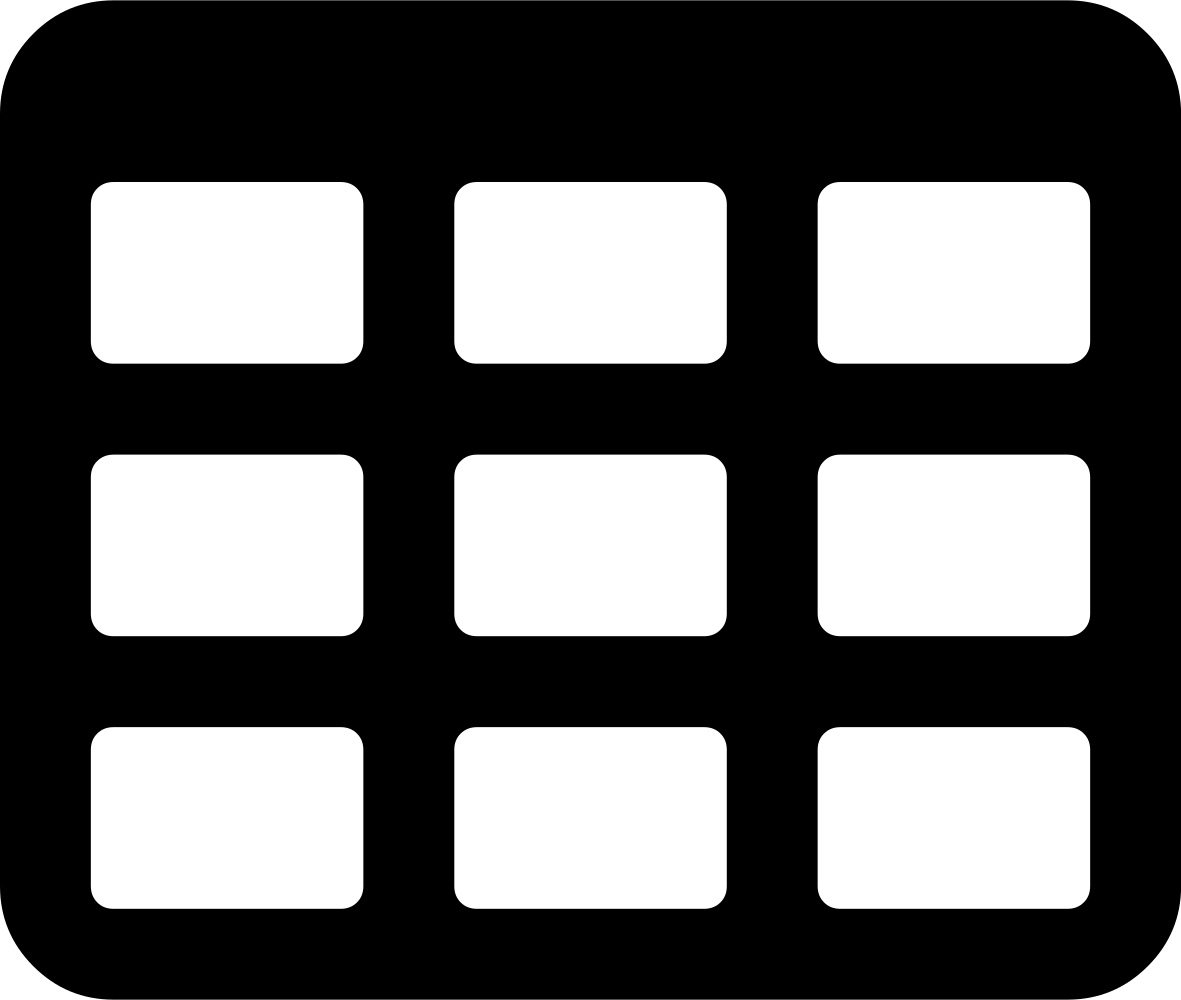
\includegraphics[width=12cm]{figures/view_data.pdf}
\caption[The GUI's data viewing windows.]{The GUI's data viewing windows.
Top left: the Tao root window and the menu shortcut for viewing data.
Top middle: The d2_data_array window, which list the currently defined d2_data_arrays for each universe.
This window also includes links to view and edit (see section \ref{s:gui.data.edit}) existing d1_data_arrays.
Bottom left: The d1_data_array window (in this case for orbit.x), showing all of the datums in the array orbit.x.
Bottom right: The individual datum window (in this case for orbit.x[34]) displaying detailed datum properties and allowing the user to edit some of these properties.
Top right: The bulk edit window (in this case for orbit.x) providing controls to quickly edit a few key properties for multiple datums in a d1_data_array.}
\label{fig:gui.data.view}
\end{figure}

Figure \ref{fig:gui.data.view} shows the various windows that the GUI provides for viewing data and making minor changes to data arrays.
The d2_data_array window (top middle in Figure \ref{fig:gui.data.view}) displays all data arrays for a given universe.
To view any existing d1_data_array, click on its "View" button.
This window also provides the ability to edit any existing data array in detail (see Section \ref{s:gui.data.edit}), as well as functionality for writing existing data to a namelist (see Section \ref{s:gui.namelist}).

The d1_data_array window (bottom left in Figure \ref{fig:gui.data.view}) allows the user to view an existing d1_data_array.
This window displays important properties of each datum in the array, such as element name, meas, model, and design values, and weight, in a scrollable table.
To view a datum in detail, double click on its row in the d1_data_array window.
This will open the individual datum window for that datum, displaying all of its properties and allowing some of them to be editted.

The d1_data_array window also allows the user to edit a few key properties of the datums in the array all at once using the bulk settings window (top right in Figure \ref{fig:gui.data.view}).
This window is accessed by clicking on the "Bulk fill" button in the d1_data_array window.
From here, the meas_value, good_user, and weight settings for the datums in the array can be edited in bulk.
Changes may be applied to every datum in the array, or to only a specific range of datums using the range specifier.
Once the desired settings have been specified, clicking the "Fill and apply" button will edit the d1_data_array as necessary, and changes will be reflected in the d1_data_array window.

%-----------------------------------------------------------------
\section{Creating and Editing Data}
\label{s:gui.data.edit}

\begin{figure}
\centering
\includegraphics[width=12cm]{figures/create_d2.pdf}
\caption[Data creation window.]{Left: the data creation window can be accessed from the root window's menubar. \\
Right: The first pane of the data creation window.}
\label{fig:gui.create.data.d2}
\end{figure}

\tao data structures can be defined via an initialization file or on-the-fly via the GUI. For setting up a data
initialization file, see the \vn{Tao Initialization} chapter in the \tao manual. To initialize data via the GUI,
open the \vn{New D2 Data} window 

The GUI also supports the creation of data arrays on the fly through the create dat window.
This window can be accessed as shown in figure \ref{fig:gui.create.data.d2}.
In the first pane of the data creation window, the user can input the desired settings for the new d2_data_array.
The user can also select and existing d2_data_array to clone.
This will copy the d2 properties of that array, as well as the d1 properties and all of the datums for each d1 array.
Once this information has been input, the user can hit the "Next" button to go to the d1_data_array pane.

\begin{figure}
\centering
\includegraphics[width=12cm]{figures/create_d1.pdf}
\caption[The d1_array pane of the data creation window.]{The d1_array pane of the data creation window. Top left: Here, only one d1_array has been created (called my_d1), its default data type has been set to alpha.a, and the start and end indices have been set to 1 and 12 respectively.  \\
Bottom left: the lattice browser for the ele_names that will be used with my_d1.
Right: Here, the user has defined three d1_arrays: x, y, and z.
The data type for new_data_array.x has been set to velocity.x, and the start and end indices have been set to 1 and 12.
Here, the user is currently editing new_data_array.x[3], where the meas value has been set to 0.2 and the ref value has been set to 0.4.}
\label{fig:gui.create.data.d1}
\end{figure}

The d1_array pane of the data creation window is where most of the data array's properties are set.
This pane is shown in Figure \ref{fig:gui.create.data.d1}.
The d1_array pane of the data creation window displays each d1_array in its own tab.
To add a tab, click on the "+" tab at the top of the window.
Tabs can also be removed by navigating to them and then clicking on their delete button.
An existing tab can also be duplicated by clicking on the duplicate button right under the delete button.
This may be useful if you want to define several d1_arrays with many of the same properties, but want them each to have a different data type, for example.

The next section of the window holds the d1-level settings for the array.
Here, the d1 name, start index, and end index can be set, as well as the default data_source, data_type, merit type, weight, and good user value for the d1_array.

The next section allows the users to set the ele_name, ele_start_name, and ele_ref_name for the d1_array en-masse.
Clicking on these buttons will bring up the lattice browser window (bottom left in Figure \ref{fig:gui.create.data.d1}).
This window is essentially identical to the main lattice window for the GUI (see Section \ref{s:gui.lat}), with a few additions.
Towards the top right of the window, the user can specify which indices to read the element names into.
Clicking "Apply Element Names" will then write the ele names that are currently in the table sequentially into the d1_array's datums.
In the example shown in Figure \ref{fig:gui.create.data.d1}, new_data_array.my_d1[1]|ele_name will be set to "Q00W\#1", new_data_array.my_d1[2]|ele_name will be set to "Q01W", and so on.
If there are more elements in the table than there are datums to write to, the table will be truncated and only the first elements in the table will be used.
If there are less elements in the table than there are datums to write to, the elements in the table will be looped through so that each datum gets an element name.

The bottom portion of the d1_array pane of the data creation window allows the user to set the properties of the individual datums in the array.
Once a start and end index have been specified, the "Datum" drop down menu will be populated with all of the datum indices.
Selecting an index will bring up the datum settings for that datum, as shown in the right of Figure \ref{fig:gui.create.data.d1}.
Note that any settings that have a d1-level default value are automatically filled in.
Once the user edits a property of a datum, that property will no longer be auto-filled from the d1-level default settings, even if those default values are subsequently edited.
If the user wants to explicitly fill a d1 setting to that d1_array's datums, they may do so with the corresponding "Fill to datums" button.

Once all of the data settings have been adjusted as necessary, the user must click the "Create" button to create the d2_array in Tao.  Doing so will close the data creation window.

\begin{figure}
\centering
\includegraphics[width=12cm]{figures/edit_data.pdf}
\caption{Editting an existing d2_data_array.}
\label{fig:gui.edit.data}
\end{figure}

The data creation window can also be accessed from the d2_data window discussed in Section \ref{s:gui.data.view}.
Clicking on the "Edit" button for any d2 array will load that array into the data creation window, just as if the user had cloned that array from the d2 pane of the data creation window.
This is shown in Figure \ref{fig:gui.edit.data}
Note that any changes made in the data creation window will not take effect in Tao until the user clicks the "Create" button.
For example, clicking the delete button for the orbit.x array would not actually delete the array in Tao until the user clicks "Create".



\chapter{The \texttt{report} command}



\newcommand{\CESMD}[1]{\texttt{#1}}

\begin{document}\thispagestyle{empty}
\begin{center}
\includegraphicsembedded[width=0.6\textwidth]{%
iVBORw0KGgoAAAANSUhEUgAAAsoAAABqCAYAAAClFXeHAAAAAXNSR0IArs4c6QAAAIRlWElmTU0AKgAAAAgABQESAAMAAAABAAEAAAEaAAUAAAABAAAASgEbAAUAAAABAAAAUgEoAAMAAAABAAIAAIdpAAQAAAABAAAAWgAAAAAAAACQAAAAAQAAAJAAAAABAAOgAQADAAAAAQABAACgAgAEAAAAAQAAAsqgAwAEAAAAAQAAAGoAAAAAUmzrsgAAAAlwSFlzAAAWJQAAFiUBSVIk8AAAQABJREFUeAHsnQl8VcX1x8+972UDEkBERQFRcUWWJICiteJSLWprrQbrhpAAotb+61Z3jVq12latuywBsWpdWlu1al1xRZCERXBhXxRQRCQBkrzl3v/33JeXvJe8kB2SMPPJzbvLrL87d+Y3Z86cETHOIGAQMAgYBAwCBgGDgEHAIGAQMAgYBAwCBgGDgEHAIGAQMAgYBAwCBgGDgEHAIGAQMAgYBAwCBgGDgEHAIGAQMAgYBAwCBgGDgEHAIGAQMAgYBAwCBgGDgEHAIGAQMAgYBAwCBgGDgEHAIGAQMAgYBAwCBgGDgEHAIGAQMAgYBAwCBgGDgEHAIGAQMAgYBFoBAlYryEObzsLll1+e1rlz56Mdx9nPtu3NPp/v05tuumlFmy6UybxBwCBgEDAIGAQMAgYBg4AYotyESpCfn++3LOsaohjiuu46ztP5LeV6Es9mNyHq1hW0z+hU6eobKuIulbkFa1tX5kxuDAIGAYOAQcAgYBAwCLQMAnbLRLvLxDocYnwmx2RK/Fd+H+C3nONX1113Xfd2g8Ju1oliubeL7Z4i2eM7tJtymYIYBAwCBgGDgEHAIGAQ2A4C/u08M4/qRuA0vBQedthhr40cOTKs3pEk9+Hn5JSUlH343XDbbbddi1rG0Zy3Fay/DQaDN91xxx1ryLPIwFEHiSsXMvcwTFyruziB+ZSykMPxnpt/BgGDgEHAIGAQMAgYBNopAm2FvLVW+H1kzBclyZpJSHEYXeXK/CJlnoVKxrfcqLpZ+bRVnmxJT08v9nKmKhe2/QtI8olcJ3EcLJZ1ufRffKl8JptaZe5NpgwCBgGDgEHAIGAQMAg0EwKGKDcBSL/f/1QoFHoGKfKJHG/dcMMN+0CSf0mUSiJXa9QQ5Q/4+Wjjxo1tQh+8W7du7jXXXBO89tprRbq6R0OSLyL/XbQsOBuinCP+tJc4f5bD1ZvGGQQMAgYBg4BBwCBgEGiPCLQJ8tZagR8/fnxSz549L0OK/EfyuJkjFenxR5Dlq7F88UVrzXe98pWZt69Yzt1w47O9JZ+us1LE6krYzhxljAB6y9ypG+oVl/FkEDAIGAQMAgYBg4BBoA0iYIhyM7w0pMl7EM3QcDi87vbbby/ivG1LWvteliIZW8+hHFMhx/r3Ksc1kOOrKdk5SJWT+H1Diqac3AzwmSgMAgYBg4BBwCBgEDAItEoEVMfWuEYgADnu0L17d+fzzz93Z8yYsZXzZXvuuec6zts2SZZ8W3ptzMLKxeNi2Rlw/vXiOvdJ0b7vyF4/fgVJ/glw7SW2v6/0GLRE1s1d2Aj4TBCDgEHAIGAQMAgYBAwCrR6BtrLArFUB+fjjjyehe3x7v3799tOM3X333emHH374iUiUh7SqjDYmMwPX9xC/eyWL+PaBLJdxvCKWf74MWJaGqsXnEOXJSJc3iRNi5aIUyMALD2tMMiaMQcAgYBAwCBgEDAIGgdaOgCHKjXhD69evPwtd5NHoIqdo8OLi4i4Q5zPYle+YRkTXeoL0y0mWpOBpqFX8GjULh98PxbaeRVf5KElKysQknC2/6PUYuhiv88yBRKeIz/cn6X+u6i4bZxAwCBgEDAIGAYOAQaBdIWCIcgNfJyoXhxAkn+Omm2++eVEDg7du78npAyDIN5BJP0SYHfjcp8Xxz8N+stqBPkMyV3WTfOwn2+5NXC+rKMwJkpR6oUeiK26YH4OAQaANIpCT45Mho/eSg3PTW2/uGaxnn99DhuXt1nrzaHJmEDAItCcEjHm4BrxNSLKaSbsJ6fECfpGstiM3LCdNyt2bIcW9KNVW1CteEivpWfElpUko7EKcz0Qd4x0Znv8/mZG/XLLG3IZkeQp+0zj+T7JXz5FCJNDGNRyBARd0FLdTsiSHHSnbVCqLng9sN5Lh+X5ZtzpNvpqyhXfQxnXit1vSyEMlRTOn/FAPn8ZLYxDIHo8lm+AhstTKRLWqv3QKv0k0/25MVC0W5mjIe5l7mLirB4qTNIi2ajFp3d9i6ZmIDQIGAYNABQKGKDegKqBucTbe94Moj4U0t6+d6QLpl0COT4EQhykjAwH7ISmcuC2yZbVyMWtfpM1ny+bVc7lYK0VT/y5ZuT/lfBzH3oS7UjLHfGVMxoFGXU4ldys7ZknIPhSpfW8WTSIdC6SwaNKR5E4l4Pod+K9Gcr9Y5vT6HGl9fF0rXtNHOsgIGTCqgDe1tdbkssf3QJd8J1m2cYNS0qlYlj6oW7o33mWP7i8B9xKknH+QrwpKGh9RLSH7QcKT3dRantZ9W/Ht0O0HmXlfqeh7XdxtL5FtvD5/wwcwGsYJhvjOgtIjvVReayJ2deV+4Kh9xJd8BHXkKL59tZk+FKJs8y1rnWodRHnImF4SsoZikFJ3Bj2KfB1JHqnTrg7KDVGu6x2b5wYBg0CTETBEuZ4QQoyPhCCfSxs9iS2rv6pnsLbhLWv0kXSOqnKhVlC+p6N+UOZOrmYH2uv3jxa/T/WRUcvAuZJP53okZ/05jqUDgzTn/6kGsVO/xkUQyBp9jCy3zmLgkc2NvmC2J0cFOsCvp64LuXS+EUeWS/aaBRLO+wC5/fueVFWlzyKjPdw7Jj/Fee1E2Q3diz/dUTGxs3iDrpdi4uf1uVtbHK61UtK3PkkU8+sTTa1+HPsqZjJGSUdnDX7urNVfYx+kuGoGcTBHB45kDq3o8QMTblRzuvEOhJL35PeFpWzzgzyfKV9ndBY7eI/3GVkW5NvVt1kzrloxC6H3b3NIUL7dViqZuaWsEdgojvud+JxlpPmlfDpVcWi803UIyemHsnXQCUQC+XSwcCP7UvF8XqQuxdc87Ew3nB1BSywWCdvHS9jV9iWLt7JfTJbIn7Vz8xiTGXNqEDAItG8EDFGux/u97rrruuFNd6ibX15e/mrsltX1CN66vfTL6USHBLnVzUTcAJ3mM5KyJbE0yYJIOMEqvfa5BWslK08J9tOE7UpHfm6FCsYbrbvQOyN3SBuz0q8gZSVm6IJDTCwWTKr03nEXIj2GEEEHbHd33sVBvIfD+d2fO8Pxd5qUy2IkzUu5n47/0/idV49S5OAnQoA8z/A2pW6xrvq1EqUaLkG4Gn5iw+HfdjElaH+At8YT5cwx3cnvTyBzmtpVqP3cg9oP5laa0dnWp2D8jUgY2+B2H7A+BciGV6RZW0JvQJJfo5Dr2LM+JGF7TcRjcalI+r88kC2nqzgW0k8k/2LtzfdRFVflaSyunMe5Ck+uu404isWxN1Bn1kOeC8VnPSdzpujMTsOcSryXpx9N3m8lT3uQpd78ojpVmaGGxdcSvlWtaPOaHN7DWPKl9ukPoPwJBnsJK2pL5MjEaRAwCOziCBiiXI8KkJKSoioXu2HlYuKSJUu+r0eQtuMlJeNaOqRhFZ3lYvHZ98nM5+nw6+lCgXfQY34YkqwbkhzIcaEMG7VIZk6HfBjnIaAbuHTecgd8ZBTX3T1eYrEY0pG/QChnQ7Z+QMJXJn6m3gOqBuB24RpVF/kF5+dCFA4iHIfLe0H8bAl+6qWbHEOSvVSxia369dYG4tDdFcv59Viol0/XDRH9xfgk/hhnOYsgae/hV9Vyok7tniTjvyNZ2Y+bg/GjeeeUw1UJravS78Y7y/4/4tjTi8Cyu0rJmtM4TzyIa2wqc6bMrgyq0np/CuYQ5WLKdRn4VD6KOZkoEnpYUkqX1PhOIt/NPz2/2eOTILeviS+wnOvfcvSIiSNy6jrvgdMq3scq3vdG0tvGQZts9UCSPABPwznQH/ak3XuBs87cHImU9XgI83PSt+R+ef752HfC4+245593JPvC1SJ8r25oLZL6gxh0/Z4QDMpaiZtBrRoU/pJB1v1g8B3560PO7uFgsGGcQcAgYBDY8QgYolwH5qhc6AYbp6Ny8QJbVc9/viEdUx1x7/THg3NH0C1dQD6U8MBJnKtk9qSVIpPrn7UFT26TrLFP0MEfRxzoOKLnXO6bL31H/E2WvlZe/4jasc/OW5G6W2MoIbrI4CxKVp0xYid96emB1yz6KvRdF8oXnWdJUugf2LG+nzCQGaR/ldxNp/U1rlrcoNFdYp5sxu/jvKOnecebISEBpvIdKWfxoC9Gl7aDVSalMppw8UTZlbnic/8kIch1rAunWBBBP/kjXwH01O2xZEkHA+o6kF6nyGkj/vfLT2bh1jHEB+HGRaTKt3PWvETZi7zi34InVY3lC8nM+ysk7TISjX2q55sY2MyQOfsvrFO9qHBiEP/fyNBLH5dQaRbnZ2oE8c6+UGxfQMKBUgmGg7IbahzlXS0p3ZRC+un47cXQ5He8u19x7pmi5DcdTIbwu58s69RLhuVcV4Ow87AW50rhtpWS3XW1FE4LyoALisSfzO6aWrdai8unTo6fJ+l7z43MHuTPZJZKBy0MNLSRMs4gYBAwCOxYBAxR3g7eFSoX5+NlKTaSX7/xxhtZpdNO3NBR3eiEf08nycYiaFO4zp8lY8XbdEY12EEdJXYlo+cSKV5zC/5UmgZBQwUjvUcR52/VEbb9P87KHUknfy6YoNqC83iydaYUFizjqnasIwOyb0Vyvpd+GcdCk54j8AnbC+LFH/3nY/fESOxbebd3iZ38oBSxOLMulzUGCXM1PuKqtHvL9/Lp9mYa8lfI4V8vliSXTWkg1eIqwW28RDlp9TjiOIS8xGZmPySiB0jhE4pdy7lAykZJiR8TVCQ2Txzf4jpJcmzOZj+8EQsxOlDRtxFbFpG5U1bFeo051xmdH0nnGzl69WdSai3l+hrwiLbXGk93osuVsk5IoVlfoHrP9XJIoAsrZgZ0YJCV1/oGs5FBRkVpIM5O7kKqwSBuRAcL9Sqp8WQQMAgYBJoDARiScbUhkJqaehrP+nI8C0leU5u/Nnk/6L+KrnUYefcx9f8NUsEbZMaMUKPKonqjTvgTCOFfPdItMpCOeyTTw7v2dKlOv1tyKoSmD7iiMuHjR86ToilKfOpPbBZhGi0UPJ0gS6pzLY0woQtDlCNpfC5zp91di+Q6YdDG3YTQLJz8LTrsf6dkU6gH6L5WSIMbE6HqJouFvnacQ3LtmxR3p+UuwgmiXoW2LIOXBjq3wYPPigTA9CMsfRRNuZFXie5zDafS5TwZPGZCjSf1vuEE8MrgqBU72/qS3FVrm+IGUK048yZrBgGDQFtHwBDlWt7gbbfdlo2ViwtRt3ht0aJFH9XirW3eHpQHeWP3PZ3GtSFvln0KREqnihvv5k37kXheQHo5J0LmWIxju6djXi7BQpzGJ9OmQobDv6ocjGjGvb592xuNKoNK/6zwCAhT/Qi234dOK0sA7ZQLGpVeYwPNRzfdZ79MNnVhqI4M4qWo9Yl30NifEaw/Iau3T3p9aIvXKV+JYoxEt4bbikm/hKLmGj6b+0ZRwdnxwvVoAizKcxiYHnFeRvROw35tnWWoRkIbFkOL+7bcTaSRaODS4kmbBAwCBgGDQPWOyCACAnfeeWc3CLJaDPiWBXxPtSu9ZN15y+eOhoSopByryc5tUtQTnctmcEWTFxDjn5hl/sFjha51iYTDQ0mm4WSpGbKz06Ow2SBBF2bFuvSULbGXDTr3h7B8IE9GCFMdUkrH6YFfR/b7fkWD0mgOz6HwBsr9Ja+d957fwHefb4sd/iX182Av/zXz05nZi9tr3m7GO0lpEGW3hDJUjzSIPvHOI5WWdWNCsmxZv5ZQ6hnVM1vPax0gt26JcthC6l19fFjPAWM9QTDeDAIGAYNAbQgYolwNGRbvJZeVlQ3n9pEs4Cvgen01L233Uq0vhOxx9DknUgh997MlNTixQTqXdZU+KaTr1qfhTXUfD4drnCdDxkQsF9QVtr09t3TXQldt81a5H6stlKt6UvfZrKeKJWz9GWktxKaOwYdloyvuLsMqAiRjBzvLWslg6WNSDUrOohpsc7u5yVyleslq4UP1cT+h/kBY41wacf+CRWyq2tFyrjZ4w4GGlac5c+ja90Q+2xqR7o51iOpqKjU81XKj9RNlS+2K1zEwrKVw5rZBwCBgEGgqAoYoxyAIKVY8DkOKPJrftxYuXPhOzOM2fkrZumw9HonUWRSkCwRkvdhIk1P2b7jO5faQmD19I49fgOjM5pfNE9w8yPmpoiR9V3OOQPZ0pWSFUyGYz3d09LJRv3ZYJdKLObZP2Fx3Hl7ubVQaTQ3Uefl3RPEcA7LZ8ny/6qLA7cVOmexf4CGK0R+JYyZHvMTTlW5SloHO9i7mCifWLs22a2P2dWGEScDWLlG2VKJMLTDOIGAQMAjsBASqOvGdkHgrTFL1/FTlQhvmye1K5SJzTS82QDiXcqkpKPQs3clSnjaz2TdwIHKZWwC5sZ7g7BsOTM+xWURG6cH6aJdyno3imCniiImzu2XQ6D5NwEF1Z1/m8FYG1hpPUcGLUlQwrdbnLflAF4UWFrxLPXirQbMVA8ZigcWrn2ot4zPGGCupp3dzL95ahyV7MAAbI8OHq9TZOG/Q1I6b8rBRTzaV3CBgENh5CLTj1rVhoFZIk49H3eI4Qj7crlQu+l3SCcJxJuRCpXD6zj8SN/y8fPZoogVLDQOuNt926X8gOP/lMYvQrENY5Hcli7A61Oa9Xd53LTXzpVPbFU6FYlY/Nnq4TbJHo2LQCDevTzGytXcbEbL1B/GFj6GeqlqQugKI8iopmvoO9XZV5Fblfwt/vaW4j1ptMQ4wWpVQOHt8Z771HpI9qrd36LqIZv/2a7V6YcmwvN1IrzcqX7347WwqiEHAIGAQaAoCRiJThV5vTn+PpYuX+J1RdbuNn+m2tUtLsyGreZA0NjFwV3L+uJSVqsmllpvOLHzmexmcNxV92oEcR7CBwig2pfiQNCe1cUTrn33LXQHE34O71q2Ii0iVsURhp0t27qNIXt+IPqrfbz52ZdldzbZnM+SJIeH1C91qffW/mC3QA2zMwU58lqyAJM+TORN1oAEHtO7j3uT4vFv7getvuKd1quXqcXyiO/dqeL5PSnSSpoYLM4NTu1pGDe8tcCMzb1/alWy+9QPFCe3N+0pHzTyVV8O7YcDohn7AXOQa6uxX4i//RFTfvjnd8NGpssXH1vCYvCwnD1a4K1uLo7IT3Eg7tJQFoHOkaNonzZmkicsgYBDYNRAwRLnqPV/H6Q/l5eVT7rrrrnidyCo/be9saboSjwlk/DD6rDI6s2eZtX9XFu2ARV66PXBmHgTH3Z/0WdBn3yoDct+XBQVftT0gG5Fjn/s2i+90R7aeHPGzN678knv7sxlFPyyDPCdqVq2+znVWYq1kkiStiRDJ+oZrzf78ZZAcS61d6NYZ/4HYLCK7EQI8t2CKZOXezzUzI5VOdd77sSvkIVI0+YvKu+35ZPOacxhw1iyh6y7EvrTiteOdDsSXdGKXSTmNWSPsp7v7QowZHLI1t5dVix0b2X7aU9V32PxGlkswZQ7twjQ2XHm/WTKskutiH4Mmb8ZsEOmzK2Q0Zj47bffELiLN18QOTpfC6aujT82vQcAgYBCoC4H4zrsu3+30+c0333weRTspGAzeCUnGtFU7cQMu6EhnNZLSnA5B1kJ9iGm4Z7CZrAvudoxzw/8iD0hN1a4uptL88kDzT8PumKI0OJVPp64hDPrEVqIFk/rtDeDZDSzw+yvSthHSLye5XmmoTeUFT65o9AYx9UpkB3rqgzTQstRCyoGkqnVzDvrNSraqnCX3VV1Ung3EvK4u/kvAHiv9tJ8Ty70NMpqgPPZM6ejseGnpCBboLkv/C+T9VogpbYwOCO2HeR2juHcppPm3nOfxblmU6ei3oLrn/TnG8Ow+GZiH6cgmugG5mBH03UL7chUxHcWBepey5JjDFSTb+sy9RsR/O4MrvjvjDAIGAYNA/RDY5Ykyush9sHJxL7rJ9yxevLiwfrAl9oXt5VbUYedjj9Z3GJ3U7+is2NHMXc75VOnQu0pSl7gY279r+SplNdv3WPFUNyIJ+/7I1QpvFlYwTeeG6UB3EedP+ycd9OuUFqlWQteN93MGJOM+Sel0D7rLEInGWjBIGH/Tb7Z0K5Hh6wuvuRAc9Pt5neKjTlHNHFjYuZdn1VVNuuDvcMkc01jTaE3HZkfFkJWn5e+TILlPUTN4xtvBL8HDum9Vw7nuAFU+vt36Vy7GceztEVPXnQ4hxi77lNdFZ5MKp87yzpOp2678GX9rqwJLFhsSQaqb4AZO2IedEm+jDpzN0Z2DyKJHgngtZiRcweqPcx1k+dAEPswtg4BBwCBQA4GW7gJrJNiablQs4NPG/hN0k59oV1YuBixLQ4/1ZsjpfnQMOkX/uvg7vNIiVi7qeqnzJy3Gy80cSnRs+rIJSFAH1xWsXTyf/fBGCbi3UJa3OWpbvq+S5IPhibmoxUxHd/laOWLsnu2i/HUWggGdz+1FnUA/GdvbliyUvsVf1wimAy7XejVChGKeunIcW4OfzB1lSO3TZY25ASJK3ajhVEo7SYrT1RTjjnWD8hjYiKoVqZRYeTLGEMN/kLlTa87IzWQLdtsPiWawHOssyWaQc2zsrQacdxV/4Bri/AWvfiME/XHauVzau9O5N4p7jxDX5gTxdaCmnEqGR4vOuBlnEDAIGATqQGCXJspIkS8CnyHbtm27FNK8rQ6s6nyMZNqt09OO8pCUpHrJJ0WSsxaI49wvsx5s+gIaN9w4QlLU+wXy8u8In8FigSV3i0657wpuISoY5bqYEdvC2+Nzri6A0sWP1nUScl5CupwjqgO6s12i2f7mytPA5T0qZj0op/se56+wSUriAYXrv7oGfJbsA2YHSt8R9VNbaa5874h4dIFcVt6T1BlVK6hmvcH9DnKYLymd/y5LHyxvfHYaOXthuzmkuUdlupblSMSGeuWtuJPCiUpav+SIzau2JWPi/NXvgnCuzkKcT314haE3W8W710pxp6el8/JXJVD8LIOn69H9P5rnH0YmKmIi1u9M3PPF7x8Zc9ecGgQMAgaBhAjsskT59ttvV7u+V0OWr7znnntqSrASwtVGbmafr9sX55NbJQ9rIV73y7xpS3Zu7rHWUFRyDh3aD+RNyd9g2c1/7c7N0w5MfRFStblTzmOTl8siqdY63tAHEGYZIq79jCxN/59kX3jADszpjk3Kj/WP6IDOtZZJp15KphI7Zxt1WVZXG2xYEKVfSuce6KC2A9d3RIpkjT6GxYsPo33yMYTuXEqFiglONVM87RTrbVQOjpO5fabJzPt0tmjHusjgTU09xvQf9VA7szyzhvFSXts6shGZVyCARv6OzvF5qHnMo3370RswqA1vXaisxHz+E4skGPw5AwrUU/SzinWuDtAGy0/O7Rp715wbBAwCBoHqCMQ0dNUftd9r1CyscDj8R34/5PhPuyupm6zT/J04dCr7PQjaP1pHGZEUWvavKvKSwVTpeZI9RqfcdxGHPuicqQ9JqLxXpPPW8UKtTnt2H4uiThA7dakMzn2I6+q9fa2B28SDfjlaR8dBWGiH3M/EF35xu6pBCw4ohZqdi0pRfPFcGQRpOozNTao9iPfW6q6y8l5AzeZppMYvcrwl2XnLJKNHmdhJ7/OdXEJ+9+ZAVUmLxat3nH9J0DkSvd8TZdbUzxu0mUtLF96qx2yabZHnapvHON5Cu4bmzmHwX8SCz99BiFWdq/aZPF34WjR1KAN09RfjYM6unCHbUn8Wc9OcGgQMAgaBGgi0rY6lRvYbd+OWW265BILcm9B/QuWiWgPauDhbTSjVZ7RsXaiinccyJC5Xtpq8aUaKJn9Ap/VERZ4OQGp6xy63KcCCp76WvluGYQLtYnBYBwkKVeBR80fN0Iapog5WBLLyVmJO7mQZnu+v6bEN3unUuQvv//cMGsi8+7l0Wvnu9kvBrIQVXob/knh/Hk/6iQz9et/4+639yj2Vr/TXlH0Ex9F8F728HDtonkStWyhJdtxzIMcW+r9nygIWyO1s56nGWCvIhpp705cXIo+f1pmtgPWj5zfWY2OHfpa39XZsTNs/d9hIyhtwxHnbnfzvFnfHXBgEDAIGgWoI7HJEGWKchS7xrzkmgsVyDq+XrYZL27zMHo901ro60snSKVlOPhIXiFgzuoZavUicNHl01fqGxfTyUJjgJZDlpMRe2+ldJRtzCx4Ty69Tz1oX13IEai+tVlMd3FnPSfHXN3q7j9XuuXmftEQrodtPB9yTIC8a+3okhDPqZe7O35Wpe/fOBKQnR4Lh7DYlVQ7LKciL0ZO1mGVxVc/2L2CRQJXCObrVmVQc7JvA1/tHjlfJ80PSufdPt1PpLG/hXLKrKiTValMNnYjtRBP7qIHNts+HrWlnVWwMnNPmWLvLsJy0avfNpUHAIGAQqESgfUimKouz/ZPrrruuGz7GcXyFRPl/kOay7YdoQ08zx3QXJ/hXOq4Mj0S47r8lvc+LrbIEnffdJD+uuRGS/AQECYkO22vbzkxIzvscKqHadVzhxNUyfPSVstl+hXendXMYB6auPD3uRDioysrlLA7sIgMm3CkLHvsukadWf6/kICwOhO6EHGpWv0BqzqK1ejjVyc0a+x9IDzMnnnpRNJCqqQyWfmvekUXyQ/Rmq/6dX/BuXP6yxq7m3R7CvV9yRPRyVLJs+3/LznYfcO+5OP8782Kip/Lwp+1mQfWtO+zTXXxOL0zBHY3UGem5t/lOTLAd9rlvQ8XnHojxw5XSes2F5faXUHoPzpbHZMqcGgQMAgaBSgR2GaIMKU5m4d5ZFSoXd4OASvDah1PrEbZ9MbJxNbnGZKa7GEnlDdvV99yZJZ+RH5L+F78ndmA6eVVdzGwJu+Mke+1yKdTFWruYmzFNB2yvQXwLMXml1gSUUOi71IVuiSanIcvueeILrkPS+CCzBtvw17acGx4GccEEnrdb5GpJS+nKzmm711kIGzve4UAnwjKwsn9G+Ngg4yQp/E9ubOKIexDrqdWe6w6DmbmTIPwHMYDoV5lPF1UMkSdlyOjF8um0eZX3m+VE7Sg3M1QqoQ107Ev2+kP8Tyb6E1Ed8vHOviYtVTPSRcY71hVODLGV9ZwERe3FVtdmQd+OfRsmNYNAm0JglyHKLN4b6PP5Tkbl4rW0tLTCq6++utlFGTttw5Fu9k+pdefRCeniqG3sVPU7KWpmlYvmrtafPbpJBo57UOxwJh0oZpyYhpfgLKZop7Dr3NbmTq5NxBeRDj+MWbi3xbFZtGb9AsI0gLzbCfIPqXR+g5SukGdvczQz24lNMVHysc8bc+7eUTEGCFPGvSSo6hT1iEd5lu3TwWACssXshA+p8vDRn0lk8FGPCFuZl7m9sXKyqg/Y3EzO9qrKnZUMoXuMAeYI0W+nNTodsHezB0sASxauexpZHMA73UBZkIa7M6jTC/jen+C+kugd71wfai01mn1IcqjDjs+MSdEgYBBoKwjsEkQZabJ2OOdwbITMvgJJblYi1qFDh1AgENgICUd/cge7ARfsR0d0CR3TfhBOEncflcJJ/2uxXDTWjnKiDG1NXSUZpQ/SeR1IGfaA6l0gvtT5qF/Qse5iKhix+BRO+5LLm5GwYldYB0DeUZMYWtZAno+Qo3NnNX5nttiEazl3apCLWjzW83bmmMPwOZC66pJ/H+99ONdaeevpvDGBSkJ1IW5SZSBPjcO6TH7wvcw9pJdt0VHvgxf8U/xJmZTvfGCp0J/VMltHSFLgJk6uaL6SNdKOcvUMDMz9ifgtpMcsUBRvcPcFXlCtct+WYMpHHrnPHo+KA/aWI+o2FTE0dhDWYN1m6loowOLR+Jy7OgjVgZdxBgGDgEEgMQLtnihDknVTC6SVcijHX7F4sYp7nDafQ0L9Y1lZ2QvJyclbmi/WesTU97IU8W09n47nJ3RASfx+iD6gLghqG043Ssgc8w461U/RuV5GpgfTj45GBWNFu1DBGDKmF5LSVPlR1shKT72iYe9l7pS32aFvIXF8Bj63EVhnDGIdJq6sIVIa1mn6T2IftOpzS1S3VXVwiyEu11O2EHU3Qlasii2Vo9fRglS/r9eWOwSSnYuXKqJj+Q6VlPAhDLTWttnB1oInv5PBox4Vxw9ZRi2psnzeAOFSBlALMflYEIVmp/4OGb2XOL4xmK47g2wOIS9beRuP8D7/TZNU6NkzjmbQCWHzuupVRW/vsF/HQofFw7AqSVstd4S3s4i2yqs5MwgYBHZNBNo7UdZW+SCOM9BPfic9Pf0jfqu1lE1/8VdccYWuVJ/b9JgaGEPnbSfS7qtOqy6I2wj3+KN8OuVbkWkNjKgO72pxNIpa81i9qEpQt7wdMno608qqYnAC5IeFTOGPZNjlT+2UzRSqctb0M0eOR3d8qOxm3ScrZWmjIpw1+VvJz/+bvLQKPWT7Id5ztW/WzWIm4XDinsURfUuNSmqHBBqWt5uUuyeTloqp52Eu8OFGp5uduwJSpjqwPSvj0MVvjlzPYOtjBlttT3c7WpA50+ey8QiDI9QtIvaUo0+S+Eaug0gvlDnTZ0dv7pRftYEetq4h7VOog50gx5sYuP2fpCb9Tz6ubZFp9SrazLMVdQGhPUJsFlxdq+LfXFcw89wgYBDYdRGo1um2LyCQHHenRKMgx6Us4nuqgtA2ayFJoxPqHOegdnEEESthfo3jHe6XNWtC1SMbOIoFP3Iht5GeeRK1hyQt/DGnsd1A9VCt83rb1s8lLf0ZynNwhPQ4V0rgxyJ6NAYfbbA8UZRd2ZNTbOU6z/G7jKNx7yaf6fgBF/xdfMmDkciNhZBEU9DfjhxdsK3sa7WLN2NzG1DdZG8xF9+Ke2vsowafO9QP23qRcL/lqBBVKjbYzHXC+u2v4mi7LmPla1K8/yQKcBWHvmd1Ws59GS9dR504f6fp80c2CtKZgeN4j9qPwHjdUdK35LVatyDH0051djJqPqqtE/P9WGyrHUhav1PzZRI3CBgEWjUC6Ge1TwdRVSsXx1K6IyHJE7lGctC8TtMgxlshyWdBlpUIbSHN3/F7Ps9Smze1mNiGXZ4mfv9pNPg/4y4SJutVrFz8Az3VllH9UE3SqGtOHeVonLrlbCmEx5X/kBIDDAvCbF8tg8Z0jnpps78u5vpsew+PyDalEAue3MZCqAcgyeU1olE9yw2L2sK3zNyE+wsv/5Z8Lwdsea9GWRpyY+7U76kzqKVItXpPdbXcWxoSVav0q9sxW/77KKNauogVvSZxfYIkJd3U9Hw3YiB6cC5brKu9dq99jQhbLPdZdsB7ZceR5PjRYj1woO6Ftb2Ocd5GP6vks0d+jLlpTg0CBgGDQBwCbaFzjctwfS+CweCeEOSL8f/KokWL1AZpS7jDSAPCKtdBlh8sLS39E9f/5vqnXB/cEgl6cQY2s6rcGs95F4jlt5xP4bzxEssWy2gDIl405Qfx+SZDClSFAIdtZcv3c06qSLp3v4390zVHrnuYlC5p6sp6xGDJ64BjeU1IIDupXWPEZK0Uo+y8a8n77p6db8f6QzOQKoZw/nco7RtxJY7sajda+uVUI0ZxvtrGReHEzeJ3ziKzOltV5VxMB7pyNjalWfC3g11HR9cTqPpMBF/9Qn1hvde6nRVOi8+gu4XhB2oXjRgsxEdkrgwCBoF2jEC7VL1AmmtDWFkkhDXPjh0ffN7bcrX53yJk+KdIkpeTHmoCEXfTTTcVYobuGNLvzZ35PLub3xM5VAq0PVed6EQJYgqBTiaelV7gzDymXd0JsK+DPSsXjjuRtVDvyLxpOqfYtt2nk+ZhR/afFOIQ6PGe9F9TsS38TpvdVMN7G/paeV+u7xlOir1bjf/HO2Zhn2UdCkmKOs7cUhZNhaI3Wu2v44wk78levf3WfqlZ8lk4cblk535OXOxsV7FJh0ZssWostdMozibrZZt2n05bL5njTmVTnhl8+7FF2RdB83kydNxsmT1pceyD+p830OpFTo5Pllv9wLprVRoYep49fWPV9fbOtFmLLUNjZTUNtHqRk2PLMncfr+5VZW+GOKFPqi7NmUHAIGAQqIlAuyTKFPOnqECMhMge39ym4KpB+B3XPSHFJBeRSkCS0znXFf3eQiLMxj2TkpLyjvrRsDzXn0qHfefKcz2JPo/e59pOTU3d4HlSKxf2tuFIkCEc3HHd19HFfFbmP9F+pg7nFjwI8RlGX5pDp5YqScFnKelxXvnb6j/LtxeLFQ+UnJxlTZKiloV9kmJ1j+MZuiBOfEoUY9lH60MqK3ckmerlEVjVTV47yfs+miGjSJXtD9ADX0BcmZXxqVTZ8ql+b+OIsve1Vsa280/mTnpPBo8p4F3nxuwsxxbw1s8lHL6UjWeuYrDU8oPlzxmMpNg0YrHVrSlgNZCoN/ZNfJVKW2JdGzPQUKw+lfnTGznAaGxGTDiDgEGgrSHQ7ojyc889l/z555//HbJ6z8033zy/JV8IZuFe3rp16zW33nrrn+688857ILd7cIyFFG/AVJx23MJ9iEyzODanLj4cySSLoTyWvB7C/DQkWUlS+3KW3Eo/TFndw9m+dzjmsH6DOSwlzLG9c9sps6cKYD0ii7sdRaa/aXTGO6BjGbb7Vwv/niSlzal2r/GXrmXXVHZRqV/PxscZqbCqKtTVk+iVhP/alMhqhJ0z+U3JHP1r4h5EUvGsLWvM8ejOvlMjzPZuBEst8Sd3qlHdXGwaux12njrHnKl5kpWr6kh7V2Y/ImEeL25gFQOxvzV4IMYYP/K+Yz4t140fzVcmVtsJgoFBo7swq7W9AbslSXaKhJx4EXLs+gcv+nxbchZZdZcjXrReW84q7/vdHgychkY2BqQdcd032Vb7X5XPzYlBwCBgEKgFgfhGqxZPbeU2JNmHPvIT5HdF165d72+JfKtaRzTeq666ahtSayUAR6ITXRgKhV6CJKsu4YPXX399RAoc9dzU38xcjPX7/gAP2IcOHMP58g9JLvsP0cb0cE1NpJWEn1PwFZ23SgM3MzUK93GnoYt5SCvJXeOyYUlv8QXukuxzdm9cBNQ7x3ckYMSEt1YT1xyZ9WBJ4+JMEEo3AKnuLMjN1u8r6331x3VeZ+X+Cj99yTtlCK2UrwqaL7+VidtK0lgIGuM8qbL1d6Stdak9xQTiNJwO2XZrLiS12PnSH6qm5xofNOGV1YxS03BoKGlsqZZOKmbkLpelnUY2WC/bcjMoazXyb+9WLf6qy+79ENVXI6l6adsMZKvaxqoAnGWP78D3ewQkeTpX+8U9i61vurNf9uoTZVnGz+L8JLyoNiBK6KfipqernnwHi/n0Bpl117DHyL8ksrHP9kKaZwYBg4BBQBrf+bVC8L744ouzkCSPgLxO+N3vflfTOkAT8/z444933nPPPX963333ddGoVN0CqfWnnJ4MUR7B9ckcF0Gmm3c6Tzt6S1g0aP2aLYvpqOQDDPw/IbOeKtZ87FDX3HaUa8t8ISoYkUVaWl70tJ176HBrkpfawre2+0omLPsCkbS/ssnKYQ0mNANWDYKfYHO4cly0hQHE0xIK/puiVt5shmJDuqo5y9sdLmqerNrDOi4PH6sm8lAXULULFfZaOpBtfmc7qru9vkbELjbG3XBujft13mADn5quBwSrdhJZ0z93lDwyQOBfjccD85T0Nsx1Xf0tbcBvCRTfvlmI/G3reknNOEWGQzjr61zsH8etn1Ae6a2vSBzDjHz9HkspTbzOmFrgyVwzmrqNWT4tM8cR52VAkNGnD1/E9zuNcHtxBDliHOpVA0ftgy31vbA3fjr15Eoy0DvGQ6JTsHS7im7okwjX2BCqrpac/hukySMpl34nG6knk2VOybRYb+bcIGAQMAjUhoA24O3C3X777QfTDt5CYW6EvC5q7kJBknuzcC8XInwXOsP7VYs/0Llz59XcWwtJRgTazC5Udjgx3kjnoKoya+lMnmGac14zp9L6ovPb15KplRUZwzZuaFSkE259Wa1XjiIqGJTBmippGb+WQRcdWCep6X9xV3S2dXvgaaQRnXLfRqf/T3Gsx5rVjm5m7pmkUU26yB2XxZXJvoGc1SR73KzV6cAm2bmY50cSMtLWWN7mOA2Lp9YEYh6oyoi3HXHMvcipDrLukAGjkcYrgauHSy7TxaSJXH8wP7xBEupBKw8gouh7i4/T514ef6MeV2oyzpekgyO1zR3vXG/jmbulxDqbPCrZTFyKaKh+mLe0XPCp5s+SQVEvCX4dKgQ64VJtUKIqHO5jkNBbJOub0yVrzakSSOXdO1O4fw3xLEHsfBEpaTsZ69LF55+EStGNPLuJuBeLFXg51gMDAHZwjBsYUC5MSIblYRmcd1StA2jd3CZj61nk6YkKafIG1NUmyUbnzyLPVyP6cSmaC4OAQcAgUIlAu9BRhpx2QTf4BojyIojsI5Wla4YTCHISEuoBkOQxLKzbj98Hvv32289io4Y4p2/btu14/P3A/fdinzX5XKVDxfZtxKPSk60cr0g4+I8mx9vYCFrCjnJteZk9eYUMzr0VE04T8dKRjvRKGbSqkOVrH9cWpFXeV9vQrmzyyqB2lS1rKFLB6WIH/ycl/jclK28xizI3oo+NuaoQtnORZtpq/gv7yxI4grBI5FTlwhMcb+bnBXZE+7MsmLKq8eXFekF2VyWOSZgfY7c8tni3nfsjSVSL1ZIB5GUMdq11e+IlslenYvmu3KmwtOFlqjLE8OF+Ke3bTQJOL/RBj8P/OcQZURfxVCFknGSO/Vjs0Yso4wZxkouJZ1tl+HqfQHqz16rktDOY9eFXSX5iQipWVwYaU5B43i4yZoGk2usl4CvxFr95VhzAIXmTXwIpXRgnHEJ+b0qIg0h3SNvZbLO+GWlmkfi3fC+BriEp3BvS5UlaLUibXzan2NK5PB0d2P0k7EzgvR1N3hI46wx0jkcyOzSb978BXfOA7L/JqVM/V03GDR17i4TcA4mbAUDU8Spc6yDqz2Ng/7wMHvsaN5aR33XSMW2TzHhEVTYs6ZefJB2Xp0to5VGQ14Oioat+kZpnjaWcZe9LcvcfpefXgbg8FXd6GgKq6TLoE30HUac23S+FHF/KgkOGLVgecdm+3YWoWsGHpXD6GspbTZCgg39rBGS6jO9cdYYflaK/r4tG6P36w/Ml5HsCfz8nfuqiV+UY0FmncX4wQuonsZbzCapJ60hH20jNx97sAHkSaV9J3BrNQn7Jh/9vsnJKNam2l4r5ZxAwCBgEEiLQLogy5DgHknwARHYC0mQkHs3jHnjgAfT35GTiHsnvD6Rz8/r16+dCzOPSKCkpyUhKShqBv6X4a16iXGwhlXFPpVNQCQiLE90Hm1WKSKSt2s0pmC7ZecfQIY4lnz0gKlcxvXuR6NbXbcM5kOJnIYUf8g47Uw4lJnTubK1uaUfvoFLDLIFtQ3odyLIdpHNP4T3vjt++lJepfotLT8FyNn5fhNg+KXMxGdYUl5l+HMq4kB30boPovVuQCoGYJzYpy45mWCGxdTt4a458u+17wiF3HP3nGgu4Sg7al3ivpWzMgrgsPLQZ4HhEJZrbVK6nQrw/ghithNB9JcNyHpKZz6tuf/3doJW9iWMcAbROZIJPP9JMpC6hceqA4DDyM4n8fwSBWipW6J/ce1eWINn3hQ+VsgzN1174+SnT9EiBNc/gXsNZp0BsD+Pxx+Jk8M4Y2PRf+TzbnnwmR1yWLoEtV0tnPlVHuhFHNsEHkS9IXULHe5ZpvPOXKcNKcYJlsqIj9UTeTOg79maHnmukeM2t3HqU+PvEPiLflMW6gHp3Dnlg5sn6SkrKvsLP7TJw3IHiX3OBBJO6Ud7hPDs0QTGRzod5R8nPStnm9eg+LyDsM5VpLH2wnG/wb+Q5FdxzgDct8gzMPBKruFkQX2cW+XgCxamXZOZ0FSKo0/JB8PVdRTF2WYuAGpHIQ3zXn6unOBcxPXcNMytvc/9XhGXgwUJfVWlxtU7KrZRhJe+RtQ3oqmNVnGveN1JnC31kV2Zw/rQUFrweF6+5MAgYBAwC9UDAXw8/rdoLpHUoBPUcSGwB0t4vmiuzU6ZM2ZvFeWOIbxjxfwgRfio3N/drruN6/Zj0lDzHEeiYZ407zRoLkXFuJrD2PJvodB6WooKaHUnjYm87ofzWrRJ0jyDD/UH/WODIE8lp/dOnEQsSdOD2IzJnipJcYdvhjkgOD0ZSfAjT+EhxsWLhqmRQ+lEulTZH3rbHIRx00N1FcNIv+Z3N7wcyt+AT/NZWBzWF+jnL8hOLEgpic7/ml81etPpGWW31BWjcd10lnKpEoe1GkoTTNHS88zkO70qJ9LuU5R3CVOQ1Gp8XP5JGrtXiAsv74iOo51Wy30Kiqnliwx3nNdJ6lfKQVlw6RBa9rohX1TNi7Xr4KIcDDjZlc9i8x7KejeS5WrjKbGkS+kxfFGEUQ7+tuMCZyy2IGhJWb1Cj5O9tvL2F/8rQCU+8PBGfBaUM817q42ag4jVo9CfMQmDyzBmQ4L1FsIjm1bUCXrQ+LFq4qNfYHjn9N2nqjpgxLvr+yU8EK6K2a+ZJCe3QsfkSdOYgsYa4WvtTzg6Ul9kBdzXxzqHtelMO2DYvThpthe9B8ot+Nd+zt5DPXU7iDAys/1K318ZkpOZpYcEb0nfEe5Le4xje4WDyxyCEb8d1exKeQ7f29lQ0NoI9knTqhMgn3qY0hROpk8YZBAwCBoGGI1CzAWx4HDstxHXXXdeNflh1IBdx/BfSXG1ar+FZIw6bBXsDIcmXQb7TiWEqJPntMWPG/Njw2JoQQvU7neBddFJMB7tMx9vPsCjlxSbE2HaDzpr8NVLlm+kQn6Jz1cVUF0h2epEUVtuRrbWV0HbfgEvNk/LSJZVZW/CkTg0XeYeu8t/D7k2nvjdT9CqB7MgB0fJIWDmd/hYIDR180hqm91dUTO9XRtWkk4xeb4msnNHwOCpYVflWSwqnlKlAM87N7rlKhq+8NXIvjoHFeat8/nW6K0sL4hemJfBZ41YknT9W3a8rrSqfkbOVFW2F73npHPhX9ad1X8ek131rUOYSonBiMTrnN8WHjfEX/6CWqz71b8M8c2w5L8jwjmr9ZjuOPCjO6op6fsX7uaXKcz3yV5KMiDyBU9UoLPxAmF+REBsEuSGtu+VU3w2SHv5aZjxR5tX02KCFTyyTw8feAVXfD3UTG9vG6+XTAiXL9XNLX9O68ham8N6Vrzr3Jp69GeBEvh0LCbPFgMCVEhZdMoDyLeedbK5fxMaXQcAgYBBIjECbJsroBo+EKHdDP3ly//79mzwVrzaYf/jhh18C1ViO5cT9EGbmFo4cOTIijUmMYQvdDV9Foz+sIvIv0fm8Xwrva9j0dAvlbKdEW1b8lqR0eohp3j9AJvvSGY6SgRMWyfzHvtkp+alPooX7ztuuTdiV08qYMF5MVHpUuHykk9iRbenFRiqRRAYaTbVxv2Szhst3mOiGQLe0a6Z0Ipt0BJspt0zy8053qGNR2ozqFii2l4Fmwi02iQhhVtJcP7dw8rd41KPxLrLbqqZZ/3Qbn5oJaRAwCOzCCESmDNsgAEh+j0LVQkntKxkZGfMgs4mlHvUs27333pu2adOma1iQdzmS5Df9fv8f161bp/HueJI8OHcE0tPzyXqKJ1x0nGvks4Jdu0NY9NxWyPETkGSmdD2dz1OwS3yujMD8U6t1kJIGb59OmJYmya0WL5Mxg4BBwCBgEDAItC4E2qREGZK8O9LeCyC0KyC0rzV1m2osW+iq/OnEmQFRzkdS/fGoUaN0inzHO7U76ziXeTp33gy8+xfp0ucNMuLu+My0phTRneycv1hK1uQziHiWnHXlOF82lLBYqR6Ln1pTUUxeDAIGAYOAQcAgYBBoEwi0SYkyZPYUSHJffp+94YYbvm4K0o899tgJhF9CfGUcOd98883bO40ka0GSXSXJR8GL/eiurpDyXjdIZJq8KcVsH2EVh3D4I4YM94KRlmkAC+LO9DYsaB8lNKUwCBgEDAIGAYOAQaAVIdDmJMpIk7NQubgQkvwavx9AbhstaZ00adL1mJS7IxAIXHnRRRdBvnayy847FWnpmeSiMyaqsLLlnCmL8ne86sdOhmG7yesCpsxcTHu5IyDLg/kdLz7fXOzXFnh2cbcb2Dw0CBgEDAIGAYOAQcAgUH8E2hRRvvPOO7uVl5efDTneBEn+O6S5waalUK+wJk6c2AuI/kIcmSwEPGrChAkz6w9ZC/lUlQvXGUPsB3kpOOHb5aCSBWo52bhqCMwtmI8VjHsYVEyELHdBwvw7TFEpUrM4Gj1wqpaKuTQIGAQMAgYBg4BBYBdHoM2oXugOeZDaYyDJwzgehySvb+i70wV7xKMbiEwlDov4Tm4VJDl7fJKkuLmU50QOfSez2NJ1YsMXgjUUkTbs3xd8B048lSOAFgabCzjny4AJ3dtwiUzWDQIGAYOAQcAgYBBoZQi0CaIMKbaxQHEoxFbJ5FsQ3bcbgqOGhyD36Nix4zj48bWEfY+4Lr3kkkvqb7+zIQk2yC/mwNzwCUhHf0Mwdm7zNj24XXbr2eCBQIOSbeuedbcu20YFw9KNPHRmYYIkBUdIv5zktl40k3+DgEHAIGAQMAgYBFoHAm2CKGOFIh24RnKoCbiJDVG5YBvqFN1AhHBXc5yKbvOjHTp0+OvFF1/8HdfN6lDlSGRYdvtpZK5BDcQ5D0/9OdRY/2SM6M80C/i2D5v3dM6Uj8ALk3GitpTZccy9QdIyIqor9QhuvBgEDAIGAYOAQcAgYBDYHgJtQUfZKisrO45CHA8Rvem2226rt6T14Ycf7oT5OFVnUGltACnyLePHj5+FVLl16LH2u6STWGVnsMvuryB8kGz3Q8je8zKz4IftvTTzLAYBX/BFCflY1GddAIYHsgDyKhl2+cUycxfenCUGHnNqEDAIGAQMAgYBg0DjEWj1EmWkx7rw7kqOV2699Vb0Uuvnpk6duhck+SJ8X4SqxlfBYPAmVC0+aUmSjLS6/gQ8J8cnyaXZ5G+c2FYnSPIqzidKoOSL+pXQ+PIQUBUM8U1DT3khgwxHbN+FUrb5XIOOQcAgYBAwCBgEDAIGgaYi0OqJMsT2egq5KTk5eVJ9SS62kQdi8u1Wwh0LSZ6OJPnPv/3tb5WIth63NH1PMqNE/jAIHltTW8/y+64set6Yg2voWyqa/AkDjUkc32M5RJdD/lGyRx/S0GiMf4OAQcAgYBAwCBgEDAKxCLRqoowE+RyI7ggktbdff/31G2IzXts5pt9+A6H+mz7HRvIf169f/+yll166pTb/O+V+9vgOSJFzkIL+CoKsWZgpTvgZmTu1XmXcKXlu9YkmPQ+Wb5LNIL97iWvfi23lDq0+2yaDBgGDgEHAIGAQMAi0WgRarY4yKhf7Q5L/Aum9E93kwroQfOSRR7qianE1YU7lmEy4/4wdO3Z1XeF2/HPXkvCYflhswPavnYYUeYVYmDnr0mfhjs9LO0qxcOJmGZx7O7sZHonlkAMYf5zE2s/LKOHd7aiUpigGAYNAu0QA60fS8H0B2iUUplAGgYYjoBLH+qu+NjD+VkmUIcmarz9xzIH0TuVazX/V6h599NFMpMdq9q0z/q8oKSn55Oqrr95aa4AWelAvqxfDrkiVcusmsrAf73UbhO41sZJeNlYumuGlzCn4SrLG3EBMT/LJJPE7TrLHvCmFU4uaIfamRzF8dKoUW8ci8d6XyPio7WWSlDZHZj1YLAPG9kRtJFk+K1juJdT/4q7iD2RISpI35VCvxJ2QJVbaRuIricRfr1C7rifFPMn9OYPVMyXADo8Lp65pNBgDJ+wjfqec3SG/b3QcDQmYPf4AcUP3U40+kOL1f5Olr5UnDD7ggj0kyX8ZtQ3LP1Yax2fYDvqH+GVfyj2K9udBKez9VpNIWlbu34l/NynpeIYsfTBxPhJmLuam923IELHss1iUO1/mTCmIeVrzVNd4rO68u1h+ylTN6XcQtr/lXaDSpt/ZTnOWHD52D0kOsqDcNwKsH5PCgg8rc6P2893wz7F6xMzimu+lSK6pfDJEluwAAD5OSURBVMaLkqzRZ7BD6yievyLB0DOy4Mkd3qfF5Ke1nVqSmde7RvtYVsYbd4LYjyqTveytMmOa1sedWQdaG24185M9vgdtycmgdCrf35+kaHKdgsmakXBn+HC/BA7YR5xa+qygs0V+sfcPUgefSxh3opuaXvEBfFvOqXwu66So4M5E3prjnhLS1ujGkqksjhMhydtqyyCk2GIb6hwI6uWcz+W4EVWLZXUR69ri2yH3A5svIZ2TOSysXSwUn/uAzEEaalzzIHDAlhdkWYZuA55D+9gHjO+R4aNPo8GkBd2JbmDucVLs3gkJwG62fMzrp/F2fy3BrbtD7j/iY9fG/H2OCFFODkyAyJwrwUBH/EOAYxp7t/IcKVSF0+cu2tnOtnuwJT3Z6LpHganlNzv3JDrU32OBO4vZnT3FdpqmpuMrnyaOtYrUtO1qacfbdrpTl07jnfuk8x7/JMFlNRLNvhAy7fsvakjjxAn9k3LS9rgXi1+O9mqLyFDyPEuOXj1TPhIdXDXc9b0sRWTradTPDMkozSQC1gs00CmZL7ZvJtRPyRd5dhkAECOZrTWmuXv5pfPWA8UtPxavp+Bvr4oQs/m03hbHeZXguvaj1iha9IES+WUdIf7OFbyDo0irK/lCPazCDbywHzNel5JH2ipvMfc70Ufeb/Z4P+p4kAD3dJ7vIyn+/3HfEOVKkKga1vgsKS/vB7nTtp4F8TifLySOXSxpCEqK3RR2cF1P0/qBpAUfko+f/K4yuDmB2KrgxjccknwxcAzmU9mTdmJio6Epz0xiIf1AsQKH8+WOJT56LivE97yYOF8Xxzdbnl9UzHnT12HpGqQSn84Yn0ZF6Exa/2l0vusRsKqjrYfnHeEFknsYhPdyVCdu4nxlbWlOnz69I/rIt0CSb8OvLti7gV32lu5Mklyn1YsjzkNqKLfwYpMp11rI0f2iUlDjmg+B558PI4U5j05pI5H6OIZIiXVd8yXQiJgyxxxLTrQB+p5GG1Lhv4E83gjZGcU97lvnc/wCUg/pqHCuux8ff3cameskZB8jydZgsd1jIXb/o2PYH7/LxJf6U2YnsiWc/BPq1ZUc5fjpI907tqbv2pLh+QzIUTlqTa6sZAYS/SvBGILZDFmzrBOJ5oRmL6J2CCp5jHd0QPZa6sZUSNhLUrhtZfzjiivXjpCvoskfyLxp86kbf+XJLOrJIH7R5ZdpdGTvyUcFjV/DEZEgTyWup5FENZwkE1AWHMB34dxIHXmYq/oNWLx0/bMkqdODfOuvEI5vQpCMWf+RzZ2elLm91/NeYVNNcIp7v5wIAWtoNF47lFxIG38zQT+gblR92xpX11VfSVnKH7i/hKuaZS6cqO/nH5SngHLcJps6GZKnuFU63m35j/8VOziFW69z7M+xlvp8kdiYhE0KnQB2tLG0hzZ7KJQlFcng8w+uDG5OBOFRuZQXv8N3cztwfAl2PvHTVDfWzbyvDKtdr0t5yV+o158TDd+k6/JtPyDFHSdLl33mNpsAZ/+tfDe+q+lDXyOdmt9PY8tQS7gmoFJLjE24DaYWC/hugfh+kp6e/u/aomKXvd6lpaX34f8gCPLFGzZseG9nEuTa8lnjfiD5TSpQOvcDVKAZLN57poYfc6PpCGgno9OWYr9PZBlIzX4jA/P+LfOnzG165I2IwbJ/TyPUF2nviTL36Q0xMehsySQZlPcjjfldHq2vfMg0uY8Fn7Mnf8itSIff75KAJOncoueCsk02yaIpUZLzogzO+07C7slSktx6iHLWmJGyZeW30m/kx7KoGSQJFYVv8k/EuswXkpXbdJvlWXnaWePc3SQr7yIpmvJ45Lo5/tvaDp7EsToutsKJep0bdy/2YsjoIRK29oQsPFlx2/UG5UNG/0aC1v7SZd/ZzabuVVRweWzSDT/Pd2ReTolkZmxuELfV7zwnx5Gl6VtoV3UsVoYEd0uj1T+qZ9wJXCApHeZzG8LbCKf5yx6/Dondd17+YqOYMSMEU9ki2bmzIMJHRz/xWC8yd8r7XOthXCIE9BsecEGx+N11FY9pT7F8pOtVIu6fkjVqibj+D7hEJSDlf/z2iTwy/0HA9YjrEWPXS9DZ1AyIROLTiLLGfEH/eypJ/Cgh/wLvm1zaDClEo9CBqNADZo/l/TrRuy32a7dYzI2IGJJ8MSR5X8jvPVdccUWUEFTGBBn2I0U+lhsvcCQhwT0TixbvtgmSnJl3IyPdQ7zCuLKSj/vKyoKZk+ZHoGiaNo4RkmDJQeB9lxydq4OUHetUD1bcHl6iaRlMBSdwvpDqUL+I9KlKtOk6ZbItyKxDBUlOEKzGLW+nQnTzWotTSbJlDWcqtI+kdm2adK/FytREqaOXLzeXt6QdTQbHJc2W1cG5I4h3N6RmDccujLRFkGJaTvxA4NNp62Xe1I+bjSQ3W2H7ISX31I8aHmN0AynLYc2H1fRpXc2BthWW/RhtdnnDM1Q9xHZen2slbhOqR2GuEyOQlAa4TO/X5oqmL+BRxUyH21Myx42ozesuez/gKNNsXrZpW1EBTlj8nZrhG6rl7ThO83zvtUQfvd1qJMp33HHHIDYFyUFKPHnLli3LyWBl66KSZjYQ2T0UCv2K80sg069wfi8biDTHKCiKRcv9ZqNL5YaYJtBBkBR7U0LaYRnXsgi4Ha8Ue+sR1KSDSGiIlLm/RcLzFyQOOq25Y5wdYrGR7fMSKwsczVTuf2tMPxU+sQzJ0pv4UaIVcR1T/yD+LxquN9qh7FH58OlI56s6aCXJKZ6ERUlrydqORK5lD0rZpipSvuh5vRf53vrlJEcywH8lt4UTtROq/BYrn6m/TsksTE2yJdghJIs2kKY3yo948dJecxEXSPbdeRIsTabsKJNscGRD96oBeiSNyPvIz7fRYatqkxb1I22kjbFO4y1NT/YWQOrUuH9rmmzcrTxOihjN2zaXTX06OZK8KSAzn28ZQpKZl0v5kBi6FzAViMQqnM4C0iNYQIqksA434AJ9H6gesEhL85zaNU02p5RJ5vqQLO/aB33BW6g63cUJKHaR91JlZ92SvpclS+dyH+9IZyYiTt/zjHxwcw+HQOibo5MC137g2r2fU0WQuZe9NpV6wLurxXZ7NE/hgIW+bFAOZjYjIsmJphb5VX3c5V07efUs/gkrBbxnKRKmDOq8urIH+a32XquHa95rC+LbSb7tGPDqiS4CCu6fJmV+m/KX1ih/9jm7SylqKTTaYJjkqb6k7+1WYVeRuWg902+gox2Wj0ooV8w3oN78Ka4EtzfQUZJX8/OqSMFil9FUCWy1pPBx6m+CQV30G9A8dOE7lD3KauSzIrLKOCP1JpV3sv33quY1U0M+VHNohyrqCwKqiu9JB+S1ZFzr23cdJGmbX1KCjmwJlNXAuCpPFvimVdaPtK7l7Kq6nbirAtb7zLLmktOTvOz63P23Ew68c8C7a7KHjS85EPdtVQWMfnup3q30QLls2OpI+V5WXDsU9a/vKDWUKlsdn1dPknqX1vKOUFMbneK12fpuSqlTnfxl5CHSPkbji/zG1OkHAjJsZKrY6X7qdHX/icqkbWHVu7MDrG9JrrrW+L3FsskdvfZ9S3ppwnJF8lGP/z/Ww081L9qObfgu1atDPvLmteH9tC2L7w8sVDtip2tiv219L820mLOqU6qWzx15edddd3UtLy8fT5pfcrxx331V2w8jLbZRtVBJbB4EeSjHX+bMmfMckuVElWdHZrtGWgmtXmSP313c4J95mei6KTdx/yVdliE9bKPO8sV/UK25GHb5j4yTrwZ2VuVbu5FVtgsPs3AuH3WGah9cS5Vjy7erJWMvpl8ZtbvyjKR0nCADR70p859YG9fxWbKKKSpIdYX78NHtDwJjF/dFw+jvhwdtlswxu3PWXUrs4fT1/SBZl0vxKhavWaxq1oUV7hxJ6dIZUsciCMsv/S9+ST6rSC+1UybEfnd0qbsh4fuehvsdGpsqKbU2oEs69kLaNkBCciDxdZPUMlagd3hLQucWyWdPb5LhbM1eXHYW6UwgH3tSzv6SnDKCqU9HijMWSEq4BzravXg3Pt6HtqIvc/B/7Z6SnHGYF6crqTJw/dsyX3X5cQMu6C6+pB6U6VjWaPWkc82HSI6QQPIJkrHlU+mX9x/UUH6QI5DgB51jJWT1kCT95uigytK/AfP/yfzplL2604a2Cc5SvV8nTySZ7edDOrDZl/KqNJfyJ3DaaYbK9hBfMra+nVNQr/lOBo1+loV2vwKLI6XL1jdlRcYa4sondDYqWsDoO15S0r/nRNu8V2ToqG5YddhbrK1DUa/Q/BdwRNyWNUewgKkL72+3iv6jr2SuPk18nS0pRgVm+PA5UnIQ5Ht1H+rjcZKc/i4BZ0aDV/xa5Kmv944l3Fd8dhfe11ZZas8E9zmVhLgf77kDZVnqO1issJYXHGLcEedlyPKUAbynwymffn8dJbksLIO+fke6jP4krl5pMNdm0aoWp4HOQv89UbBhOWmQHhY9hnsxSD6NxX9vQJgpvwzDPzrloXTq23vU//9V1v9Bo/sw4GENARYAXOhyiAWGvvC+UrJqHeRhjjdQ0G9gZfe9JViu38Ch6H7vI2WWI4M7vy6leYVePawsAgJ9K6VqUFp5v8ZJlR8lCZtXdSXg3uiQHg8wm+TgvH/KV7ELLiGjg1b2BtsBEkzpJTZ6msWlxLHqc97RUuoSi9rCFsRsfYTokp6SiC37HyDhLf0p28G8k92RmH8vy3zv830VeQM29bO1D32WD33v8Ekg4CO+P1NfBvK9qh7+/lLWaaEMHfuyzO65Sqq3o9rfOWsOY5+AfkyQ7SUh1MBSU7+QgRPek/kbEQ7FDCSGXZ4mpVsOph0ayHegBLazlG9eiQrZW9IpvLRG/agBWfSGcqcq+KJ3vV99V8vcvhX3grR3C+OeRy900Oq3DpDy5AG0GQeI3+4u4dDXMuTCl2m3FleSVY1vaUZPvr0jKN9+4B5mDcwGSesUkNStG4nujWiUHtn0Nhaj/peysZhl92S+LySlqz6kjZ4lc/fFf0U/5L3z1f2kxB1C+lhzsTpKB3QK3NA88P+A9DVuFyJPnU6jTidF6nSnkndkwLilEsj4Jd8O33TwZd7z+6KqPd4+AgHKRFstoX0ZdHcmvs2oIb4mHYq/TCg8CDOrMyxvN1keGozKyinU7d2k09Z3uPeSzKR9bXGXb8vhX3eXzauzJFm/La8N70CdWyuDvnlfgjmfJxx0uS6DM9qjzcEj6bd+Bg5Y4fHNlayx74L70sr318j8240M12zBIMLJ7KKnjey+HM9wfB2NHCly6t577308KhZ3cq83x1Xjx49/qjWS5Gie4377IP1yQ5fyEVP5LbB2l4jPuc6rxHEezUWLIKAj8VQLUizTwV5bU1ahq8m45T1bJL1EkXpmu2wsD+hCEz59yz+VzunPkJnhNJbdK4Poos55k+ZVXjf2ZNDKDDrAn9HQ/os0HyaasyWl00nUv5tJfxRkmVX49nA6p5/y7D5I8TTxleq3F+lpHDsFcsbCQesJFmHcJt/7IdRRRyO2pNMRxH8Xd46lSn9BqI+Jk/R8L0tKyiVeZ7y5tDfpH4CfH8iDgx+sE4R/QgN2LJ1PCp0L34V7Db/TeaZxRVwQiYtAOiwWJtr2E2IHaODzI5ITfxKNtjzL879x/JrvSi0tXE86F5L1GyXNOlIOv/AACYZ57pnZgixgVktc9F7lflbDTxddTNucLjP3RNIulV9O+zfRaid8H5jY4NFLBl10YMKkrND+4vPngL8u8MoHh2MgokijKYO4Y0Erj3vH0+npQInD5ZE1lN9jOBnmxRnC1Jhr/5l0JuOP+zHOcrECwKJPy0LaRVhx6SDVmoSrCz4Pkx96QVhD55L24xx3QPL7xoSOnA7OOwri8jDPj4OIf0bYxZyfRN0tAPfzK1WYksuzoAnXQER1oJMbF48Sj2AK70keIi/kydO1nUO9+jUWRt6QLb5fxflviYvSjkjVg1j8cBnEyOWUYxCE9mzOrwDLY/j9FVgVSFL5WUjnU7ws2GpJxN3Cc730QRSyPextsFvelTY835blnSCNZVdhsYjZKncZ5UNPUhfaUq4U4m7qRkebV+9B+hAfBkCW3Oul38kfyV8Up+wV+1Fv7ub5BNKdjf8XqQ8qjHmIuvUC3v7MN/RHKQ/zDXmFsWTzfkdD7qhn1gDqxFfcV53wUbQB08VOPsvLd0lPBlHWGWCmbdafeA7poD4K5bLkl/yeQHn/IiHnKhmyknzGOM/MWJhvkmf63bkYvHOx2OHKI2KX3yH907WdiTidGSrffDZ14SbiTyYPc0lXQb+KdRZTpDjpWI9oRv036pd3tayztvnHVQSfKZ9Oeq9GVB5J9p9B/b6cfHchL59R/gDhrmVA+iqDEb7zCreSMtioTbpYjrEs2r4wi2O9QcGD+Ogf9ebVkxXpfFvMYroygjjX0Tas8MIJ6wZs60pmdHTwGHGb1xxFek8QF8IM9o2wbN6pPZCHU3mf9FnjMzyPgU6HUi2p03xPuoDbZx8pSc54MLyce78jjlEMhLsw8OlIvs+inbiVPGibOgf/+s6voN4+J+XpP+dc8Y53avki4I5EXY536Fke+zl1ZSKrSy7iuqb/+NBNv8pc1U1SnKtJ6W7qbwgssGBj0Q4ifLDDUySp42GUJ0E+rC6SWvob2qJbCMt3bVF2Fgdb9Bdhvnsd4DTB+ZsQtrmCDkCdgorEan6Roqi+MbaR94FAa2N6Ic/fwU7yfePGjfu2uRJtiXhqWL3obNNBybm8uHRe7lZ+fyttXeXCRUrRlpyOgoeOe0BCITo8GhXBbq74PqUhmbLD7JIeUDxZlqd3pS6MhrwhfbPO4SNGOmNNQ3ryHylNmS+LHqFzboBzqU2JXIgONSX0KQu2lvD4YI40GhmVoNGBYUbLYurUdV+CsJZC2IfSkCjhVUYVcbqA6PCxX0mycwM3dHBR5QavGQhxuocbn0pyx1s99Qd9mjVWdUNp0MLj6YxfZJHq59y9iQUdLK5ikOi6/5CifZ+g84jGtwj1hCm8j7+BR/QeKgiTvybcdNRQkGY4QyG3GrswnYiubeATzAt9Sf4PJr6udFaHkHc6WfvnXDuUd5Uk+36Lbzpze7wU9nzJS2/46IXYrobEWYdKKOV8nv9Jo6xyXudcddmQM23MxX1IkG1jvMRBmj0JAgHOKgkJjCKqm2pEF3LSKNurkGVIKs61evNuVtAZ/R+xjOR3gYSdKZTvAMqGZA7VizCN/9ypEcl6RELGIMD6L+mcrDF48UT/fVow0TvNyvs12Hfm8avY7o2kpQ8GjVZp8xze+SBw64+f+PBDcvfn+TPE+hZ2SRXPiMvM5R3Io2B+MUtoFnLzPaqHWnF5gQ7tAtKhnsW4JD/vCRKndchiFi1qPzgz7yDiuZnOi1k2rDrEOk9HOXG1jvVW49zVMsQXw/Oj9drGKogjN0JoNGIkqc4y8nsVEtNiiMTF5OV3hD1PdiujPLJYiqY+JPKcTwa/9Xv8llOX7pLCyV9UpunhY10D/oUSCjxc2YZkXTgLsjmHbwDCElZC8mQkDFzI3cLXWme5qgrg55twkHy6am7QyvLi8ZVVPVey7q66niKrhHcsFk0+9fwcMfZhZlMgEnImiX5E+A95z6u5dvmmmdlx+HbdyTK3YJLnf/jwf8vm/Yu992G7N4PHPGZGNjBI+oC6sQ4/PSh/dyTv5MH3qIedWCdQNyHbpOH6n+d3vReXJ+kM3cw5gyMrkwWtkfo6eOxmiPwRlP8cbJa/xfPlnv+tSCsFQiRyOvVsqXcve/y7kELUAtw/kNbFzFypX23H6nCMXyLvPwnsu8qQ0XtJ2N9VrDXaViipDePhLYjwNTUjAsukNQwG9Nuz/xpDpP9FOwTmvis83AaOWiAHla6XJQxMbQbl2vaoNRl1OTkfy7J0hB4xutL91uh3dhHYdpDy1Ksq2/fM3K+49xDpQcqduYR9wZulsFzaJdoCcW+VOdPe9OLNGp3EvUz8noHf/3JvAe1LOTi+DMbXc60F19mBjznlnTg/53qWpKN+UexHkGBhVcW9B6n9PyqlsFm5R+BnPMdlCA7elllPFXMecVrDLGFAbc0j7CUobf2AoEkJ8p3geA5k/ZHK2aSKIM37w7uQFQP4NrXdod2arIMPl0HsHMnYSh20RlKfj5S+v/tClqpKWaVTHPbl2B8cwNb6EYL9E/A/j+A/g2Bvki93n8BzCHfjnCaw0xzbUu8JCT6bDPzA8RIkeQvX1sMPPzwE0pnPvd9w/cBuu+12Q2snyeS1pvPTOXsk2WskJ9FZVE3L1PRt7rQUAlt/XEmDdz8NyXd8bLtznMfUN8RZP8wd4FSvs7CAhlCu43iRA1Js0bC6V/ExPyoppZdAYA5slpwsnPytzJq2hAbltYr4tmBe7lE6x7cko9cf6Nyv5Xw+OmnbyEMgYZopSEXpseKfgZVDY2mp1MT5V8WmJhEvlg2JdWeQJnbBvbAV93UWBWfzm722gvVGHtGY6VRi3S5nEfqZE1nJPg21LDoIJRw2ZvaCvgI6lFdlc8erJWXLdTJ/0iLypnneREe+uDJi1R10IQ3iWZsZUHm/qSfZY2i4ZS9JsR6rjKo8tAUcniOP6TTvAyHOe1Y+i57MmzYvogLifsMtmzwnYd3gJimcgqkr/1j0WR+D+KAyBGbR2ulH1zrqtC4VTfsErOkc6yRfQIY6Q6zTuOdOfZ93CJ4JnOPeTt57IaH/v/inDLws903e20pmDyKdlA6I5nmderW6QkjXl8x/BmXWFxJO0gFQxPlEO3wdWCG5a2E3t2AOxOfTCpjAwdoMEb6DzUwWUqdWk/rbHErEMiXEFHPU9fu8Cm87BnsdpIQZbLp8AxYznzqIGTB2P+8I+jZB7jSGDjwbF42qUb8qTInouENWlb1UczprZPlzSWcjqg1atyNu1iRt39ZR3/lBupwUfFU+rdhEJzk8Fv99IK1vVub5x0N6euVQiypqctKnAzP/Bg8fwWygfmsutqiDoQc8Uji3YK34w5A4aybvFfUfBn1RF0hHCGFNIL6/076sjd7GDjz1xlIJdyEDXe3nBXWuVPIBGWaG1UFFJIqhCG2zWnchYQtpve0/wvNf/3978Un9HCnwRQyM7gK6SQTdyjd5D+mN450X1YjKk+q6EFG3WELhrTJoQh8vP/rrWm+CiwbpI/6k03njyWBEuy2Y7rTVbGMHLz5Pb99hhkb7F89ZkuoexhlSansBera7V8Zp2d+RLyT5mIhVaf7yrikVYZKpP2t5FhlI6E2frMHfGvLGgl431fM3/4lFMmf6bM41LVSO3BIGGn/j/fxditflSdmWKbJpCwNkGcOzTfj4sJIkawSu6OBmFscS0TUcsc5730idLd+TDHSWeipE6eH7NBkCdmYg1SfWe7Ofa1tPx0xa31LuFZqol4ZnCpJ6jdF07veUDj/6q6WtGfyGeno/ODwrRZP+J2XFt5PtydzfwMHsTNlB1cI06LJ6gg0K3BTPkOJUdHpPghD3gwzfy/XKe++9N40NRE5HesxIQNZz/3JsI89pSjo7N6yP6TBvIUc2H/09Ozcvu3DqnhmhCe8yEn+GxuNSPr+hNFJjZMiqFchGaYh2kCsqeFGGjJmDlhpTQ6rDav2UD18lAjfSoB4mg8bd3yzqF1ocx8JkltfOhCoktVijyg/xRI+GO9WHdH1IA2nExL+ZCCKNmMZUuDcL0Fb/HuKQDDFZ1PDI6xnCqtDRdNH0i0ifxVtksrQivIMUz0ZVIBQmD/mOZObuHcFY9ie7LFyyOtQzpbq9uUwFutSnmSWKRcQpCR2U9wjIMIuEJCgop/BgavRx3K8rSD2QdUoMqY8s2gnG+avtwgnZSKVre1rH/Xw6llWJ/bjW6TwIVOq1Rn2lFn8soQ5IS60wg5MV0dsermiL1HBJpZ9LIAXJq5TKgT8sF4epYNvPjISgViKqeqOd245xEQIbhjAhMY1xjm8d+sfUZ6svhM1jRDFPa54qqXEhC5armwD1QwJJmSot1bAgyn2dQH7Kt6Rm4EbdUTOiNQO6qR0hZfoFQii3JVV54IO3ciHsfB8usxquT+v7RsnPt+Xl1To1XwoJOp4dJCsqDuNky8rAz2eMizcyqIoMblSNSKyopHFDpdRcEyoLlEtyailnlDOGaDmWEnGc82/9X+nm77+OdnYycf9XUtzIl7qJ2RKf6LfJYMM6CQwj3r2iukpE3+JgII/6RkOcBZES+ZZPnZks+Q3nEG8GpFuwtV3bjpFuoC/5oF2DkFo2s1+BcGSACjai79l9l2eUF93dQFfazuCP+O/EfcobykDA8bIcuPUz+XrrfCntuN7Lbk4OKh/owVtWGuF6UE+Qamo9UbyJ3QIHl0X9Su4yApHC6yyH4+zBAOhz6TsiRbr2PJQ6yWwZet5Kmd3KeuYlwT/w4Y1als4mRCpJdHfOwWMG850eSGJvSqm1NRrA+y3p+AEbA9FWYw5O15PEOaJxmS0qilkcrOtTssbwABvLNhZ4WtLpgCOT/lHVLBz3Ky8p3YzIThlMUQ/lWr/RJNZLV2872DuBgcOCJ7+rzJ72+YNGP807PZ1nQ3kHR/JsNkcEq0qP9TtpbEtbv9hr92VhAu5gvx+9IG8KT95XVQsW6mmLexS/b/L7NCSZUUTbcTUW86nUou+Ix6Vj990ZZUc+orZTnPaV0wWPfYeaAzpgolLF4zhOR4r0AYsjIDstZBEhEYIRCc+DkLiZSAlUOnUBjR2NtZvDFNE6FqWtjl8MlCiSetyzWbHfqCahlrjt/2/vXMCrqq48vs+59+YBhGDR+uDlExmpQhKo9Qm0Vqu2/TrtaGtFHokWtdW22hn5iqNUdJyK2rFWpajAKDotfNZX1dpWVFoqooDQgoKoIIgvkJpAAsm958zvv89935uExFBJPSvfzTlnv/far7XXWnvtyBDKeAiTWD3cGhaMbIAoXW5WZLvskXeJUPOnyOyMxCk3lEM30tXUXkj9pfK0mYWpQXQyk237xFB2eq2913xnIPuNanBRZqorbuEMWzamWej59E1//lXDdfo1nCwtarngJDcs1ipFrtfH9hVY1hD5laRcskoSjBE2IPmg3VhtviM8KyvS/SPi3d7mjV5f5mAlEhw4aYbNjlRloAgKI+0hl0D0zjIrllkWOC1QLq4oolz3rCB5ryI8exIcwsl9GYLzrxCjybjQlgkuQBFEsPLQFSAJCeR3QVJlDQ3of6uPVVAnEQAPpMPoECz6E3iiXpMI+t0zWKBwon3ps2s5pEYZWyCuU/Q15Y67rLeqhv++OXwb17Dr1WOsFRkuJViR8RKotChMVtFcCEOBV5onKWJuCJgRGYZExDmU7ESUv8OZHREvSVC3QF0m7j7I3IgkqLFja6bvvIuaEgeAD3nZVG2IMO6nkuDZiO0Xk8GdqVxynr7bj7r0B5eLyXMpBKT6AyD8gJtE5CkIYsqEmcUVs1vMiFrUUsQh988mAHqzkS+idoHamXc/0pVXFdPqsjuJoeAHgp1+Ekmstu6pf3H3OfvqokbxzMFBfi/e9Qw6HBEzsvcJpvKA0dRDc2yEfET8i2DP66MyoYWT2ikfPKQDxofoRt2zNJLrH2wYhI/iEMmTQNlQ6u9JIrV4rK5zXT5bHOB5lslRM/F8cA33PrGJJ42hsZCPhzayfmnOetaBzYRg8+MxH3ce/nGTVVYZp0+f3mPHjh0j4Rg3QSzP3X///Y+GyPwBQUpxm4HbU3V1dQ1ZUfbq1x49esQxbbcVTnhqF54pb7DLeyvjEL59bBhoql+F9YD/Y345giHHwHEvxyKCloWV/LJm/S4tIRYhag/kxqItOSIwiYVPQF9tp7OS3fOPIJZPYDI805QnFpD7H9otAUK3dsN0ZQDf65XkkMDh6ChnNmBtd7g4idw5Pit+3qKR9sHUVN04vs5lbnwMrspCyrye8rIRQWReFGXZq306nbZfrG6rvwQd6gUkmUsUaUHzJcq2HGcOeMVHkdgTRRJsu/3EQfKjcAyLxNwtJy0oHYzcp6JUPEfKzwLdBVA18SjT4l7EYg7R4qEj6qPyQ52M1a/sVZDDR7d60VqF28Z1QUHkUCRKfGcpXHwRor0Zq2+bJXZjVjR2JxyLlF3jpkg5nj9iO4Tg9fSxydBSX2Yzxu2MHFw+9pLepnl7P1pwCwTcfNPjTW1MDNc8Q5TSpLp5rT2Jz/JUyTsyZqeiM/0m3FOqEGkR5y+XMEwlmX6iO68+5jv7cGYnl8ufDtOpFxSZ1L8gzkvOvY/NxHBSGcvvx6YGKytL58A5zwMH3fpA0oT9Cu8Ns3yOCLXW4ZCGdehOXwOHciV1mEj7nETgY1DJGAVRNg0Vu6et6c1SzqSAcPpJ027VUWcH3IhU8Q4FL49BKL9EXfpQplEkc4gY+DmgbqGRWhTseQH0tf0DOHTKjqo90P5PdHlrYMUX5FZs59RanE66W5OUFaOp2Vjyg8uPdMGDy23M4byP6USqMHYglFtTM9zNBItsGXcz5kcIBpGsXdLvY7HY9H333fdYiOPr+N7C8wbMxD3RnYhkoUFEMsT9TMr/sL5D2EsxIHFMtPw3DLzfUkKJ59DJ49R+6kTxHik2YjjHO9NE+vYpSF72ST/c/AScjDvx285vCJM23IB/FMDBaRscUx5n4QGiHJBI61Yb6sLimA9Hf3sfVA/OzHcu+p1/iKxooA46VtVexsKEjq33CAf77rUXa2iDwozbwZRaDy4OqQ4oGixw7Ft+v+nVf37Or2LAPDZgHLaxOshD4PgNLYqr1nP4+Hxk3zWgzKKmqm5Q0YLIsoEW9fagZoIOCkLM2Q3pr0x9xWNG9sKxKtxe1L3Wv1RzhuWuyXxXZfFyMi6sxKG4b9e4QghG/Z+D25+R3hlweG8xw+G+tTReR7kg4s0PTNOHz6WtK9WXJrmkiM5rak8sWgZZaBp2YT/KnmI1Fw1W3JHyBKoS6j3itBbC0KklcGOPtBIGz91GgDjl/2xhwKSLLAIV0/FvNUKehyQaTuIGxuEqyoTamHu7kem7fNCFLw56zI45nrD98r3tt3BTVTvMvs+fzy2Sc9bBoZ8JN3w8Fb6Rn6R3mK00ekexCPvz0g82HDo2VpJSNFlzTN1n0tYYXPeXxD+L6DByog9iPnQVnPUstYm2CNm85B1rtUXnAI6G2C7ckIrElhm/EeS/N4D6XNX559iixCppBx24ZpMR8WeYpQOf5UzF+5S4Va5Jm1UIJCysVd56wrWysWgzBetZuNi1H+cjh0AfOc7vTYjkVegoaxA/xO8GDu0tv/TSS0VEdyugLs1XXnnlBp7vdKuCfxILu+S2rZzqnknVJfKTYPMbTKin7zFUnKVcImdy9fT+vBUSbJI4JKxOo0STTRDxuRzKtgoWx35xZyGS0MGIYPbN13+TAXoLTFbRsoC76GIyyR58ws3FPJsOFOUABEKsxwHgdkiOs/1g8ci+4ERuniZzC63XIb9cyQg8Cic8S7xhxspxB+C7AJufWowzQLGpbyeIgEwS9q25dDycUUR5zqvmiVsRnU6NF/xiTSsIq80Ph9k4dV315tF5qWR/FtZFvtmWSLxYERy1V5WOcASTxQl02G3u1FFjJB9QyoifQ9mOy/fI+ZZOrOcOxu1UmmoNnLLnCnREi9QoJ42OfGQ2XcVxmU6r6MYwKEkmDTiwWzOlS6tWkEgC3Vzfg3hRP/ImWRWfdNrJl6PfrYQGvCrfuXPfyQ1edtlSCe0s30U/R2cabmnE3MeYXMOGfDYqAJeYbf6DSK9S48tYiwt+nANSvojoy9LEWSotPT8VGW1KEgcVjNPsMG29O/ZgpEKcgvpYoS5r+UasrGCZYHslKhUtrxJO6/zBEO6XKFIOiHCKQHi2YILto4A2ZlHUI4KzDcdj4ePWguQcdz1ur9Omw22eQ8/KJywd0zs6nDROtCYEZTpxxPmj4OB/CKcYKycw+Vz6gm8PjaFqVftZy913sYqiA8SOGY2FH9S08kC20CNYZXi/J0SiJcJRvdO5hcjvMqpaLalI0Gl5NH6mh6bCZJ4ec5NB4iFGkI9qTsr0YSrEkVy+Y5rHwJRJ1rUx5dPWs52x1VbUdvy8xDfov032kKebOI/QBzJvLgkOotpNWFYCHVDZkok83SegddV3FmUl0uHXPU4oz5s3L3LVVVddBBH5FL8/cE31BTxtq0+aNKll8+bNv9+5c+ds3t8+++yzO7dr6HC1uy7C5MmT96FOV1OnJ/nNvuaaa0bBWW6rG3dd5mFKncPAiwMQAXMNum9PDpcw2c2yO+zOpbY7sVg8OSRV85282S4ZNeJI4RDuA7YxHTT6WoM+EMYSFQoklO/Ts/V+5iXaFp+7MXGIgxnS9xDNgo0UJKKn8IqI2Y+axkZNNuicYk1DJ/1Z5eDOXADXVFuATP7D1x+G7vItLH9zbXj985LEWgKCUbdWCWrGHmifXuQ1+8wfK5bLAbEtwtbFPtx8rjZOgduGjnHM2gplgSZezOr3BfF0G51vjrDVk+hZEOjiplLd/afiOdgWdZy5pqnhjVYjipslk29ggN/nKZP04nNBF70IHL+4aDS4OjmYD2UuTHDcuH72uXv/kulziUOroCYp6CaPJ4OfZKprv5sTdcT5p/CNuTpEom3BKk6vu57qRR8CDt0WlN9++MN4qL8F/cG65f3L7xN53gWfifR8i7i5sEK2H9tIEstnQQkbEA7E4C8Recavchfl1Sd+Ca+vjaErrd1mCE2Hfutvxe0UrDhMy7GFroAlu35C279u49h/HwSv0vzOziMVIPtAXMot9QxE3cSjTomyTPnkX7ITM4TYzF4+626sVCwyy+ZwKcXsZXA715v1cwo32x6qQI61t3iqWdfrNiPpTwpqJsjU4iQOwfpp9TCHsR9Abr66Ma4oRGdYZ9/sQ6v/ytR8RfL8AMRh92SvGS68zGCuuGcdHpvBIyob5nqkF7WpoPaZaB7NRgurF1kHXXMC5H3Ae0y6xHjql4GDt/+Zjd1V/JDs+eMhWi/KePIWK5c1F35Qor471ZRVjM0hLKvruHzE+y+TKHnI7PcO9BJmKf3EiGQaPvj+u3nxf3+D+5+sW4TDrgLH+TP/4TRzgYjvXGOGjR9q3fXvdA7rJWL/TZ7LzX47Wjib0p+2Uf/oYZaekhkrERcTd442HdQPnkYwbwX4T81ljpuqezp5yioifQP5ot6Cuble22synrz1pO/67lfAicIBNJXWE0G8GOeadpJ3sf5rIxX5l9CaJkBdI1KS6kuBU/b/YcxpjrkWqz8PoaYV430w3lHaJFjnFDawgSwpltLRLYcebZTLqEmtNQqfArf0eF7BLfN1SfOmlHNnnq1XoDOpFYmzevXqWejujsLrJg7wwUB2f8zcdCzf5yv4VLixenZHYBNQQv0ehzAWHu/jNxRd65kQztN4n9sd69RmmcV/DSQAbQbb+z3ZpS43t0IInMhA/jqDEz21+AOUW/10D4DW3SgqATqBk2dbV5xQ397iponhd2b59jVtFsBxmEh8TVoRs6uBCawVcCIQpISzM1yRMNJprKndwaTPMhy7EYsbl3JCYItplm1TT0SyOGeDTDQ6iVvtfml2VG4wXiPiXr8KvzHo5M3kNPQ4JuNFuB1M2K9RpmuNzNOlILCLKxLhIlNZ/zqivi+xGN9hveOxDRx6Ipp7EO2ATdid93E27kSKXA2xIxNbsr/LleMbQR72Ve2BOG7baw229V7HoZ1tljaNc6nLsRMmmGZuHqvfeLPm6gAV/r6UGbNU9oDLTcmFp8QmWVqaZt+0lgW32NWSzldJbF6aoGgtsMtBJd/fRAUHEn4c6gqL04d9FMfqyMND8l3wWQTK0Zds4vCbVKibvdNY4P+GPvu9hNRCQrIJkGebP7jeuvAaahFYADZsC4D+7030bPT8DdWyWd+kPc4mA/XH/zHVdWMp7GLSOhKisYZ2udKsxLxaNign5TV6dBnifq65ZnNTvSk4eCmzXK9VbEVH9FHSZM6nDX0R0SyKurDFNVPR62QcUianlrYGpD5wzHk9cqwtWI8i/yQKr6pNerg9SK9wTIiW0C11viepTgZaEuV27IugiOhwVBJ0bXt17S6+ykntR6Z6QgLcH212OVyqE72HtD6H+3j8z+H3r4T9IzhiLHHxjjiLy2ZlpCq6WtrVpohO6GfZ2U1mRfsOwo+v5CYu5a6nJRaojpf4NHNHQMjIXaoAbikXczQ3059XkvTr5NtAGRC328OS76FL/bR5YeaLSkRRTHP9r7l4aDLZHEWCkyAQv4o+/xLyLyPu5+BGX89V2a/YsMG/Q9VJqWcu4Vla4Zk4V2qLdnM1TyRBpteq6mYxL9RS3lO4SnsdfecR0oARkRhNqCdNtGVBMjRtTRmMu4gsxHW9m7JcSfsg5WM+MOjpOth8fnF2bj9LRs55tHAbYSSGOhSusq/uSy0sC6zpNjvXY2nIHUOga7H7/i5mxCBugedvrWdemkNc+jaWaoy5g3nkMuqylDKwmXBOI+1/NytmvGVvxbN5ON9kPGpj8rxNg0QpN3OW1VsH50Bz81ra4Cds9qUKhuqdexKbqmXksZWZ4STCYkrTW2htKFdNfAN/UuFGwKonb8Wy2y/I9wvMgEg7ufnUQCz7kVNMae9ac8yFjD8Opss8nzYanrUfnCxG8iH/6to78aetmcNd8zTfqIM5a0nvBEL9C3X6uuV8K4oueoryp3kys0FKJsZDtqB1CY/j5hKnmRCFbw6WTQLYl7V1JK9P5AQS57608lRwcyPuf7V+O6OMwfgaMtS6fC59QiY//47N5AvYNJ0kLFMn1of45aayuZ6PWyivOiJ9lPx0iFtSBIE49nHvh7y9jY396WapPVxsvTrzLzP4OhO7nThwkk+DSJ5eVlZ2xhVXXLFJwSGMGYC6YctcwfsCcV8hLPdoOZRvVwLlthM69ZsE4X8haR+Hm93FU5dLqNNw3Kbhtr4718/izF7BHb+Z9/PovFo8lvFrsH7d5Z92y77PCWtufHph9rPpYmtgGfdhJhDZD4U0a/kWdlbVN7sQOMlc1eseJkgtOEwA4qZxSYNhcbNiISxfGA61+BiwXz5rFm52OuCZC9V1XyHc51jkrsBD40WL4hMsQr/mJHtSTIWrOEWR8tPx+wWTiLiJMhVFfnDNl89aSNRM+lZfET0w3SxlJ0kmSi8+xWxH/65XYgNxFPZp4t8Cfp61E+vwCYgopU/nVOPP5EpRfLjMjiOuwDWEz4BEjj43hBlnDAuGuHMsxvVTLZEp7khpxdXE+3EQgbz9BNwf//vEGUeci/ltIO278bibyf4M8vw5YXvxk+WEBwh7J5w0LVZBnYZPuJiN3H/yfYClO7zEZrh+Y0inH1yhBcTZTtA7IGT+g0XrKPL+EWG/zg88iQOELdRlg+63RBuOadC1xg4EgGMJIy0Af+L9YbTK7zRr0DPPBok5+zRingmD/rJkEgCVQx3Ecx5gcVxKPY7DjzFl26KBtG6CWfJ78JtaeINY1bUzeRlL3rqkhHDRvqbiIAzLbTwXfNSRhhYUJAP0p2jkRrPkzrUQ5CPBgfLVvBRIAxznEsL/zbxd/4LZv7QPmgMQM854/FWXjfTF28hjJvl/yDd96KJ9uK1O4/xgfZIHP9mIhTO37G6VKcB31cRR4PACvpWfiMFl+GCn++6nkJ6QtmzZ+v9GGBKAEPWxI76r7A64oS+TJNxxyt67dKD5oMHHTu25+I/DHdzoYgB/LpuBm83Se97kuxCE517g2fVGk06qLgr3NL954PkRCNuD6KtnkOY0m7+4bJ5/Ge8r6M99IYQuJ0+1P5ICdEN98Fjf83GrJlJTeyr1fRK8q/qsXd5lHAabrwzsFb+7rG7qt/CEWLT1k89Kc9jAkWa+mD9TXXPMJjaa/sXEP4+0P43/cpr8LrOz/F4j6VCjcxZ+6t8J/N7leT3lfhrLER9ANJ1Gut8jX0kwdlHOaVhfmAs+aC++amqvx38y6aotwK/aKHgLXjSevNtNuT85bepvCMRDj6jqMDoIaeOI63k7XMjrLAEmtYkSma/0ZpBmhHC0hTOFeYa+WbrDuHFw7Y/FfSA/CBnvNrOzx9z0hRo1tbPp3xMIQ7ksXrQBnYfbFPrFBt4zMPyC4+GmPojDfvxSddjC+3T6GfMG9WwVkABU132NaDUEY6zZeSHONxIR2jHe8occc2H29r0YOIbog4zl9wztSx9zpeqwxVSN/wLvPyP+UfhRbxWH7D3/GnRkr8aNduf66J0VF7HxuYnqwYV27sYfSxnmS9SPfuaNtVx9G5h/Gkclu/6DNy6vQU1GiQZdZSFtWZsm6hS+pvYuwtTZfLFRR7h7SJM20C2HmLpTH/QZ1w6MDSPGii7NUb9xIJrpN47zhLV9rLRSUF17LnVgDNpzAgHP2MeySYI5ZQV3Otjryo/QBpi5wlrxoI86i/nNBhdzjbcLE3dRcMxFaYH1jb9QputMZWKRkdm4fBjNBq4+8kXKOoI8ryIOg8fW2XY03PSNi11seKEqCuI759A3fiUfNjHVOPyG30DKIP9Xcb4UHA+inmymxCFmDC2drXmHUz3f7Wt6Nl1LGswdsm7kP0R4mBTO6eAOG+4RNhZ3WdrThu/kv6ACnYzcXrQk0Vjd2Nh46Q033GAXFIjHTxHvJubOxVdfffUvCXMWY12UvyaLvR4oN7R/5JykTvIcCvweddJgsMD7l3nR5DuD9yXU8SfEOZlvFpJuAe9Qyssp+5u2tCKUTZyJQcRLCvZot0ll0rVPFdnjRjQ3dhETY1A35VBTB2HGAbDgQooWrgMdai/skF+XAAtm1doBpnLwW0Y6oCLQXLgFvog5ZomE/zK6vQvMC7cL761D6uBFIhpMNgoZwZZuArG8jwk0iQAFMoIfx4yb62pCDUDh/EgT9X4dh4y7fCV29SOns1ZDwMMx0yUSEjPv4EamSOS3xHklSCTrv4jcst4cIvKOYS2tZ0J7lHCvZYXIvErVwisZbhItG83Kw1bnEKHSRfTiTGhmGL/VTIpP2XrUcCDQAzfbIBokRhZRVLlrMMRdZo4I6lRPvhuJm6mTDpH50RFMJ3D2Zv/WFkTxK3bAGXLfg5PEQgDooFACm60pfHpYmXATUSbsleAhk57Ciusfi/Wzy6vwqrARcfQ/fKWAszx6atRse2d/LnvYJ5220lCcKDN/orkBorZXjp/qEo9tNy/NWK+gOVA94SQauo/56oDHjN2gqz+h8+xF4uk2DvrBu/bQiy5vKMH+a6peSkyXZvhenPK+ZnqVlJl4z0H0ETjKybpEW1z4eq/mLn7kU72JRdIbQgoQL86CgoVYl+REI4iRk31SdSxFs1QEu0CbtljJsSxacOZ2/cUsv3+DdR9Wh11TfwAbtwfst+zG9u7Hgk37pvqtxQlmoVL92gbM+qdF/u8H90esW5Gui7xTbRMrX2+aG9k0UjONEai/ZBsk4EC+jzSmjDbNtFGAQ89UDlprx6nSqj4fW7b+kcaPvWA5inLLhpqJqhvEBNz3RGIFZX08yxuSv24fsHFQDn6E6w8r1pr+DQ7XeB+e9lPEKPjzmj6AlmuEljuQPoHt2uQ4Vhs2RzaZv94B4aq2WQ9nEGlPxLkdKc2BtE8lwwD7ypZDyxqLuo+uWda15dkEqnBd8ekTGbdsYjEtlkAiFIstYxyJoMV+A3qdkeggiy/rwD/h1MemcczdCaF2ACJySRaDcaAwOzatMykbvvq2Ornu54lIMbznzCGNiy3nVH75cBZzybo+rJfe4Wx6tjIXPcMYfTk/WJFvDqRN+Az1wKZB3pwoMjhRuj5NvKciyyavU7afLbvFNfaWW7htb+W9O2wQzXtNqCWI4+q729kUsHnVRUdJkArA2r6cw4j3BR9YqUCNyENKZZzXwOUjRfuq4qzvM4SbUMfQV3qxcVtpmkoWFpSNRFgbTub/ALQsVpuVqNEIho0bzDw8mHZ83o7vkRMHULbKdJ9WGBHPjvs+bahNRi7Ya8W16fJoU3cDMpIH0hsn9aOqrX25XhzrGMm5VW0dU3tH1tAHDwO/0XRednwjtUi4m9L9JTs3zedO4kjrlN0m2WGKvbvVr5qlk4L+Z/GAlSgHDrwkJL632NZba05JxcngvMEcuv3Fgv507Pn9uXp7DMlTT2t/e6GpHLgqPZaL5dsBtz1K8UAEfwMieBLluRjCax1PZ9q0aUNQwbgR4nEGROSjuA+GK1tNOL8D5f44g7oU9THKXY8+8pXUZSQ61uN++tOffogbs7GZwI9drvkZ368Q5jjC9+eb7VG3gEbK+6zqZ0t7Irvipl1TeGcyAwIhq31t81+wf9398KnEWovXmnsqXnvPoKezAHH62bjsSJMLg+JV1c7XXtYm4ftPMjC/y3t36Y+22OG/EAMhBj4hGKgaJ07fbPNeQ5XZ1IYN+Oo6RP2RbzPXZYi9TwiKwmqGGOhKDOxRLifm355pbm7+NgX+IQTjPAgwF8JSYroG3hepIhBk4j4EHAg5dCOA2L+P35fKy8svoX7Pop88gOKfituihoYGcboM6hnPdaMqFRa1KYFuEiJmDxWFjkBnyczW4rXmvrtlSsVPYJQ+vi1/g/h9iOfDbFIOPKChZ8UKOIW7m08YLsRAiIEQA3sKA6cjHXlnx30k32QGVUSlFFIEHKQgh7PXfwt1sq1F/EOnEAMhBjqAgXyCoQNRdy8ohLB0fqRaIa6qYEM8Hr/l2muv3R3xShBjL/1P3bjryfkiRP8FPHvwjPP8EzaV75kyZYr0oUIIMRBiIMRAiIEQA12DgUB/fD2JRWBg3Ix2w0LE01s4pyDTdaznjg5e9eN5MuLz501D+aMFpvm6piRhKiEGPjEY2OOEsjApE3Fr1qwZDDfZX7Vq1avzg5Oo/zRIhmDuTWUG8qtHnWQjxHKKf/lPU8ewIiEGQgyEGAgx8HFjAL3Smg3fQ9+Vg10cPNM1ydKRlV6mj56poyuPdeia2916xx/O1Tv/uMse5h9ioHti4B9CKHdP1ISlDjEQYiDEQIiBEAN7IQZG1FVBJB8LR3kQnGUYNQ6Hes0HnIR5nYOFfzEv7eDg7vzEXljysEghBrodBkJCuds1WVjgEAMhBkIMhBgIMQAGZGWlYXNPewnDQQ2NBdYAQiSFGAgxEGIgxECIgRADIQZCDIQYCDEQYiDEQIiBEAMhBkIMhBgIMRBiIMRAiIEQAyEGQgyEGAgxEGIgxECIgRADIQZCDIQYCDEQYiDEQIiBEAMhBkIMhBgIMRBiIMRAiIEQAyEGQgyEGAgxEGIgxECIgRADIQZCDIQY2Nsx8P8kDdHs2NsliAAAAABJRU5ErkJggg==
}
\hspace{1 cm}\\[2cm]
{\large \bfseries{\scshape{%
    BRACE\(^2\) Summary: Dec 5, 2024 Cape Mendocino M7.0 Earthquake%
}}} \\[0.3cm]

\textit{Chrystal Chern, Claudio M. Perez, and Khalid M. Mosalam} \\[0.3cm]
{\large \today}\\
\end{center}
\vspace{1cm}

On {{ event.date }}, at approximately 10:44 AM Pacific Time, an earthquake occured. 
% The National Tsunami Warning Center issued a tsunami warning for the coastal regions of Northern California but lifted the warning in under an hour. 
% Reports from news agencies indicate non-structural damage in Mendocino and Humboldt Counties, including disruptions to electricity and water services, as well as some structural damage to buildings. 
% No serious injuries or casualties were reported and the USGS PAGER estimates remained green for estimated fatalities and yellow for estimated economic losses.

\begin{table}[h]
  \centering
    \caption{Peak structural acceleration from all sensors at each station.}
    \begin{tabular}{lllr}
    ID & Station & Bridge Name & Peak Acc. [g] \\ \hline
    
    \texttt{ {{ event.asset.calid }}} & \CESMD{ {{event.cesmd}} } &  {{ event.asset.name }} &  {{ event.pga }}    \\
    
    \hline
    \end{tabular}
    \label{tab:peak_accel}
\end{table}



    \begin{figure}
    \centering
    \includegraphicsembedded[width=0.8\linewidth]{%
    {{ e.plot_accel }}
    }
    \end{figure}
    




\begin{figure}
\centering
\includegraphicsembedded[width=0.8\linewidth]{%
{{ m }}
}
\end{figure}


\end{document}

\chapter{The \texttt{student} command}

\input{../src/ladok3/student.tex}



\part{The Python library}

\documentclass[a4paper,oneside]{memoir}
\usepackage{noweb}
\noweboptions{breakcode,longchunks,longxref}

\usepackage[hyphens]{url}
\usepackage[colorlinks]{hyperref}
\usepackage{authblk}

% Things to be included before \begin{document}, e.g. signature matrix, changelog, etc.

% probably always Coordinator for DPPS reports
\preparer{Natthan Pigoux}{LUPM}

\reviewer{Luisa Arrabito}{LUPM}

\approver{Mieke Bouwhuis}{CTAO}

% license / Copy Right
\setcopyright{\copyright{} CTAO / LUPM \the\year}
\licence{\ccBySaNc}

% contributors list on second page, can be as many people as needed
\author{\ApplicationAuthor{}}{\ApplicationAuthorOrganization{}}{All Chapters}


\title{%
  A LADOK3 Python API
}
\author{%
  Alexander Baltatzis,
  Daniel Bosk,
  Gerald Q.\ \enquote{Chip} Maguire Jr.
}
\affil{%
  KTH EECS\\
  \texttt{\{alba,dbosk,maguire\}@kth.se}
}

\begin{document}
\frontmatter
\maketitle

\vspace*{\fill}
\VerbatimInput{../LICENSE}
\clearpage

\begin{abstract}
  We provide a Python wrapper for the LADOK3 REST API\@.
This wrapper provide a useful object-oriented framework for working with LADOK 
and direct API calls that return the unprocessed JSON data directly from 
LADOK\@.

We also provide a command-line interface (CLI) for the library.
We then construct some useful (shell) scripts using this CLI\@.
These scripts automates the reporting of results from Canvas to LADOK\@.

\end{abstract}
\clearpage

\tableofcontents*
\clearpage

\mainmatter
\chapter{Introduction}

LADOK (abbreviation of \foreignlanguage{swedish}{Lokalt Adb–baserat 
DOKumentationssystem}, in Swedish) is the national documentation system for 
higher education in Sweden.
This is the documented source code of \texttt{ladok3}, a LADOK3 API wrapper for 
Python.

The \texttt{ladok3} library provides a non-GUI application (a command-line 
interface, CLI) that, similar to access via a web browser, only provides the 
user with access to the LADOK data and functionality that they would actually 
have based on their specific user permissions in LADOK.
It can be seem as a very streamlined web browser just for LADOK's web 
interface.
While the library exploits caching to reduce the load on the LADOK server, this 
represents a subset of the information that would otherwise be obtained via
LADOK's web GUI export functions.

You can install the \texttt{ladok3} package by running
\begin{minted}{bash}
python3 -m pip install ladok3 # to use it in Python, or
pipx install ladok3           # to just use the CLI
\end{minted}
in the terminal.

Then you can use the CLI by running \mintinline{bash}{ladok} in the terminal.
The command has built-in help, simply run \mintinline{bash}{ladok -h} to see 
the available commands.
However, the first thing you want to run after installing the package is
\begin{minted}[firstnumber=last]{bash}
ladok login
\end{minted}
This will set up your credentials for the CLI.
However, if you want to use the library in a script, you can read
\begin{minted}[firstnumber=last]{bash}
ladok login -h
\end{minted}
for alternative ways of providing your credentials.

For use in Python scripts,
we provide the main class \texttt{LadokSession} (\cref{LadokSession}).
The \texttt{LadokSession} class acts like \enquote{factories} and will return 
objects representing various LADOK data.
These data objects' classes inherit the \texttt{LadokData} (\cref{LadokData}) 
and \texttt{LadokRemoteData} (\cref{LadokRemoteData}) classes.
Data of the type \texttt{LadokData} is not expected to change, unlike 
\texttt{LadokRemoteData}, which is.
Objects of type \texttt{LadokRemoteData} know how to update themselves, \ie fetch 
and refresh their data from LADOK.
When relevant they can also write data to LADOK, \ie update entries such as 
results.

One design criteria is to improve performance.
We do this by caching all factory methods of any \texttt{LadokSession}.
The \texttt{LadokSession} itself is also designed to be cacheable: if the session to 
LADOK expires, it will automatically reauthenticate to establish a new session.

You can find a quick reference by running
\begin{minted}[firstnumber=last]{bash}
pydoc ladok3 # doesn't work if installed with pipx
\end{minted}



\part{Example applications}

\chapter{Transfer results from Canvas to LADOK}\label{SomeScripts}

\input{../src/ladok3/scripts.tex}

\chapter{Transfer results from Canvas to LADOK in Python}

Here we provide an example program~\texttt{canvas2ladok.py} which exports 
results from Canvas to LADOK for the introductory programming course~prgi 
(DD1315).

However, a better way to do this is by using the CLI
(see \cref{SomeScripts} for an even better version):
\begin{minted}{bash}
#!/bin/bash

. ${HOME}/.profile

year=22
courses="DD13(10HT${year}|17HT${year})"
components="(LAB[123]|MAT1|KAL1)"

canvaslms results -c "$courses" -A "$components" \
| sed -E "s/ ?[HV]T[0-9]{2}( \(.*\))?//" \
| ladok report -fv
\end{minted}

But now we'll have a look at how we can do this (well, a simpler version) in 
Python.


\input{../examples/canvas2ladok.tex}


\part{The command-line interface}

\chapter{The base interface}

\input{../src/ladok3/cli.tex}

\chapter{The \texttt{course} command}

\chapter{Data}
\label{s:gui.data}

The GUI provides several windows for viewing and editing data arrays. This chapter assumes you are
familiar with \tao data nomenclature as discussed in the \vn{Data} chapter of the \tao manual.

%-----------------------------------------------------------------
\section{Viewing Data}
\label{s:gui.data.view}

\begin{figure}
\centering
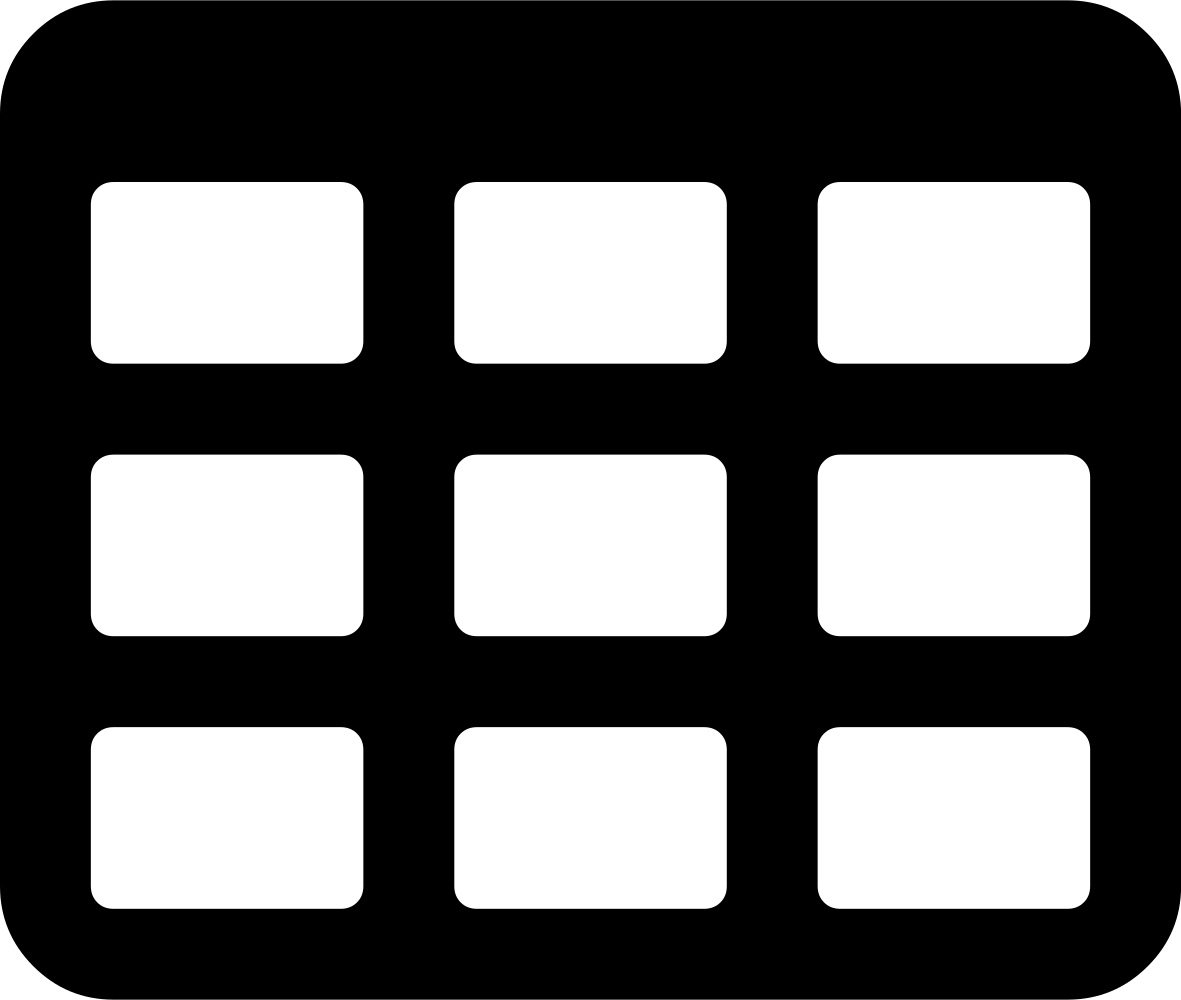
\includegraphics[width=12cm]{figures/view_data.pdf}
\caption[The GUI's data viewing windows.]{The GUI's data viewing windows.
Top left: the Tao root window and the menu shortcut for viewing data.
Top middle: The d2_data_array window, which list the currently defined d2_data_arrays for each universe.
This window also includes links to view and edit (see section \ref{s:gui.data.edit}) existing d1_data_arrays.
Bottom left: The d1_data_array window (in this case for orbit.x), showing all of the datums in the array orbit.x.
Bottom right: The individual datum window (in this case for orbit.x[34]) displaying detailed datum properties and allowing the user to edit some of these properties.
Top right: The bulk edit window (in this case for orbit.x) providing controls to quickly edit a few key properties for multiple datums in a d1_data_array.}
\label{fig:gui.data.view}
\end{figure}

Figure \ref{fig:gui.data.view} shows the various windows that the GUI provides for viewing data and making minor changes to data arrays.
The d2_data_array window (top middle in Figure \ref{fig:gui.data.view}) displays all data arrays for a given universe.
To view any existing d1_data_array, click on its "View" button.
This window also provides the ability to edit any existing data array in detail (see Section \ref{s:gui.data.edit}), as well as functionality for writing existing data to a namelist (see Section \ref{s:gui.namelist}).

The d1_data_array window (bottom left in Figure \ref{fig:gui.data.view}) allows the user to view an existing d1_data_array.
This window displays important properties of each datum in the array, such as element name, meas, model, and design values, and weight, in a scrollable table.
To view a datum in detail, double click on its row in the d1_data_array window.
This will open the individual datum window for that datum, displaying all of its properties and allowing some of them to be editted.

The d1_data_array window also allows the user to edit a few key properties of the datums in the array all at once using the bulk settings window (top right in Figure \ref{fig:gui.data.view}).
This window is accessed by clicking on the "Bulk fill" button in the d1_data_array window.
From here, the meas_value, good_user, and weight settings for the datums in the array can be edited in bulk.
Changes may be applied to every datum in the array, or to only a specific range of datums using the range specifier.
Once the desired settings have been specified, clicking the "Fill and apply" button will edit the d1_data_array as necessary, and changes will be reflected in the d1_data_array window.

%-----------------------------------------------------------------
\section{Creating and Editing Data}
\label{s:gui.data.edit}

\begin{figure}
\centering
\includegraphics[width=12cm]{figures/create_d2.pdf}
\caption[Data creation window.]{Left: the data creation window can be accessed from the root window's menubar. \\
Right: The first pane of the data creation window.}
\label{fig:gui.create.data.d2}
\end{figure}

\tao data structures can be defined via an initialization file or on-the-fly via the GUI. For setting up a data
initialization file, see the \vn{Tao Initialization} chapter in the \tao manual. To initialize data via the GUI,
open the \vn{New D2 Data} window 

The GUI also supports the creation of data arrays on the fly through the create dat window.
This window can be accessed as shown in figure \ref{fig:gui.create.data.d2}.
In the first pane of the data creation window, the user can input the desired settings for the new d2_data_array.
The user can also select and existing d2_data_array to clone.
This will copy the d2 properties of that array, as well as the d1 properties and all of the datums for each d1 array.
Once this information has been input, the user can hit the "Next" button to go to the d1_data_array pane.

\begin{figure}
\centering
\includegraphics[width=12cm]{figures/create_d1.pdf}
\caption[The d1_array pane of the data creation window.]{The d1_array pane of the data creation window. Top left: Here, only one d1_array has been created (called my_d1), its default data type has been set to alpha.a, and the start and end indices have been set to 1 and 12 respectively.  \\
Bottom left: the lattice browser for the ele_names that will be used with my_d1.
Right: Here, the user has defined three d1_arrays: x, y, and z.
The data type for new_data_array.x has been set to velocity.x, and the start and end indices have been set to 1 and 12.
Here, the user is currently editing new_data_array.x[3], where the meas value has been set to 0.2 and the ref value has been set to 0.4.}
\label{fig:gui.create.data.d1}
\end{figure}

The d1_array pane of the data creation window is where most of the data array's properties are set.
This pane is shown in Figure \ref{fig:gui.create.data.d1}.
The d1_array pane of the data creation window displays each d1_array in its own tab.
To add a tab, click on the "+" tab at the top of the window.
Tabs can also be removed by navigating to them and then clicking on their delete button.
An existing tab can also be duplicated by clicking on the duplicate button right under the delete button.
This may be useful if you want to define several d1_arrays with many of the same properties, but want them each to have a different data type, for example.

The next section of the window holds the d1-level settings for the array.
Here, the d1 name, start index, and end index can be set, as well as the default data_source, data_type, merit type, weight, and good user value for the d1_array.

The next section allows the users to set the ele_name, ele_start_name, and ele_ref_name for the d1_array en-masse.
Clicking on these buttons will bring up the lattice browser window (bottom left in Figure \ref{fig:gui.create.data.d1}).
This window is essentially identical to the main lattice window for the GUI (see Section \ref{s:gui.lat}), with a few additions.
Towards the top right of the window, the user can specify which indices to read the element names into.
Clicking "Apply Element Names" will then write the ele names that are currently in the table sequentially into the d1_array's datums.
In the example shown in Figure \ref{fig:gui.create.data.d1}, new_data_array.my_d1[1]|ele_name will be set to "Q00W\#1", new_data_array.my_d1[2]|ele_name will be set to "Q01W", and so on.
If there are more elements in the table than there are datums to write to, the table will be truncated and only the first elements in the table will be used.
If there are less elements in the table than there are datums to write to, the elements in the table will be looped through so that each datum gets an element name.

The bottom portion of the d1_array pane of the data creation window allows the user to set the properties of the individual datums in the array.
Once a start and end index have been specified, the "Datum" drop down menu will be populated with all of the datum indices.
Selecting an index will bring up the datum settings for that datum, as shown in the right of Figure \ref{fig:gui.create.data.d1}.
Note that any settings that have a d1-level default value are automatically filled in.
Once the user edits a property of a datum, that property will no longer be auto-filled from the d1-level default settings, even if those default values are subsequently edited.
If the user wants to explicitly fill a d1 setting to that d1_array's datums, they may do so with the corresponding "Fill to datums" button.

Once all of the data settings have been adjusted as necessary, the user must click the "Create" button to create the d2_array in Tao.  Doing so will close the data creation window.

\begin{figure}
\centering
\includegraphics[width=12cm]{figures/edit_data.pdf}
\caption{Editting an existing d2_data_array.}
\label{fig:gui.edit.data}
\end{figure}

The data creation window can also be accessed from the d2_data window discussed in Section \ref{s:gui.data.view}.
Clicking on the "Edit" button for any d2 array will load that array into the data creation window, just as if the user had cloned that array from the d2 pane of the data creation window.
This is shown in Figure \ref{fig:gui.edit.data}
Note that any changes made in the data creation window will not take effect in Tao until the user clicks the "Create" button.
For example, clicking the delete button for the orbit.x array would not actually delete the array in Tao until the user clicks "Create".



\chapter{The \texttt{report} command}



\newcommand{\CESMD}[1]{\texttt{#1}}

\begin{document}\thispagestyle{empty}
\begin{center}
\includegraphicsembedded[width=0.6\textwidth]{%
iVBORw0KGgoAAAANSUhEUgAAAsoAAABqCAYAAAClFXeHAAAAAXNSR0IArs4c6QAAAIRlWElmTU0AKgAAAAgABQESAAMAAAABAAEAAAEaAAUAAAABAAAASgEbAAUAAAABAAAAUgEoAAMAAAABAAIAAIdpAAQAAAABAAAAWgAAAAAAAACQAAAAAQAAAJAAAAABAAOgAQADAAAAAQABAACgAgAEAAAAAQAAAsqgAwAEAAAAAQAAAGoAAAAAUmzrsgAAAAlwSFlzAAAWJQAAFiUBSVIk8AAAQABJREFUeAHsnQl8VcX1x8+972UDEkBERQFRcUWWJICiteJSLWprrQbrhpAAotb+61Z3jVq12latuywBsWpdWlu1al1xRZCERXBhXxRQRCQBkrzl3v/33JeXvJe8kB2SMPPJzbvLrL87d+Y3Z86cETHOIGAQMAgYBAwCBgGDgEHAIGAQMAgYBAwCBgGDgEHAIGAQMAgYBAwCBgGDgEHAIGAQMAgYBAwCBgGDgEHAIGAQMAgYBAwCBgGDgEHAIGAQMAgYBAwCBgGDgEHAIGAQMAgYBAwCBgGDgEHAIGAQMAgYBAwCBgGDgEHAIGAQMAgYBAwCBgGDgEHAIGAQMAgYBFoBAlYryEObzsLll1+e1rlz56Mdx9nPtu3NPp/v05tuumlFmy6UybxBwCBgEDAIGAQMAgYBg4AYotyESpCfn++3LOsaohjiuu46ztP5LeV6Es9mNyHq1hW0z+hU6eobKuIulbkFa1tX5kxuDAIGAYOAQcAgYBAwCLQMAnbLRLvLxDocYnwmx2RK/Fd+H+C3nONX1113Xfd2g8Ju1oliubeL7Z4i2eM7tJtymYIYBAwCBgGDgEHAIGAQ2A4C/u08M4/qRuA0vBQedthhr40cOTKs3pEk9+Hn5JSUlH343XDbbbddi1rG0Zy3Fay/DQaDN91xxx1ryLPIwFEHiSsXMvcwTFyruziB+ZSykMPxnpt/BgGDgEHAIGAQMAgYBNopAm2FvLVW+H1kzBclyZpJSHEYXeXK/CJlnoVKxrfcqLpZ+bRVnmxJT08v9nKmKhe2/QtI8olcJ3EcLJZ1ufRffKl8JptaZe5NpgwCBgGDgEHAIGAQMAg0EwKGKDcBSL/f/1QoFHoGKfKJHG/dcMMN+0CSf0mUSiJXa9QQ5Q/4+Wjjxo1tQh+8W7du7jXXXBO89tprRbq6R0OSLyL/XbQsOBuinCP+tJc4f5bD1ZvGGQQMAgYBg4BBwCBgEGiPCLQJ8tZagR8/fnxSz549L0OK/EfyuJkjFenxR5Dlq7F88UVrzXe98pWZt69Yzt1w47O9JZ+us1LE6krYzhxljAB6y9ypG+oVl/FkEDAIGAQMAgYBg4BBoA0iYIhyM7w0pMl7EM3QcDi87vbbby/ivG1LWvteliIZW8+hHFMhx/r3Ksc1kOOrKdk5SJWT+H1Diqac3AzwmSgMAgYBg4BBwCBgEDAItEoEVMfWuEYgADnu0L17d+fzzz93Z8yYsZXzZXvuuec6zts2SZZ8W3ptzMLKxeNi2Rlw/vXiOvdJ0b7vyF4/fgVJ/glw7SW2v6/0GLRE1s1d2Aj4TBCDgEHAIGAQMAgYBAwCrR6BtrLArFUB+fjjjyehe3x7v3799tOM3X333emHH374iUiUh7SqjDYmMwPX9xC/eyWL+PaBLJdxvCKWf74MWJaGqsXnEOXJSJc3iRNi5aIUyMALD2tMMiaMQcAgYBAwCBgEDAIGgdaOgCHKjXhD69evPwtd5NHoIqdo8OLi4i4Q5zPYle+YRkTXeoL0y0mWpOBpqFX8GjULh98PxbaeRVf5KElKysQknC2/6PUYuhiv88yBRKeIz/cn6X+u6i4bZxAwCBgEDAIGAYOAQaBdIWCIcgNfJyoXhxAkn+Omm2++eVEDg7du78npAyDIN5BJP0SYHfjcp8Xxz8N+stqBPkMyV3WTfOwn2+5NXC+rKMwJkpR6oUeiK26YH4OAQaANIpCT45Mho/eSg3PTW2/uGaxnn99DhuXt1nrzaHJmEDAItCcEjHm4BrxNSLKaSbsJ6fECfpGstiM3LCdNyt2bIcW9KNVW1CteEivpWfElpUko7EKcz0Qd4x0Znv8/mZG/XLLG3IZkeQp+0zj+T7JXz5FCJNDGNRyBARd0FLdTsiSHHSnbVCqLng9sN5Lh+X5ZtzpNvpqyhXfQxnXit1vSyEMlRTOn/FAPn8ZLYxDIHo8lm+AhstTKRLWqv3QKv0k0/25MVC0W5mjIe5l7mLirB4qTNIi2ajFp3d9i6ZmIDQIGAYNABQKGKDegKqBucTbe94Moj4U0t6+d6QLpl0COT4EQhykjAwH7ISmcuC2yZbVyMWtfpM1ny+bVc7lYK0VT/y5ZuT/lfBzH3oS7UjLHfGVMxoFGXU4ldys7ZknIPhSpfW8WTSIdC6SwaNKR5E4l4Pod+K9Gcr9Y5vT6HGl9fF0rXtNHOsgIGTCqgDe1tdbkssf3QJd8J1m2cYNS0qlYlj6oW7o33mWP7i8B9xKknH+QrwpKGh9RLSH7QcKT3dRantZ9W/Ht0O0HmXlfqeh7XdxtL5FtvD5/wwcwGsYJhvjOgtIjvVReayJ2deV+4Kh9xJd8BHXkKL59tZk+FKJs8y1rnWodRHnImF4SsoZikFJ3Bj2KfB1JHqnTrg7KDVGu6x2b5wYBg0CTETBEuZ4QQoyPhCCfSxs9iS2rv6pnsLbhLWv0kXSOqnKhVlC+p6N+UOZOrmYH2uv3jxa/T/WRUcvAuZJP53okZ/05jqUDgzTn/6kGsVO/xkUQyBp9jCy3zmLgkc2NvmC2J0cFOsCvp64LuXS+EUeWS/aaBRLO+wC5/fueVFWlzyKjPdw7Jj/Fee1E2Q3diz/dUTGxs3iDrpdi4uf1uVtbHK61UtK3PkkU8+sTTa1+HPsqZjJGSUdnDX7urNVfYx+kuGoGcTBHB45kDq3o8QMTblRzuvEOhJL35PeFpWzzgzyfKV9ndBY7eI/3GVkW5NvVt1kzrloxC6H3b3NIUL7dViqZuaWsEdgojvud+JxlpPmlfDpVcWi803UIyemHsnXQCUQC+XSwcCP7UvF8XqQuxdc87Ew3nB1BSywWCdvHS9jV9iWLt7JfTJbIn7Vz8xiTGXNqEDAItG8EDFGux/u97rrruuFNd6ibX15e/mrsltX1CN66vfTL6USHBLnVzUTcAJ3mM5KyJbE0yYJIOMEqvfa5BWslK08J9tOE7UpHfm6FCsYbrbvQOyN3SBuz0q8gZSVm6IJDTCwWTKr03nEXIj2GEEEHbHd33sVBvIfD+d2fO8Pxd5qUy2IkzUu5n47/0/idV49S5OAnQoA8z/A2pW6xrvq1EqUaLkG4Gn5iw+HfdjElaH+At8YT5cwx3cnvTyBzmtpVqP3cg9oP5laa0dnWp2D8jUgY2+B2H7A+BciGV6RZW0JvQJJfo5Dr2LM+JGF7TcRjcalI+r88kC2nqzgW0k8k/2LtzfdRFVflaSyunMe5Ck+uu404isWxN1Bn1kOeC8VnPSdzpujMTsOcSryXpx9N3m8lT3uQpd78ojpVmaGGxdcSvlWtaPOaHN7DWPKl9ukPoPwJBnsJK2pL5MjEaRAwCOziCBiiXI8KkJKSoioXu2HlYuKSJUu+r0eQtuMlJeNaOqRhFZ3lYvHZ98nM5+nw6+lCgXfQY34YkqwbkhzIcaEMG7VIZk6HfBjnIaAbuHTecgd8ZBTX3T1eYrEY0pG/QChnQ7Z+QMJXJn6m3gOqBuB24RpVF/kF5+dCFA4iHIfLe0H8bAl+6qWbHEOSvVSxia369dYG4tDdFcv59Viol0/XDRH9xfgk/hhnOYsgae/hV9Vyok7tniTjvyNZ2Y+bg/GjeeeUw1UJravS78Y7y/4/4tjTi8Cyu0rJmtM4TzyIa2wqc6bMrgyq0np/CuYQ5WLKdRn4VD6KOZkoEnpYUkqX1PhOIt/NPz2/2eOTILeviS+wnOvfcvSIiSNy6jrvgdMq3scq3vdG0tvGQZts9UCSPABPwznQH/ak3XuBs87cHImU9XgI83PSt+R+ef752HfC4+245593JPvC1SJ8r25oLZL6gxh0/Z4QDMpaiZtBrRoU/pJB1v1g8B3560PO7uFgsGGcQcAgYBDY8QgYolwH5qhc6AYbp6Ny8QJbVc9/viEdUx1x7/THg3NH0C1dQD6U8MBJnKtk9qSVIpPrn7UFT26TrLFP0MEfRxzoOKLnXO6bL31H/E2WvlZe/4jasc/OW5G6W2MoIbrI4CxKVp0xYid96emB1yz6KvRdF8oXnWdJUugf2LG+nzCQGaR/ldxNp/U1rlrcoNFdYp5sxu/jvKOnecebISEBpvIdKWfxoC9Gl7aDVSalMppw8UTZlbnic/8kIch1rAunWBBBP/kjXwH01O2xZEkHA+o6kF6nyGkj/vfLT2bh1jHEB+HGRaTKt3PWvETZi7zi34InVY3lC8nM+ysk7TISjX2q55sY2MyQOfsvrFO9qHBiEP/fyNBLH5dQaRbnZ2oE8c6+UGxfQMKBUgmGg7IbahzlXS0p3ZRC+un47cXQ5He8u19x7pmi5DcdTIbwu58s69RLhuVcV4Ow87AW50rhtpWS3XW1FE4LyoALisSfzO6aWrdai8unTo6fJ+l7z43MHuTPZJZKBy0MNLSRMs4gYBAwCOxYBAxR3g7eFSoX5+NlKTaSX7/xxhtZpdNO3NBR3eiEf08nycYiaFO4zp8lY8XbdEY12EEdJXYlo+cSKV5zC/5UmgZBQwUjvUcR52/VEbb9P87KHUknfy6YoNqC83iydaYUFizjqnasIwOyb0Vyvpd+GcdCk54j8AnbC+LFH/3nY/fESOxbebd3iZ38oBSxOLMulzUGCXM1PuKqtHvL9/Lp9mYa8lfI4V8vliSXTWkg1eIqwW28RDlp9TjiOIS8xGZmPySiB0jhE4pdy7lAykZJiR8TVCQ2Txzf4jpJcmzOZj+8EQsxOlDRtxFbFpG5U1bFeo051xmdH0nnGzl69WdSai3l+hrwiLbXGk93osuVsk5IoVlfoHrP9XJIoAsrZgZ0YJCV1/oGs5FBRkVpIM5O7kKqwSBuRAcL9Sqp8WQQMAgYBJoDARiScbUhkJqaehrP+nI8C0leU5u/Nnk/6L+KrnUYefcx9f8NUsEbZMaMUKPKonqjTvgTCOFfPdItMpCOeyTTw7v2dKlOv1tyKoSmD7iiMuHjR86ToilKfOpPbBZhGi0UPJ0gS6pzLY0woQtDlCNpfC5zp91di+Q6YdDG3YTQLJz8LTrsf6dkU6gH6L5WSIMbE6HqJouFvnacQ3LtmxR3p+UuwgmiXoW2LIOXBjq3wYPPigTA9CMsfRRNuZFXie5zDafS5TwZPGZCjSf1vuEE8MrgqBU72/qS3FVrm+IGUK048yZrBgGDQFtHwBDlWt7gbbfdlo2ViwtRt3ht0aJFH9XirW3eHpQHeWP3PZ3GtSFvln0KREqnihvv5k37kXheQHo5J0LmWIxju6djXi7BQpzGJ9OmQobDv6ocjGjGvb592xuNKoNK/6zwCAhT/Qi234dOK0sA7ZQLGpVeYwPNRzfdZ79MNnVhqI4M4qWo9Yl30NifEaw/Iau3T3p9aIvXKV+JYoxEt4bbikm/hKLmGj6b+0ZRwdnxwvVoAizKcxiYHnFeRvROw35tnWWoRkIbFkOL+7bcTaSRaODS4kmbBAwCBgGDQPWOyCACAnfeeWc3CLJaDPiWBXxPtSu9ZN15y+eOhoSopByryc5tUtQTnctmcEWTFxDjn5hl/sFjha51iYTDQ0mm4WSpGbKz06Ow2SBBF2bFuvSULbGXDTr3h7B8IE9GCFMdUkrH6YFfR/b7fkWD0mgOz6HwBsr9Ja+d957fwHefb4sd/iX182Av/zXz05nZi9tr3m7GO0lpEGW3hDJUjzSIPvHOI5WWdWNCsmxZv5ZQ6hnVM1vPax0gt26JcthC6l19fFjPAWM9QTDeDAIGAYNAbQgYolwNGRbvJZeVlQ3n9pEs4Cvgen01L233Uq0vhOxx9DknUgh997MlNTixQTqXdZU+KaTr1qfhTXUfD4drnCdDxkQsF9QVtr09t3TXQldt81a5H6stlKt6UvfZrKeKJWz9GWktxKaOwYdloyvuLsMqAiRjBzvLWslg6WNSDUrOohpsc7u5yVyleslq4UP1cT+h/kBY41wacf+CRWyq2tFyrjZ4w4GGlac5c+ja90Q+2xqR7o51iOpqKjU81XKj9RNlS+2K1zEwrKVw5rZBwCBgEGgqAoYoxyAIKVY8DkOKPJrftxYuXPhOzOM2fkrZumw9HonUWRSkCwRkvdhIk1P2b7jO5faQmD19I49fgOjM5pfNE9w8yPmpoiR9V3OOQPZ0pWSFUyGYz3d09LJRv3ZYJdKLObZP2Fx3Hl7ubVQaTQ3Uefl3RPEcA7LZ8ny/6qLA7cVOmexf4CGK0R+JYyZHvMTTlW5SloHO9i7mCifWLs22a2P2dWGEScDWLlG2VKJMLTDOIGAQMAjsBASqOvGdkHgrTFL1/FTlQhvmye1K5SJzTS82QDiXcqkpKPQs3clSnjaz2TdwIHKZWwC5sZ7g7BsOTM+xWURG6cH6aJdyno3imCniiImzu2XQ6D5NwEF1Z1/m8FYG1hpPUcGLUlQwrdbnLflAF4UWFrxLPXirQbMVA8ZigcWrn2ot4zPGGCupp3dzL95ahyV7MAAbI8OHq9TZOG/Q1I6b8rBRTzaV3CBgENh5CLTj1rVhoFZIk49H3eI4Qj7crlQu+l3SCcJxJuRCpXD6zj8SN/y8fPZoogVLDQOuNt926X8gOP/lMYvQrENY5Hcli7A61Oa9Xd53LTXzpVPbFU6FYlY/Nnq4TbJHo2LQCDevTzGytXcbEbL1B/GFj6GeqlqQugKI8iopmvoO9XZV5Fblfwt/vaW4j1ptMQ4wWpVQOHt8Z771HpI9qrd36LqIZv/2a7V6YcmwvN1IrzcqX7347WwqiEHAIGAQaAoCRiJThV5vTn+PpYuX+J1RdbuNn+m2tUtLsyGreZA0NjFwV3L+uJSVqsmllpvOLHzmexmcNxV92oEcR7CBwig2pfiQNCe1cUTrn33LXQHE34O71q2Ii0iVsURhp0t27qNIXt+IPqrfbz52ZdldzbZnM+SJIeH1C91qffW/mC3QA2zMwU58lqyAJM+TORN1oAEHtO7j3uT4vFv7getvuKd1quXqcXyiO/dqeL5PSnSSpoYLM4NTu1pGDe8tcCMzb1/alWy+9QPFCe3N+0pHzTyVV8O7YcDohn7AXOQa6uxX4i//RFTfvjnd8NGpssXH1vCYvCwnD1a4K1uLo7IT3Eg7tJQFoHOkaNonzZmkicsgYBDYNRAwRLnqPV/H6Q/l5eVT7rrrrnidyCo/be9saboSjwlk/DD6rDI6s2eZtX9XFu2ARV66PXBmHgTH3Z/0WdBn3yoDct+XBQVftT0gG5Fjn/s2i+90R7aeHPGzN678knv7sxlFPyyDPCdqVq2+znVWYq1kkiStiRDJ+oZrzf78ZZAcS61d6NYZ/4HYLCK7EQI8t2CKZOXezzUzI5VOdd77sSvkIVI0+YvKu+35ZPOacxhw1iyh6y7EvrTiteOdDsSXdGKXSTmNWSPsp7v7QowZHLI1t5dVix0b2X7aU9V32PxGlkswZQ7twjQ2XHm/WTKskutiH4Mmb8ZsEOmzK2Q0Zj47bffELiLN18QOTpfC6aujT82vQcAgYBCoC4H4zrsu3+30+c0333weRTspGAzeCUnGtFU7cQMu6EhnNZLSnA5B1kJ9iGm4Z7CZrAvudoxzw/8iD0hN1a4uptL88kDzT8PumKI0OJVPp64hDPrEVqIFk/rtDeDZDSzw+yvSthHSLye5XmmoTeUFT65o9AYx9UpkB3rqgzTQstRCyoGkqnVzDvrNSraqnCX3VV1Ung3EvK4u/kvAHiv9tJ8Ty70NMpqgPPZM6ejseGnpCBboLkv/C+T9VogpbYwOCO2HeR2juHcppPm3nOfxblmU6ei3oLrn/TnG8Ow+GZiH6cgmugG5mBH03UL7chUxHcWBepey5JjDFSTb+sy9RsR/O4MrvjvjDAIGAYNA/RDY5Ykyush9sHJxL7rJ9yxevLiwfrAl9oXt5VbUYedjj9Z3GJ3U7+is2NHMXc75VOnQu0pSl7gY279r+SplNdv3WPFUNyIJ+/7I1QpvFlYwTeeG6UB3EedP+ycd9OuUFqlWQteN93MGJOM+Sel0D7rLEInGWjBIGH/Tb7Z0K5Hh6wuvuRAc9Pt5neKjTlHNHFjYuZdn1VVNuuDvcMkc01jTaE3HZkfFkJWn5e+TILlPUTN4xtvBL8HDum9Vw7nuAFU+vt36Vy7GceztEVPXnQ4hxi77lNdFZ5MKp87yzpOp2678GX9rqwJLFhsSQaqb4AZO2IedEm+jDpzN0Z2DyKJHgngtZiRcweqPcx1k+dAEPswtg4BBwCBQA4GW7gJrJNiablQs4NPG/hN0k59oV1YuBixLQ4/1ZsjpfnQMOkX/uvg7vNIiVi7qeqnzJy3Gy80cSnRs+rIJSFAH1xWsXTyf/fBGCbi3UJa3OWpbvq+S5IPhibmoxUxHd/laOWLsnu2i/HUWggGdz+1FnUA/GdvbliyUvsVf1wimAy7XejVChGKeunIcW4OfzB1lSO3TZY25ASJK3ajhVEo7SYrT1RTjjnWD8hjYiKoVqZRYeTLGEMN/kLlTa87IzWQLdtsPiWawHOssyWaQc2zsrQacdxV/4Bri/AWvfiME/XHauVzau9O5N4p7jxDX5gTxdaCmnEqGR4vOuBlnEDAIGATqQGCXJspIkS8CnyHbtm27FNK8rQ6s6nyMZNqt09OO8pCUpHrJJ0WSsxaI49wvsx5s+gIaN9w4QlLU+wXy8u8In8FigSV3i0657wpuISoY5bqYEdvC2+Nzri6A0sWP1nUScl5CupwjqgO6s12i2f7mytPA5T0qZj0op/se56+wSUriAYXrv7oGfJbsA2YHSt8R9VNbaa5874h4dIFcVt6T1BlVK6hmvcH9DnKYLymd/y5LHyxvfHYaOXthuzmkuUdlupblSMSGeuWtuJPCiUpav+SIzau2JWPi/NXvgnCuzkKcT314haE3W8W710pxp6el8/JXJVD8LIOn69H9P5rnH0YmKmIi1u9M3PPF7x8Zc9ecGgQMAgaBhAjsskT59ttvV7u+V0OWr7znnntqSrASwtVGbmafr9sX55NbJQ9rIV73y7xpS3Zu7rHWUFRyDh3aD+RNyd9g2c1/7c7N0w5MfRFStblTzmOTl8siqdY63tAHEGYZIq79jCxN/59kX3jADszpjk3Kj/WP6IDOtZZJp15KphI7Zxt1WVZXG2xYEKVfSuce6KC2A9d3RIpkjT6GxYsPo33yMYTuXEqFiglONVM87RTrbVQOjpO5fabJzPt0tmjHusjgTU09xvQf9VA7szyzhvFSXts6shGZVyCARv6OzvF5qHnMo3370RswqA1vXaisxHz+E4skGPw5AwrUU/SzinWuDtAGy0/O7Rp715wbBAwCBoHqCMQ0dNUftd9r1CyscDj8R34/5PhPuyupm6zT/J04dCr7PQjaP1pHGZEUWvavKvKSwVTpeZI9RqfcdxGHPuicqQ9JqLxXpPPW8UKtTnt2H4uiThA7dakMzn2I6+q9fa2B28SDfjlaR8dBWGiH3M/EF35xu6pBCw4ohZqdi0pRfPFcGQRpOozNTao9iPfW6q6y8l5AzeZppMYvcrwl2XnLJKNHmdhJ7/OdXEJ+9+ZAVUmLxat3nH9J0DkSvd8TZdbUzxu0mUtLF96qx2yabZHnapvHON5Cu4bmzmHwX8SCz99BiFWdq/aZPF34WjR1KAN09RfjYM6unCHbUn8Wc9OcGgQMAgaBGgi0rY6lRvYbd+OWW265BILcm9B/QuWiWgPauDhbTSjVZ7RsXaiinccyJC5Xtpq8aUaKJn9Ap/VERZ4OQGp6xy63KcCCp76WvluGYQLtYnBYBwkKVeBR80fN0Iapog5WBLLyVmJO7mQZnu+v6bEN3unUuQvv//cMGsi8+7l0Wvnu9kvBrIQVXob/knh/Hk/6iQz9et/4+639yj2Vr/TXlH0Ex9F8F728HDtonkStWyhJdtxzIMcW+r9nygIWyO1s56nGWCvIhpp705cXIo+f1pmtgPWj5zfWY2OHfpa39XZsTNs/d9hIyhtwxHnbnfzvFnfHXBgEDAIGgWoI7HJEGWKchS7xrzkmgsVyDq+XrYZL27zMHo901ro60snSKVlOPhIXiFgzuoZavUicNHl01fqGxfTyUJjgJZDlpMRe2+ldJRtzCx4Ty69Tz1oX13IEai+tVlMd3FnPSfHXN3q7j9XuuXmftEQrodtPB9yTIC8a+3okhDPqZe7O35Wpe/fOBKQnR4Lh7DYlVQ7LKciL0ZO1mGVxVc/2L2CRQJXCObrVmVQc7JvA1/tHjlfJ80PSufdPt1PpLG/hXLKrKiTValMNnYjtRBP7qIHNts+HrWlnVWwMnNPmWLvLsJy0avfNpUHAIGAQqESgfUimKouz/ZPrrruuGz7GcXyFRPl/kOay7YdoQ08zx3QXJ/hXOq4Mj0S47r8lvc+LrbIEnffdJD+uuRGS/AQECYkO22vbzkxIzvscKqHadVzhxNUyfPSVstl+hXendXMYB6auPD3uRDioysrlLA7sIgMm3CkLHvsukadWf6/kICwOhO6EHGpWv0BqzqK1ejjVyc0a+x9IDzMnnnpRNJCqqQyWfmvekUXyQ/Rmq/6dX/BuXP6yxq7m3R7CvV9yRPRyVLJs+3/LznYfcO+5OP8782Kip/Lwp+1mQfWtO+zTXXxOL0zBHY3UGem5t/lOTLAd9rlvQ8XnHojxw5XSes2F5faXUHoPzpbHZMqcGgQMAgaBSgR2GaIMKU5m4d5ZFSoXd4OASvDah1PrEbZ9MbJxNbnGZKa7GEnlDdvV99yZJZ+RH5L+F78ndmA6eVVdzGwJu+Mke+1yKdTFWruYmzFNB2yvQXwLMXml1gSUUOi71IVuiSanIcvueeILrkPS+CCzBtvw17acGx4GccEEnrdb5GpJS+nKzmm711kIGzve4UAnwjKwsn9G+Ngg4yQp/E9ubOKIexDrqdWe6w6DmbmTIPwHMYDoV5lPF1UMkSdlyOjF8um0eZX3m+VE7Sg3M1QqoQ107Ev2+kP8Tyb6E1Ed8vHOviYtVTPSRcY71hVODLGV9ZwERe3FVtdmQd+OfRsmNYNAm0JglyHKLN4b6PP5Tkbl4rW0tLTCq6++utlFGTttw5Fu9k+pdefRCeniqG3sVPU7KWpmlYvmrtafPbpJBo57UOxwJh0oZpyYhpfgLKZop7Dr3NbmTq5NxBeRDj+MWbi3xbFZtGb9AsI0gLzbCfIPqXR+g5SukGdvczQz24lNMVHysc8bc+7eUTEGCFPGvSSo6hT1iEd5lu3TwWACssXshA+p8vDRn0lk8FGPCFuZl7m9sXKyqg/Y3EzO9qrKnZUMoXuMAeYI0W+nNTodsHezB0sASxauexpZHMA73UBZkIa7M6jTC/jen+C+kugd71wfai01mn1IcqjDjs+MSdEgYBBoKwjsEkQZabJ2OOdwbITMvgJJblYi1qFDh1AgENgICUd/cge7ARfsR0d0CR3TfhBOEncflcJJ/2uxXDTWjnKiDG1NXSUZpQ/SeR1IGfaA6l0gvtT5qF/Qse5iKhix+BRO+5LLm5GwYldYB0DeUZMYWtZAno+Qo3NnNX5nttiEazl3apCLWjzW83bmmMPwOZC66pJ/H+99ONdaeevpvDGBSkJ1IW5SZSBPjcO6TH7wvcw9pJdt0VHvgxf8U/xJmZTvfGCp0J/VMltHSFLgJk6uaL6SNdKOcvUMDMz9ifgtpMcsUBRvcPcFXlCtct+WYMpHHrnPHo+KA/aWI+o2FTE0dhDWYN1m6loowOLR+Jy7OgjVgZdxBgGDgEEgMQLtnihDknVTC6SVcijHX7F4sYp7nDafQ0L9Y1lZ2QvJyclbmi/WesTU97IU8W09n47nJ3RASfx+iD6gLghqG043Ssgc8w461U/RuV5GpgfTj45GBWNFu1DBGDKmF5LSVPlR1shKT72iYe9l7pS32aFvIXF8Bj63EVhnDGIdJq6sIVIa1mn6T2IftOpzS1S3VXVwiyEu11O2EHU3Qlasii2Vo9fRglS/r9eWOwSSnYuXKqJj+Q6VlPAhDLTWttnB1oInv5PBox4Vxw9ZRi2psnzeAOFSBlALMflYEIVmp/4OGb2XOL4xmK47g2wOIS9beRuP8D7/TZNU6NkzjmbQCWHzuupVRW/vsF/HQofFw7AqSVstd4S3s4i2yqs5MwgYBHZNBNo7UdZW+SCOM9BPfic9Pf0jfqu1lE1/8VdccYWuVJ/b9JgaGEPnbSfS7qtOqy6I2wj3+KN8OuVbkWkNjKgO72pxNIpa81i9qEpQt7wdMno608qqYnAC5IeFTOGPZNjlT+2UzRSqctb0M0eOR3d8qOxm3ScrZWmjIpw1+VvJz/+bvLQKPWT7Id5ztW/WzWIm4XDinsURfUuNSmqHBBqWt5uUuyeTloqp52Eu8OFGp5uduwJSpjqwPSvj0MVvjlzPYOtjBlttT3c7WpA50+ey8QiDI9QtIvaUo0+S+Eaug0gvlDnTZ0dv7pRftYEetq4h7VOog50gx5sYuP2fpCb9Tz6ubZFp9SrazLMVdQGhPUJsFlxdq+LfXFcw89wgYBDYdRGo1um2LyCQHHenRKMgx6Us4nuqgtA2ayFJoxPqHOegdnEEESthfo3jHe6XNWtC1SMbOIoFP3Iht5GeeRK1hyQt/DGnsd1A9VCt83rb1s8lLf0ZynNwhPQ4V0rgxyJ6NAYfbbA8UZRd2ZNTbOU6z/G7jKNx7yaf6fgBF/xdfMmDkciNhZBEU9DfjhxdsK3sa7WLN2NzG1DdZG8xF9+Ke2vsowafO9QP23qRcL/lqBBVKjbYzHXC+u2v4mi7LmPla1K8/yQKcBWHvmd1Ws59GS9dR504f6fp80c2CtKZgeN4j9qPwHjdUdK35LVatyDH0051djJqPqqtE/P9WGyrHUhav1PzZRI3CBgEWjUC6Ge1TwdRVSsXx1K6IyHJE7lGctC8TtMgxlshyWdBlpUIbSHN3/F7Ps9Smze1mNiGXZ4mfv9pNPg/4y4SJutVrFz8Az3VllH9UE3SqGtOHeVonLrlbCmEx5X/kBIDDAvCbF8tg8Z0jnpps78u5vpsew+PyDalEAue3MZCqAcgyeU1olE9yw2L2sK3zNyE+wsv/5Z8Lwdsea9GWRpyY+7U76kzqKVItXpPdbXcWxoSVav0q9sxW/77KKNauogVvSZxfYIkJd3U9Hw3YiB6cC5brKu9dq99jQhbLPdZdsB7ZceR5PjRYj1woO6Ftb2Ocd5GP6vks0d+jLlpTg0CBgGDQBwCbaFzjctwfS+CweCeEOSL8f/KokWL1AZpS7jDSAPCKtdBlh8sLS39E9f/5vqnXB/cEgl6cQY2s6rcGs95F4jlt5xP4bzxEssWy2gDIl405Qfx+SZDClSFAIdtZcv3c06qSLp3v4390zVHrnuYlC5p6sp6xGDJ64BjeU1IIDupXWPEZK0Uo+y8a8n77p6db8f6QzOQKoZw/nco7RtxJY7sajda+uVUI0ZxvtrGReHEzeJ3ziKzOltV5VxMB7pyNjalWfC3g11HR9cTqPpMBF/9Qn1hvde6nRVOi8+gu4XhB2oXjRgsxEdkrgwCBoF2jEC7VL1AmmtDWFkkhDXPjh0ffN7bcrX53yJk+KdIkpeTHmoCEXfTTTcVYobuGNLvzZ35PLub3xM5VAq0PVed6EQJYgqBTiaelV7gzDymXd0JsK+DPSsXjjuRtVDvyLxpOqfYtt2nk+ZhR/afFOIQ6PGe9F9TsS38TpvdVMN7G/paeV+u7xlOir1bjf/HO2Zhn2UdCkmKOs7cUhZNhaI3Wu2v44wk78levf3WfqlZ8lk4cblk535OXOxsV7FJh0ZssWostdMozibrZZt2n05bL5njTmVTnhl8+7FF2RdB83kydNxsmT1pceyD+p830OpFTo5Pllv9wLprVRoYep49fWPV9fbOtFmLLUNjZTUNtHqRk2PLMncfr+5VZW+GOKFPqi7NmUHAIGAQqIlAuyTKFPOnqECMhMge39ym4KpB+B3XPSHFJBeRSkCS0znXFf3eQiLMxj2TkpLyjvrRsDzXn0qHfefKcz2JPo/e59pOTU3d4HlSKxf2tuFIkCEc3HHd19HFfFbmP9F+pg7nFjwI8RlGX5pDp5YqScFnKelxXvnb6j/LtxeLFQ+UnJxlTZKiloV9kmJ1j+MZuiBOfEoUY9lH60MqK3ckmerlEVjVTV47yfs+miGjSJXtD9ADX0BcmZXxqVTZ8ql+b+OIsve1Vsa280/mTnpPBo8p4F3nxuwsxxbw1s8lHL6UjWeuYrDU8oPlzxmMpNg0YrHVrSlgNZCoN/ZNfJVKW2JdGzPQUKw+lfnTGznAaGxGTDiDgEGgrSHQ7ojyc889l/z555//HbJ6z8033zy/JV8IZuFe3rp16zW33nrrn+688857ILd7cIyFFG/AVJx23MJ9iEyzODanLj4cySSLoTyWvB7C/DQkWUlS+3KW3Eo/TFndw9m+dzjmsH6DOSwlzLG9c9sps6cKYD0ii7sdRaa/aXTGO6BjGbb7Vwv/niSlzal2r/GXrmXXVHZRqV/PxscZqbCqKtTVk+iVhP/alMhqhJ0z+U3JHP1r4h5EUvGsLWvM8ejOvlMjzPZuBEst8Sd3qlHdXGwaux12njrHnKl5kpWr6kh7V2Y/ImEeL25gFQOxvzV4IMYYP/K+Yz4t140fzVcmVtsJgoFBo7swq7W9AbslSXaKhJx4EXLs+gcv+nxbchZZdZcjXrReW84q7/vdHgychkY2BqQdcd032Vb7X5XPzYlBwCBgEKgFgfhGqxZPbeU2JNmHPvIT5HdF165d72+JfKtaRzTeq666ahtSayUAR6ITXRgKhV6CJKsu4YPXX399RAoc9dzU38xcjPX7/gAP2IcOHMP58g9JLvsP0cb0cE1NpJWEn1PwFZ23SgM3MzUK93GnoYt5SCvJXeOyYUlv8QXukuxzdm9cBNQ7x3ckYMSEt1YT1xyZ9WBJ4+JMEEo3AKnuLMjN1u8r6331x3VeZ+X+Cj99yTtlCK2UrwqaL7+VidtK0lgIGuM8qbL1d6Stdak9xQTiNJwO2XZrLiS12PnSH6qm5xofNOGV1YxS03BoKGlsqZZOKmbkLpelnUY2WC/bcjMoazXyb+9WLf6qy+79ENVXI6l6adsMZKvaxqoAnGWP78D3ewQkeTpX+8U9i61vurNf9uoTZVnGz+L8JLyoNiBK6KfipqernnwHi/n0Bpl117DHyL8ksrHP9kKaZwYBg4BBQBrf+bVC8L744ouzkCSPgLxO+N3vflfTOkAT8/z444933nPPPX963333ddGoVN0CqfWnnJ4MUR7B9ckcF0Gmm3c6Tzt6S1g0aP2aLYvpqOQDDPw/IbOeKtZ87FDX3HaUa8t8ISoYkUVaWl70tJ176HBrkpfawre2+0omLPsCkbS/ssnKYQ0mNANWDYKfYHO4cly0hQHE0xIK/puiVt5shmJDuqo5y9sdLmqerNrDOi4PH6sm8lAXULULFfZaOpBtfmc7qru9vkbELjbG3XBujft13mADn5quBwSrdhJZ0z93lDwyQOBfjccD85T0Nsx1Xf0tbcBvCRTfvlmI/G3reknNOEWGQzjr61zsH8etn1Ae6a2vSBzDjHz9HkspTbzOmFrgyVwzmrqNWT4tM8cR52VAkNGnD1/E9zuNcHtxBDliHOpVA0ftgy31vbA3fjr15Eoy0DvGQ6JTsHS7im7okwjX2BCqrpac/hukySMpl34nG6knk2VOybRYb+bcIGAQMAjUhoA24O3C3X777QfTDt5CYW6EvC5q7kJBknuzcC8XInwXOsP7VYs/0Llz59XcWwtJRgTazC5Udjgx3kjnoKoya+lMnmGac14zp9L6ovPb15KplRUZwzZuaFSkE259Wa1XjiIqGJTBmippGb+WQRcdWCep6X9xV3S2dXvgaaQRnXLfRqf/T3Gsx5rVjm5m7pmkUU26yB2XxZXJvoGc1SR73KzV6cAm2bmY50cSMtLWWN7mOA2Lp9YEYh6oyoi3HXHMvcipDrLukAGjkcYrgauHSy7TxaSJXH8wP7xBEupBKw8gouh7i4/T514ef6MeV2oyzpekgyO1zR3vXG/jmbulxDqbPCrZTFyKaKh+mLe0XPCp5s+SQVEvCX4dKgQ64VJtUKIqHO5jkNBbJOub0yVrzakSSOXdO1O4fw3xLEHsfBEpaTsZ69LF55+EStGNPLuJuBeLFXg51gMDAHZwjBsYUC5MSIblYRmcd1StA2jd3CZj61nk6YkKafIG1NUmyUbnzyLPVyP6cSmaC4OAQcAgUIlAu9BRhpx2QTf4BojyIojsI5Wla4YTCHISEuoBkOQxLKzbj98Hvv32289io4Y4p2/btu14/P3A/fdinzX5XKVDxfZtxKPSk60cr0g4+I8mx9vYCFrCjnJteZk9eYUMzr0VE04T8dKRjvRKGbSqkOVrH9cWpFXeV9vQrmzyyqB2lS1rKFLB6WIH/ycl/jclK28xizI3oo+NuaoQtnORZtpq/gv7yxI4grBI5FTlwhMcb+bnBXZE+7MsmLKq8eXFekF2VyWOSZgfY7c8tni3nfsjSVSL1ZIB5GUMdq11e+IlslenYvmu3KmwtOFlqjLE8OF+Ke3bTQJOL/RBj8P/OcQZURfxVCFknGSO/Vjs0Yso4wZxkouJZ1tl+HqfQHqz16rktDOY9eFXSX5iQipWVwYaU5B43i4yZoGk2usl4CvxFr95VhzAIXmTXwIpXRgnHEJ+b0qIg0h3SNvZbLO+GWlmkfi3fC+BriEp3BvS5UlaLUibXzan2NK5PB0d2P0k7EzgvR1N3hI46wx0jkcyOzSb978BXfOA7L/JqVM/V03GDR17i4TcA4mbAUDU8Spc6yDqz2Ng/7wMHvsaN5aR33XSMW2TzHhEVTYs6ZefJB2Xp0to5VGQ14Oioat+kZpnjaWcZe9LcvcfpefXgbg8FXd6GgKq6TLoE30HUac23S+FHF/KgkOGLVgecdm+3YWoWsGHpXD6GspbTZCgg39rBGS6jO9cdYYflaK/r4tG6P36w/Ml5HsCfz8nfuqiV+UY0FmncX4wQuonsZbzCapJ60hH20jNx97sAHkSaV9J3BrNQn7Jh/9vsnJKNam2l4r5ZxAwCBgEEiLQLogy5DgHknwARHYC0mQkHs3jHnjgAfT35GTiHsnvD6Rz8/r16+dCzOPSKCkpyUhKShqBv6X4a16iXGwhlXFPpVNQCQiLE90Hm1WKSKSt2s0pmC7ZecfQIY4lnz0gKlcxvXuR6NbXbcM5kOJnIYUf8g47Uw4lJnTubK1uaUfvoFLDLIFtQ3odyLIdpHNP4T3vjt++lJepfotLT8FyNn5fhNg+KXMxGdYUl5l+HMq4kB30boPovVuQCoGYJzYpy45mWCGxdTt4a458u+17wiF3HP3nGgu4Sg7al3ivpWzMgrgsPLQZ4HhEJZrbVK6nQrw/ghithNB9JcNyHpKZz6tuf/3doJW9iWMcAbROZIJPP9JMpC6hceqA4DDyM4n8fwSBWipW6J/ce1eWINn3hQ+VsgzN1174+SnT9EiBNc/gXsNZp0BsD+Pxx+Jk8M4Y2PRf+TzbnnwmR1yWLoEtV0tnPlVHuhFHNsEHkS9IXULHe5ZpvPOXKcNKcYJlsqIj9UTeTOg79maHnmukeM2t3HqU+PvEPiLflMW6gHp3Dnlg5sn6SkrKvsLP7TJw3IHiX3OBBJO6Ud7hPDs0QTGRzod5R8nPStnm9eg+LyDsM5VpLH2wnG/wb+Q5FdxzgDct8gzMPBKruFkQX2cW+XgCxamXZOZ0FSKo0/JB8PVdRTF2WYuAGpHIQ3zXn6unOBcxPXcNMytvc/9XhGXgwUJfVWlxtU7KrZRhJe+RtQ3oqmNVnGveN1JnC31kV2Zw/rQUFrweF6+5MAgYBAwC9UDAXw8/rdoLpHUoBPUcSGwB0t4vmiuzU6ZM2ZvFeWOIbxjxfwgRfio3N/drruN6/Zj0lDzHEeiYZ407zRoLkXFuJrD2PJvodB6WooKaHUnjYm87ofzWrRJ0jyDD/UH/WODIE8lp/dOnEQsSdOD2IzJnipJcYdvhjkgOD0ZSfAjT+EhxsWLhqmRQ+lEulTZH3rbHIRx00N1FcNIv+Z3N7wcyt+AT/NZWBzWF+jnL8hOLEgpic7/ml81etPpGWW31BWjcd10lnKpEoe1GkoTTNHS88zkO70qJ9LuU5R3CVOQ1Gp8XP5JGrtXiAsv74iOo51Wy30Kiqnliwx3nNdJ6lfKQVlw6RBa9rohX1TNi7Xr4KIcDDjZlc9i8x7KejeS5WrjKbGkS+kxfFGEUQ7+tuMCZyy2IGhJWb1Cj5O9tvL2F/8rQCU+8PBGfBaUM817q42ag4jVo9CfMQmDyzBmQ4L1FsIjm1bUCXrQ+LFq4qNfYHjn9N2nqjpgxLvr+yU8EK6K2a+ZJCe3QsfkSdOYgsYa4WvtTzg6Ul9kBdzXxzqHtelMO2DYvThpthe9B8ot+Nd+zt5DPXU7iDAys/1K318ZkpOZpYcEb0nfEe5Le4xje4WDyxyCEb8d1exKeQ7f29lQ0NoI9knTqhMgn3qY0hROpk8YZBAwCBoGGI1CzAWx4HDstxHXXXdeNflh1IBdx/BfSXG1ar+FZIw6bBXsDIcmXQb7TiWEqJPntMWPG/Njw2JoQQvU7neBddFJMB7tMx9vPsCjlxSbE2HaDzpr8NVLlm+kQn6Jz1cVUF0h2epEUVtuRrbWV0HbfgEvNk/LSJZVZW/CkTg0XeYeu8t/D7k2nvjdT9CqB7MgB0fJIWDmd/hYIDR180hqm91dUTO9XRtWkk4xeb4msnNHwOCpYVflWSwqnlKlAM87N7rlKhq+8NXIvjoHFeat8/nW6K0sL4hemJfBZ41YknT9W3a8rrSqfkbOVFW2F73npHPhX9ad1X8ek131rUOYSonBiMTrnN8WHjfEX/6CWqz71b8M8c2w5L8jwjmr9ZjuOPCjO6op6fsX7uaXKcz3yV5KMiDyBU9UoLPxAmF+REBsEuSGtu+VU3w2SHv5aZjxR5tX02KCFTyyTw8feAVXfD3UTG9vG6+XTAiXL9XNLX9O68ham8N6Vrzr3Jp69GeBEvh0LCbPFgMCVEhZdMoDyLeedbK5fxMaXQcAgYBBIjECbJsroBo+EKHdDP3ly//79mzwVrzaYf/jhh18C1ViO5cT9EGbmFo4cOTIijUmMYQvdDV9Foz+sIvIv0fm8Xwrva9j0dAvlbKdEW1b8lqR0eohp3j9AJvvSGY6SgRMWyfzHvtkp+alPooX7ztuuTdiV08qYMF5MVHpUuHykk9iRbenFRiqRRAYaTbVxv2Szhst3mOiGQLe0a6Z0Ipt0BJspt0zy8053qGNR2ozqFii2l4Fmwi02iQhhVtJcP7dw8rd41KPxLrLbqqZZ/3Qbn5oJaRAwCOzCCESmDNsgAEh+j0LVQkntKxkZGfMgs4mlHvUs27333pu2adOma1iQdzmS5Df9fv8f161bp/HueJI8OHcE0tPzyXqKJ1x0nGvks4Jdu0NY9NxWyPETkGSmdD2dz1OwS3yujMD8U6t1kJIGb59OmJYmya0WL5Mxg4BBwCBgEDAItC4E2qREGZK8O9LeCyC0KyC0rzV1m2osW+iq/OnEmQFRzkdS/fGoUaN0inzHO7U76ziXeTp33gy8+xfp0ucNMuLu+My0phTRneycv1hK1uQziHiWnHXlOF82lLBYqR6Ln1pTUUxeDAIGAYOAQcAgYBBoEwi0SYkyZPYUSHJffp+94YYbvm4K0o899tgJhF9CfGUcOd98883bO40ka0GSXSXJR8GL/eiurpDyXjdIZJq8KcVsH2EVh3D4I4YM94KRlmkAC+LO9DYsaB8lNKUwCBgEDAIGAYOAQaAVIdDmJMpIk7NQubgQkvwavx9AbhstaZ00adL1mJS7IxAIXHnRRRdBvnayy847FWnpmeSiMyaqsLLlnCmL8ne86sdOhmG7yesCpsxcTHu5IyDLg/kdLz7fXOzXFnh2cbcb2Dw0CBgEDAIGAYOAQcAgUH8E2hRRvvPOO7uVl5efDTneBEn+O6S5waalUK+wJk6c2AuI/kIcmSwEPGrChAkz6w9ZC/lUlQvXGUPsB3kpOOHb5aCSBWo52bhqCMwtmI8VjHsYVEyELHdBwvw7TFEpUrM4Gj1wqpaKuTQIGAQMAgYBg4BBYBdHoM2oXugOeZDaYyDJwzgehySvb+i70wV7xKMbiEwlDov4Tm4VJDl7fJKkuLmU50QOfSez2NJ1YsMXgjUUkTbs3xd8B048lSOAFgabCzjny4AJ3dtwiUzWDQIGAYOAQcAgYBBoZQi0CaIMKbaxQHEoxFbJ5FsQ3bcbgqOGhyD36Nix4zj48bWEfY+4Lr3kkkvqb7+zIQk2yC/mwNzwCUhHf0Mwdm7zNj24XXbr2eCBQIOSbeuedbcu20YFw9KNPHRmYYIkBUdIv5zktl40k3+DgEHAIGAQMAgYBFoHAm2CKGOFIh24RnKoCbiJDVG5YBvqFN1AhHBXc5yKbvOjHTp0+OvFF1/8HdfN6lDlSGRYdvtpZK5BDcQ5D0/9OdRY/2SM6M80C/i2D5v3dM6Uj8ALk3GitpTZccy9QdIyIqor9QhuvBgEDAIGAYOAQcAgYBDYHgJtQUfZKisrO45CHA8Rvem2226rt6T14Ycf7oT5OFVnUGltACnyLePHj5+FVLl16LH2u6STWGVnsMvuryB8kGz3Q8je8zKz4IftvTTzLAYBX/BFCflY1GddAIYHsgDyKhl2+cUycxfenCUGHnNqEDAIGAQMAgYBg0DjEWj1EmWkx7rw7kqOV2699Vb0Uuvnpk6duhck+SJ8X4SqxlfBYPAmVC0+aUmSjLS6/gQ8J8cnyaXZ5G+c2FYnSPIqzidKoOSL+pXQ+PIQUBUM8U1DT3khgwxHbN+FUrb5XIOOQcAgYBAwCBgEDAIGgaYi0OqJMsT2egq5KTk5eVJ9SS62kQdi8u1Wwh0LSZ6OJPnPv/3tb5WIth63NH1PMqNE/jAIHltTW8/y+64set6Yg2voWyqa/AkDjUkc32M5RJdD/lGyRx/S0GiMf4OAQcAgYBAwCBgEDAKxCLRqoowE+RyI7ggktbdff/31G2IzXts5pt9+A6H+mz7HRvIf169f/+yll166pTb/O+V+9vgOSJFzkIL+CoKsWZgpTvgZmTu1XmXcKXlu9YkmPQ+Wb5LNIL97iWvfi23lDq0+2yaDBgGDgEHAIGAQMAi0WgRarY4yKhf7Q5L/Aum9E93kwroQfOSRR7qianE1YU7lmEy4/4wdO3Z1XeF2/HPXkvCYflhswPavnYYUeYVYmDnr0mfhjs9LO0qxcOJmGZx7O7sZHonlkAMYf5zE2s/LKOHd7aiUpigGAYNAu0QA60fS8H0B2iUUplAGgYYjoBLH+qu+NjD+VkmUIcmarz9xzIH0TuVazX/V6h599NFMpMdq9q0z/q8oKSn55Oqrr95aa4AWelAvqxfDrkiVcusmsrAf73UbhO41sZJeNlYumuGlzCn4SrLG3EBMT/LJJPE7TrLHvCmFU4uaIfamRzF8dKoUW8ci8d6XyPio7WWSlDZHZj1YLAPG9kRtJFk+K1juJdT/4q7iD2RISpI35VCvxJ2QJVbaRuIricRfr1C7rifFPMn9OYPVMyXADo8Lp65pNBgDJ+wjfqec3SG/b3QcDQmYPf4AcUP3U40+kOL1f5Olr5UnDD7ggj0kyX8ZtQ3LP1Yax2fYDvqH+GVfyj2K9udBKez9VpNIWlbu34l/NynpeIYsfTBxPhJmLuam923IELHss1iUO1/mTCmIeVrzVNd4rO68u1h+ylTN6XcQtr/lXaDSpt/ZTnOWHD52D0kOsqDcNwKsH5PCgg8rc6P2893wz7F6xMzimu+lSK6pfDJEluwAAD5OSURBVMaLkqzRZ7BD6yievyLB0DOy4Mkd3qfF5Ke1nVqSmde7RvtYVsYbd4LYjyqTveytMmOa1sedWQdaG24185M9vgdtycmgdCrf35+kaHKdgsmakXBn+HC/BA7YR5xa+qygs0V+sfcPUgefSxh3opuaXvEBfFvOqXwu66So4M5E3prjnhLS1ujGkqksjhMhydtqyyCk2GIb6hwI6uWcz+W4EVWLZXUR69ri2yH3A5svIZ2TOSysXSwUn/uAzEEaalzzIHDAlhdkWYZuA55D+9gHjO+R4aNPo8GkBd2JbmDucVLs3gkJwG62fMzrp/F2fy3BrbtD7j/iY9fG/H2OCFFODkyAyJwrwUBH/EOAYxp7t/IcKVSF0+cu2tnOtnuwJT3Z6LpHganlNzv3JDrU32OBO4vZnT3FdpqmpuMrnyaOtYrUtO1qacfbdrpTl07jnfuk8x7/JMFlNRLNvhAy7fsvakjjxAn9k3LS9rgXi1+O9mqLyFDyPEuOXj1TPhIdXDXc9b0sRWTradTPDMkozSQC1gs00CmZL7ZvJtRPyRd5dhkAECOZrTWmuXv5pfPWA8UtPxavp+Bvr4oQs/m03hbHeZXguvaj1iha9IES+WUdIf7OFbyDo0irK/lCPazCDbywHzNel5JH2ipvMfc70Ufeb/Z4P+p4kAD3dJ7vIyn+/3HfEOVKkKga1vgsKS/vB7nTtp4F8TifLySOXSxpCEqK3RR2cF1P0/qBpAUfko+f/K4yuDmB2KrgxjccknwxcAzmU9mTdmJio6Epz0xiIf1AsQKH8+WOJT56LivE97yYOF8Xxzdbnl9UzHnT12HpGqQSn84Yn0ZF6Exa/2l0vusRsKqjrYfnHeEFknsYhPdyVCdu4nxlbWlOnz69I/rIt0CSb8OvLti7gV32lu5Mklyn1YsjzkNqKLfwYpMp11rI0f2iUlDjmg+B558PI4U5j05pI5H6OIZIiXVd8yXQiJgyxxxLTrQB+p5GG1Lhv4E83gjZGcU97lvnc/wCUg/pqHCuux8ff3cameskZB8jydZgsd1jIXb/o2PYH7/LxJf6U2YnsiWc/BPq1ZUc5fjpI907tqbv2pLh+QzIUTlqTa6sZAYS/SvBGILZDFmzrBOJ5oRmL6J2CCp5jHd0QPZa6sZUSNhLUrhtZfzjiivXjpCvoskfyLxp86kbf+XJLOrJIH7R5ZdpdGTvyUcFjV/DEZEgTyWup5FENZwkE1AWHMB34dxIHXmYq/oNWLx0/bMkqdODfOuvEI5vQpCMWf+RzZ2elLm91/NeYVNNcIp7v5wIAWtoNF47lFxIG38zQT+gblR92xpX11VfSVnKH7i/hKuaZS6cqO/nH5SngHLcJps6GZKnuFU63m35j/8VOziFW69z7M+xlvp8kdiYhE0KnQB2tLG0hzZ7KJQlFcng8w+uDG5OBOFRuZQXv8N3cztwfAl2PvHTVDfWzbyvDKtdr0t5yV+o158TDd+k6/JtPyDFHSdLl33mNpsAZ/+tfDe+q+lDXyOdmt9PY8tQS7gmoFJLjE24DaYWC/hugfh+kp6e/u/aomKXvd6lpaX34f8gCPLFGzZseG9nEuTa8lnjfiD5TSpQOvcDVKAZLN57poYfc6PpCGgno9OWYr9PZBlIzX4jA/P+LfOnzG165I2IwbJ/TyPUF2nviTL36Q0xMehsySQZlPcjjfldHq2vfMg0uY8Fn7Mnf8itSIff75KAJOncoueCsk02yaIpUZLzogzO+07C7slSktx6iHLWmJGyZeW30m/kx7KoGSQJFYVv8k/EuswXkpXbdJvlWXnaWePc3SQr7yIpmvJ45Lo5/tvaDp7EsToutsKJep0bdy/2YsjoIRK29oQsPFlx2/UG5UNG/0aC1v7SZd/ZzabuVVRweWzSDT/Pd2ReTolkZmxuELfV7zwnx5Gl6VtoV3UsVoYEd0uj1T+qZ9wJXCApHeZzG8LbCKf5yx6/Dondd17+YqOYMSMEU9ki2bmzIMJHRz/xWC8yd8r7XOthXCIE9BsecEGx+N11FY9pT7F8pOtVIu6fkjVqibj+D7hEJSDlf/z2iTwy/0HA9YjrEWPXS9DZ1AyIROLTiLLGfEH/eypJ/Cgh/wLvm1zaDClEo9CBqNADZo/l/TrRuy32a7dYzI2IGJJ8MSR5X8jvPVdccUWUEFTGBBn2I0U+lhsvcCQhwT0TixbvtgmSnJl3IyPdQ7zCuLKSj/vKyoKZk+ZHoGiaNo4RkmDJQeB9lxydq4OUHetUD1bcHl6iaRlMBSdwvpDqUL+I9KlKtOk6ZbItyKxDBUlOEKzGLW+nQnTzWotTSbJlDWcqtI+kdm2adK/FytREqaOXLzeXt6QdTQbHJc2W1cG5I4h3N6RmDccujLRFkGJaTvxA4NNp62Xe1I+bjSQ3W2H7ISX31I8aHmN0AynLYc2H1fRpXc2BthWW/RhtdnnDM1Q9xHZen2slbhOqR2GuEyOQlAa4TO/X5oqmL+BRxUyH21Myx42ozesuez/gKNNsXrZpW1EBTlj8nZrhG6rl7ThO83zvtUQfvd1qJMp33HHHIDYFyUFKPHnLli3LyWBl66KSZjYQ2T0UCv2K80sg069wfi8biDTHKCiKRcv9ZqNL5YaYJtBBkBR7U0LaYRnXsgi4Ha8Ue+sR1KSDSGiIlLm/RcLzFyQOOq25Y5wdYrGR7fMSKwsczVTuf2tMPxU+sQzJ0pv4UaIVcR1T/yD+LxquN9qh7FH58OlI56s6aCXJKZ6ERUlrydqORK5lD0rZpipSvuh5vRf53vrlJEcywH8lt4UTtROq/BYrn6m/TsksTE2yJdghJIs2kKY3yo948dJecxEXSPbdeRIsTabsKJNscGRD96oBeiSNyPvIz7fRYatqkxb1I22kjbFO4y1NT/YWQOrUuH9rmmzcrTxOihjN2zaXTX06OZK8KSAzn28ZQpKZl0v5kBi6FzAViMQqnM4C0iNYQIqksA434AJ9H6gesEhL85zaNU02p5RJ5vqQLO/aB33BW6g63cUJKHaR91JlZ92SvpclS+dyH+9IZyYiTt/zjHxwcw+HQOibo5MC137g2r2fU0WQuZe9NpV6wLurxXZ7NE/hgIW+bFAOZjYjIsmJphb5VX3c5V07efUs/gkrBbxnKRKmDOq8urIH+a32XquHa95rC+LbSb7tGPDqiS4CCu6fJmV+m/KX1ih/9jm7SylqKTTaYJjkqb6k7+1WYVeRuWg902+gox2Wj0ooV8w3oN78Ka4EtzfQUZJX8/OqSMFil9FUCWy1pPBx6m+CQV30G9A8dOE7lD3KauSzIrLKOCP1JpV3sv33quY1U0M+VHNohyrqCwKqiu9JB+S1ZFzr23cdJGmbX1KCjmwJlNXAuCpPFvimVdaPtK7l7Kq6nbirAtb7zLLmktOTvOz63P23Ew68c8C7a7KHjS85EPdtVQWMfnup3q30QLls2OpI+V5WXDsU9a/vKDWUKlsdn1dPknqX1vKOUFMbneK12fpuSqlTnfxl5CHSPkbji/zG1OkHAjJsZKrY6X7qdHX/icqkbWHVu7MDrG9JrrrW+L3FsskdvfZ9S3ppwnJF8lGP/z/Ww081L9qObfgu1atDPvLmteH9tC2L7w8sVDtip2tiv219L820mLOqU6qWzx15edddd3UtLy8fT5pfcrxx331V2w8jLbZRtVBJbB4EeSjHX+bMmfMckuVElWdHZrtGWgmtXmSP313c4J95mei6KTdx/yVdliE9bKPO8sV/UK25GHb5j4yTrwZ2VuVbu5FVtgsPs3AuH3WGah9cS5Vjy7erJWMvpl8ZtbvyjKR0nCADR70p859YG9fxWbKKKSpIdYX78NHtDwJjF/dFw+jvhwdtlswxu3PWXUrs4fT1/SBZl0vxKhavWaxq1oUV7hxJ6dIZUsciCMsv/S9+ST6rSC+1UybEfnd0qbsh4fuehvsdGpsqKbU2oEs69kLaNkBCciDxdZPUMlagd3hLQucWyWdPb5LhbM1eXHYW6UwgH3tSzv6SnDKCqU9HijMWSEq4BzravXg3Pt6HtqIvc/B/7Z6SnHGYF6crqTJw/dsyX3X5cQMu6C6+pB6U6VjWaPWkc82HSI6QQPIJkrHlU+mX9x/UUH6QI5DgB51jJWT1kCT95uigytK/AfP/yfzplL2604a2Cc5SvV8nTySZ7edDOrDZl/KqNJfyJ3DaaYbK9hBfMra+nVNQr/lOBo1+loV2vwKLI6XL1jdlRcYa4sondDYqWsDoO15S0r/nRNu8V2ToqG5YddhbrK1DUa/Q/BdwRNyWNUewgKkL72+3iv6jr2SuPk18nS0pRgVm+PA5UnIQ5Ht1H+rjcZKc/i4BZ0aDV/xa5Kmv944l3Fd8dhfe11ZZas8E9zmVhLgf77kDZVnqO1issJYXHGLcEedlyPKUAbynwymffn8dJbksLIO+fke6jP4krl5pMNdm0aoWp4HOQv89UbBhOWmQHhY9hnsxSD6NxX9vQJgpvwzDPzrloXTq23vU//9V1v9Bo/sw4GENARYAXOhyiAWGvvC+UrJqHeRhjjdQ0G9gZfe9JViu38Ch6H7vI2WWI4M7vy6leYVePawsAgJ9K6VqUFp5v8ZJlR8lCZtXdSXg3uiQHg8wm+TgvH/KV7ELLiGjg1b2BtsBEkzpJTZ6msWlxLHqc97RUuoSi9rCFsRsfYTokp6SiC37HyDhLf0p28G8k92RmH8vy3zv830VeQM29bO1D32WD33v8Ekg4CO+P1NfBvK9qh7+/lLWaaEMHfuyzO65Sqq3o9rfOWsOY5+AfkyQ7SUh1MBSU7+QgRPek/kbEQ7FDCSGXZ4mpVsOph0ayHegBLazlG9eiQrZW9IpvLRG/agBWfSGcqcq+KJ3vV99V8vcvhX3grR3C+OeRy900Oq3DpDy5AG0GQeI3+4u4dDXMuTCl2m3FleSVY1vaUZPvr0jKN9+4B5mDcwGSesUkNStG4nujWiUHtn0Nhaj/peysZhl92S+LySlqz6kjZ4lc/fFf0U/5L3z1f2kxB1C+lhzsTpKB3QK3NA88P+A9DVuFyJPnU6jTidF6nSnkndkwLilEsj4Jd8O33TwZd7z+6KqPd4+AgHKRFstoX0ZdHcmvs2oIb4mHYq/TCg8CDOrMyxvN1keGozKyinU7d2k09Z3uPeSzKR9bXGXb8vhX3eXzauzJFm/La8N70CdWyuDvnlfgjmfJxx0uS6DM9qjzcEj6bd+Bg5Y4fHNlayx74L70sr318j8240M12zBIMLJ7KKnjey+HM9wfB2NHCly6t577308KhZ3cq83x1Xjx49/qjWS5Gie4377IP1yQ5fyEVP5LbB2l4jPuc6rxHEezUWLIKAj8VQLUizTwV5bU1ahq8m45T1bJL1EkXpmu2wsD+hCEz59yz+VzunPkJnhNJbdK4Poos55k+ZVXjf2ZNDKDDrAn9HQ/os0HyaasyWl00nUv5tJfxRkmVX49nA6p5/y7D5I8TTxleq3F+lpHDsFcsbCQesJFmHcJt/7IdRRRyO2pNMRxH8Xd46lSn9BqI+Jk/R8L0tKyiVeZ7y5tDfpH4CfH8iDgx+sE4R/QgN2LJ1PCp0L34V7Db/TeaZxRVwQiYtAOiwWJtr2E2IHaODzI5ITfxKNtjzL879x/JrvSi0tXE86F5L1GyXNOlIOv/AACYZ57pnZgixgVktc9F7lflbDTxddTNucLjP3RNIulV9O+zfRaid8H5jY4NFLBl10YMKkrND+4vPngL8u8MoHh2MgokijKYO4Y0Erj3vH0+npQInD5ZE1lN9jOBnmxRnC1Jhr/5l0JuOP+zHOcrECwKJPy0LaRVhx6SDVmoSrCz4Pkx96QVhD55L24xx3QPL7xoSOnA7OOwri8jDPj4OIf0bYxZyfRN0tAPfzK1WYksuzoAnXQER1oJMbF48Sj2AK70keIi/kydO1nUO9+jUWRt6QLb5fxflviYvSjkjVg1j8cBnEyOWUYxCE9mzOrwDLY/j9FVgVSFL5WUjnU7ws2GpJxN3Cc730QRSyPextsFvelTY835blnSCNZVdhsYjZKncZ5UNPUhfaUq4U4m7qRkebV+9B+hAfBkCW3Oul38kfyV8Up+wV+1Fv7ub5BNKdjf8XqQ8qjHmIuvUC3v7MN/RHKQ/zDXmFsWTzfkdD7qhn1gDqxFfcV53wUbQB08VOPsvLd0lPBlHWGWCmbdafeA7poD4K5bLkl/yeQHn/IiHnKhmyknzGOM/MWJhvkmf63bkYvHOx2OHKI2KX3yH907WdiTidGSrffDZ14SbiTyYPc0lXQb+KdRZTpDjpWI9oRv036pd3tayztvnHVQSfKZ9Oeq9GVB5J9p9B/b6cfHchL59R/gDhrmVA+iqDEb7zCreSMtioTbpYjrEs2r4wi2O9QcGD+Ogf9ebVkxXpfFvMYroygjjX0Tas8MIJ6wZs60pmdHTwGHGb1xxFek8QF8IM9o2wbN6pPZCHU3mf9FnjMzyPgU6HUi2p03xPuoDbZx8pSc54MLyce78jjlEMhLsw8OlIvs+inbiVPGibOgf/+s6voN4+J+XpP+dc8Y53avki4I5EXY536Fke+zl1ZSKrSy7iuqb/+NBNv8pc1U1SnKtJ6W7qbwgssGBj0Q4ifLDDUySp42GUJ0E+rC6SWvob2qJbCMt3bVF2Fgdb9Bdhvnsd4DTB+ZsQtrmCDkCdgorEan6Roqi+MbaR94FAa2N6Ic/fwU7yfePGjfu2uRJtiXhqWL3obNNBybm8uHRe7lZ+fyttXeXCRUrRlpyOgoeOe0BCITo8GhXBbq74PqUhmbLD7JIeUDxZlqd3pS6MhrwhfbPO4SNGOmNNQ3ryHylNmS+LHqFzboBzqU2JXIgONSX0KQu2lvD4YI40GhmVoNGBYUbLYurUdV+CsJZC2IfSkCjhVUYVcbqA6PCxX0mycwM3dHBR5QavGQhxuocbn0pyx1s99Qd9mjVWdUNp0MLj6YxfZJHq59y9iQUdLK5ikOi6/5CifZ+g84jGtwj1hCm8j7+BR/QeKgiTvybcdNRQkGY4QyG3GrswnYiubeATzAt9Sf4PJr6udFaHkHc6WfvnXDuUd5Uk+36Lbzpze7wU9nzJS2/46IXYrobEWYdKKOV8nv9Jo6xyXudcddmQM23MxX1IkG1jvMRBmj0JAgHOKgkJjCKqm2pEF3LSKNurkGVIKs61evNuVtAZ/R+xjOR3gYSdKZTvAMqGZA7VizCN/9ypEcl6RELGIMD6L+mcrDF48UT/fVow0TvNyvs12Hfm8avY7o2kpQ8GjVZp8xze+SBw64+f+PBDcvfn+TPE+hZ2SRXPiMvM5R3Io2B+MUtoFnLzPaqHWnF5gQ7tAtKhnsW4JD/vCRKndchiFi1qPzgz7yDiuZnOi1k2rDrEOk9HOXG1jvVW49zVMsQXw/Oj9drGKogjN0JoNGIkqc4y8nsVEtNiiMTF5OV3hD1PdiujPLJYiqY+JPKcTwa/9Xv8llOX7pLCyV9UpunhY10D/oUSCjxc2YZkXTgLsjmHbwDCElZC8mQkDFzI3cLXWme5qgrg55twkHy6am7QyvLi8ZVVPVey7q66niKrhHcsFk0+9fwcMfZhZlMgEnImiX5E+A95z6u5dvmmmdlx+HbdyTK3YJLnf/jwf8vm/Yu992G7N4PHPGZGNjBI+oC6sQ4/PSh/dyTv5MH3qIedWCdQNyHbpOH6n+d3vReXJ+kM3cw5gyMrkwWtkfo6eOxmiPwRlP8cbJa/xfPlnv+tSCsFQiRyOvVsqXcve/y7kELUAtw/kNbFzFypX23H6nCMXyLvPwnsu8qQ0XtJ2N9VrDXaViipDePhLYjwNTUjAsukNQwG9Nuz/xpDpP9FOwTmvis83AaOWiAHla6XJQxMbQbl2vaoNRl1OTkfy7J0hB4xutL91uh3dhHYdpDy1Ksq2/fM3K+49xDpQcqduYR9wZulsFzaJdoCcW+VOdPe9OLNGp3EvUz8noHf/3JvAe1LOTi+DMbXc60F19mBjznlnTg/53qWpKN+UexHkGBhVcW9B6n9PyqlsFm5R+BnPMdlCA7elllPFXMecVrDLGFAbc0j7CUobf2AoEkJ8p3geA5k/ZHK2aSKIM37w7uQFQP4NrXdod2arIMPl0HsHMnYSh20RlKfj5S+v/tClqpKWaVTHPbl2B8cwNb6EYL9E/A/j+A/g2Bvki93n8BzCHfjnCaw0xzbUu8JCT6bDPzA8RIkeQvX1sMPPzwE0pnPvd9w/cBuu+12Q2snyeS1pvPTOXsk2WskJ9FZVE3L1PRt7rQUAlt/XEmDdz8NyXd8bLtznMfUN8RZP8wd4FSvs7CAhlCu43iRA1Js0bC6V/ExPyoppZdAYA5slpwsnPytzJq2hAbltYr4tmBe7lE6x7cko9cf6Nyv5Xw+OmnbyEMgYZopSEXpseKfgZVDY2mp1MT5V8WmJhEvlg2JdWeQJnbBvbAV93UWBWfzm722gvVGHtGY6VRi3S5nEfqZE1nJPg21LDoIJRw2ZvaCvgI6lFdlc8erJWXLdTJ/0iLypnneREe+uDJi1R10IQ3iWZsZUHm/qSfZY2i4ZS9JsR6rjKo8tAUcniOP6TTvAyHOe1Y+i57MmzYvogLifsMtmzwnYd3gJimcgqkr/1j0WR+D+KAyBGbR2ulH1zrqtC4VTfsErOkc6yRfQIY6Q6zTuOdOfZ93CJ4JnOPeTt57IaH/v/inDLws903e20pmDyKdlA6I5nmderW6QkjXl8x/BmXWFxJO0gFQxPlEO3wdWCG5a2E3t2AOxOfTCpjAwdoMEb6DzUwWUqdWk/rbHErEMiXEFHPU9fu8Cm87BnsdpIQZbLp8AxYznzqIGTB2P+8I+jZB7jSGDjwbF42qUb8qTInouENWlb1UczprZPlzSWcjqg1atyNu1iRt39ZR3/lBupwUfFU+rdhEJzk8Fv99IK1vVub5x0N6euVQiypqctKnAzP/Bg8fwWygfmsutqiDoQc8Uji3YK34w5A4aybvFfUfBn1RF0hHCGFNIL6/076sjd7GDjz1xlIJdyEDXe3nBXWuVPIBGWaG1UFFJIqhCG2zWnchYQtpve0/wvNf/3978Un9HCnwRQyM7gK6SQTdyjd5D+mN450X1YjKk+q6EFG3WELhrTJoQh8vP/rrWm+CiwbpI/6k03njyWBEuy2Y7rTVbGMHLz5Pb99hhkb7F89ZkuoexhlSansBera7V8Zp2d+RLyT5mIhVaf7yrikVYZKpP2t5FhlI6E2frMHfGvLGgl431fM3/4lFMmf6bM41LVSO3BIGGn/j/fxditflSdmWKbJpCwNkGcOzTfj4sJIkawSu6OBmFscS0TUcsc5730idLd+TDHSWeipE6eH7NBkCdmYg1SfWe7Ofa1tPx0xa31LuFZqol4ZnCpJ6jdF07veUDj/6q6WtGfyGeno/ODwrRZP+J2XFt5PtydzfwMHsTNlB1cI06LJ6gg0K3BTPkOJUdHpPghD3gwzfy/XKe++9N40NRE5HesxIQNZz/3JsI89pSjo7N6yP6TBvIUc2H/09Ozcvu3DqnhmhCe8yEn+GxuNSPr+hNFJjZMiqFchGaYh2kCsqeFGGjJmDlhpTQ6rDav2UD18lAjfSoB4mg8bd3yzqF1ocx8JkltfOhCoktVijyg/xRI+GO9WHdH1IA2nExL+ZCCKNmMZUuDcL0Fb/HuKQDDFZ1PDI6xnCqtDRdNH0i0ifxVtksrQivIMUz0ZVIBQmD/mOZObuHcFY9ie7LFyyOtQzpbq9uUwFutSnmSWKRcQpCR2U9wjIMIuEJCgop/BgavRx3K8rSD2QdUoMqY8s2gnG+avtwgnZSKVre1rH/Xw6llWJ/bjW6TwIVOq1Rn2lFn8soQ5IS60wg5MV0dsermiL1HBJpZ9LIAXJq5TKgT8sF4epYNvPjISgViKqeqOd245xEQIbhjAhMY1xjm8d+sfUZ6svhM1jRDFPa54qqXEhC5armwD1QwJJmSot1bAgyn2dQH7Kt6Rm4EbdUTOiNQO6qR0hZfoFQii3JVV54IO3ciHsfB8usxquT+v7RsnPt+Xl1To1XwoJOp4dJCsqDuNky8rAz2eMizcyqIoMblSNSKyopHFDpdRcEyoLlEtyailnlDOGaDmWEnGc82/9X+nm77+OdnYycf9XUtzIl7qJ2RKf6LfJYMM6CQwj3r2iukpE3+JgII/6RkOcBZES+ZZPnZks+Q3nEG8GpFuwtV3bjpFuoC/5oF2DkFo2s1+BcGSACjai79l9l2eUF93dQFfazuCP+O/EfcobykDA8bIcuPUz+XrrfCntuN7Lbk4OKh/owVtWGuF6UE+Qamo9UbyJ3QIHl0X9Su4yApHC6yyH4+zBAOhz6TsiRbr2PJQ6yWwZet5Kmd3KeuYlwT/w4Y1als4mRCpJdHfOwWMG850eSGJvSqm1NRrA+y3p+AEbA9FWYw5O15PEOaJxmS0qilkcrOtTssbwABvLNhZ4WtLpgCOT/lHVLBz3Ky8p3YzIThlMUQ/lWr/RJNZLV2872DuBgcOCJ7+rzJ72+YNGP807PZ1nQ3kHR/JsNkcEq0qP9TtpbEtbv9hr92VhAu5gvx+9IG8KT95XVQsW6mmLexS/b/L7NCSZUUTbcTUW86nUou+Ix6Vj990ZZUc+orZTnPaV0wWPfYeaAzpgolLF4zhOR4r0AYsjIDstZBEhEYIRCc+DkLiZSAlUOnUBjR2NtZvDFNE6FqWtjl8MlCiSetyzWbHfqCahlrjt/2/vXMCrqq48vs+59+YBhGDR+uDlExmpQhKo9Qm0Vqu2/TrtaGtFHokWtdW22hn5iqNUdJyK2rFWpajAKDotfNZX1dpWVFoqooDQgoKoIIgvkJpAAsm958zvv89935uExFBJPSvfzTlnv/far7XXWnvtyBDKeAiTWD3cGhaMbIAoXW5WZLvskXeJUPOnyOyMxCk3lEM30tXUXkj9pfK0mYWpQXQyk237xFB2eq2913xnIPuNanBRZqorbuEMWzamWej59E1//lXDdfo1nCwtarngJDcs1ipFrtfH9hVY1hD5laRcskoSjBE2IPmg3VhtviM8KyvS/SPi3d7mjV5f5mAlEhw4aYbNjlRloAgKI+0hl0D0zjIrllkWOC1QLq4oolz3rCB5ryI8exIcwsl9GYLzrxCjybjQlgkuQBFEsPLQFSAJCeR3QVJlDQ3of6uPVVAnEQAPpMPoECz6E3iiXpMI+t0zWKBwon3ps2s5pEYZWyCuU/Q15Y67rLeqhv++OXwb17Dr1WOsFRkuJViR8RKotChMVtFcCEOBV5onKWJuCJgRGYZExDmU7ESUv8OZHREvSVC3QF0m7j7I3IgkqLFja6bvvIuaEgeAD3nZVG2IMO6nkuDZiO0Xk8GdqVxynr7bj7r0B5eLyXMpBKT6AyD8gJtE5CkIYsqEmcUVs1vMiFrUUsQh988mAHqzkS+idoHamXc/0pVXFdPqsjuJoeAHgp1+Ekmstu6pf3H3OfvqokbxzMFBfi/e9Qw6HBEzsvcJpvKA0dRDc2yEfET8i2DP66MyoYWT2ikfPKQDxofoRt2zNJLrH2wYhI/iEMmTQNlQ6u9JIrV4rK5zXT5bHOB5lslRM/F8cA33PrGJJ42hsZCPhzayfmnOetaBzYRg8+MxH3ce/nGTVVYZp0+f3mPHjh0j4Rg3QSzP3X///Y+GyPwBQUpxm4HbU3V1dQ1ZUfbq1x49esQxbbcVTnhqF54pb7DLeyvjEL59bBhoql+F9YD/Y345giHHwHEvxyKCloWV/LJm/S4tIRYhag/kxqItOSIwiYVPQF9tp7OS3fOPIJZPYDI805QnFpD7H9otAUK3dsN0ZQDf65XkkMDh6ChnNmBtd7g4idw5Pit+3qKR9sHUVN04vs5lbnwMrspCyrye8rIRQWReFGXZq306nbZfrG6rvwQd6gUkmUsUaUHzJcq2HGcOeMVHkdgTRRJsu/3EQfKjcAyLxNwtJy0oHYzcp6JUPEfKzwLdBVA18SjT4l7EYg7R4qEj6qPyQ52M1a/sVZDDR7d60VqF28Z1QUHkUCRKfGcpXHwRor0Zq2+bJXZjVjR2JxyLlF3jpkg5nj9iO4Tg9fSxydBSX2Yzxu2MHFw+9pLepnl7P1pwCwTcfNPjTW1MDNc8Q5TSpLp5rT2Jz/JUyTsyZqeiM/0m3FOqEGkR5y+XMEwlmX6iO68+5jv7cGYnl8ufDtOpFxSZ1L8gzkvOvY/NxHBSGcvvx6YGKytL58A5zwMH3fpA0oT9Cu8Ns3yOCLXW4ZCGdehOXwOHciV1mEj7nETgY1DJGAVRNg0Vu6et6c1SzqSAcPpJ027VUWcH3IhU8Q4FL49BKL9EXfpQplEkc4gY+DmgbqGRWhTseQH0tf0DOHTKjqo90P5PdHlrYMUX5FZs59RanE66W5OUFaOp2Vjyg8uPdMGDy23M4byP6USqMHYglFtTM9zNBItsGXcz5kcIBpGsXdLvY7HY9H333fdYiOPr+N7C8wbMxD3RnYhkoUFEMsT9TMr/sL5D2EsxIHFMtPw3DLzfUkKJ59DJ49R+6kTxHik2YjjHO9NE+vYpSF72ST/c/AScjDvx285vCJM23IB/FMDBaRscUx5n4QGiHJBI61Yb6sLimA9Hf3sfVA/OzHcu+p1/iKxooA46VtVexsKEjq33CAf77rUXa2iDwozbwZRaDy4OqQ4oGixw7Ft+v+nVf37Or2LAPDZgHLaxOshD4PgNLYqr1nP4+Hxk3zWgzKKmqm5Q0YLIsoEW9fagZoIOCkLM2Q3pr0x9xWNG9sKxKtxe1L3Wv1RzhuWuyXxXZfFyMi6sxKG4b9e4QghG/Z+D25+R3hlweG8xw+G+tTReR7kg4s0PTNOHz6WtK9WXJrmkiM5rak8sWgZZaBp2YT/KnmI1Fw1W3JHyBKoS6j3itBbC0KklcGOPtBIGz91GgDjl/2xhwKSLLAIV0/FvNUKehyQaTuIGxuEqyoTamHu7kem7fNCFLw56zI45nrD98r3tt3BTVTvMvs+fzy2Sc9bBoZ8JN3w8Fb6Rn6R3mK00ekexCPvz0g82HDo2VpJSNFlzTN1n0tYYXPeXxD+L6DByog9iPnQVnPUstYm2CNm85B1rtUXnAI6G2C7ckIrElhm/EeS/N4D6XNX559iixCppBx24ZpMR8WeYpQOf5UzF+5S4Va5Jm1UIJCysVd56wrWysWgzBetZuNi1H+cjh0AfOc7vTYjkVegoaxA/xO8GDu0tv/TSS0VEdyugLs1XXnnlBp7vdKuCfxILu+S2rZzqnknVJfKTYPMbTKin7zFUnKVcImdy9fT+vBUSbJI4JKxOo0STTRDxuRzKtgoWx35xZyGS0MGIYPbN13+TAXoLTFbRsoC76GIyyR58ws3FPJsOFOUABEKsxwHgdkiOs/1g8ci+4ERuniZzC63XIb9cyQg8Cic8S7xhxspxB+C7AJufWowzQLGpbyeIgEwS9q25dDycUUR5zqvmiVsRnU6NF/xiTSsIq80Ph9k4dV315tF5qWR/FtZFvtmWSLxYERy1V5WOcASTxQl02G3u1FFjJB9QyoifQ9mOy/fI+ZZOrOcOxu1UmmoNnLLnCnREi9QoJ42OfGQ2XcVxmU6r6MYwKEkmDTiwWzOlS6tWkEgC3Vzfg3hRP/ImWRWfdNrJl6PfrYQGvCrfuXPfyQ1edtlSCe0s30U/R2cabmnE3MeYXMOGfDYqAJeYbf6DSK9S48tYiwt+nANSvojoy9LEWSotPT8VGW1KEgcVjNPsMG29O/ZgpEKcgvpYoS5r+UasrGCZYHslKhUtrxJO6/zBEO6XKFIOiHCKQHi2YILto4A2ZlHUI4KzDcdj4ePWguQcdz1ur9Omw22eQ8/KJywd0zs6nDROtCYEZTpxxPmj4OB/CKcYKycw+Vz6gm8PjaFqVftZy913sYqiA8SOGY2FH9S08kC20CNYZXi/J0SiJcJRvdO5hcjvMqpaLalI0Gl5NH6mh6bCZJ4ec5NB4iFGkI9qTsr0YSrEkVy+Y5rHwJRJ1rUx5dPWs52x1VbUdvy8xDfov032kKebOI/QBzJvLgkOotpNWFYCHVDZkok83SegddV3FmUl0uHXPU4oz5s3L3LVVVddBBH5FL8/cE31BTxtq0+aNKll8+bNv9+5c+ds3t8+++yzO7dr6HC1uy7C5MmT96FOV1OnJ/nNvuaaa0bBWW6rG3dd5mFKncPAiwMQAXMNum9PDpcw2c2yO+zOpbY7sVg8OSRV85282S4ZNeJI4RDuA7YxHTT6WoM+EMYSFQoklO/Ts/V+5iXaFp+7MXGIgxnS9xDNgo0UJKKn8IqI2Y+axkZNNuicYk1DJ/1Z5eDOXADXVFuATP7D1x+G7vItLH9zbXj985LEWgKCUbdWCWrGHmifXuQ1+8wfK5bLAbEtwtbFPtx8rjZOgduGjnHM2gplgSZezOr3BfF0G51vjrDVk+hZEOjiplLd/afiOdgWdZy5pqnhjVYjipslk29ggN/nKZP04nNBF70IHL+4aDS4OjmYD2UuTHDcuH72uXv/kulziUOroCYp6CaPJ4OfZKprv5sTdcT5p/CNuTpEom3BKk6vu57qRR8CDt0WlN9++MN4qL8F/cG65f3L7xN53gWfifR8i7i5sEK2H9tIEstnQQkbEA7E4C8Recavchfl1Sd+Ca+vjaErrd1mCE2Hfutvxe0UrDhMy7GFroAlu35C279u49h/HwSv0vzOziMVIPtAXMot9QxE3cSjTomyTPnkX7ITM4TYzF4+626sVCwyy+ZwKcXsZXA715v1cwo32x6qQI61t3iqWdfrNiPpTwpqJsjU4iQOwfpp9TCHsR9Abr66Ma4oRGdYZ9/sQ6v/ytR8RfL8AMRh92SvGS68zGCuuGcdHpvBIyob5nqkF7WpoPaZaB7NRgurF1kHXXMC5H3Ae0y6xHjql4GDt/+Zjd1V/JDs+eMhWi/KePIWK5c1F35Qor471ZRVjM0hLKvruHzE+y+TKHnI7PcO9BJmKf3EiGQaPvj+u3nxf3+D+5+sW4TDrgLH+TP/4TRzgYjvXGOGjR9q3fXvdA7rJWL/TZ7LzX47Wjib0p+2Uf/oYZaekhkrERcTd442HdQPnkYwbwX4T81ljpuqezp5yioifQP5ot6Cuble22synrz1pO/67lfAicIBNJXWE0G8GOeadpJ3sf5rIxX5l9CaJkBdI1KS6kuBU/b/YcxpjrkWqz8PoaYV430w3lHaJFjnFDawgSwpltLRLYcebZTLqEmtNQqfArf0eF7BLfN1SfOmlHNnnq1XoDOpFYmzevXqWejujsLrJg7wwUB2f8zcdCzf5yv4VLixenZHYBNQQv0ehzAWHu/jNxRd65kQztN4n9sd69RmmcV/DSQAbQbb+z3ZpS43t0IInMhA/jqDEz21+AOUW/10D4DW3SgqATqBk2dbV5xQ397iponhd2b59jVtFsBxmEh8TVoRs6uBCawVcCIQpISzM1yRMNJprKndwaTPMhy7EYsbl3JCYItplm1TT0SyOGeDTDQ6iVvtfml2VG4wXiPiXr8KvzHo5M3kNPQ4JuNFuB1M2K9RpmuNzNOlILCLKxLhIlNZ/zqivi+xGN9hveOxDRx6Ipp7EO2ATdid93E27kSKXA2xIxNbsr/LleMbQR72Ve2BOG7baw229V7HoZ1tljaNc6nLsRMmmGZuHqvfeLPm6gAV/r6UGbNU9oDLTcmFp8QmWVqaZt+0lgW32NWSzldJbF6aoGgtsMtBJd/fRAUHEn4c6gqL04d9FMfqyMND8l3wWQTK0Zds4vCbVKibvdNY4P+GPvu9hNRCQrIJkGebP7jeuvAaahFYADZsC4D+7030bPT8DdWyWd+kPc4mA/XH/zHVdWMp7GLSOhKisYZ2udKsxLxaNign5TV6dBnifq65ZnNTvSk4eCmzXK9VbEVH9FHSZM6nDX0R0SyKurDFNVPR62QcUianlrYGpD5wzHk9cqwtWI8i/yQKr6pNerg9SK9wTIiW0C11viepTgZaEuV27IugiOhwVBJ0bXt17S6+ykntR6Z6QgLcH212OVyqE72HtD6H+3j8z+H3r4T9IzhiLHHxjjiLy2ZlpCq6WtrVpohO6GfZ2U1mRfsOwo+v5CYu5a6nJRaojpf4NHNHQMjIXaoAbikXczQ3059XkvTr5NtAGRC328OS76FL/bR5YeaLSkRRTHP9r7l4aDLZHEWCkyAQv4o+/xLyLyPu5+BGX89V2a/YsMG/Q9VJqWcu4Vla4Zk4V2qLdnM1TyRBpteq6mYxL9RS3lO4SnsdfecR0oARkRhNqCdNtGVBMjRtTRmMu4gsxHW9m7JcSfsg5WM+MOjpOth8fnF2bj9LRs55tHAbYSSGOhSusq/uSy0sC6zpNjvXY2nIHUOga7H7/i5mxCBugedvrWdemkNc+jaWaoy5g3nkMuqylDKwmXBOI+1/NytmvGVvxbN5ON9kPGpj8rxNg0QpN3OW1VsH50Bz81ra4Cds9qUKhuqdexKbqmXksZWZ4STCYkrTW2htKFdNfAN/UuFGwKonb8Wy2y/I9wvMgEg7ufnUQCz7kVNMae9ac8yFjD8Opss8nzYanrUfnCxG8iH/6to78aetmcNd8zTfqIM5a0nvBEL9C3X6uuV8K4oueoryp3kys0FKJsZDtqB1CY/j5hKnmRCFbw6WTQLYl7V1JK9P5AQS57608lRwcyPuf7V+O6OMwfgaMtS6fC59QiY//47N5AvYNJ0kLFMn1of45aayuZ6PWyivOiJ9lPx0iFtSBIE49nHvh7y9jY396WapPVxsvTrzLzP4OhO7nThwkk+DSJ5eVlZ2xhVXXLFJwSGMGYC6YctcwfsCcV8hLPdoOZRvVwLlthM69ZsE4X8haR+Hm93FU5dLqNNw3Kbhtr4718/izF7BHb+Z9/PovFo8lvFrsH7d5Z92y77PCWtufHph9rPpYmtgGfdhJhDZD4U0a/kWdlbVN7sQOMlc1eseJkgtOEwA4qZxSYNhcbNiISxfGA61+BiwXz5rFm52OuCZC9V1XyHc51jkrsBD40WL4hMsQr/mJHtSTIWrOEWR8tPx+wWTiLiJMhVFfnDNl89aSNRM+lZfET0w3SxlJ0kmSi8+xWxH/65XYgNxFPZp4t8Cfp61E+vwCYgopU/nVOPP5EpRfLjMjiOuwDWEz4BEjj43hBlnDAuGuHMsxvVTLZEp7khpxdXE+3EQgbz9BNwf//vEGUeci/ltIO278bibyf4M8vw5YXvxk+WEBwh7J5w0LVZBnYZPuJiN3H/yfYClO7zEZrh+Y0inH1yhBcTZTtA7IGT+g0XrKPL+EWG/zg88iQOELdRlg+63RBuOadC1xg4EgGMJIy0Af+L9YbTK7zRr0DPPBok5+zRingmD/rJkEgCVQx3Ecx5gcVxKPY7DjzFl26KBtG6CWfJ78JtaeINY1bUzeRlL3rqkhHDRvqbiIAzLbTwXfNSRhhYUJAP0p2jkRrPkzrUQ5CPBgfLVvBRIAxznEsL/zbxd/4LZv7QPmgMQM854/FWXjfTF28hjJvl/yDd96KJ9uK1O4/xgfZIHP9mIhTO37G6VKcB31cRR4PACvpWfiMFl+GCn++6nkJ6QtmzZ+v9GGBKAEPWxI76r7A64oS+TJNxxyt67dKD5oMHHTu25+I/DHdzoYgB/LpuBm83Se97kuxCE517g2fVGk06qLgr3NL954PkRCNuD6KtnkOY0m7+4bJ5/Ge8r6M99IYQuJ0+1P5ICdEN98Fjf83GrJlJTeyr1fRK8q/qsXd5lHAabrwzsFb+7rG7qt/CEWLT1k89Kc9jAkWa+mD9TXXPMJjaa/sXEP4+0P43/cpr8LrOz/F4j6VCjcxZ+6t8J/N7leT3lfhrLER9ANJ1Gut8jX0kwdlHOaVhfmAs+aC++amqvx38y6aotwK/aKHgLXjSevNtNuT85bepvCMRDj6jqMDoIaeOI63k7XMjrLAEmtYkSma/0ZpBmhHC0hTOFeYa+WbrDuHFw7Y/FfSA/CBnvNrOzx9z0hRo1tbPp3xMIQ7ksXrQBnYfbFPrFBt4zMPyC4+GmPojDfvxSddjC+3T6GfMG9WwVkABU132NaDUEY6zZeSHONxIR2jHe8occc2H29r0YOIbog4zl9wztSx9zpeqwxVSN/wLvPyP+UfhRbxWH7D3/GnRkr8aNduf66J0VF7HxuYnqwYV27sYfSxnmS9SPfuaNtVx9G5h/Gkclu/6DNy6vQU1GiQZdZSFtWZsm6hS+pvYuwtTZfLFRR7h7SJM20C2HmLpTH/QZ1w6MDSPGii7NUb9xIJrpN47zhLV9rLRSUF17LnVgDNpzAgHP2MeySYI5ZQV3Otjryo/QBpi5wlrxoI86i/nNBhdzjbcLE3dRcMxFaYH1jb9QputMZWKRkdm4fBjNBq4+8kXKOoI8ryIOg8fW2XY03PSNi11seKEqCuI759A3fiUfNjHVOPyG30DKIP9Xcb4UHA+inmymxCFmDC2drXmHUz3f7Wt6Nl1LGswdsm7kP0R4mBTO6eAOG+4RNhZ3WdrThu/kv6ACnYzcXrQk0Vjd2Nh46Q033GAXFIjHTxHvJubOxVdfffUvCXMWY12UvyaLvR4oN7R/5JykTvIcCvweddJgsMD7l3nR5DuD9yXU8SfEOZlvFpJuAe9Qyssp+5u2tCKUTZyJQcRLCvZot0ll0rVPFdnjRjQ3dhETY1A35VBTB2HGAbDgQooWrgMdai/skF+XAAtm1doBpnLwW0Y6oCLQXLgFvog5ZomE/zK6vQvMC7cL761D6uBFIhpMNgoZwZZuArG8jwk0iQAFMoIfx4yb62pCDUDh/EgT9X4dh4y7fCV29SOns1ZDwMMx0yUSEjPv4EamSOS3xHklSCTrv4jcst4cIvKOYS2tZ0J7lHCvZYXIvErVwisZbhItG83Kw1bnEKHSRfTiTGhmGL/VTIpP2XrUcCDQAzfbIBokRhZRVLlrMMRdZo4I6lRPvhuJm6mTDpH50RFMJ3D2Zv/WFkTxK3bAGXLfg5PEQgDooFACm60pfHpYmXATUSbsleAhk57Ciusfi/Wzy6vwqrARcfQ/fKWAszx6atRse2d/LnvYJ5220lCcKDN/orkBorZXjp/qEo9tNy/NWK+gOVA94SQauo/56oDHjN2gqz+h8+xF4uk2DvrBu/bQiy5vKMH+a6peSkyXZvhenPK+ZnqVlJl4z0H0ETjKybpEW1z4eq/mLn7kU72JRdIbQgoQL86CgoVYl+REI4iRk31SdSxFs1QEu0CbtljJsSxacOZ2/cUsv3+DdR9Wh11TfwAbtwfst+zG9u7Hgk37pvqtxQlmoVL92gbM+qdF/u8H90esW5Gui7xTbRMrX2+aG9k0UjONEai/ZBsk4EC+jzSmjDbNtFGAQ89UDlprx6nSqj4fW7b+kcaPvWA5inLLhpqJqhvEBNz3RGIFZX08yxuSv24fsHFQDn6E6w8r1pr+DQ7XeB+e9lPEKPjzmj6AlmuEljuQPoHt2uQ4Vhs2RzaZv94B4aq2WQ9nEGlPxLkdKc2BtE8lwwD7ypZDyxqLuo+uWda15dkEqnBd8ekTGbdsYjEtlkAiFIstYxyJoMV+A3qdkeggiy/rwD/h1MemcczdCaF2ACJySRaDcaAwOzatMykbvvq2Ornu54lIMbznzCGNiy3nVH75cBZzybo+rJfe4Wx6tjIXPcMYfTk/WJFvDqRN+Az1wKZB3pwoMjhRuj5NvKciyyavU7afLbvFNfaWW7htb+W9O2wQzXtNqCWI4+q729kUsHnVRUdJkArA2r6cw4j3BR9YqUCNyENKZZzXwOUjRfuq4qzvM4SbUMfQV3qxcVtpmkoWFpSNRFgbTub/ALQsVpuVqNEIho0bzDw8mHZ83o7vkRMHULbKdJ9WGBHPjvs+bahNRi7Ya8W16fJoU3cDMpIH0hsn9aOqrX25XhzrGMm5VW0dU3tH1tAHDwO/0XRednwjtUi4m9L9JTs3zedO4kjrlN0m2WGKvbvVr5qlk4L+Z/GAlSgHDrwkJL632NZba05JxcngvMEcuv3Fgv507Pn9uXp7DMlTT2t/e6GpHLgqPZaL5dsBtz1K8UAEfwMieBLluRjCax1PZ9q0aUNQwbgR4nEGROSjuA+GK1tNOL8D5f44g7oU9THKXY8+8pXUZSQ61uN++tOffogbs7GZwI9drvkZ368Q5jjC9+eb7VG3gEbK+6zqZ0t7Irvipl1TeGcyAwIhq31t81+wf9398KnEWovXmnsqXnvPoKezAHH62bjsSJMLg+JV1c7XXtYm4ftPMjC/y3t36Y+22OG/EAMhBj4hGKgaJ07fbPNeQ5XZ1IYN+Oo6RP2RbzPXZYi9TwiKwmqGGOhKDOxRLifm355pbm7+NgX+IQTjPAgwF8JSYroG3hepIhBk4j4EHAg5dCOA2L+P35fKy8svoX7Pop88gOKfituihoYGcboM6hnPdaMqFRa1KYFuEiJmDxWFjkBnyczW4rXmvrtlSsVPYJQ+vi1/g/h9iOfDbFIOPKChZ8UKOIW7m08YLsRAiIEQA3sKA6cjHXlnx30k32QGVUSlFFIEHKQgh7PXfwt1sq1F/EOnEAMhBjqAgXyCoQNRdy8ohLB0fqRaIa6qYEM8Hr/l2muv3R3xShBjL/1P3bjryfkiRP8FPHvwjPP8EzaV75kyZYr0oUIIMRBiIMRAiIEQA12DgUB/fD2JRWBg3Ix2w0LE01s4pyDTdaznjg5e9eN5MuLz501D+aMFpvm6piRhKiEGPjEY2OOEsjApE3Fr1qwZDDfZX7Vq1avzg5Oo/zRIhmDuTWUG8qtHnWQjxHKKf/lPU8ewIiEGQgyEGAgx8HFjAL3Smg3fQ9+Vg10cPNM1ydKRlV6mj56poyuPdeia2916xx/O1Tv/uMse5h9ioHti4B9CKHdP1ISlDjEQYiDEQIiBEAN7IQZG1FVBJB8LR3kQnGUYNQ6Hes0HnIR5nYOFfzEv7eDg7vzEXljysEghBrodBkJCuds1WVjgEAMhBkIMhBgIMQAGZGWlYXNPewnDQQ2NBdYAQiSFGAgxEGIgxECIgRADIQZCDIQYCDEQYiDEQIiBEAMhBkIMhBgIMRBiIMRAiIEQAyEGQgyEGAgxEGIgxECIgRADIQZCDIQYCDEQYiDEQIiBEAMhBkIMhBgIMRBiIMRAiIEQAyEGQgyEGAgxEGIgxECIgRADIQZCDIQY2Nsx8P8kDdHs2NsliAAAAABJRU5ErkJggg==
}
\hspace{1 cm}\\[2cm]
{\large \bfseries{\scshape{%
    BRACE\(^2\) Summary: Dec 5, 2024 Cape Mendocino M7.0 Earthquake%
}}} \\[0.3cm]

\textit{Chrystal Chern, Claudio M. Perez, and Khalid M. Mosalam} \\[0.3cm]
{\large \today}\\
\end{center}
\vspace{1cm}

On {{ event.date }}, at approximately 10:44 AM Pacific Time, an earthquake occured. 
% The National Tsunami Warning Center issued a tsunami warning for the coastal regions of Northern California but lifted the warning in under an hour. 
% Reports from news agencies indicate non-structural damage in Mendocino and Humboldt Counties, including disruptions to electricity and water services, as well as some structural damage to buildings. 
% No serious injuries or casualties were reported and the USGS PAGER estimates remained green for estimated fatalities and yellow for estimated economic losses.

\begin{table}[h]
  \centering
    \caption{Peak structural acceleration from all sensors at each station.}
    \begin{tabular}{lllr}
    ID & Station & Bridge Name & Peak Acc. [g] \\ \hline
    
    \texttt{ {{ event.asset.calid }}} & \CESMD{ {{event.cesmd}} } &  {{ event.asset.name }} &  {{ event.pga }}    \\
    
    \hline
    \end{tabular}
    \label{tab:peak_accel}
\end{table}



    \begin{figure}
    \centering
    \includegraphicsembedded[width=0.8\linewidth]{%
    {{ e.plot_accel }}
    }
    \end{figure}
    




\begin{figure}
\centering
\includegraphicsembedded[width=0.8\linewidth]{%
{{ m }}
}
\end{figure}


\end{document}

\chapter{The \texttt{student} command}

\input{../src/ladok3/student.tex}



\part{The Python library}

\documentclass[a4paper,oneside]{memoir}
\usepackage{noweb}
\noweboptions{breakcode,longchunks,longxref}

\usepackage[hyphens]{url}
\usepackage[colorlinks]{hyperref}
\usepackage{authblk}

\input{preamble.tex}

\title{%
  A LADOK3 Python API
}
\author{%
  Alexander Baltatzis,
  Daniel Bosk,
  Gerald Q.\ \enquote{Chip} Maguire Jr.
}
\affil{%
  KTH EECS\\
  \texttt{\{alba,dbosk,maguire\}@kth.se}
}

\begin{document}
\frontmatter
\maketitle

\vspace*{\fill}
\VerbatimInput{../LICENSE}
\clearpage

\begin{abstract}
  \input{abstract.tex}
\end{abstract}
\clearpage

\tableofcontents*
\clearpage

\mainmatter
\chapter{Introduction}

LADOK (abbreviation of \foreignlanguage{swedish}{Lokalt Adb–baserat 
DOKumentationssystem}, in Swedish) is the national documentation system for 
higher education in Sweden.
This is the documented source code of \texttt{ladok3}, a LADOK3 API wrapper for 
Python.

The \texttt{ladok3} library provides a non-GUI application (a command-line 
interface, CLI) that, similar to access via a web browser, only provides the 
user with access to the LADOK data and functionality that they would actually 
have based on their specific user permissions in LADOK.
It can be seem as a very streamlined web browser just for LADOK's web 
interface.
While the library exploits caching to reduce the load on the LADOK server, this 
represents a subset of the information that would otherwise be obtained via
LADOK's web GUI export functions.

You can install the \texttt{ladok3} package by running
\begin{minted}{bash}
python3 -m pip install ladok3 # to use it in Python, or
pipx install ladok3           # to just use the CLI
\end{minted}
in the terminal.

Then you can use the CLI by running \mintinline{bash}{ladok} in the terminal.
The command has built-in help, simply run \mintinline{bash}{ladok -h} to see 
the available commands.
However, the first thing you want to run after installing the package is
\begin{minted}[firstnumber=last]{bash}
ladok login
\end{minted}
This will set up your credentials for the CLI.
However, if you want to use the library in a script, you can read
\begin{minted}[firstnumber=last]{bash}
ladok login -h
\end{minted}
for alternative ways of providing your credentials.

For use in Python scripts,
we provide the main class \texttt{LadokSession} (\cref{LadokSession}).
The \texttt{LadokSession} class acts like \enquote{factories} and will return 
objects representing various LADOK data.
These data objects' classes inherit the \texttt{LadokData} (\cref{LadokData}) 
and \texttt{LadokRemoteData} (\cref{LadokRemoteData}) classes.
Data of the type \texttt{LadokData} is not expected to change, unlike 
\texttt{LadokRemoteData}, which is.
Objects of type \texttt{LadokRemoteData} know how to update themselves, \ie fetch 
and refresh their data from LADOK.
When relevant they can also write data to LADOK, \ie update entries such as 
results.

One design criteria is to improve performance.
We do this by caching all factory methods of any \texttt{LadokSession}.
The \texttt{LadokSession} itself is also designed to be cacheable: if the session to 
LADOK expires, it will automatically reauthenticate to establish a new session.

You can find a quick reference by running
\begin{minted}[firstnumber=last]{bash}
pydoc ladok3 # doesn't work if installed with pipx
\end{minted}



\part{Example applications}

\chapter{Transfer results from Canvas to LADOK}\label{SomeScripts}

\input{../src/ladok3/scripts.tex}

\chapter{Transfer results from Canvas to LADOK in Python}

Here we provide an example program~\texttt{canvas2ladok.py} which exports 
results from Canvas to LADOK for the introductory programming course~prgi 
(DD1315).

However, a better way to do this is by using the CLI
(see \cref{SomeScripts} for an even better version):
\begin{minted}{bash}
#!/bin/bash

. ${HOME}/.profile

year=22
courses="DD13(10HT${year}|17HT${year})"
components="(LAB[123]|MAT1|KAL1)"

canvaslms results -c "$courses" -A "$components" \
| sed -E "s/ ?[HV]T[0-9]{2}( \(.*\))?//" \
| ladok report -fv
\end{minted}

But now we'll have a look at how we can do this (well, a simpler version) in 
Python.


\input{../examples/canvas2ladok.tex}


\part{The command-line interface}

\chapter{The base interface}

\input{../src/ladok3/cli.tex}

\chapter{The \texttt{course} command}

\input{../src/ladok3/data.tex}

\chapter{The \texttt{report} command}

\input{../src/ladok3/report.tex}

\chapter{The \texttt{student} command}

\input{../src/ladok3/student.tex}



\part{The Python library}

\input{../src/ladok3/ladok3.tex}


\part{API calls}

\input{../src/ladok3/api.tex}
\input{../src/ladok3/undoc.tex}



\backmatter
\printbibliography


\end{document}



\part{API calls}

\ifdefined\HCode
\begin{html}
<a id="api-section"></a>
\end{html}
\fi

%% Macros to avoid repeating the same text.

\newcommand{\categoryDescription}{%
  Categories are a controlled vocabulary and can be used to make the collection
  findable in the categorical overviews.  The \t{string} values expected here
  can be found under the \code{uuid} property with a call to \code{/v2/categories}.
  For more details, see section \refer{sec:v2-categories}.}

\newcommand{\customFieldsDescription}{%
  An \t{Object} where each key is a field name and each value is the
  corresponding value. Allowed values are: \t{contributors},
  \t{data\_link}, \t{derived\_from}, \t{format}, \t{geolocation},
  \t{language}, \t{latitude}, \t{longitude}, \t{organizations},
  \t{publisher}, \t{same\_as}, \t{time\_coverage}.}

\newcommand{\customFieldsListDescription}{%
  Each \t{Object} should have two keys: \t{name} and \t{value}. For
  allowed keys, see \t{custom\_fields}.}

\newcommand{\resourceDoiDescription}{%
  The URL of the DOI of an associated peer-reviewed journal publication.}
\newcommand{\resourceTitleDescription}{%
  The title of the associated peer-reviewed journal publication.}

\newcommand{\pagingOptions[1]}{%
  \t{page}             & Optional & The page number used in combination with
                                    \t{page\_size}.\\
  \t{page\_size}       & Optional & The number of {#1}s per page.  Used
                                    in combination with \t{page}.\\
  \t{limit}            & Optional & The maximum number of {#1}s to output.
                                    Used together with \t{offset}.\\
  \t{offset}           & Optional & The number of {#1}s to skip in the
                                    output.  Used together with \t{limit}.
}

\newcommand{\licenseDescription[1]}{%
  Licences communicate under which conditions the {#1} can be
  re-used.  The \t{integer} value to submit here can be found as
  the \t{value} property in a call to \code{/v2/licences}. For more
  details, see section \refer{sec:v2-licenses}.}

\newcommand{\doiDescription}{%
  Do not use this field as a DOI will be automatically assigned upon
  publication.}

\newcommand{\timelineDescription}{%
  Do not use this field because it will be automatically populated
  during the publication process.}

\newcommand{\tagsDescription[1]}{%
  Keywords to enhance the findability of the {#1}. Instead of using
  the key \code{tags}, you may also use the key \code{keywords}.}

\chapter{Application Programming Interface}

  The application programming interface (API) provided by \t{djehuty} allows
  for automating tasks otherwise done through the user interface.  In addition
  to automation, the API can also be used to gather additional information,
  like statistics on Git repositories.

  Throughout this chapter we provide examples for using the API using \t{curl} and \t{jq}.
  Another way of seeing the API in action is to use the developer tools in a web
  browser while performing the desired action using the web user interface.

\section{Published datasets}

  The \t{v2} API was designed by Figshare\footnote{\dhref{https://figshare.com}}.
  \t{djehuty} implements a backward-compatible version of it, with the
  following differences:
  \begin{enumerate}
    \item{The \t{id} property is superseded by the \t{uuid} property.}
    \item{Error handling is done through precise HTTP error codes,
        rather than always returning \t{400} on a usage error.}
  \end{enumerate}

  Unless specified otherwise, the HTTP \t{Content-Type} to interact
  with the API is \t{application/json}.  In the case an API call returns
  information, don't forget to set the HTTP \t{Accept} header appropriately.

\subsection{\t{/v2/articles} (\t{GET})}
\label{sec:v2-articles}

  This API endpoint can be used to retrieve a list of published datasets.
  Passing (one of) the following parameters will filter or sort the list of
  datasets:

\begin{tabularx}{\textwidth}{*{2}{!{\VRule[-1pt]}l}!{\VRule[-1pt]}X}
  \headrow
  \textbf{Parameter}   & \textbf{Required} & \textbf{Description}\\
  \t{order}            & Optional & Field to use for sorting.\\
  \t{order\_direction} & Optional & Can be either \code{asc} or \code{desc}.\\
  \t{institution}      & Optional & The institution identifier to filter on.\\
  \t{published\_since} & Optional & When set, datasets published before this
                                    timestamp are dropped from the results.\\
  \t{modified\_since}  & Optional & When set, only datasets modified after
                                    this timestamp are shown from the results.\\
  \t{group}            & Optional & The group identifier to filter on.\\
  \t{resource\_doi}    & Optional & \resourceDoiDescription
                                    When set, only returns datasets associated
                                    with this DOI.\\
  \t{item\_type}       & Optional & Either \code{3} for datasets or \code{9}
                                    for software.\\
  \t{doi}              & Optional & The DOI of the dataset to search for.\\
  \t{handle}           & Optional & Unused.\\
  \pagingOptions[dataset]
\end{tabularx}

  Example usage:
\begin{lstlisting}[language=bash]
curl "(@*\djehutybaseurl{}*@)/v2/articles?limit=100&published_since=2024-07-25" | jq
\end{lstlisting}

  Output of the example:
\begin{lstlisting}[language=JSON]
[ /* Example output has been shortened. */
  {
    "id": null,
    "uuid": "4f8a9423-83fc-4263-9bb7-2aa83d73865d",
    "title": "Measurement data of a Low Speed Field Test of Tractor Se...",
    "doi": "10.4121/4f8a9423-83fc-4263-9bb7-2aa83d73865d.v1",
    "handle": null,
    "url": "(@*\djehutybaseurl{}*@)/v2/articles/4f8a...865d",
    "published_date": "2024-07-26T10:39:57",
    "thumb": null,
    "defined_type": 3,
    "defined_type_name": "dataset",
    "group_id": 28589,
    "url_private_api": "(@*\djehutybaseurl{}*@)/v2/account/articles/4f8a...865d",
    "url_public_api": "(@*\djehutybaseurl{}*@)/v2/articles/4f8a...865d",
    "url_private_html": "(@*\djehutybaseurl{}*@)/my/datasets/4f8a...865d/edit",
    "url_public_html": "(@*\djehutybaseurl{}*@)/datasets/4f8a...865d/1",
    ...
  }
]
\end{lstlisting}

\subsection{\t{/v2/articles/search} (\t{POST})}

  In addition to the parameters of section \refer{sec:v2-articles}, the
  following parameters can be used.

\begin{tabularx}{\textwidth}{*{2}{!{\VRule[-1pt]}l}!{\VRule[-1pt]}X}
  \headrow
  \textbf{Parameter}   & \textbf{Required} & \textbf{Description}\\
  \t{search\_for}      & Optional & The terms to search for.
\end{tabularx}

  Example usage:
\begin{lstlisting}[language=bash]
curl --request POST \
     --header "Content-Type: application/json"\
     --data '{ "search_for": "djehuty" }'\
     (@*\djehutybaseurl{}*@)/v2/articles/search | jq
\end{lstlisting}

  Output of the example:
\begin{lstlisting}[language=JSON]
[ /* Example output has been shortened. */
  {
    "id": null,
    "uuid": "342efadc-66f8-4e9b-9d27-da7b28b849d2",
    "title": "Source code of the 4TU.ResearchData repository",
    "doi": "10.4121/342efadc-66f8-4e9b-9d27-da7b28b849d2.v1",
    "handle": null,
    "url": "(@*\djehutybaseurl{}*@)/v2/articles/342e...49d2",
    "published_date": "2023-03-20T11:29:10",
    "thumb": null,
    "defined_type": 9,
    "defined_type_name": "software",
    "group_id": 28586,
    "url_private_api": "(@*\djehutybaseurl{}*@)/v2/account/articles/342e...49d2",
    "url_public_api": "(@*\djehutybaseurl{}*@)/v2/articles/342e...49d2",
    "url_private_html": "(@*\djehutybaseurl{}*@)/my/datasets/342e...49d2/edit",
    "url_public_html": "(@*\djehutybaseurl{}*@)/datasets/342e...49d2/1",
    ...
  }
]
\end{lstlisting}

\subsection{\t{/v2/articles/<dataset-id>} (\t{GET})}
\label{sec:v2-articles-dataset-id}

  This API endpoint can be used to retrieve detailed metadata for the dataset
  identified by \code{dataset-id}.

  Example usage:
\begin{lstlisting}[language=bash]
curl (@*\djehutybaseurl{}*@)/v2/articles/342efadc-66f8-4e9b-9d27-da7b28b849d2 | jq
\end{lstlisting}

  Output of the example:
\begin{lstlisting}[language=JSON]
{ /* Example output has been shortened. */
  "files": ...,
  "custom_fields": ...,
  "authors": ...,
  "description": "<p>This dataset contains the source code of the 4TU...",
  "license": ...,
  "tags": ...,
  "categories": ...,
  "references": ...,
  "id": null,
  "uuid": "342efadc-66f8-4e9b-9d27-da7b28b849d2",
  "title": "Source code of the 4TU.ResearchData repository",
  "doi": "10.4121/342efadc-66f8-4e9b-9d27-da7b28b849d2.v1",
  "url": "(@*\djehutybaseurl{}*@)/v2/articles/342e...49d2",
  "published_date": "2023-03-20T11:29:10",
  "timeline": ...,
  ...
}
\end{lstlisting}

\subsection{\t{/v2/articles/<dataset-id>/versions} (\t{GET})}

  This API endpoint can be used to retrieve a list of versions for the dataset
  identified by \code{dataset-id}.

  Example usage:
\begin{lstlisting}[language=bash]
curl (@*\djehutybaseurl{}*@)/v2/articles/342efadc-66f8-4e9b-9d27-da7b28b849d2/versions | jq
\end{lstlisting}

  Output of the example:
\begin{lstlisting}[language=JSON]
[
  {
    "version": 1,
    "url": "(@*\djehutybaseurl{}*@)/v2/articles/342e...49d2/versions/1"
  }
]
\end{lstlisting}

\subsection{\t{/v2/articles/<dataset-id>/versions/<version>} (\t{GET})}

  This API endpoint can be used to retrieve detailed metadata of the version
  \code{version} for the dataset identified by \code{dataset-id}.

  Example usage:
\begin{lstlisting}[language=bash]
curl (@*\djehutybaseurl{}*@)/v2/articles/342e...49d2/versions/1 | jq
\end{lstlisting}

  The output of the example is identical to the example output of section
  \refer{sec:v2-articles-dataset-id}.

\subsection{\t{/v2/articles/<dataset-id>/versions/<version>/embargo} (\t{GET})}

  This API endpoint can be used to retrieve embargo information of the version
  \code{version} for the dataset identified by \code{dataset-id}.

  Example usage:
\begin{lstlisting}[language=bash]
curl (@*\djehutybaseurl{}*@)/v2/articles/c127...8fd7/versions/2/embargo | jq
\end{lstlisting}

  Output of the example:
\begin{lstlisting}[language=JSON]
{
  "is_embargoed": true,
  "embargo_date": "2039-06-30",
  "embargo_type": "article",
  "embargo_title": "Under embargo",
  "embargo_reason": "<p>Need consent to publish the data</p>",
  "embargo_options": []
}
\end{lstlisting}


%\subsection{\t{/v2/articles/<dataset-id>}/versions/<version>/confidentiality (\t{GET})}
%\subsection{\t{/v2/articles/<dataset-id>}/versions/<version>/update\_thumb}
\subsection{\t{/v2/articles/<dataset-id>/files} (\t{GET})}

  This API endpoint can be used to retrieve the list of files associated with
  the dataset identified by \code{dataset-id}.

  Example usage:
\begin{lstlisting}[language=bash]
curl (@*\djehutybaseurl{}*@)/v2/articles/342efadc-66f8-4e9b-9d27-da7b28b849d2/files
\end{lstlisting}

  Output of the example:
\begin{lstlisting}[language=JSON]
[ /* Example output has been shortened. */
  {
    "id": null,
    "uuid": "d3e1c325-7fa9-4cb9-884e-0b9cd2059292",
    "name": "djehuty-0.0.1.tar.gz",
    "size": 3713709,
    "is_link_only": false,
    "is_incomplete": false,
    "download_url": "(@*\djehutybaseurl{}*@)/file/342e...49d2/d3e1...9292",
    "supplied_md5": null,
    "computed_md5": "910e9b0f79a0af548f59b3d8a56c3bf4"
  }
]
\end{lstlisting}

\subsection{\t{/v2/articles/<dataset-id>/files/<file-id>} (\t{GET})}

  This API endpoint can be used to retrieve all metadata of the file
  identified by \code{file-id} associated with the dataset identified
  by \code{dataset-id}.

  Example usage:
\begin{lstlisting}[language=bash]
curl (@*\djehutybaseurl{}*@)/v2/articles/342e...49d2/files/d3e1...9292 | jq
\end{lstlisting}

  Output of the example:
\begin{lstlisting}[language=JSON]
{ /* Example output has been shortened. */
  "id": null,
  "uuid": "d3e1c325-7fa9-4cb9-884e-0b9cd2059292",
  "name": "djehuty-0.0.1.tar.gz",
  "size": 3713709,
  "is_link_only": false,
  "is_incomplete": false,
  "download_url": "(@*\djehutybaseurl{}*@)/file/342e...49d2/d3e1...9292",
  "supplied_md5": null,
  "computed_md5": "910e9b0f79a0af548f59b3d8a56c3bf4"
}
\end{lstlisting}

\section{Published collections}

\subsection{\t{/v2/collections} (\t{GET})}
\label{sec:v2-collections}

  This API endpoint can be used to retrieve a list of collections published
  in the data repository.

  The following parameters can be used:

\begin{tabularx}{\textwidth}{*{2}{!{\VRule[-1pt]}l}!{\VRule[-1pt]}X}
  \headrow
  \textbf{Parameter}   & \textbf{Required} & \textbf{Description}\\
  \t{order}            & Optional & Field to use for sorting.\\
  \t{order\_direction} & Optional & Can be either \code{asc} or \code{desc}.\\
  \t{institution}      & Optional & The institution identifier to filter on.\\
  \t{published\_since} & Optional & When set, collections published before this
                                    timestamp are dropped from the results.\\
  \t{modified\_since}  & Optional & When set, only collections modified after
                                    this timestamp are shown from the results.\\
  \t{group}            & Optional & The group identifier to filter on.\\
  \t{resource\_doi}    & Optional & \resourceDoiDescription
                                    When set, only returns collections associated
                                    with this DOI.\\
  \t{doi}              & Optional & The DOI of the collection to search for.\\
  \t{handle}           & Optional & Unused.\\
  \pagingOptions[collection]
\end{tabularx}

  Example usage:
\begin{lstlisting}[language=bash]
curl "(@*\djehutybaseurl{}*@)/v2/collections?limit=100&published_since=2024-07-25" | jq
\end{lstlisting}

Output of the example:
\begin{lstlisting}[language=JSON]
[ /* Example output has been shortened. */
  {
    "id": null,
    "uuid": "0fe9ab80-6e6a-4087-a509-ce09dddfa3d9",
    "title": "PhD research 'Untangling the complexity of local water ...'",
    "doi": "10.4121/0fe9ab80-6e6a-4087-a509-ce09dddfa3d9.v1",
    "handle": "",
    "url": "(@*\djehutybaseurl{}*@)/v2/collections/0fe9...fa3d9",
    "timeline": {
      "posted": "2024-08-13T14:09:52",
      "firstOnline": "2024-08-13T14:09:51",
      ...
    },
    "published_date": "2024-08-13T14:09:52"
  },
  ...
]
\end{lstlisting}

\subsection{\t{/v2/collections/search} (\t{POST})}

  This API endpoint can be used to search for collections published in
  the data repository.

  In addition to the parameters of section \refer{sec:v2-collections}, the
  following parameters can be used.

\begin{tabularx}{\textwidth}{*{2}{!{\VRule[-1pt]}l}!{\VRule[-1pt]}X}
  \headrow
  \textbf{Parameter}   & \textbf{Required} & \textbf{Description}\\
  \t{search\_for}      & Optional          & The terms to search for.
\end{tabularx}

  Example usage:
\begin{lstlisting}[language=bash]
curl --request POST \
     --header "Content-Type: application/json"\
     --data '{ "search_for": "wingtips" }'\
     (@*\djehutybaseurl{}*@)/v2/collections/search | jq
\end{lstlisting}

  Output of the example:
\begin{lstlisting}[language=JSON]
[  /* Example output has been shortened. */
  {
    "id": 6070238,
    "uuid": "3dfc4ef2-7f79-4d33-81a7-9c6ae09a2782",
    "title": "Flared Folding Wingtips - TU Delft",
    "doi": "10.4121/c.6070238.v1",
    "handle": "",
    "url": "(@*\djehutybaseurl{}*@)/v2/collections/3dfc...2782",
    "timeline": {
      "posted": "2023-04-05T15:05:04",
      "firstOnline": "2023-04-05T15:05:03",
      ...
    },
    "published_date": "2023-04-05T15:05:04"
  },
  ...
]
\end{lstlisting}

\subsection{\t{/v2/collections/<collection-id>} (\t{GET})}

  This API endpoint can be used to retrieve detailed metadata for the collection
  identified by \code{collection-id}.

  Example usage:
\begin{lstlisting}[language=bash]
curl (@*\djehutybaseurl{}*@)/v2/collections/3dfc4ef2-7f79-4d33-81a7-9c6ae09a2782 | jq
\end{lstlisting}

  Output of the example:
\begin{lstlisting}[language=JSON]
{ /* Example output has been shortened. */
  "version": 3,
  ...
  "description": "<p>This collection contains the results of the work ...",
  "categories": [ ... ],
  "references": [],
  "tags": [ ... ],
  "created_date": "2024-08-08T15:48:55",
  "modified_date": "2024-08-12T11:24:39",
  "id": 6070238,
  "uuid": "3dfc4ef2-7f79-4d33-81a7-9c6ae09a2782",
  "title": "Flared Folding Wingtips - TU Delft",
  "doi": "10.4121/c.6070238.v3",
  "published_date": "2024-08-12T11:24:40",
  "timeline": ...
  ...
}
\end{lstlisting}

\subsection{\t{/v2/collections/<collection-id>/versions} (\t{GET})}

  This API endpoint can be used to retrieve a list of versions for the collection
  identified by \code{collection-id}.

  Example usage:
\begin{lstlisting}[language=bash]
curl (@*\djehutybaseurl{}*@)/v2/collections/3dfc4ef2-7f79-4d33-81a7-9c6ae09a2782/versions | jq
\end{lstlisting}

  Output of the example:
\begin{lstlisting}[language=JSON]
[ /* Example output has been shortened. */
  {
    "version": 3,
    "url": "(@*\djehutybaseurl{}*@)/v2/collections/3dfc...2782/versions/3"
  },
  {
    "version": 2,
    "url": "(@*\djehutybaseurl{}*@)/v2/collections/3dfc...2782/versions/2"
  },
  {
    "version": 1,
    "url": "(@*\djehutybaseurl{}*@)/v2/collections/3dfc...2782/versions/1"
  }
]
\end{lstlisting}

\subsection{\t{/v2/collections/<collection-id>/versions/<version>} (\t{GET})}

  This API endpoint can be used to retrieve detailed metadata of the version
  \code{version} for the collection identified by \code{collection-id}.

  Example usage:
\begin{lstlisting}[language=bash]
curl (@*\djehutybaseurl{}*@)/v2/collections/3dfc...2782/versions/2 | jq
\end{lstlisting}

  Output of the example:
\begin{lstlisting}[language=JSON]
{ /* Example output has been shortened. */
  "version": 2,
  ...
  "description": "<p>This collection contains the results of the work ...",
  "categories": [ ... ],
  "references": [],
  "tags": [ ... ],
  "references": [],
  "tags": [ ... ],
  "authors": [ ... ],
  "created_date": "2023-04-05T15:07:35",
  "modified_date": "2023-05-26T15:19:11",
  "id": 6070238,
  "uuid": "3dfc4ef2-7f79-4d33-81a7-9c6ae09a2782",
  "title": "Flared Folding Wingtips - TU Delft",
  "doi": "10.4121/c.6070238.v2",
  ...
}
\end{lstlisting}

\subsection{\t{/v2/collections/<collection-id>/articles} (\t{GET})}

  This API endpoint can be used to retrieve the list of datasets in the
  collection identified by \code{collection-id}.

  Example usage:
\begin{lstlisting}[language=bash]
curl (@*\djehutybaseurl{}*@)/v2/collections/3dfc...2782/articles | jq
\end{lstlisting}

  Output of the example:
\begin{lstlisting}[language=JSON]
[ /* Example output has been shortened. */
  {
    "id": 20222334,
    "uuid": "c5fde4a2-798a-456e-b793-cf64e486c0e8",
    "title": "E001 - Stiffness and Hinge Release Study (October 2021) ...",
    "doi": "10.4121/20222334.v2",
    "published_date": "2023-05-31T08:57:54",
    "defined_type": 3,
    "defined_type_name": "dataset",
    "group_id": 28586,
    "timeline": {
      "posted": "2023-05-31T08:57:54",
      "firstOnline": "2023-05-26T15:08:09",
      "revision": null
    },
    "resource_title": "Effect of Wing Stiffness and Folding Wingtip ...",
    "resource_doi": "https://doi.org/10.2514/1.C037108"
  },
  {
    "id": null,
    "uuid": "984090ea-26fd-4809-8dac-f41367bf8916",
    "title": "M001 - GVT Data and Nastran models (August 2024) ...",
    "doi": "10.4121/984090ea-26fd-4809-8dac-f41367bf8916.v1",
    "published_date": "2024-08-12T11:21:47",
    "defined_type": 3,
    "defined_type_name": "dataset",
    "group_id": 28586,
    "timeline": {
      "posted": "2024-08-12T11:21:47",
      "firstOnline": "2024-08-12T11:21:46",
      "revision": null
    },
    "resource_title": "Effect of Wing Stiffness and Folding Wingtip ...",
    "resource_doi": "https://doi.org/10.2514/1.C037108"
  }
]
\end{lstlisting}

\section{Categories}

\subsection{\t{/v2/categories} (\t{GET})}
\label{sec:v2-categories}

  Each dataset and collection is categorized using a controlled vocabulary
  of categories.  This API endpoint provides those categories.

  Example usage:
\begin{lstlisting}[language=bash]
curl (@*\djehutybaseurl{}*@)/v2/categories | jq
\end{lstlisting}

  Output of the example:
\begin{lstlisting}[language=JSON]
[ /* Example output has been shortened. */
  {
    "id": 13622,
    "uuid": "01fddd41-68d2-4e28-9d9c-18347847e7d1",
    "title": "Mining and Extraction of Energy Resources",
    "parent_id": 13620,
    "parent_uuid": "6e5bdc69-96db-41e4-ac0b-18812b46c49c",
    "path": "",
    "source_id": null,
    "taxonomy_id": null
  },
  {
    "id": 13443,
    "uuid": "026f555c-2826-4a83-97ff-0f230fb54ddb",
    "title": "Livestock Raising",
    "parent_id": 13440,
    "parent_uuid": "45a8c849-ab59-4302-af79-09b8c0677df8",
    "path": "",
    "source_id": null,
    "taxonomy_id": null
  },
  ...
]
\end{lstlisting}

\section{Licences}

\subsection{\t{/v2/licenses} (\t{GET})}
\label{sec:v2-licenses}

  Publishing a dataset involves communicating under which conditions it can be
  re-used.  The licenses under which you can publish a dataset can be found with
  this API endpoint.

  Example usage:
\begin{lstlisting}[language=bash]
curl (@*\djehutybaseurl{}*@)/v2/licenses | jq
\end{lstlisting}

  Output of the example:
\begin{lstlisting}[language=JSON]
[ /* Example output has been shortened. */
  {
    "value": 1,
    "name": "CC BY 4.0",
    "url": "https://creativecommons.org/licenses/by/4.0/",
    "type": "data"
  },
  {
    "value": 10,
    "name": "CC BY-NC 4.0",
    "url": "https://creativecommons.org/licenses/by-nc/4.0/",
    "type": "data"
  },
  ...
]
\end{lstlisting}

\section{Account properties}

  The interaction with the \t{v2} private interface API requires an API token.
  Such a token can be obtained from the dashboard page after logging in.  This
  token can then be passed along in the \t{Authorization} HTTP header as:
\begin{lstlisting}
Authorization: token YOUR_TOKEN_HERE
\end{lstlisting}

\subsection{\t{/v2/account} (\t{GET})}

  This API endpoint can be used to retrieve information about the account
  identified with the API token.

  Example usage:
\begin{lstlisting}[language=bash]
curl --header "Authorization: token YOUR_TOKEN_HERE" \
     (@*\djehutybaseurl{}*@)/v2/account | jq
\end{lstlisting}

  Output of the example:
\begin{lstlisting}[language=JSON]
{ /* Example output has been shortened. */
  "id": null,
  "uuid": "df7c0e54-b988-42b1-a815-308513d2f269",
  "is_active": true,
  "is_public": false,
  ...
}
\end{lstlisting}

\section{Authors}

\subsection{\t{/v2/account/authors/search} (\t{POST})}

  This API endpoint can be used to search for authors known to the data
  repository.

  Example usage:
\begin{lstlisting}[language=bash]
curl --request POST \
     --header "Authorization: token YOUR_TOKEN_HERE" \
     --data '{ "search": "John Doe" }' \
     (@*\djehutybaseurl{}*@)/v2/account/authors/search | jq
\end{lstlisting}

  Output of the example:
\begin{lstlisting}[language=JSON]
[ /* This example output has been shortened. */
  {
    "full_name": "John Doe Jr",
    "uuid": "08f4d496-67b5-4b7c-b2d2-923458d1f450",
    "orcid_id": "",
    ...
  },
  {
    "full_name": "John Doe",
    "uuid": "6815031c-21dc-4873-93c9-f6539da482ce",
    "orcid_id": "",
    ...
  }
]
\end{lstlisting}

\subsection{\t{/v2/account/authors/<author-id>} (\t{GET})}

  This API endpoint returns a detailed author record for the author identified
  by \code{author-id}.

  Example usage:
\begin{lstlisting}[language=bash]
curl --header "Authorization: token YOUR_TOKEN_HERE" \
     (@*\djehutybaseurl{}*@)/v2/account/authors/5c75...94aa | jq
\end{lstlisting}

  Output of the example:
\begin{lstlisting}[language=JSON]
{ /* This example output has been shortened. */
  "first_name": "Roel",
  "full_name": "Roel Janssen",
  "uuid": "5c752155-60ff-41d7-9b88-b7112afc94aa",
  "last_name": "Janssen",
  "orcid_id": "0000-0003-4324-5350",
  ...
}
\end{lstlisting}

\section{Institutions}

\subsection{\t{/v2/account/institution} (\t{GET})}

  This API endpoint returns the accounts within your institution.

  Example usage:
\begin{lstlisting}[language=bash]
curl --header "Accept: application/json" \
     --header "Authorization: token ${API_TOKEN}" \
     (@*\djehutybaseurl{}*@)/v2/account/institution/accounts | jq
\end{lstlisting}

  Output of the example:
\begin{lstlisting}[language=JSON]
[
  { /* This example output has been shortened. */
    "uuid": "485a04c8-7fb0-4361-856f-470930c5fec0",
    "first_name": "Roel",
    "last_name": "Janssen",
    "full_name": "Roel Janssen",
    "is_active": true,
    "is_public": false,
    ...
  },
  ...
]
\end{lstlisting}

\subsection{\t{/v2/account/institution/users/<account-id>} (\t{GET})}

  This API endpoint returns account information for the
  specified \code{account-id}.

  Example usage:
\begin{lstlisting}[language=bash]
curl --header "Accept: application/json" \
     --header "Authorization: token ${API_TOKEN}" \
     (@*\djehutybaseurl{}*@)/v2/account/institution/users/485a...fec0 | jq
\end{lstlisting}

  Output of the example:
\begin{lstlisting}[language=JSON]
{ /* This example output has been shortened. */
  "uuid": "485a04c8-7fb0-4361-856f-470930c5fec0",
  "first_name": "Roel",
  "last_name": "Janssen",
  "full_name": "Roel Janssen",
  "is_active": true,
  "is_public": false,
  ...
}
\end{lstlisting}

\section{Creating and editing datasets}

\subsection{\t{/v2/account/articles} (\t{GET})}

  This API endpoint lists the draft datasets of the account to which the
  authorization token belongs.

  The following parameters can be used:

\begin{tabularx}{\textwidth}{*{2}{!{\VRule[-1pt]}l}!{\VRule[-1pt]}X}
  \headrow
  \textbf{Parameter}   & \textbf{Required} & \textbf{Description}\\
  \pagingOptions[dataset]
\end{tabularx}

  Example usage:
\begin{lstlisting}[language=bash]
curl --header "Authorization: token YOUR_TOKEN_HERE" \
     (@*\djehutybaseurl{}*@)/v2/account/articles | jq
\end{lstlisting}

  Output of the example:
\begin{lstlisting}[language=JSON]
{ /* Example output has been shortened. */
  "id": null,
  "uuid": "6ddd7a31-8ad8-4c20-95a3-e68fe716fa42",
  "title": "Example draft dataset",
  "doi": null,
  "handle": null,
  "url": "(@*\djehutybaseurl{}*@)/v2/articles/6ddd7a31-8ad8-4c20-95a3-e68fe716fa42",
  "published_date": null,
  ...
}
\end{lstlisting}

\subsection{\t{/v2/account/articles} (\t{POST})}

  This API endpoint can be used to create a new dataset.

  The following parameters can be used:

\begin{tabularx}{\textwidth}{*{2}{!{\VRule[-1pt]}l}!{\VRule[-1pt]}X}
  \headrow
  \textbf{Parameter} & \textbf{Data type}   & \textbf{Description}\\
  \t{title}          & \t{string}           & The title of the dataset.\\
  \t{description}    & \t{string}           & A description of the dataset.\\
  \t{tags}           & list of \t{string}s  & \tagsDescription[dataset]\\
  \t{keywords}       & list of \t{string}s  & See \t{tags}.\\
  \t{references}     & list of \t{string}s  & URLs to resources referring to
                                              this dataset, or resources that
                                              this dataset refers to.\\
  \t{categories}     & list of \t{string}s  & \categoryDescription\\
  \t{authors}        & list of author records & \\
  \t{defined\_type}  & \t{string}           & One of: \t{figure},
                                              \t{online resource},
                                              \t{preprint}, \t{book},
                                              \t{conference contribution},
                                              \t{media}, \t{dataset},
                                              \t{poster},
                                              \t{journal contribution},
                                              \t{presentation},
                                              \t{thesis} or \t{software}.\\
  \t{funding}        & \t{string}           & One-liner to cite funding.\\
  \t{funding\_list}  & list of funding records & \\
  \t{license}        & \t{integer}          & \licenseDescription[dataset]\\
  \t{language}       & \t{string}           & An ISO 639-1 language code.\\
  \t{doi}            & \t{string}           & \doiDescription\\
  \t{handle}         & \t{string}           & Do not use this field as it is
                                              deprecated.\\
  \t{resource\_doi}  & \t{string}           & \resourceDoiDescription\\
  \t{resource\_title} & \t{string}          & \resourceTitleDescription\\
  %\t{group\_id}      & \t{integer}          & \\
  \t{publisher}      & \t{string}           & The name of the data repository
                                              publishing the dataset.\\
  \t{custom\_fields} & list of key-value pairs & \customFieldsDescription\\
  \t{custom\_fields\_list} & list of \t{Objects} & \customFieldsListDescription\\
  \t{timeline}       &                      & \timelineDescription
\end{tabularx}

  Example usage:
\begin{lstlisting}[language=bash]
curl --header "Authorization: token YOUR_TOKEN_HERE" \
     --header "Content-Type: application/json" \
     --data '{ "title": "Example dataset" }' \
     (@*\djehutybaseurl{}*@)/v2/account/articles | jq
\end{lstlisting}

  Output of the example:
\begin{lstlisting}[language=JSON]
{ /* The UUID in this example has been shortened. */
  "location": "(@*\djehutybaseurl{}*@)/v2/account/articles/d7b3...995b1",
  "warnings": []
}
\end{lstlisting}

\subsection{\t{/v2/account/articles/<dataset-id>} (\t{GET})}

  This API endpoint lists details of the dataset identified by \code{dataset-id}.

  Example usage:
\begin{lstlisting}[language=bash]
curl --header "Authorization: token YOUR_TOKEN_HERE" \
     (@*\djehutybaseurl{}*@)/v2/account/articles/d7b3daa5-45e2-47b0-9910-0f7fa6a995b1 | jq
\end{lstlisting}

  Output of the example:
\begin{lstlisting}[language=JSON]
{ /* Example output has been shortened. */
  "files": [],
  "authors": [],
  "id": null,
  "uuid": "637e9a3b-3e6d-4810-bc8d-f15ab1d6a4d7",
  "title": "Example dataset",
  ...
}
\end{lstlisting}

\subsection{\t{/v2/account/articles/<dataset-id>} (\t{PUT})}

  This API endpoint can be used to update the metadata of the dataset
  identified by \code{dataset-id}.

  The following parameters can be used:

\begin{tabularx}{\textwidth}{*{2}{!{\VRule[-1pt]}l}!{\VRule[-1pt]}X}
  \headrow
  \textbf{Parameter}   & \textbf{Required} & \textbf{Description}\\
  \t{title}          & \t{string}           & The title of the dataset.\\
  \t{description}    & \t{string}           & A description of the dataset.\\
  \t{resource\_doi}  & \t{string}           & \resourceDoiDescription\\
  \t{resource\_title} & \t{string}          & \resourceTitleDescription\\
  \t{license}        & \t{integer}          & \licenseDescription[dataset]\\
  \t{group\_id}      & \t{integer}          & \\
  \t{time\_coverage} & \t{string}           & Free-text field to describe the
                                              time coverage of the dataset.\\
  \t{publisher}      & \t{string}           & The name of the data repository
                                              publishing the dataset.\\
  \t{language}       & \t{string}           & An ISO 639-1 language code.\\
  \t{contributors}   & \t{string}           & Free-text field to indicate
                                              contributors to the dataset
                                              other than direct authors.\\
  \t{license\_remarks} & \t{string}         & Free-text field to clarify
                                              licensing details.\\
  \t{geolocation}    & \t{string}           & Free-text field to specify a
                                              location.\\
  \t{longitude}      & \t{string}           & The longitude coordinate of the
                                              location.\\
  \t{latitude}       & \t{string}           & The latitude coordinate of the
                                              location.\\
  \t{format}         & \t{string}           & Free-text field to indicate the
                                              data format(s) used in the
                                              dataset.\\
  \t{data\_link}     & \t{string}           & URL to where the data can be
                                              found.  This is only applicable
                                              when data is not directly
                                              uploaded.\\
  \t{derived\_from}  & \t{string}           & DOI or URL of a dataset from
                                              which this dataset is derived
                                              from.\\
  \t{same\_as}       & \t{string}           & DOI or URL of the dataset that
                                              is the same as this one.\\
  \t{organizations}  & \t{string}           & Free-text field to specify
                                              organizations that contributed
                                              or are associated with the
                                              dataset.\\
  \t{is\_embargoed}  & \t{boolean}          & Set to \code{true} when the
                                              dataset is under embargo.\\
  \t{embargo\_options} & \t{Object}         & An \t{Object} with an \t{id}
                                              property that can have either
                                              the integer value \t{1000} to
                                              indicate the dataset has no
                                              end-date for the embargo or the
                                              integer value \t{1001} to indicate
                                              that the dataset is permanently
                                              closed-access.\\
  \t{embargo\_until\_date} & \t{string}     & A date indicator for when the
                                              dataset will be available
                                              publically.\\
  \t{embargo\_type}  & \t{string}           & Either \t{file} for files-only
                                              embargo or \t{article} to also
                                              hide the metadata, except for the
                                              title and authors of the dataset.\\
  \t{embargo\_title} & \t{string}           & Title of the embargo.\\
  \t{embargo\_reason} & \t{string}          & Reason for the embargo.\\
  \t{is\_metadata\_record} & \t{boolean}    & Set to \t{true} when no data is
                                              associated with this dataset.\\
  \t{metadata\_reason} & \t{string}         & Reason why the dataset is
                                              metadata-only.\\
  \t{eula}           & \t{string}           & An End-User-License-Agreement.\\
  \t{defined\_type}  & \t{string}           & Either \t{software} to indicate
                                              the dataset is software or
                                              \t{dataset} to indicate the
                                              dataset is data (not software).\\
  \t{git\_repository\_name} & \t{string}    & Title of the Git repository (for
                                              software datasets only).  This is
                                              a djehuty-extension to the
                                              original API specification.\\
  \t{git\_code\_hosting\_url} & \t{string}  & Link to the code hosting platform
                                              (e.g. Gitlab, or any other).  This
                                              is a djehuty-extension to the
                                              original API specification.\\
  \t{agreed\_to\_deposit\_agreement} & \t{boolean} & Set to \t{true} when you
                                              agree to the repository's deposit
                                              agreement.  This is a
                                              djehuty-extension to the original
                                              API specification.\\
  \t{agreed\_to\_publish} & \t{boolean}     & Set to \t{true} to indicate the
                                              dataset may be published.  This
                                              is a djehuty-extension to the
                                              original API specification.\\
  \t{categories}     & list of \t{string}s  & \categoryDescription
\end{tabularx}

  Example usage:
\begin{lstlisting}[language=bash]
curl --verbose --request PUT \
     --header "Authorization: token YOUR_TOKEN_HERE" \
     --data '{ "title": "Updated title" }'
     (@*\djehutybaseurl{}*@)/v2/account/articles/d7b3daa5-45e2-47b0-9910-0f7fa6a995b1 | jq
\end{lstlisting}

  HTTP response of the example:
\begin{lstlisting}
HTTP/1.1 205 RESET CONTENT
\end{lstlisting}

\subsection{\t{/v2/account/articles/<dataset-id>} (\t{DELETE})}

  This API endpoint can be used to delete a draft dataset.

  Example usage:
\begin{lstlisting}[language=bash]
curl --verbose --request DELETE \
     --header "Authorization: token YOUR_TOKEN_HERE" \
     (@*\djehutybaseurl{}*@)/v2/account/articles/d7b3daa5-45e2-47b0-9910-0f7fa6a995b1
\end{lstlisting}

  HTTP response of the example:
\begin{lstlisting}
HTTP/1.1 204 NO CONTENT
\end{lstlisting}

\subsection{\t{/v2/account/articles/<dataset-id>/authors} (\t{GET})}
\label{sec:api-v2-articles-authors}

  This API endpoint lists the authors of the dataset identified by \code{dataset-id}.
  The following URL parameters can be used:

\begin{tabularx}{\textwidth}{*{2}{!{\VRule[-1pt]}l}!{\VRule[-1pt]}X}
  \headrow
  \textbf{Parameter}   & \textbf{Required} & \textbf{Description}\\
  \t{order}            & Optional & Field to use for sorting.\\
  \t{order\_direction} & Optional & Can be either \code{asc} or \code{desc}.\\
  \t{limit}            & Optional & The maximum number of datasets to output.
                                    Used together with \t{offset}.
\end{tabularx}

  Example usage:
\begin{lstlisting}[language=bash]
curl --header "Authorization: token YOUR_TOKEN_HERE" \
     (@*\djehutybaseurl{}*@)/v2/account/articles/d7b3daa5-45e2-47b0-9910-0f7fa6a995b1 | jq
\end{lstlisting}

  Output of the example:
\begin{lstlisting}[language=JSON]
[
  {
    "id": null,
    "uuid": "08f4d496-67b5-4b7c-b2d2-923458d1f450",
    "full_name": "John Doe Jr",
    "is_active": false,
    "url_name": null,
    "orcid_id": ""
  },
  {
    "id": null,
    "uuid": "6815031c-21dc-4873-93c9-f6539da482ce",
    "full_name": "John Doe",
    "is_active": false,
    "url_name": null,
    "orcid_id": ""
  }
]
\end{lstlisting}

\subsection{\t{/v2/account/articles/<dataset-id>/authors} (\t{POST})}
\label{sec:api-v2-articles-authors-post}

  This API endpoint can be used to append authors to the dataset identified
  by \code{dataset-id}.

  Example usage:
\begin{lstlisting}[language=bash]
curl --request POST \
     --header "Authorization: token YOUR_TOKEN_HERE" \
     --header "Content-Type: application/json" \
     --data '{ "authors": [{ "name": "John Doe" }]}' \
     (@*\djehutybaseurl{}*@)/v2/account/articles/d7b3daa5-45e2-47b0-9910-0f7fa6a995b1/authors
curl --request POST \
     --header "Authorization: token YOUR_TOKEN_HERE" \
     --header "Content-Type: application/json" \
     --data '{ "authors": [{ "name": "John Doe Jr" }]}' \
     (@*\djehutybaseurl{}*@)/v2/account/articles/d7b3daa5-45e2-47b0-9910-0f7fa6a995b1/authors
\end{lstlisting}

  The following is an example of the output of the HTTP \texttt{POST} calls:
\begin{lstlisting}
HTTP/1.1 205 RESET CONTENT
\end{lstlisting}

  An example of the output of the HTTP \texttt{GET} call can be found in
  \refer{sec:api-v2-articles-authors}.

\subsection{\t{/v2/account/articles/<dataset-id>/authors} (\t{PUT})}

  In contrast to \refer{sec:api-v2-articles-authors-post}, this API endpoint
  can be used to \textbf{overwrite} the list of authors of the dataset identified
  by \code{dataset-id}.

  Example usage:
\begin{lstlisting}[language=bash]
curl --request PUT \
     --header "Authorization: token YOUR_TOKEN_HERE" \
     --header "Content-Type: application/json" \
     --data '{ "authors": [{ "name": "John Doe" }]}' \
     (@*\djehutybaseurl{}*@)/v2/account/articles/d7b3daa5-45e2-47b0-9910-0f7fa6a995b1/authors

curl --request PUT \
     --header "Authorization: token YOUR_TOKEN_HERE" \
     --header "Content-Type: application/json" \
     --data '{ "authors": [{ "name": "John Doe Jr" }]}' \
     (@*\djehutybaseurl{}*@)/v2/account/articles/d7b3daa5-45e2-47b0-9910-0f7fa6a995b1/authors

curl --header "Authorization: token YOUR_TOKEN_HERE" \
     (@*\djehutybaseurl{}*@)/v2/account/articles/d7b3daa5-45e2-47b0-9910-0f7fa6a995b1 | jq
\end{lstlisting}

  Output of the example:
\begin{lstlisting}[language=JSON]
[
  {
    "id": null,
    "uuid": "61751fe3-53a1-477f-a46f-e534cbd0b618",
    "full_name": "John Doe Jr",
    "is_active": false,
    "url_name": null,
    "orcid_id": ""
  },
]
\end{lstlisting}

\subsection{\t{/v2/account/articles/<dataset-id>/authors/<author-id>} (\t{DELETE})}

  This API endpoint can be used to delete an author's association with a dataset.

  Example usage:
\begin{lstlisting}[language=bash]
curl --request DELETE \
     --header "Authorization: token YOUR_TOKEN_HERE" \
     (@*\djehutybaseurl{}*@)/v2/account/articles/d7b3...995b1/authors/6175...0b618
\end{lstlisting}

  HTTP response of the example:
\begin{lstlisting}
HTTP/1.1 204 NO CONTENT
\end{lstlisting}

\subsection{\t{/v2/account/articles/<dataset-id>/funding} (\t{GET})}

  This API endpoint lists the funding of the dataset identified by \code{dataset-id}.

  Example usage:
\begin{lstlisting}[language=bash]
curl --header "Authorization: token YOUR_TOKEN_HERE" \
     (@*\djehutybaseurl{}*@)/v2/account/articles/d7b3...95b1/funding | jq
\end{lstlisting}

  Output of the example:
\begin{lstlisting}[language=JSON]
[
  {
    "id": null,
    "uuid": "6f605fe1-e87a-43f5-8b67-70ebe3f9b868",
    "title": "Example cases fund",
    "grant_code": "EXA-001",
    "funder_name": "Example",
    "is_user_defined": null,
    "url": "https://example.exa"
  }
]
\end{lstlisting}

\subsection{\t{/v2/account/articles/<dataset-id>/funding} (\t{POST})}
\label{sec:api-v2-articles-funding-post}

  This API endpoint can be used to append funders to the dataset identified
  by \code{dataset-id}.

  Example usage:
\begin{lstlisting}[language=bash]
curl --verbose --request POST \
     --header "Authorization: token YOUR_TOKEN_HERE" \
     --header "Content-Type: application/json" \
     --data '{ "funders": [{ "title": "Example cases fund", \
                             "grant_code": "EXA-001", \
                             "funder_name": "Example", \
                             "url": "https://example.exa" }]}' \
     (@*\djehutybaseurl{}*@)/v2/account/articles/d7b3daa5-45e2-47b0-9910-0f7fa6a995b1/funding
\end{lstlisting}

  HTTP response of the example:
\begin{lstlisting}
HTTP/1.1 205 RESET CONTENT
\end{lstlisting}

\subsection{\t{/v2/account/articles/<dataset-id>/funding} (\t{PUT})}

  In contrast to \refer{sec:api-v2-articles-funding-post}, this API endpoint
  can be used to \textbf{overwrite} the list of funders of the dataset
  identified by \code{dataset-id}.

\begin{lstlisting}[language=bash]
curl --verbose --request PUT \
     --header "Authorization: token YOUR_TOKEN_HERE" \
     --header "Content-Type: application/json" \
     --data '{ "funders": [{ "title": "Example cases fund",
                             "grant_code": "EXA-001",
                             "funder_name": "Example",
                             "url": "https://example.exa" }]}' \
     (@*\djehutybaseurl{}*@)/v2/account/articles/d7b3daa5-45e2-47b0-9910-0f7fa6a995b1/funding
\end{lstlisting}

  HTTP response of the example:
\begin{lstlisting}
HTTP/1.1 205 RESET CONTENT
\end{lstlisting}

\subsection{\t{/v2/account/articles/<dataset-id>/funding/<funding-id>} (\t{DELETE})}

  This API endpoint can be used to delete an funder's association with a dataset.

  Example usage:
\begin{lstlisting}[language=bash]
curl --request DELETE \
     --header "Authorization: token YOUR_TOKEN_HERE" \
     (@*\djehutybaseurl{}*@)/v2/account/articles/d7b3...995b1/funding/d50e...7500
\end{lstlisting}

  HTTP response of the example:
\begin{lstlisting}
HTTP/1.1 204 NO CONTENT
\end{lstlisting}

\subsection{\t{/v2/account/articles/<dataset-id>/categories} (\t{GET})}

  This API endpoint lists the categories of the dataset identified by \code{dataset-id}.
  The identifiers for the categories can be found by using the API endpoint
  described at \refer{sec:v2-categories}.

  Example usage:
\begin{lstlisting}[language=bash]
curl --header "Authorization: token YOUR_TOKEN_HERE" \
     (@*\djehutybaseurl{}*@)/v2/account/articles/d7b3...95b1/categories | jq
\end{lstlisting}

  Output of the example:
\begin{lstlisting}[language=JSON]
[
  {
    "id": 13558,
    "uuid": "8f27eb44-0a63-4496-ba6d-e3cbf4efa6c7",
    "title": "Other Earth Sciences",
    "parent_id": 13551,
    "parent_uuid": "dd4dbaaf-0610-4d8d-8b07-e1eeb32dd11c",
    "path": "",
    "source_id": null,
    "taxonomy_id": null
  },
  {
    "id": 13551,
    "uuid": "dd4dbaaf-0610-4d8d-8b07-e1eeb32dd11c",
    "title": "Earth Sciences",
    "parent_id": null,
    "parent_uuid": null,
    "path": "",
    "source_id": null,
    "taxonomy_id": null
  }
]
\end{lstlisting}

\subsection{\t{/v2/account/articles/<dataset-id>/categories} (\t{POST})}
\label{sec:api-v2-articles-categories-post}

  This API endpoint can be used to append categories to the dataset identified
  by \code{dataset-id}.

  Example usage:
\begin{lstlisting}[language=bash]
curl --verbose --request POST \
     --header "Authorization: token YOUR_TOKEN_HERE" \
     --header "Content-Type: application/json" \
     --data '{ "categories": [13551, 13558]}' \
     (@*\djehutybaseurl{}*@)/v2/account/articles/d7b3...995b1/categories
\end{lstlisting}

  HTTP response of the example:
\begin{lstlisting}
HTTP/1.1 205 RESET CONTENT
\end{lstlisting}

\subsection{\t{/v2/account/articles/<dataset-id>/categories} (\t{PUT})}

  In contrast to \refer{sec:api-v2-articles-categories-post}, this API endpoint
  can be used to \textbf{overwrite} the list of categories of the dataset identified
  by \code{dataset-id}.

  Example usage:
\begin{lstlisting}[language=bash]
curl --verbose --request POST \
     --header "Authorization: token YOUR_TOKEN_HERE" \
     --header "Content-Type: application/json" \
     --data '{ "categories": ["dd4dbaaf-0610-4d8d-8b07-e1eeb32dd11c"]}' \
     (@*\djehutybaseurl{}*@)/v2/account/articles/d7b3...995b1/categories
\end{lstlisting}

  HTTP response of the example:
\begin{lstlisting}
HTTP/1.1 205 RESET CONTENT
\end{lstlisting}

\subsection{\t{/v2/account/articles/<dataset-id>/categories/<category-id>} (\t{DELETE})}

  This API endpoint can be used to delete a category's association with a dataset.
  The \code{category-id} can be either the \code{uuid} or the \code{id} property.

  Example usage:
\begin{lstlisting}[language=bash]
curl --request DELETE \
     --header "Authorization: token YOUR_TOKEN_HERE" \
     (@*\djehutybaseurl{}*@)/v2/account/articles/d7b3...995b1/categories/5c61...b668
\end{lstlisting}

  HTTP response of the example:
\begin{lstlisting}
HTTP/1.1 204 NO CONTENT
\end{lstlisting}

\subsection{\t{/v2/account/articles/<dataset-id>/embargo} (\t{GET})}

  This API endpoint lists the embargo status of the dataset identified by \code{dataset-id}.

  Example usage:
\begin{lstlisting}[language=bash]
curl --header "Authorization: token YOUR_TOKEN_HERE" \
     (@*\djehutybaseurl{}*@)/v2/account/articles/d7b3...995b1/embargo | jq
\end{lstlisting}

  Output of the example:
\begin{lstlisting}[language=JSON]
{
  "is_embargoed": false,
  "embargo_date": null,
  "embargo_type": "file",
  "embargo_title": "",
  "embargo_reason": "",
  "embargo_options": []
}
\end{lstlisting}

\subsection{\t{/v2/account/articles/<dataset-id>/embargo} (\t{DELETE})}

  This API endpoint can be used to remove an embargo on the dataset
  identified by \code{dataset-id}.

  Example usage:
\begin{lstlisting}[language=bash]
curl --verbose --request DELETE \
     --header "Authorization: token YOUR_TOKEN_HERE" \
     (@*\djehutybaseurl{}*@)/v2/account/articles/d7b3d...995b1/embargo
\end{lstlisting}

  HTTP response of the example:
\begin{lstlisting}
HTTP/1.1 204 NO CONTENT
\end{lstlisting}

\subsection{\t{/v2/account/articles/<dataset-id>/files} (\t{GET})}

  This API endpoint lists files associated with the dataset identified by
  \code{dataset-id}.

  Example usage:
\begin{lstlisting}[language=bash]
curl --header "Authorization: token YOUR_TOKEN_HERE" \
     (@*\djehutybaseurl{}*@)/v2/account/articles/d7b3...995b1/files | jq
\end{lstlisting}

  Output of the example:
\begin{lstlisting}[language=JSON]
[ /* Example output has been shortened. */
  {
    "id": null,
    "uuid": "d112d0cd-bc15-4f8e-9013-930750fc017a",
    "name": "README.md",
    "size": 3696,
    "is_link_only": false,
    "is_incomplete": false,
    "download_url": "https://next.data.4tu.nl/file/d7b3...995b1/d112...c017a",
    "supplied_md5": null,
    "computed_md5": "c5b36584a0d62d28e9bf9e6892d9ebac"
  }
]
\end{lstlisting}

\subsection{\t{/v2/account/articles/<dataset-id>/files} (\t{DELETE})}

  \NoteBox{
    This API endpoint is a djehuty extension to the original specification.
  }

  This API endpoint can be used to delete all files associated with the
  dataset identified by \code{dataset-id}.

  Example usage:
\begin{lstlisting}[language=bash]
curl --request DELETE \
     --header "Authorization: token YOUR_TOKEN_HERE" \
     --header "Content-Type: application/json" \
     --data '{ "remove_all": true }' \
     (@*\djehutybaseurl{}*@)/v2/account/articles/d7b3...995b1/files
\end{lstlisting}

  HTTP response of the example:
\begin{lstlisting}
HTTP/1.1 204 NO CONTENT
\end{lstlisting}

\subsection{\t{/v2/account/articles/<dataset-id>/files/<file-id>} (\t{GET})}

  This API endpoint lists files associated with the dataset identified by
  \code{dataset-id}.

  Example usage:
\begin{lstlisting}[language=bash]
curl --header "Authorization: token YOUR_TOKEN_HERE" \
     (@*\djehutybaseurl{}*@)/v2/account/articles/d7b3...995b1/files | jq
\end{lstlisting}

  Output of the example:
\begin{lstlisting}[language=JSON]
[ /* Example output has been shortened. */
  {
    "id": null,
    "uuid": "d112d0cd-bc15-4f8e-9013-930750fc017a",
    "name": "README.md",
    "size": 3696,
    "is_link_only": false,
    "is_incomplete": false,
    "download_url": "https://next.data.4tu.nl/file/d7b3...995b1/d112...c017a",
    "supplied_md5": null,
    "computed_md5": "c5b36584a0d62d28e9bf9e6892d9ebac"
  }
]
\end{lstlisting}

\subsection{\t{/v2/account/articles/<dataset-id>/private\_links} (\t{GET})}

  This API endpoint lists the private links associated with the dataset
  identified by \code{dataset-id}.

  Example usage:
\begin{lstlisting}[language=bash]
curl --header "Authorization: token YOUR_TOKEN_HERE" \
     (@*\djehutybaseurl{}*@)/v2/account/articles/d7b3...995b1/private_links | jq
\end{lstlisting}

  Output of the example:
\begin{lstlisting}[language=JSON]
[
  {
    "id": "8G2f...IJP0",
    "is_active": true,
    "expires_date": "2032-01-01T00:00:00"
  },
  {
    "id": "Hb0a...diitg",
    "is_active": true,
    "expires_date": "2026-01-01T00:00:00"
  }
]
\end{lstlisting}

\subsection{\t{/v2/account/articles/<dataset-id>/private\_links} (\t{POST})}

  This API endpoint can be used to append a private link to the dataset
  identified by \code{dataset-id}.

  Example usage:
\begin{lstlisting}[language=bash]
curl --request POST \
     --header "Authorization: token YOUR_TOKEN_HERE" \
     --data '{ "expires_date": "2032-01-01", "read_only": false }' \
     (@*\djehutybaseurl{}*@)/v2/account/articles/d7b3...995b1/private_links | jq
\end{lstlisting}

  output of the example:
\begin{lstlisting}[language=JSON]
{ /* Example output has been shortened. */
  "location": "(@*\djehutybaseurl{}*@)/private_datasets/8G2fk..."
}
\end{lstlisting}

\subsection{\t{/v2/account/articles/<dataset-id>/private\_links/<link-id>} (\t{GET})}

  This API endpoint can be used to view the details of a private link for
  the dataset identified by \code{dataset-id}.

  Example usage:
\begin{lstlisting}[language=bash]
curl --header "Authorization: token YOUR_TOKEN_HERE" \
     (@*\djehutybaseurl{}*@)/v2/account/articles/d7b3...995b1/private_links/8G2fk... | jq
\end{lstlisting}

  Output of the example:
\begin{lstlisting}[language=JSON]
[
  {
    "id": "8G2f...IJP0",
    "is_active": true,
    "expires_date": "2032-01-01T00:00:00"
  }
]
\end{lstlisting}

\subsection{\t{/v2/account/articles/<dataset-id>/private\_links/<link-id>} (\t{PUT})}

  This API endpoint can be used to update the expiry date of a private link
  and whether the private link is active or not for the dataset identified
  by \code{dataset-id}.

  Example usage:
\begin{lstlisting}[language=bash]
curl --request PUT \
     --header "Authorization: token YOUR_TOKEN_HERE" \
     --data '{ "expires_date": "2034-01-01", "is_active": true }' \
     (@*\djehutybaseurl{}*@)/v2/account/articles/d7b3...995b1/private_links/8G2fk... | jq
\end{lstlisting}

  Output of the example:
\begin{lstlisting}[language=JSON]
{ /* Example output has been shortened. */
  "location": "(@*\djehutybaseurl{}*@)/private_datasets/8G2fk..."
}
\end{lstlisting}

\subsection{\t{/v2/account/articles/<dataset-id>/private\_links/<link-id>} (\t{DELETE})}

  This API endpoint can be used to remove a private link for the dataset identified
  by \code{dataset-id}.

  Example usage:
\begin{lstlisting}[language=bash]
curl --request DELETE \
     --header "Authorization: token YOUR_TOKEN_HERE" \
     (@*\djehutybaseurl{}*@)/v2/account/articles/d7b3...995b1/private_links/8G2fk...
\end{lstlisting}

  HTTP response of the example:
\begin{lstlisting}
HTTP/1.1 204 NO CONTENT
\end{lstlisting}

\subsection{\t{/v2/account/articles/<dataset-id>/reserve\_doi} (\t{POST})}

  This API endpoint can be used to obtain the DOI before the dataset is
  published and the DOI is activated.

  Example usage:
\begin{lstlisting}[language=bash]
curl --request POST \
     --header "Authorization: token YOUR_TOKEN_HERE" \
     (@*\djehutybaseurl{}*@)/v2/account/articles/d7b3...995b1/reserve_doi | jq
\end{lstlisting}

  Output of the example:
\begin{lstlisting}[language=JSON]
{
  "doi": "10.5074/d7b3daa5-45e2-47b0-9910-0f7fa6a995b1"
}
\end{lstlisting}

\subsection{\t{/v2/account/articles/<dataset-id>/publish} (\t{POST})}

  This API endpoint can be used to publish the dataset identified by
  \code{dataset-id}.

  \NoteBox{
    Only users with the ``review'' privilege can succesfully
    use this API call.
  }

  Example usage:
\begin{lstlisting}[language=bash]
curl --request POST \
     --header "Authorization: token YOUR_TOKEN_HERE" \
     (@*\djehutybaseurl{}*@)/v2/account/articles/d7b3...995b1/publish | jq
\end{lstlisting}

  HTTP response of the example:
\begin{lstlisting}
HTTP/1.1 201 CREATED
\end{lstlisting}

  Output of the example:
\begin{lstlisting}[language=JSON]
{ /* Example output has been shortened. */
  "location": "(@*\djehutybaseurl{}*@)/review/published/9ce6...3976"
}
\end{lstlisting}

\section{Creating and editing collections}

\subsection{\t{/v2/account/collections} (\t{GET})}

  This API endpoint lists the draft collections of the account to which the
  authorization token belongs.

  The following parameters can be used:

\begin{tabularx}{\textwidth}{*{2}{!{\VRule[-1pt]}l}!{\VRule[-1pt]}X}
  \headrow
  \textbf{Parameter}   & \textbf{Required} & \textbf{Description}\\
  \pagingOptions[dataset]\\
  \t{order}            & Optional & Field to use for sorting.\\
  \t{order\_direction} & Optional & Can be either \code{asc} or \code{desc}.
\end{tabularx}

  Example usage:
\begin{lstlisting}[language=bash]
curl --header "Authorization: token YOUR_TOKEN_HERE" \
     (@*\djehutybaseurl{}*@)/v2/account/collections | jq
\end{lstlisting}

  Output of the example:
\begin{lstlisting}[language=JSON]
[ /* This example output has been shortened. */
  {
    "id": null,
    "uuid": "fc03a4c3-cba4-4a88-a8a6-eb38924eeb6d",
    "title": "Test collection",
    "doi": null,
    "handle": "",
    "url": "(@*\djehutybaseurl{}*@)/v2/collections/fc03...eb6d",
    "published_date": null,
    ...
  }
]
\end{lstlisting}

\subsection{\t{/v2/account/collections} (\t{POST})}

  This API endpoint can be used to create a new collection.

  The following parameters can be used:

\begin{tabularx}{\textwidth}{*{2}{!{\VRule[-1pt]}l}!{\VRule[-1pt]}X}
  \headrow
  \textbf{Parameter} & \textbf{Data type}   & \textbf{Description}\\
  \t{title}          & \t{string}           & The title of the collection.\\
  \t{description}    & \t{string}           & A description of the collection.\\
  \t{tags}           & list of \t{string}s  & \tagsDescription[collection]\\
  \t{keywords}       & list of \t{string}s  & See \t{tags}.\\
  \t{references}     & list of \t{string}s  & URLs to resources referring to
                                              this collection, or resources that
                                              this collection refers to.\\
  \t{categories}     & list of \t{string}s  & \categoryDescription\\
  \t{authors}        & list of author records & \\
  \t{funding}        & \t{string}           & One-liner to cite funding.\\
  \t{funding\_list}  & list of funding records & \\
  \t{license}        & \t{integer}          & \licenseDescription[collection]\\
  %\t{language}       & \t{string}           & \\
  \t{doi}            & \t{string}           & \doiDescription\\
  \t{handle}         & \t{string}           & Do not use this field as it is
                                              deprecated.\\
  \t{resource\_doi}  & \t{string}           & \resourceDoiDescription\\
  \t{resource\_title} & \t{string}          & \resourceTitleDescription\\
  %\t{group_id}       & \t{integer}          & \\
  \t{custom\_fields} & \t{Object}           & \customFieldsDescription\\
  \t{custom\_fields\_list} & list of \t{Objects} & \customFieldsListDescription\\
  \t{timeline}       &                      & \timelineDescription\\
  \t{articles}       & list of strings or integers & The articles to include
                                              in the collection.
\end{tabularx}

  Example usage:
\begin{lstlisting}[language=bash]
curl --header "Authorization: token YOUR_TOKEN_HERE" \
     --header "Content-Type: application/json" \
     --data '{ "title": "Example collection" }' \
     (@*\djehutybaseurl{}*@)/v2/account/collections | jq
\end{lstlisting}

  Output of the example:
\begin{lstlisting}[language=JSON]
{
  "location": "(@*\djehutybaseurl{}*@)/v2/account/collections/08b7...cfa8",
  "warnings": []
}
\end{lstlisting}

\subsection{\t{/v2/account/collections/<collection-id>} (\t{GET})}
\label{sec:v2-collections-collection-id}

  This API endpoint lists details of the collection identified by \code{collection-id}.

  Example usage:
\begin{lstlisting}[language=bash]
curl --header "Authorization: token YOUR_TOKEN_HERE" \
     (@*\djehutybaseurl{}*@)/v2/account/collections/08b7...cfa8 | jq
\end{lstlisting}

  Output of the example:
\begin{lstlisting}[language=JSON]
{ /* Example output has been shortened. */
  "articles_count": 0,
  "authors": [],
  "id": null,
  "uuid": "08b702d6-98a0-4081-9445-5aeae720cfa8",
  "title": "Example collection",
  ...
}
\end{lstlisting}

\subsection{\t{/v2/account/collections/<collection-id>} (\t{PUT})}

  This API endpoint can be used to update the metadata of the collection
  identified by \code{collection-id}.

  The following parameters can be used:

\begin{tabularx}{\textwidth}{*{3}{!{\VRule[-1pt]}l}!{\VRule[-1pt]}X}
  \headrow
  \textbf{Parameter} & \textbf{Data type} & \textbf{Required} & \textbf{Description}\\
  \t{title}          & \t{string}    & Yes  & The title of the collection.\\
  \t{description}    & \t{string}    & No   & A description of the collection.\\
  \t{resource\_doi}  & \t{string}    & No   & \resourceDoiDescription\\
  \t{resource\_title} & \t{string}   & No   & \resourceTitleDescription\\
  \t{group\_id}      & \t{integer}   & No   & \\
  \t{time\_coverage} & \t{string}    & No   & Free-text field to describe the
                                              time coverage of the collection.\\
  \t{publisher}      & \t{string}    & No   & The name of the data repository
                                              publishing the collection.\\
  \t{language}       & \t{string}    & No   & An ISO 639-1 language code.\\
  \t{contributors}   & \t{string}    & No   & Free-text field to indicate
                                              contributors to the collection
                                              other than direct authors.\\
  \t{geolocation}    & \t{string}    & No   & Free-text field to specify a
                                              location.\\
  \t{longitude}      & \t{string}    & No   & The longitude coordinate of the
                                              location.\\
  \t{latitude}       & \t{string}    & No   & The latitude coordinate of the
                                              location.\\
  \t{organizations}  & \t{string}    & No   & Free-text field to specify
                                              organizations that contributed
                                              or are associated with the
                                              collection.\\
  \t{categories}     & list of \t{string}s & No & \categoryDescription
\end{tabularx}

  Example usage:
\begin{lstlisting}[language=bash]
curl --verbose --request PUT \
     --header "Authorization: token YOUR_TOKEN_HERE" \
     --header "Content-Type: application/json" \
     --data '{ "title": "Updated title" }' \
     (@*\djehutybaseurl{}*@)/v2/account/collections/08b702d6-98a0-4081-9445-5aeae720cfa8 | jq
\end{lstlisting}

  HTTP response of the example:
\begin{lstlisting}
HTTP/1.1 205 RESET CONTENT
\end{lstlisting}

\subsection{\t{/v2/account/collections/<collection-id>} (\t{DELETE})}

  This API endpoint can be used to delete a draft collection.

  Example usage:
\begin{lstlisting}[language=bash]
curl --verbose --request DELETE \
     --header "Authorization: token YOUR_TOKEN_HERE" \
     (@*\djehutybaseurl{}*@)/v2/account/collections/08b702d6-98a0-4081-9445-5aeae720cfa8
\end{lstlisting}

  HTTP response of the example:
\begin{lstlisting}
HTTP/1.1 204 NO CONTENT
\end{lstlisting}

\subsection{\t{/v2/account/collections/search} (\t{POST})}

  This API call searches for collections, including drafts created
  by the account performing the search.

  Example usage:
\begin{lstlisting}[language=bash]
curl --request POST \
     --header "Authorization: token YOUR_TOKEN_HERE" \
     --header "Content-Type: application/json" \
     --data '{ "search_for": "Example" }' \
     (@*\djehutybaseurl{}*@)/v2/account/collections/search | jq
\end{lstlisting}

  Output of the example:
\begin{lstlisting}[language=JSON]
[ /* Example output has been shortened. */
  {
    "id": null,
    "uuid": "08b702d6-98a0-4081-9445-5aeae720cfa8",
    "title": "Example collection",
    "url": (@*\djehutybaseurl{}*@)/v2/collections/08b7...cfa8
    ...
  }
]
\end{lstlisting}

\subsection{\t{/v2/account/collections/<collection-id>/authors} (\t{GET})}
\label{sec:api-v2-collections-authors}

  Similar to \refer{sec:api-v2-articles-authors}, this API endpoint lists the
  authors of the collection identified by \code{collection-id}.
  The following URL parameters can be used:

\begin{tabularx}{\textwidth}{*{2}{!{\VRule[-1pt]}l}!{\VRule[-1pt]}X}
  \headrow
  \textbf{Parameter}   & \textbf{Required} & \textbf{Description}\\
  \t{order}            & Optional & Field to use for sorting.\\
  \t{order\_direction} & Optional & Can be either \code{asc} or \code{desc}.\\
  \t{limit}            & Optional & The maximum number of datasets to output.
                                    Used together with \t{offset}.
\end{tabularx}

  Example usage:
\begin{lstlisting}[language=bash]
curl --header "Authorization: token YOUR_TOKEN_HERE" \
     (@*\djehutybaseurl{}*@)/v2/account/collections/3760c457-d4f3-4d58-8b94-af089a97a9b4 | jq
\end{lstlisting}

  Output of the example:
\begin{lstlisting}[language=JSON]
[
  {
    "id": null,
    "uuid": "08f4d496-67b5-4b7c-b2d2-923458d1f450",
    "full_name": "John Doe Jr",
    "is_active": false,
    "url_name": null,
    "orcid_id": ""
  },
  {
    "id": null,
    "uuid": "6815031c-21dc-4873-93c9-f6539da482ce",
    "full_name": "John Doe",
    "is_active": false,
    "url_name": null,
    "orcid_id": ""
  }
]
\end{lstlisting}

\subsection{\t{/v2/account/collections/<collection-id>/authors} (\t{POST})}
\label{sec:api-v2-collections-authors-post}

  Similar to \refer{sec:api-v2-articles-authors-post}, this API endpoint can
  be used to append authors to the collection identified by \code{collection-id}.

  Example usage:
\begin{lstlisting}[language=bash]
curl --request POST \
     --header "Authorization: token YOUR_TOKEN_HERE" \
     --header "Content-Type: application/json" \
     --data '{ "authors": [{ "name": "John Doe" }]}' \
     (@*\djehutybaseurl{}*@)/v2/account/collections/3760c457-d4f3-4d58-8b94-af089a97a9b4/authors
curl --request POST \
     --header "Authorization: token YOUR_TOKEN_HERE" \
     --header "Content-Type: application/json" \
     --data '{ "authors": [{ "name": "John Doe Jr" }]}' \
     (@*\djehutybaseurl{}*@)/v2/account/collections/3760c457-d4f3-4d58-8b94-af089a97a9b4/authors
\end{lstlisting}

  The following is an example of the output of the HTTP \texttt{POST} calls:
\begin{lstlisting}
HTTP/1.1 205 RESET CONTENT
\end{lstlisting}

  An example of the output of the HTTP \texttt{GET} call can be found in
  \refer{sec:api-v2-collections-authors}.

\subsection{\t{/v2/account/collections/<collection-id>/authors} (\t{PUT})}

  In contrast to \refer{sec:api-v2-collections-authors-post}, this API endpoint
  can be used to \textbf{overwrite} the list of authors of the collection identified
  by \code{collection-id}.

  Example usage:
\begin{lstlisting}[language=bash]
curl --request PUT \
     --header "Authorization: token YOUR_TOKEN_HERE" \
     --header "Content-Type: application/json" \
     --data '{ "authors": [{ "name": "John Doe" }]}' \
     (@*\djehutybaseurl{}*@)/v2/account/collections/3760c457-d4f3-4d58-8b94-af089a97a9b4/authors

curl --request PUT \
     --header "Authorization: token YOUR_TOKEN_HERE" \
     --header "Content-Type: application/json" \
     --data '{ "authors": [{ "name": "John Doe Jr" }]}' \
     (@*\djehutybaseurl{}*@)/v2/account/collections/3760c457-d4f3-4d58-8b94-af089a97a9b4/authors

curl --header "Authorization: token YOUR_TOKEN_HERE" \
     (@*\djehutybaseurl{}*@)/v2/account/collections/3760c457-d4f3-4d58-8b94-af089a97a9b4/authors | jq
\end{lstlisting}

  Output of the example:
\begin{lstlisting}[language=JSON]
[
  {
    "id": null,
    "uuid": "61751fe3-53a1-477f-a46f-e534cbd0b618",
    "full_name": "John Doe Jr",
    "is_active": false,
    "url_name": null,
    "orcid_id": ""
  },
]
\end{lstlisting}

\subsection{\t{/v2/account/collections/<collection-id>/authors/<author-id>} (\t{DELETE})}

  This API endpoint can be used to delete an author's association with a collection.

  Example usage:
\begin{lstlisting}[language=bash]
curl --request DELETE \
     --header "Authorization: token YOUR_TOKEN_HERE" \
     (@*\djehutybaseurl{}*@)/v2/account/collections/fc03...eb6d//authors/5c75...94aa
\end{lstlisting}

  HTTP response of the example:
\begin{lstlisting}
HTTP/1.1 204 NO CONTENT
\end{lstlisting}

\subsection{\t{/v2/account/collections/<collection-id>/categories} (\t{GET})}

  This API endpoint can be used to retrieve the categories associated with
  the collection identified by \code{collection-id}.

  Example usage:
\begin{lstlisting}[language=bash]
curl --header "Authorization: token YOUR_TOKEN_HERE" \
     (@*\djehutybaseurl{}*@)/v2/account/collections/fc03...eb6d/categories | jq
\end{lstlisting}

  Output of the example:
\begin{lstlisting}[language=JSON]
[
  {
    "id": 13376,
    "uuid": "2bdba8f2-5914-4d82-bfe8-c938cccab71f",
    "title": "Agricultural and Veterinary Sciences",
    "parent_id": null,
    "parent_uuid": null,
    "path": "",
    "source_id": null,
    "taxonomy_id": null
  }
]
\end{lstlisting}

\subsection{\t{/v2/account/collections/<collection-id>/categories} (\t{POST})}
\label{sec:api-v2-collections-categories-post}

  Similar to \refer{sec:api-v2-articles-categories-post} this API endpoint can be
  used to append categories to the collection identified by \code{collection-id}.

  Example usage:
\begin{lstlisting}[language=bash]
curl --verbose --request POST \
     --header "Authorization: token YOUR_TOKEN_HERE" \
     --header "Content-Type: application/json" \
     --data '{ "categories": [13551, 13558]}' \
     (@*\djehutybaseurl{}*@)/v2/account/collections/fc03...eb6d/categories
\end{lstlisting}

  HTTP response of the example:
\begin{lstlisting}
HTTP/1.1 205 RESET CONTENT
\end{lstlisting}

\subsection{\t{/v2/account/collections/<collection-id>/categories} (\t{PUT})}

  In contrast to \refer{sec:api-v2-collections-categories-post}, this API endpoint
  can be used to \textbf{overwrite} the list of categories of the collection identified
  by \code{collection-id}.

  Example usage:
\begin{lstlisting}[language=bash]
curl --verbose --request POST \
     --header "Authorization: token YOUR_TOKEN_HERE" \
     --header "Content-Type: application/json" \
     --data '{ "categories": ["dd4dbaaf-0610-4d8d-8b07-e1eeb32dd11c"]}' \
     (@*\djehutybaseurl{}*@)/v2/account/collections/fc03...eb6d/categories
\end{lstlisting}

  HTTP response of the example:
\begin{lstlisting}
HTTP/1.1 205 RESET CONTENT
\end{lstlisting}

\subsection{\t{/v2/account/collections/<collection-id>/categories/<category-id>} (\t{DELETE})}

  This API endpoint can be used to delete a category's association with a collection.
  The \code{category-id} can be either the \code{uuid} or the \code{id} property.

  Example usage:
\begin{lstlisting}[language=bash]
curl --request DELETE \
     --header "Authorization: token YOUR_TOKEN_HERE" \
     (@*\djehutybaseurl{}*@)/v2/account/collections/fc03...eb6d/categories/13558
\end{lstlisting}

  HTTP response of the example:
\begin{lstlisting}
HTTP/1.1 204 NO CONTENT
\end{lstlisting}

\subsection{\t{/v2/account/collections/<collection-id>/articles} (\t{GET})}

  This API endpoint can be used to retrieve the datasets associated with
  the collection identified by \code{collection-id}.

  Example usage:
\begin{lstlisting}[language=bash]
curl --header "Authorization: token YOUR_TOKEN_HERE" \
     (@*\djehutybaseurl{}*@)/v2/account/collections/fc03...eb6d/articles | jq
\end{lstlisting}

  Output of the example:
\begin{lstlisting}[language=JSON]
[ /* This example has been shortened. */
  {
    "id": null,
    "uuid": "8050f9cb-d0b0-4149-bd24-02f13c2410db",
    "doi": "10.4121/8050f9cb-d0b0-4149-bd24-02f13c2410db.v1",
    ...
  },
  {
    "id": 14309234,
    "uuid": "06431360-776c-45c6-bcca-ec898f2870ff",
    "doi": "10.4121/14309234.v1",
    ...
  }
]
\end{lstlisting}

\subsection{\t{/v2/account/collections/<collection-id>/articles} (\t{POST})}
\label{sec:v2-account-collection-articles}
  This API endpoint can be used to append datasets to the collection identified
  by \code{collection-id}.  The API endpoint accepts both the \code{id} property
  and the \code{uuid} property of a dataset as identifier.

\begin{lstlisting}[language=bash]
curl --verbose --request POST \
     --header "Authorization: token YOUR_TOKEN_HERE" \
     --header "Content-Type: application/json" \
     --header "Accept: application/json" \
     --data '{ "articles": ["8050...10db", 14309234 ]}' \
     (@*\djehutybaseurl{}*@)/v2/account/collections/fc03...eb6d/articles
\end{lstlisting}

  HTTP response of the example:
\begin{lstlisting}
HTTP/1.1 205 RESET CONTENT
\end{lstlisting}

\subsection{\t{/v2/account/collections/<collection-id>/articles} (\t{PUT})}

  In contrast to \refer{sec:v2-account-collection-articles}, this API endpoint
  can be used to \textbf{overwrite} the list of datasets associated with a
  collection.

\begin{lstlisting}[language=bash]
curl --verbose --request PUT \
     --header "Authorization: token YOUR_TOKEN_HERE" \
     --header "Content-Type: application/json" \
     --header "Accept: application/json" \
     --data '{ "articles": [ 14309234 ]}' \
     (@*\djehutybaseurl{}*@)/v2/account/collections/fc03...eb6d/articles
\end{lstlisting}

  HTTP response of the example:
\begin{lstlisting}
HTTP/1.1 205 RESET CONTENT
\end{lstlisting}

\subsection{\t{/v2/account/collections/<collection-id>/articles/<dataset-id>} (\t{DELETE})}

  This API endpoint can be used to delete a dataset's association with a collection.
  The \code{dataset-id} can be either the \code{uuid} or the \code{id} property.

  Example usage:
\begin{lstlisting}[language=bash]
curl --request DELETE \
     --header "Authorization: token YOUR_TOKEN_HERE" \
     (@*\djehutybaseurl{}*@)/v2/account/collections/fc03...eb6d/articles/8050...10db
\end{lstlisting}

  HTTP response of the example:
\begin{lstlisting}
HTTP/1.1 204 NO CONTENT
\end{lstlisting}

\subsection{\t{/v2/account/collections/<collection-id>/reserve\_doi} (\t{POST})}

  This API endpoint can be used to obtain the DOI before the collection is
  published and the DOI is activated.

  Example usage:
\begin{lstlisting}[language=bash]
curl --request POST \
     --header "Authorization: token YOUR_TOKEN_HERE" \
     (@*\djehutybaseurl{}*@)/v2/account/collections/fc03...eb6d/reserve_doi | jq
\end{lstlisting}

  Output of the example:
\begin{lstlisting}[language=JSON]
{
  "doi": "10.5074/fc03a4c3-cba4-4a88-a8a6-eb38924eeb6d"
}
\end{lstlisting}

\subsection{\t{/v2/account/collections/<collection-id>/funding} (\t{GET})}

  This API endpoint lists the funding of the collection identified by \code{collection-id}.

  Example usage:
\begin{lstlisting}[language=bash]
curl --header "Authorization: token YOUR_TOKEN_HERE" \
     (@*\djehutybaseurl{}*@)/v2/account/collections/fc03...eb6d/funding | jq
\end{lstlisting}

  Output of the example:
\begin{lstlisting}[language=JSON]
[
  {
    "id": null,
    "uuid": "6f605fe1-e87a-43f5-8b67-70ebe3f9b868",
    "title": "Example cases fund",
    "grant_code": "EXA-001",
    "funder_name": "Example",
    "is_user_defined": null,
    "url": "https://example.exa"
  }
]
\end{lstlisting}

\subsection{\t{/v2/account/collections/<collection-id>/funding} (\t{POST})}
\label{sec:api-v2-collections-funding-post}

  This API endpoint can be used to append funders to the collection identified
  by \code{collection-id}.

  Example usage:
\begin{lstlisting}[language=bash]
curl --verbose --request POST \
     --header "Authorization: token YOUR_TOKEN_HERE" \
     --header "Content-Type: application/json" \
     --data '{ "funders": [{ "title": "Example cases fund", \
                             "grant_code": "EXA-001", \
                             "funder_name": "Example", \
                             "url": "https://example.exa" }]}' \
     (@*\djehutybaseurl{}*@)/v2/account/collections/fc03a4c3-cba4-4a88-a8a6-eb38924eeb6d/funding
\end{lstlisting}

  HTTP response of the example:
\begin{lstlisting}
HTTP/1.1 205 RESET CONTENT
\end{lstlisting}

\subsection{\t{/v2/account/collections/<collection-id>/funding} (\t{PUT})}

  In contrast to \refer{sec:api-v2-collections-funding-post}, this API endpoint
  can be used to \textbf{overwrite} the list of funders of the collection
  identified by \code{collection-id}.

\begin{lstlisting}[language=bash]
curl --verbose --request PUT \
     --header "Authorization: token YOUR_TOKEN_HERE" \
     --header "Content-Type: application/json" \
     --data '{ "funders": [{ "title": "Example cases fund",
                             "grant_code": "EXA-001",
                             "funder_name": "Example",
                             "url": "https://example.exa" }]}' \
     (@*\djehutybaseurl{}*@)/v2/account/collections/fc03a4c3-cba4-4a88-a8a6-eb38924eeb6d/funding
\end{lstlisting}

  HTTP response of the example:
\begin{lstlisting}
HTTP/1.1 205 RESET CONTENT
\end{lstlisting}

\subsection{\t{/v2/account/collections/<collection-id>/funding/<funding-id>} (\t{DELETE})}

  This API endpoint can be used to delete an funder's association with a collection.

  Example usage:
\begin{lstlisting}[language=bash]
curl --request DELETE \
     --header "Authorization: token YOUR_TOKEN_HERE" \
     (@*\djehutybaseurl{}*@)/v2/account/collections/fc03...eb6d/funding/9b43...e6cd
\end{lstlisting}

  HTTP response of the example:
\begin{lstlisting}
HTTP/1.1 204 NO CONTENT
\end{lstlisting}

\input{../src/ladok3/undoc.tex}



\backmatter
\printbibliography


\end{document}



\part{API calls}

\ifdefined\HCode
\begin{html}
<a id="api-section"></a>
\end{html}
\fi

%% Macros to avoid repeating the same text.

\newcommand{\categoryDescription}{%
  Categories are a controlled vocabulary and can be used to make the collection
  findable in the categorical overviews.  The \t{string} values expected here
  can be found under the \code{uuid} property with a call to \code{/v2/categories}.
  For more details, see section \refer{sec:v2-categories}.}

\newcommand{\customFieldsDescription}{%
  An \t{Object} where each key is a field name and each value is the
  corresponding value. Allowed values are: \t{contributors},
  \t{data\_link}, \t{derived\_from}, \t{format}, \t{geolocation},
  \t{language}, \t{latitude}, \t{longitude}, \t{organizations},
  \t{publisher}, \t{same\_as}, \t{time\_coverage}.}

\newcommand{\customFieldsListDescription}{%
  Each \t{Object} should have two keys: \t{name} and \t{value}. For
  allowed keys, see \t{custom\_fields}.}

\newcommand{\resourceDoiDescription}{%
  The URL of the DOI of an associated peer-reviewed journal publication.}
\newcommand{\resourceTitleDescription}{%
  The title of the associated peer-reviewed journal publication.}

\newcommand{\pagingOptions[1]}{%
  \t{page}             & Optional & The page number used in combination with
                                    \t{page\_size}.\\
  \t{page\_size}       & Optional & The number of {#1}s per page.  Used
                                    in combination with \t{page}.\\
  \t{limit}            & Optional & The maximum number of {#1}s to output.
                                    Used together with \t{offset}.\\
  \t{offset}           & Optional & The number of {#1}s to skip in the
                                    output.  Used together with \t{limit}.
}

\newcommand{\licenseDescription[1]}{%
  Licences communicate under which conditions the {#1} can be
  re-used.  The \t{integer} value to submit here can be found as
  the \t{value} property in a call to \code{/v2/licences}. For more
  details, see section \refer{sec:v2-licenses}.}

\newcommand{\doiDescription}{%
  Do not use this field as a DOI will be automatically assigned upon
  publication.}

\newcommand{\timelineDescription}{%
  Do not use this field because it will be automatically populated
  during the publication process.}

\newcommand{\tagsDescription[1]}{%
  Keywords to enhance the findability of the {#1}. Instead of using
  the key \code{tags}, you may also use the key \code{keywords}.}

\chapter{Application Programming Interface}

  The application programming interface (API) provided by \t{djehuty} allows
  for automating tasks otherwise done through the user interface.  In addition
  to automation, the API can also be used to gather additional information,
  like statistics on Git repositories.

  Throughout this chapter we provide examples for using the API using \t{curl} and \t{jq}.
  Another way of seeing the API in action is to use the developer tools in a web
  browser while performing the desired action using the web user interface.

\section{Published datasets}

  The \t{v2} API was designed by Figshare\footnote{\dhref{https://figshare.com}}.
  \t{djehuty} implements a backward-compatible version of it, with the
  following differences:
  \begin{enumerate}
    \item{The \t{id} property is superseded by the \t{uuid} property.}
    \item{Error handling is done through precise HTTP error codes,
        rather than always returning \t{400} on a usage error.}
  \end{enumerate}

  Unless specified otherwise, the HTTP \t{Content-Type} to interact
  with the API is \t{application/json}.  In the case an API call returns
  information, don't forget to set the HTTP \t{Accept} header appropriately.

\subsection{\t{/v2/articles} (\t{GET})}
\label{sec:v2-articles}

  This API endpoint can be used to retrieve a list of published datasets.
  Passing (one of) the following parameters will filter or sort the list of
  datasets:

\begin{tabularx}{\textwidth}{*{2}{!{\VRule[-1pt]}l}!{\VRule[-1pt]}X}
  \headrow
  \textbf{Parameter}   & \textbf{Required} & \textbf{Description}\\
  \t{order}            & Optional & Field to use for sorting.\\
  \t{order\_direction} & Optional & Can be either \code{asc} or \code{desc}.\\
  \t{institution}      & Optional & The institution identifier to filter on.\\
  \t{published\_since} & Optional & When set, datasets published before this
                                    timestamp are dropped from the results.\\
  \t{modified\_since}  & Optional & When set, only datasets modified after
                                    this timestamp are shown from the results.\\
  \t{group}            & Optional & The group identifier to filter on.\\
  \t{resource\_doi}    & Optional & \resourceDoiDescription
                                    When set, only returns datasets associated
                                    with this DOI.\\
  \t{item\_type}       & Optional & Either \code{3} for datasets or \code{9}
                                    for software.\\
  \t{doi}              & Optional & The DOI of the dataset to search for.\\
  \t{handle}           & Optional & Unused.\\
  \pagingOptions[dataset]
\end{tabularx}

  Example usage:
\begin{lstlisting}[language=bash]
curl "(@*\djehutybaseurl{}*@)/v2/articles?limit=100&published_since=2024-07-25" | jq
\end{lstlisting}

  Output of the example:
\begin{lstlisting}[language=JSON]
[ /* Example output has been shortened. */
  {
    "id": null,
    "uuid": "4f8a9423-83fc-4263-9bb7-2aa83d73865d",
    "title": "Measurement data of a Low Speed Field Test of Tractor Se...",
    "doi": "10.4121/4f8a9423-83fc-4263-9bb7-2aa83d73865d.v1",
    "handle": null,
    "url": "(@*\djehutybaseurl{}*@)/v2/articles/4f8a...865d",
    "published_date": "2024-07-26T10:39:57",
    "thumb": null,
    "defined_type": 3,
    "defined_type_name": "dataset",
    "group_id": 28589,
    "url_private_api": "(@*\djehutybaseurl{}*@)/v2/account/articles/4f8a...865d",
    "url_public_api": "(@*\djehutybaseurl{}*@)/v2/articles/4f8a...865d",
    "url_private_html": "(@*\djehutybaseurl{}*@)/my/datasets/4f8a...865d/edit",
    "url_public_html": "(@*\djehutybaseurl{}*@)/datasets/4f8a...865d/1",
    ...
  }
]
\end{lstlisting}

\subsection{\t{/v2/articles/search} (\t{POST})}

  In addition to the parameters of section \refer{sec:v2-articles}, the
  following parameters can be used.

\begin{tabularx}{\textwidth}{*{2}{!{\VRule[-1pt]}l}!{\VRule[-1pt]}X}
  \headrow
  \textbf{Parameter}   & \textbf{Required} & \textbf{Description}\\
  \t{search\_for}      & Optional & The terms to search for.
\end{tabularx}

  Example usage:
\begin{lstlisting}[language=bash]
curl --request POST \
     --header "Content-Type: application/json"\
     --data '{ "search_for": "djehuty" }'\
     (@*\djehutybaseurl{}*@)/v2/articles/search | jq
\end{lstlisting}

  Output of the example:
\begin{lstlisting}[language=JSON]
[ /* Example output has been shortened. */
  {
    "id": null,
    "uuid": "342efadc-66f8-4e9b-9d27-da7b28b849d2",
    "title": "Source code of the 4TU.ResearchData repository",
    "doi": "10.4121/342efadc-66f8-4e9b-9d27-da7b28b849d2.v1",
    "handle": null,
    "url": "(@*\djehutybaseurl{}*@)/v2/articles/342e...49d2",
    "published_date": "2023-03-20T11:29:10",
    "thumb": null,
    "defined_type": 9,
    "defined_type_name": "software",
    "group_id": 28586,
    "url_private_api": "(@*\djehutybaseurl{}*@)/v2/account/articles/342e...49d2",
    "url_public_api": "(@*\djehutybaseurl{}*@)/v2/articles/342e...49d2",
    "url_private_html": "(@*\djehutybaseurl{}*@)/my/datasets/342e...49d2/edit",
    "url_public_html": "(@*\djehutybaseurl{}*@)/datasets/342e...49d2/1",
    ...
  }
]
\end{lstlisting}

\subsection{\t{/v2/articles/<dataset-id>} (\t{GET})}
\label{sec:v2-articles-dataset-id}

  This API endpoint can be used to retrieve detailed metadata for the dataset
  identified by \code{dataset-id}.

  Example usage:
\begin{lstlisting}[language=bash]
curl (@*\djehutybaseurl{}*@)/v2/articles/342efadc-66f8-4e9b-9d27-da7b28b849d2 | jq
\end{lstlisting}

  Output of the example:
\begin{lstlisting}[language=JSON]
{ /* Example output has been shortened. */
  "files": ...,
  "custom_fields": ...,
  "authors": ...,
  "description": "<p>This dataset contains the source code of the 4TU...",
  "license": ...,
  "tags": ...,
  "categories": ...,
  "references": ...,
  "id": null,
  "uuid": "342efadc-66f8-4e9b-9d27-da7b28b849d2",
  "title": "Source code of the 4TU.ResearchData repository",
  "doi": "10.4121/342efadc-66f8-4e9b-9d27-da7b28b849d2.v1",
  "url": "(@*\djehutybaseurl{}*@)/v2/articles/342e...49d2",
  "published_date": "2023-03-20T11:29:10",
  "timeline": ...,
  ...
}
\end{lstlisting}

\subsection{\t{/v2/articles/<dataset-id>/versions} (\t{GET})}

  This API endpoint can be used to retrieve a list of versions for the dataset
  identified by \code{dataset-id}.

  Example usage:
\begin{lstlisting}[language=bash]
curl (@*\djehutybaseurl{}*@)/v2/articles/342efadc-66f8-4e9b-9d27-da7b28b849d2/versions | jq
\end{lstlisting}

  Output of the example:
\begin{lstlisting}[language=JSON]
[
  {
    "version": 1,
    "url": "(@*\djehutybaseurl{}*@)/v2/articles/342e...49d2/versions/1"
  }
]
\end{lstlisting}

\subsection{\t{/v2/articles/<dataset-id>/versions/<version>} (\t{GET})}

  This API endpoint can be used to retrieve detailed metadata of the version
  \code{version} for the dataset identified by \code{dataset-id}.

  Example usage:
\begin{lstlisting}[language=bash]
curl (@*\djehutybaseurl{}*@)/v2/articles/342e...49d2/versions/1 | jq
\end{lstlisting}

  The output of the example is identical to the example output of section
  \refer{sec:v2-articles-dataset-id}.

\subsection{\t{/v2/articles/<dataset-id>/versions/<version>/embargo} (\t{GET})}

  This API endpoint can be used to retrieve embargo information of the version
  \code{version} for the dataset identified by \code{dataset-id}.

  Example usage:
\begin{lstlisting}[language=bash]
curl (@*\djehutybaseurl{}*@)/v2/articles/c127...8fd7/versions/2/embargo | jq
\end{lstlisting}

  Output of the example:
\begin{lstlisting}[language=JSON]
{
  "is_embargoed": true,
  "embargo_date": "2039-06-30",
  "embargo_type": "article",
  "embargo_title": "Under embargo",
  "embargo_reason": "<p>Need consent to publish the data</p>",
  "embargo_options": []
}
\end{lstlisting}


%\subsection{\t{/v2/articles/<dataset-id>}/versions/<version>/confidentiality (\t{GET})}
%\subsection{\t{/v2/articles/<dataset-id>}/versions/<version>/update\_thumb}
\subsection{\t{/v2/articles/<dataset-id>/files} (\t{GET})}

  This API endpoint can be used to retrieve the list of files associated with
  the dataset identified by \code{dataset-id}.

  Example usage:
\begin{lstlisting}[language=bash]
curl (@*\djehutybaseurl{}*@)/v2/articles/342efadc-66f8-4e9b-9d27-da7b28b849d2/files
\end{lstlisting}

  Output of the example:
\begin{lstlisting}[language=JSON]
[ /* Example output has been shortened. */
  {
    "id": null,
    "uuid": "d3e1c325-7fa9-4cb9-884e-0b9cd2059292",
    "name": "djehuty-0.0.1.tar.gz",
    "size": 3713709,
    "is_link_only": false,
    "is_incomplete": false,
    "download_url": "(@*\djehutybaseurl{}*@)/file/342e...49d2/d3e1...9292",
    "supplied_md5": null,
    "computed_md5": "910e9b0f79a0af548f59b3d8a56c3bf4"
  }
]
\end{lstlisting}

\subsection{\t{/v2/articles/<dataset-id>/files/<file-id>} (\t{GET})}

  This API endpoint can be used to retrieve all metadata of the file
  identified by \code{file-id} associated with the dataset identified
  by \code{dataset-id}.

  Example usage:
\begin{lstlisting}[language=bash]
curl (@*\djehutybaseurl{}*@)/v2/articles/342e...49d2/files/d3e1...9292 | jq
\end{lstlisting}

  Output of the example:
\begin{lstlisting}[language=JSON]
{ /* Example output has been shortened. */
  "id": null,
  "uuid": "d3e1c325-7fa9-4cb9-884e-0b9cd2059292",
  "name": "djehuty-0.0.1.tar.gz",
  "size": 3713709,
  "is_link_only": false,
  "is_incomplete": false,
  "download_url": "(@*\djehutybaseurl{}*@)/file/342e...49d2/d3e1...9292",
  "supplied_md5": null,
  "computed_md5": "910e9b0f79a0af548f59b3d8a56c3bf4"
}
\end{lstlisting}

\section{Published collections}

\subsection{\t{/v2/collections} (\t{GET})}
\label{sec:v2-collections}

  This API endpoint can be used to retrieve a list of collections published
  in the data repository.

  The following parameters can be used:

\begin{tabularx}{\textwidth}{*{2}{!{\VRule[-1pt]}l}!{\VRule[-1pt]}X}
  \headrow
  \textbf{Parameter}   & \textbf{Required} & \textbf{Description}\\
  \t{order}            & Optional & Field to use for sorting.\\
  \t{order\_direction} & Optional & Can be either \code{asc} or \code{desc}.\\
  \t{institution}      & Optional & The institution identifier to filter on.\\
  \t{published\_since} & Optional & When set, collections published before this
                                    timestamp are dropped from the results.\\
  \t{modified\_since}  & Optional & When set, only collections modified after
                                    this timestamp are shown from the results.\\
  \t{group}            & Optional & The group identifier to filter on.\\
  \t{resource\_doi}    & Optional & \resourceDoiDescription
                                    When set, only returns collections associated
                                    with this DOI.\\
  \t{doi}              & Optional & The DOI of the collection to search for.\\
  \t{handle}           & Optional & Unused.\\
  \pagingOptions[collection]
\end{tabularx}

  Example usage:
\begin{lstlisting}[language=bash]
curl "(@*\djehutybaseurl{}*@)/v2/collections?limit=100&published_since=2024-07-25" | jq
\end{lstlisting}

Output of the example:
\begin{lstlisting}[language=JSON]
[ /* Example output has been shortened. */
  {
    "id": null,
    "uuid": "0fe9ab80-6e6a-4087-a509-ce09dddfa3d9",
    "title": "PhD research 'Untangling the complexity of local water ...'",
    "doi": "10.4121/0fe9ab80-6e6a-4087-a509-ce09dddfa3d9.v1",
    "handle": "",
    "url": "(@*\djehutybaseurl{}*@)/v2/collections/0fe9...fa3d9",
    "timeline": {
      "posted": "2024-08-13T14:09:52",
      "firstOnline": "2024-08-13T14:09:51",
      ...
    },
    "published_date": "2024-08-13T14:09:52"
  },
  ...
]
\end{lstlisting}

\subsection{\t{/v2/collections/search} (\t{POST})}

  This API endpoint can be used to search for collections published in
  the data repository.

  In addition to the parameters of section \refer{sec:v2-collections}, the
  following parameters can be used.

\begin{tabularx}{\textwidth}{*{2}{!{\VRule[-1pt]}l}!{\VRule[-1pt]}X}
  \headrow
  \textbf{Parameter}   & \textbf{Required} & \textbf{Description}\\
  \t{search\_for}      & Optional          & The terms to search for.
\end{tabularx}

  Example usage:
\begin{lstlisting}[language=bash]
curl --request POST \
     --header "Content-Type: application/json"\
     --data '{ "search_for": "wingtips" }'\
     (@*\djehutybaseurl{}*@)/v2/collections/search | jq
\end{lstlisting}

  Output of the example:
\begin{lstlisting}[language=JSON]
[  /* Example output has been shortened. */
  {
    "id": 6070238,
    "uuid": "3dfc4ef2-7f79-4d33-81a7-9c6ae09a2782",
    "title": "Flared Folding Wingtips - TU Delft",
    "doi": "10.4121/c.6070238.v1",
    "handle": "",
    "url": "(@*\djehutybaseurl{}*@)/v2/collections/3dfc...2782",
    "timeline": {
      "posted": "2023-04-05T15:05:04",
      "firstOnline": "2023-04-05T15:05:03",
      ...
    },
    "published_date": "2023-04-05T15:05:04"
  },
  ...
]
\end{lstlisting}

\subsection{\t{/v2/collections/<collection-id>} (\t{GET})}

  This API endpoint can be used to retrieve detailed metadata for the collection
  identified by \code{collection-id}.

  Example usage:
\begin{lstlisting}[language=bash]
curl (@*\djehutybaseurl{}*@)/v2/collections/3dfc4ef2-7f79-4d33-81a7-9c6ae09a2782 | jq
\end{lstlisting}

  Output of the example:
\begin{lstlisting}[language=JSON]
{ /* Example output has been shortened. */
  "version": 3,
  ...
  "description": "<p>This collection contains the results of the work ...",
  "categories": [ ... ],
  "references": [],
  "tags": [ ... ],
  "created_date": "2024-08-08T15:48:55",
  "modified_date": "2024-08-12T11:24:39",
  "id": 6070238,
  "uuid": "3dfc4ef2-7f79-4d33-81a7-9c6ae09a2782",
  "title": "Flared Folding Wingtips - TU Delft",
  "doi": "10.4121/c.6070238.v3",
  "published_date": "2024-08-12T11:24:40",
  "timeline": ...
  ...
}
\end{lstlisting}

\subsection{\t{/v2/collections/<collection-id>/versions} (\t{GET})}

  This API endpoint can be used to retrieve a list of versions for the collection
  identified by \code{collection-id}.

  Example usage:
\begin{lstlisting}[language=bash]
curl (@*\djehutybaseurl{}*@)/v2/collections/3dfc4ef2-7f79-4d33-81a7-9c6ae09a2782/versions | jq
\end{lstlisting}

  Output of the example:
\begin{lstlisting}[language=JSON]
[ /* Example output has been shortened. */
  {
    "version": 3,
    "url": "(@*\djehutybaseurl{}*@)/v2/collections/3dfc...2782/versions/3"
  },
  {
    "version": 2,
    "url": "(@*\djehutybaseurl{}*@)/v2/collections/3dfc...2782/versions/2"
  },
  {
    "version": 1,
    "url": "(@*\djehutybaseurl{}*@)/v2/collections/3dfc...2782/versions/1"
  }
]
\end{lstlisting}

\subsection{\t{/v2/collections/<collection-id>/versions/<version>} (\t{GET})}

  This API endpoint can be used to retrieve detailed metadata of the version
  \code{version} for the collection identified by \code{collection-id}.

  Example usage:
\begin{lstlisting}[language=bash]
curl (@*\djehutybaseurl{}*@)/v2/collections/3dfc...2782/versions/2 | jq
\end{lstlisting}

  Output of the example:
\begin{lstlisting}[language=JSON]
{ /* Example output has been shortened. */
  "version": 2,
  ...
  "description": "<p>This collection contains the results of the work ...",
  "categories": [ ... ],
  "references": [],
  "tags": [ ... ],
  "references": [],
  "tags": [ ... ],
  "authors": [ ... ],
  "created_date": "2023-04-05T15:07:35",
  "modified_date": "2023-05-26T15:19:11",
  "id": 6070238,
  "uuid": "3dfc4ef2-7f79-4d33-81a7-9c6ae09a2782",
  "title": "Flared Folding Wingtips - TU Delft",
  "doi": "10.4121/c.6070238.v2",
  ...
}
\end{lstlisting}

\subsection{\t{/v2/collections/<collection-id>/articles} (\t{GET})}

  This API endpoint can be used to retrieve the list of datasets in the
  collection identified by \code{collection-id}.

  Example usage:
\begin{lstlisting}[language=bash]
curl (@*\djehutybaseurl{}*@)/v2/collections/3dfc...2782/articles | jq
\end{lstlisting}

  Output of the example:
\begin{lstlisting}[language=JSON]
[ /* Example output has been shortened. */
  {
    "id": 20222334,
    "uuid": "c5fde4a2-798a-456e-b793-cf64e486c0e8",
    "title": "E001 - Stiffness and Hinge Release Study (October 2021) ...",
    "doi": "10.4121/20222334.v2",
    "published_date": "2023-05-31T08:57:54",
    "defined_type": 3,
    "defined_type_name": "dataset",
    "group_id": 28586,
    "timeline": {
      "posted": "2023-05-31T08:57:54",
      "firstOnline": "2023-05-26T15:08:09",
      "revision": null
    },
    "resource_title": "Effect of Wing Stiffness and Folding Wingtip ...",
    "resource_doi": "https://doi.org/10.2514/1.C037108"
  },
  {
    "id": null,
    "uuid": "984090ea-26fd-4809-8dac-f41367bf8916",
    "title": "M001 - GVT Data and Nastran models (August 2024) ...",
    "doi": "10.4121/984090ea-26fd-4809-8dac-f41367bf8916.v1",
    "published_date": "2024-08-12T11:21:47",
    "defined_type": 3,
    "defined_type_name": "dataset",
    "group_id": 28586,
    "timeline": {
      "posted": "2024-08-12T11:21:47",
      "firstOnline": "2024-08-12T11:21:46",
      "revision": null
    },
    "resource_title": "Effect of Wing Stiffness and Folding Wingtip ...",
    "resource_doi": "https://doi.org/10.2514/1.C037108"
  }
]
\end{lstlisting}

\section{Categories}

\subsection{\t{/v2/categories} (\t{GET})}
\label{sec:v2-categories}

  Each dataset and collection is categorized using a controlled vocabulary
  of categories.  This API endpoint provides those categories.

  Example usage:
\begin{lstlisting}[language=bash]
curl (@*\djehutybaseurl{}*@)/v2/categories | jq
\end{lstlisting}

  Output of the example:
\begin{lstlisting}[language=JSON]
[ /* Example output has been shortened. */
  {
    "id": 13622,
    "uuid": "01fddd41-68d2-4e28-9d9c-18347847e7d1",
    "title": "Mining and Extraction of Energy Resources",
    "parent_id": 13620,
    "parent_uuid": "6e5bdc69-96db-41e4-ac0b-18812b46c49c",
    "path": "",
    "source_id": null,
    "taxonomy_id": null
  },
  {
    "id": 13443,
    "uuid": "026f555c-2826-4a83-97ff-0f230fb54ddb",
    "title": "Livestock Raising",
    "parent_id": 13440,
    "parent_uuid": "45a8c849-ab59-4302-af79-09b8c0677df8",
    "path": "",
    "source_id": null,
    "taxonomy_id": null
  },
  ...
]
\end{lstlisting}

\section{Licences}

\subsection{\t{/v2/licenses} (\t{GET})}
\label{sec:v2-licenses}

  Publishing a dataset involves communicating under which conditions it can be
  re-used.  The licenses under which you can publish a dataset can be found with
  this API endpoint.

  Example usage:
\begin{lstlisting}[language=bash]
curl (@*\djehutybaseurl{}*@)/v2/licenses | jq
\end{lstlisting}

  Output of the example:
\begin{lstlisting}[language=JSON]
[ /* Example output has been shortened. */
  {
    "value": 1,
    "name": "CC BY 4.0",
    "url": "https://creativecommons.org/licenses/by/4.0/",
    "type": "data"
  },
  {
    "value": 10,
    "name": "CC BY-NC 4.0",
    "url": "https://creativecommons.org/licenses/by-nc/4.0/",
    "type": "data"
  },
  ...
]
\end{lstlisting}

\section{Account properties}

  The interaction with the \t{v2} private interface API requires an API token.
  Such a token can be obtained from the dashboard page after logging in.  This
  token can then be passed along in the \t{Authorization} HTTP header as:
\begin{lstlisting}
Authorization: token YOUR_TOKEN_HERE
\end{lstlisting}

\subsection{\t{/v2/account} (\t{GET})}

  This API endpoint can be used to retrieve information about the account
  identified with the API token.

  Example usage:
\begin{lstlisting}[language=bash]
curl --header "Authorization: token YOUR_TOKEN_HERE" \
     (@*\djehutybaseurl{}*@)/v2/account | jq
\end{lstlisting}

  Output of the example:
\begin{lstlisting}[language=JSON]
{ /* Example output has been shortened. */
  "id": null,
  "uuid": "df7c0e54-b988-42b1-a815-308513d2f269",
  "is_active": true,
  "is_public": false,
  ...
}
\end{lstlisting}

\section{Authors}

\subsection{\t{/v2/account/authors/search} (\t{POST})}

  This API endpoint can be used to search for authors known to the data
  repository.

  Example usage:
\begin{lstlisting}[language=bash]
curl --request POST \
     --header "Authorization: token YOUR_TOKEN_HERE" \
     --data '{ "search": "John Doe" }' \
     (@*\djehutybaseurl{}*@)/v2/account/authors/search | jq
\end{lstlisting}

  Output of the example:
\begin{lstlisting}[language=JSON]
[ /* This example output has been shortened. */
  {
    "full_name": "John Doe Jr",
    "uuid": "08f4d496-67b5-4b7c-b2d2-923458d1f450",
    "orcid_id": "",
    ...
  },
  {
    "full_name": "John Doe",
    "uuid": "6815031c-21dc-4873-93c9-f6539da482ce",
    "orcid_id": "",
    ...
  }
]
\end{lstlisting}

\subsection{\t{/v2/account/authors/<author-id>} (\t{GET})}

  This API endpoint returns a detailed author record for the author identified
  by \code{author-id}.

  Example usage:
\begin{lstlisting}[language=bash]
curl --header "Authorization: token YOUR_TOKEN_HERE" \
     (@*\djehutybaseurl{}*@)/v2/account/authors/5c75...94aa | jq
\end{lstlisting}

  Output of the example:
\begin{lstlisting}[language=JSON]
{ /* This example output has been shortened. */
  "first_name": "Roel",
  "full_name": "Roel Janssen",
  "uuid": "5c752155-60ff-41d7-9b88-b7112afc94aa",
  "last_name": "Janssen",
  "orcid_id": "0000-0003-4324-5350",
  ...
}
\end{lstlisting}

\section{Institutions}

\subsection{\t{/v2/account/institution} (\t{GET})}

  This API endpoint returns the accounts within your institution.

  Example usage:
\begin{lstlisting}[language=bash]
curl --header "Accept: application/json" \
     --header "Authorization: token ${API_TOKEN}" \
     (@*\djehutybaseurl{}*@)/v2/account/institution/accounts | jq
\end{lstlisting}

  Output of the example:
\begin{lstlisting}[language=JSON]
[
  { /* This example output has been shortened. */
    "uuid": "485a04c8-7fb0-4361-856f-470930c5fec0",
    "first_name": "Roel",
    "last_name": "Janssen",
    "full_name": "Roel Janssen",
    "is_active": true,
    "is_public": false,
    ...
  },
  ...
]
\end{lstlisting}

\subsection{\t{/v2/account/institution/users/<account-id>} (\t{GET})}

  This API endpoint returns account information for the
  specified \code{account-id}.

  Example usage:
\begin{lstlisting}[language=bash]
curl --header "Accept: application/json" \
     --header "Authorization: token ${API_TOKEN}" \
     (@*\djehutybaseurl{}*@)/v2/account/institution/users/485a...fec0 | jq
\end{lstlisting}

  Output of the example:
\begin{lstlisting}[language=JSON]
{ /* This example output has been shortened. */
  "uuid": "485a04c8-7fb0-4361-856f-470930c5fec0",
  "first_name": "Roel",
  "last_name": "Janssen",
  "full_name": "Roel Janssen",
  "is_active": true,
  "is_public": false,
  ...
}
\end{lstlisting}

\section{Creating and editing datasets}

\subsection{\t{/v2/account/articles} (\t{GET})}

  This API endpoint lists the draft datasets of the account to which the
  authorization token belongs.

  The following parameters can be used:

\begin{tabularx}{\textwidth}{*{2}{!{\VRule[-1pt]}l}!{\VRule[-1pt]}X}
  \headrow
  \textbf{Parameter}   & \textbf{Required} & \textbf{Description}\\
  \pagingOptions[dataset]
\end{tabularx}

  Example usage:
\begin{lstlisting}[language=bash]
curl --header "Authorization: token YOUR_TOKEN_HERE" \
     (@*\djehutybaseurl{}*@)/v2/account/articles | jq
\end{lstlisting}

  Output of the example:
\begin{lstlisting}[language=JSON]
{ /* Example output has been shortened. */
  "id": null,
  "uuid": "6ddd7a31-8ad8-4c20-95a3-e68fe716fa42",
  "title": "Example draft dataset",
  "doi": null,
  "handle": null,
  "url": "(@*\djehutybaseurl{}*@)/v2/articles/6ddd7a31-8ad8-4c20-95a3-e68fe716fa42",
  "published_date": null,
  ...
}
\end{lstlisting}

\subsection{\t{/v2/account/articles} (\t{POST})}

  This API endpoint can be used to create a new dataset.

  The following parameters can be used:

\begin{tabularx}{\textwidth}{*{2}{!{\VRule[-1pt]}l}!{\VRule[-1pt]}X}
  \headrow
  \textbf{Parameter} & \textbf{Data type}   & \textbf{Description}\\
  \t{title}          & \t{string}           & The title of the dataset.\\
  \t{description}    & \t{string}           & A description of the dataset.\\
  \t{tags}           & list of \t{string}s  & \tagsDescription[dataset]\\
  \t{keywords}       & list of \t{string}s  & See \t{tags}.\\
  \t{references}     & list of \t{string}s  & URLs to resources referring to
                                              this dataset, or resources that
                                              this dataset refers to.\\
  \t{categories}     & list of \t{string}s  & \categoryDescription\\
  \t{authors}        & list of author records & \\
  \t{defined\_type}  & \t{string}           & One of: \t{figure},
                                              \t{online resource},
                                              \t{preprint}, \t{book},
                                              \t{conference contribution},
                                              \t{media}, \t{dataset},
                                              \t{poster},
                                              \t{journal contribution},
                                              \t{presentation},
                                              \t{thesis} or \t{software}.\\
  \t{funding}        & \t{string}           & One-liner to cite funding.\\
  \t{funding\_list}  & list of funding records & \\
  \t{license}        & \t{integer}          & \licenseDescription[dataset]\\
  \t{language}       & \t{string}           & An ISO 639-1 language code.\\
  \t{doi}            & \t{string}           & \doiDescription\\
  \t{handle}         & \t{string}           & Do not use this field as it is
                                              deprecated.\\
  \t{resource\_doi}  & \t{string}           & \resourceDoiDescription\\
  \t{resource\_title} & \t{string}          & \resourceTitleDescription\\
  %\t{group\_id}      & \t{integer}          & \\
  \t{publisher}      & \t{string}           & The name of the data repository
                                              publishing the dataset.\\
  \t{custom\_fields} & list of key-value pairs & \customFieldsDescription\\
  \t{custom\_fields\_list} & list of \t{Objects} & \customFieldsListDescription\\
  \t{timeline}       &                      & \timelineDescription
\end{tabularx}

  Example usage:
\begin{lstlisting}[language=bash]
curl --header "Authorization: token YOUR_TOKEN_HERE" \
     --header "Content-Type: application/json" \
     --data '{ "title": "Example dataset" }' \
     (@*\djehutybaseurl{}*@)/v2/account/articles | jq
\end{lstlisting}

  Output of the example:
\begin{lstlisting}[language=JSON]
{ /* The UUID in this example has been shortened. */
  "location": "(@*\djehutybaseurl{}*@)/v2/account/articles/d7b3...995b1",
  "warnings": []
}
\end{lstlisting}

\subsection{\t{/v2/account/articles/<dataset-id>} (\t{GET})}

  This API endpoint lists details of the dataset identified by \code{dataset-id}.

  Example usage:
\begin{lstlisting}[language=bash]
curl --header "Authorization: token YOUR_TOKEN_HERE" \
     (@*\djehutybaseurl{}*@)/v2/account/articles/d7b3daa5-45e2-47b0-9910-0f7fa6a995b1 | jq
\end{lstlisting}

  Output of the example:
\begin{lstlisting}[language=JSON]
{ /* Example output has been shortened. */
  "files": [],
  "authors": [],
  "id": null,
  "uuid": "637e9a3b-3e6d-4810-bc8d-f15ab1d6a4d7",
  "title": "Example dataset",
  ...
}
\end{lstlisting}

\subsection{\t{/v2/account/articles/<dataset-id>} (\t{PUT})}

  This API endpoint can be used to update the metadata of the dataset
  identified by \code{dataset-id}.

  The following parameters can be used:

\begin{tabularx}{\textwidth}{*{2}{!{\VRule[-1pt]}l}!{\VRule[-1pt]}X}
  \headrow
  \textbf{Parameter}   & \textbf{Required} & \textbf{Description}\\
  \t{title}          & \t{string}           & The title of the dataset.\\
  \t{description}    & \t{string}           & A description of the dataset.\\
  \t{resource\_doi}  & \t{string}           & \resourceDoiDescription\\
  \t{resource\_title} & \t{string}          & \resourceTitleDescription\\
  \t{license}        & \t{integer}          & \licenseDescription[dataset]\\
  \t{group\_id}      & \t{integer}          & \\
  \t{time\_coverage} & \t{string}           & Free-text field to describe the
                                              time coverage of the dataset.\\
  \t{publisher}      & \t{string}           & The name of the data repository
                                              publishing the dataset.\\
  \t{language}       & \t{string}           & An ISO 639-1 language code.\\
  \t{contributors}   & \t{string}           & Free-text field to indicate
                                              contributors to the dataset
                                              other than direct authors.\\
  \t{license\_remarks} & \t{string}         & Free-text field to clarify
                                              licensing details.\\
  \t{geolocation}    & \t{string}           & Free-text field to specify a
                                              location.\\
  \t{longitude}      & \t{string}           & The longitude coordinate of the
                                              location.\\
  \t{latitude}       & \t{string}           & The latitude coordinate of the
                                              location.\\
  \t{format}         & \t{string}           & Free-text field to indicate the
                                              data format(s) used in the
                                              dataset.\\
  \t{data\_link}     & \t{string}           & URL to where the data can be
                                              found.  This is only applicable
                                              when data is not directly
                                              uploaded.\\
  \t{derived\_from}  & \t{string}           & DOI or URL of a dataset from
                                              which this dataset is derived
                                              from.\\
  \t{same\_as}       & \t{string}           & DOI or URL of the dataset that
                                              is the same as this one.\\
  \t{organizations}  & \t{string}           & Free-text field to specify
                                              organizations that contributed
                                              or are associated with the
                                              dataset.\\
  \t{is\_embargoed}  & \t{boolean}          & Set to \code{true} when the
                                              dataset is under embargo.\\
  \t{embargo\_options} & \t{Object}         & An \t{Object} with an \t{id}
                                              property that can have either
                                              the integer value \t{1000} to
                                              indicate the dataset has no
                                              end-date for the embargo or the
                                              integer value \t{1001} to indicate
                                              that the dataset is permanently
                                              closed-access.\\
  \t{embargo\_until\_date} & \t{string}     & A date indicator for when the
                                              dataset will be available
                                              publically.\\
  \t{embargo\_type}  & \t{string}           & Either \t{file} for files-only
                                              embargo or \t{article} to also
                                              hide the metadata, except for the
                                              title and authors of the dataset.\\
  \t{embargo\_title} & \t{string}           & Title of the embargo.\\
  \t{embargo\_reason} & \t{string}          & Reason for the embargo.\\
  \t{is\_metadata\_record} & \t{boolean}    & Set to \t{true} when no data is
                                              associated with this dataset.\\
  \t{metadata\_reason} & \t{string}         & Reason why the dataset is
                                              metadata-only.\\
  \t{eula}           & \t{string}           & An End-User-License-Agreement.\\
  \t{defined\_type}  & \t{string}           & Either \t{software} to indicate
                                              the dataset is software or
                                              \t{dataset} to indicate the
                                              dataset is data (not software).\\
  \t{git\_repository\_name} & \t{string}    & Title of the Git repository (for
                                              software datasets only).  This is
                                              a djehuty-extension to the
                                              original API specification.\\
  \t{git\_code\_hosting\_url} & \t{string}  & Link to the code hosting platform
                                              (e.g. Gitlab, or any other).  This
                                              is a djehuty-extension to the
                                              original API specification.\\
  \t{agreed\_to\_deposit\_agreement} & \t{boolean} & Set to \t{true} when you
                                              agree to the repository's deposit
                                              agreement.  This is a
                                              djehuty-extension to the original
                                              API specification.\\
  \t{agreed\_to\_publish} & \t{boolean}     & Set to \t{true} to indicate the
                                              dataset may be published.  This
                                              is a djehuty-extension to the
                                              original API specification.\\
  \t{categories}     & list of \t{string}s  & \categoryDescription
\end{tabularx}

  Example usage:
\begin{lstlisting}[language=bash]
curl --verbose --request PUT \
     --header "Authorization: token YOUR_TOKEN_HERE" \
     --data '{ "title": "Updated title" }'
     (@*\djehutybaseurl{}*@)/v2/account/articles/d7b3daa5-45e2-47b0-9910-0f7fa6a995b1 | jq
\end{lstlisting}

  HTTP response of the example:
\begin{lstlisting}
HTTP/1.1 205 RESET CONTENT
\end{lstlisting}

\subsection{\t{/v2/account/articles/<dataset-id>} (\t{DELETE})}

  This API endpoint can be used to delete a draft dataset.

  Example usage:
\begin{lstlisting}[language=bash]
curl --verbose --request DELETE \
     --header "Authorization: token YOUR_TOKEN_HERE" \
     (@*\djehutybaseurl{}*@)/v2/account/articles/d7b3daa5-45e2-47b0-9910-0f7fa6a995b1
\end{lstlisting}

  HTTP response of the example:
\begin{lstlisting}
HTTP/1.1 204 NO CONTENT
\end{lstlisting}

\subsection{\t{/v2/account/articles/<dataset-id>/authors} (\t{GET})}
\label{sec:api-v2-articles-authors}

  This API endpoint lists the authors of the dataset identified by \code{dataset-id}.
  The following URL parameters can be used:

\begin{tabularx}{\textwidth}{*{2}{!{\VRule[-1pt]}l}!{\VRule[-1pt]}X}
  \headrow
  \textbf{Parameter}   & \textbf{Required} & \textbf{Description}\\
  \t{order}            & Optional & Field to use for sorting.\\
  \t{order\_direction} & Optional & Can be either \code{asc} or \code{desc}.\\
  \t{limit}            & Optional & The maximum number of datasets to output.
                                    Used together with \t{offset}.
\end{tabularx}

  Example usage:
\begin{lstlisting}[language=bash]
curl --header "Authorization: token YOUR_TOKEN_HERE" \
     (@*\djehutybaseurl{}*@)/v2/account/articles/d7b3daa5-45e2-47b0-9910-0f7fa6a995b1 | jq
\end{lstlisting}

  Output of the example:
\begin{lstlisting}[language=JSON]
[
  {
    "id": null,
    "uuid": "08f4d496-67b5-4b7c-b2d2-923458d1f450",
    "full_name": "John Doe Jr",
    "is_active": false,
    "url_name": null,
    "orcid_id": ""
  },
  {
    "id": null,
    "uuid": "6815031c-21dc-4873-93c9-f6539da482ce",
    "full_name": "John Doe",
    "is_active": false,
    "url_name": null,
    "orcid_id": ""
  }
]
\end{lstlisting}

\subsection{\t{/v2/account/articles/<dataset-id>/authors} (\t{POST})}
\label{sec:api-v2-articles-authors-post}

  This API endpoint can be used to append authors to the dataset identified
  by \code{dataset-id}.

  Example usage:
\begin{lstlisting}[language=bash]
curl --request POST \
     --header "Authorization: token YOUR_TOKEN_HERE" \
     --header "Content-Type: application/json" \
     --data '{ "authors": [{ "name": "John Doe" }]}' \
     (@*\djehutybaseurl{}*@)/v2/account/articles/d7b3daa5-45e2-47b0-9910-0f7fa6a995b1/authors
curl --request POST \
     --header "Authorization: token YOUR_TOKEN_HERE" \
     --header "Content-Type: application/json" \
     --data '{ "authors": [{ "name": "John Doe Jr" }]}' \
     (@*\djehutybaseurl{}*@)/v2/account/articles/d7b3daa5-45e2-47b0-9910-0f7fa6a995b1/authors
\end{lstlisting}

  The following is an example of the output of the HTTP \texttt{POST} calls:
\begin{lstlisting}
HTTP/1.1 205 RESET CONTENT
\end{lstlisting}

  An example of the output of the HTTP \texttt{GET} call can be found in
  \refer{sec:api-v2-articles-authors}.

\subsection{\t{/v2/account/articles/<dataset-id>/authors} (\t{PUT})}

  In contrast to \refer{sec:api-v2-articles-authors-post}, this API endpoint
  can be used to \textbf{overwrite} the list of authors of the dataset identified
  by \code{dataset-id}.

  Example usage:
\begin{lstlisting}[language=bash]
curl --request PUT \
     --header "Authorization: token YOUR_TOKEN_HERE" \
     --header "Content-Type: application/json" \
     --data '{ "authors": [{ "name": "John Doe" }]}' \
     (@*\djehutybaseurl{}*@)/v2/account/articles/d7b3daa5-45e2-47b0-9910-0f7fa6a995b1/authors

curl --request PUT \
     --header "Authorization: token YOUR_TOKEN_HERE" \
     --header "Content-Type: application/json" \
     --data '{ "authors": [{ "name": "John Doe Jr" }]}' \
     (@*\djehutybaseurl{}*@)/v2/account/articles/d7b3daa5-45e2-47b0-9910-0f7fa6a995b1/authors

curl --header "Authorization: token YOUR_TOKEN_HERE" \
     (@*\djehutybaseurl{}*@)/v2/account/articles/d7b3daa5-45e2-47b0-9910-0f7fa6a995b1 | jq
\end{lstlisting}

  Output of the example:
\begin{lstlisting}[language=JSON]
[
  {
    "id": null,
    "uuid": "61751fe3-53a1-477f-a46f-e534cbd0b618",
    "full_name": "John Doe Jr",
    "is_active": false,
    "url_name": null,
    "orcid_id": ""
  },
]
\end{lstlisting}

\subsection{\t{/v2/account/articles/<dataset-id>/authors/<author-id>} (\t{DELETE})}

  This API endpoint can be used to delete an author's association with a dataset.

  Example usage:
\begin{lstlisting}[language=bash]
curl --request DELETE \
     --header "Authorization: token YOUR_TOKEN_HERE" \
     (@*\djehutybaseurl{}*@)/v2/account/articles/d7b3...995b1/authors/6175...0b618
\end{lstlisting}

  HTTP response of the example:
\begin{lstlisting}
HTTP/1.1 204 NO CONTENT
\end{lstlisting}

\subsection{\t{/v2/account/articles/<dataset-id>/funding} (\t{GET})}

  This API endpoint lists the funding of the dataset identified by \code{dataset-id}.

  Example usage:
\begin{lstlisting}[language=bash]
curl --header "Authorization: token YOUR_TOKEN_HERE" \
     (@*\djehutybaseurl{}*@)/v2/account/articles/d7b3...95b1/funding | jq
\end{lstlisting}

  Output of the example:
\begin{lstlisting}[language=JSON]
[
  {
    "id": null,
    "uuid": "6f605fe1-e87a-43f5-8b67-70ebe3f9b868",
    "title": "Example cases fund",
    "grant_code": "EXA-001",
    "funder_name": "Example",
    "is_user_defined": null,
    "url": "https://example.exa"
  }
]
\end{lstlisting}

\subsection{\t{/v2/account/articles/<dataset-id>/funding} (\t{POST})}
\label{sec:api-v2-articles-funding-post}

  This API endpoint can be used to append funders to the dataset identified
  by \code{dataset-id}.

  Example usage:
\begin{lstlisting}[language=bash]
curl --verbose --request POST \
     --header "Authorization: token YOUR_TOKEN_HERE" \
     --header "Content-Type: application/json" \
     --data '{ "funders": [{ "title": "Example cases fund", \
                             "grant_code": "EXA-001", \
                             "funder_name": "Example", \
                             "url": "https://example.exa" }]}' \
     (@*\djehutybaseurl{}*@)/v2/account/articles/d7b3daa5-45e2-47b0-9910-0f7fa6a995b1/funding
\end{lstlisting}

  HTTP response of the example:
\begin{lstlisting}
HTTP/1.1 205 RESET CONTENT
\end{lstlisting}

\subsection{\t{/v2/account/articles/<dataset-id>/funding} (\t{PUT})}

  In contrast to \refer{sec:api-v2-articles-funding-post}, this API endpoint
  can be used to \textbf{overwrite} the list of funders of the dataset
  identified by \code{dataset-id}.

\begin{lstlisting}[language=bash]
curl --verbose --request PUT \
     --header "Authorization: token YOUR_TOKEN_HERE" \
     --header "Content-Type: application/json" \
     --data '{ "funders": [{ "title": "Example cases fund",
                             "grant_code": "EXA-001",
                             "funder_name": "Example",
                             "url": "https://example.exa" }]}' \
     (@*\djehutybaseurl{}*@)/v2/account/articles/d7b3daa5-45e2-47b0-9910-0f7fa6a995b1/funding
\end{lstlisting}

  HTTP response of the example:
\begin{lstlisting}
HTTP/1.1 205 RESET CONTENT
\end{lstlisting}

\subsection{\t{/v2/account/articles/<dataset-id>/funding/<funding-id>} (\t{DELETE})}

  This API endpoint can be used to delete an funder's association with a dataset.

  Example usage:
\begin{lstlisting}[language=bash]
curl --request DELETE \
     --header "Authorization: token YOUR_TOKEN_HERE" \
     (@*\djehutybaseurl{}*@)/v2/account/articles/d7b3...995b1/funding/d50e...7500
\end{lstlisting}

  HTTP response of the example:
\begin{lstlisting}
HTTP/1.1 204 NO CONTENT
\end{lstlisting}

\subsection{\t{/v2/account/articles/<dataset-id>/categories} (\t{GET})}

  This API endpoint lists the categories of the dataset identified by \code{dataset-id}.
  The identifiers for the categories can be found by using the API endpoint
  described at \refer{sec:v2-categories}.

  Example usage:
\begin{lstlisting}[language=bash]
curl --header "Authorization: token YOUR_TOKEN_HERE" \
     (@*\djehutybaseurl{}*@)/v2/account/articles/d7b3...95b1/categories | jq
\end{lstlisting}

  Output of the example:
\begin{lstlisting}[language=JSON]
[
  {
    "id": 13558,
    "uuid": "8f27eb44-0a63-4496-ba6d-e3cbf4efa6c7",
    "title": "Other Earth Sciences",
    "parent_id": 13551,
    "parent_uuid": "dd4dbaaf-0610-4d8d-8b07-e1eeb32dd11c",
    "path": "",
    "source_id": null,
    "taxonomy_id": null
  },
  {
    "id": 13551,
    "uuid": "dd4dbaaf-0610-4d8d-8b07-e1eeb32dd11c",
    "title": "Earth Sciences",
    "parent_id": null,
    "parent_uuid": null,
    "path": "",
    "source_id": null,
    "taxonomy_id": null
  }
]
\end{lstlisting}

\subsection{\t{/v2/account/articles/<dataset-id>/categories} (\t{POST})}
\label{sec:api-v2-articles-categories-post}

  This API endpoint can be used to append categories to the dataset identified
  by \code{dataset-id}.

  Example usage:
\begin{lstlisting}[language=bash]
curl --verbose --request POST \
     --header "Authorization: token YOUR_TOKEN_HERE" \
     --header "Content-Type: application/json" \
     --data '{ "categories": [13551, 13558]}' \
     (@*\djehutybaseurl{}*@)/v2/account/articles/d7b3...995b1/categories
\end{lstlisting}

  HTTP response of the example:
\begin{lstlisting}
HTTP/1.1 205 RESET CONTENT
\end{lstlisting}

\subsection{\t{/v2/account/articles/<dataset-id>/categories} (\t{PUT})}

  In contrast to \refer{sec:api-v2-articles-categories-post}, this API endpoint
  can be used to \textbf{overwrite} the list of categories of the dataset identified
  by \code{dataset-id}.

  Example usage:
\begin{lstlisting}[language=bash]
curl --verbose --request POST \
     --header "Authorization: token YOUR_TOKEN_HERE" \
     --header "Content-Type: application/json" \
     --data '{ "categories": ["dd4dbaaf-0610-4d8d-8b07-e1eeb32dd11c"]}' \
     (@*\djehutybaseurl{}*@)/v2/account/articles/d7b3...995b1/categories
\end{lstlisting}

  HTTP response of the example:
\begin{lstlisting}
HTTP/1.1 205 RESET CONTENT
\end{lstlisting}

\subsection{\t{/v2/account/articles/<dataset-id>/categories/<category-id>} (\t{DELETE})}

  This API endpoint can be used to delete a category's association with a dataset.
  The \code{category-id} can be either the \code{uuid} or the \code{id} property.

  Example usage:
\begin{lstlisting}[language=bash]
curl --request DELETE \
     --header "Authorization: token YOUR_TOKEN_HERE" \
     (@*\djehutybaseurl{}*@)/v2/account/articles/d7b3...995b1/categories/5c61...b668
\end{lstlisting}

  HTTP response of the example:
\begin{lstlisting}
HTTP/1.1 204 NO CONTENT
\end{lstlisting}

\subsection{\t{/v2/account/articles/<dataset-id>/embargo} (\t{GET})}

  This API endpoint lists the embargo status of the dataset identified by \code{dataset-id}.

  Example usage:
\begin{lstlisting}[language=bash]
curl --header "Authorization: token YOUR_TOKEN_HERE" \
     (@*\djehutybaseurl{}*@)/v2/account/articles/d7b3...995b1/embargo | jq
\end{lstlisting}

  Output of the example:
\begin{lstlisting}[language=JSON]
{
  "is_embargoed": false,
  "embargo_date": null,
  "embargo_type": "file",
  "embargo_title": "",
  "embargo_reason": "",
  "embargo_options": []
}
\end{lstlisting}

\subsection{\t{/v2/account/articles/<dataset-id>/embargo} (\t{DELETE})}

  This API endpoint can be used to remove an embargo on the dataset
  identified by \code{dataset-id}.

  Example usage:
\begin{lstlisting}[language=bash]
curl --verbose --request DELETE \
     --header "Authorization: token YOUR_TOKEN_HERE" \
     (@*\djehutybaseurl{}*@)/v2/account/articles/d7b3d...995b1/embargo
\end{lstlisting}

  HTTP response of the example:
\begin{lstlisting}
HTTP/1.1 204 NO CONTENT
\end{lstlisting}

\subsection{\t{/v2/account/articles/<dataset-id>/files} (\t{GET})}

  This API endpoint lists files associated with the dataset identified by
  \code{dataset-id}.

  Example usage:
\begin{lstlisting}[language=bash]
curl --header "Authorization: token YOUR_TOKEN_HERE" \
     (@*\djehutybaseurl{}*@)/v2/account/articles/d7b3...995b1/files | jq
\end{lstlisting}

  Output of the example:
\begin{lstlisting}[language=JSON]
[ /* Example output has been shortened. */
  {
    "id": null,
    "uuid": "d112d0cd-bc15-4f8e-9013-930750fc017a",
    "name": "README.md",
    "size": 3696,
    "is_link_only": false,
    "is_incomplete": false,
    "download_url": "https://next.data.4tu.nl/file/d7b3...995b1/d112...c017a",
    "supplied_md5": null,
    "computed_md5": "c5b36584a0d62d28e9bf9e6892d9ebac"
  }
]
\end{lstlisting}

\subsection{\t{/v2/account/articles/<dataset-id>/files} (\t{DELETE})}

  \NoteBox{
    This API endpoint is a djehuty extension to the original specification.
  }

  This API endpoint can be used to delete all files associated with the
  dataset identified by \code{dataset-id}.

  Example usage:
\begin{lstlisting}[language=bash]
curl --request DELETE \
     --header "Authorization: token YOUR_TOKEN_HERE" \
     --header "Content-Type: application/json" \
     --data '{ "remove_all": true }' \
     (@*\djehutybaseurl{}*@)/v2/account/articles/d7b3...995b1/files
\end{lstlisting}

  HTTP response of the example:
\begin{lstlisting}
HTTP/1.1 204 NO CONTENT
\end{lstlisting}

\subsection{\t{/v2/account/articles/<dataset-id>/files/<file-id>} (\t{GET})}

  This API endpoint lists files associated with the dataset identified by
  \code{dataset-id}.

  Example usage:
\begin{lstlisting}[language=bash]
curl --header "Authorization: token YOUR_TOKEN_HERE" \
     (@*\djehutybaseurl{}*@)/v2/account/articles/d7b3...995b1/files | jq
\end{lstlisting}

  Output of the example:
\begin{lstlisting}[language=JSON]
[ /* Example output has been shortened. */
  {
    "id": null,
    "uuid": "d112d0cd-bc15-4f8e-9013-930750fc017a",
    "name": "README.md",
    "size": 3696,
    "is_link_only": false,
    "is_incomplete": false,
    "download_url": "https://next.data.4tu.nl/file/d7b3...995b1/d112...c017a",
    "supplied_md5": null,
    "computed_md5": "c5b36584a0d62d28e9bf9e6892d9ebac"
  }
]
\end{lstlisting}

\subsection{\t{/v2/account/articles/<dataset-id>/private\_links} (\t{GET})}

  This API endpoint lists the private links associated with the dataset
  identified by \code{dataset-id}.

  Example usage:
\begin{lstlisting}[language=bash]
curl --header "Authorization: token YOUR_TOKEN_HERE" \
     (@*\djehutybaseurl{}*@)/v2/account/articles/d7b3...995b1/private_links | jq
\end{lstlisting}

  Output of the example:
\begin{lstlisting}[language=JSON]
[
  {
    "id": "8G2f...IJP0",
    "is_active": true,
    "expires_date": "2032-01-01T00:00:00"
  },
  {
    "id": "Hb0a...diitg",
    "is_active": true,
    "expires_date": "2026-01-01T00:00:00"
  }
]
\end{lstlisting}

\subsection{\t{/v2/account/articles/<dataset-id>/private\_links} (\t{POST})}

  This API endpoint can be used to append a private link to the dataset
  identified by \code{dataset-id}.

  Example usage:
\begin{lstlisting}[language=bash]
curl --request POST \
     --header "Authorization: token YOUR_TOKEN_HERE" \
     --data '{ "expires_date": "2032-01-01", "read_only": false }' \
     (@*\djehutybaseurl{}*@)/v2/account/articles/d7b3...995b1/private_links | jq
\end{lstlisting}

  output of the example:
\begin{lstlisting}[language=JSON]
{ /* Example output has been shortened. */
  "location": "(@*\djehutybaseurl{}*@)/private_datasets/8G2fk..."
}
\end{lstlisting}

\subsection{\t{/v2/account/articles/<dataset-id>/private\_links/<link-id>} (\t{GET})}

  This API endpoint can be used to view the details of a private link for
  the dataset identified by \code{dataset-id}.

  Example usage:
\begin{lstlisting}[language=bash]
curl --header "Authorization: token YOUR_TOKEN_HERE" \
     (@*\djehutybaseurl{}*@)/v2/account/articles/d7b3...995b1/private_links/8G2fk... | jq
\end{lstlisting}

  Output of the example:
\begin{lstlisting}[language=JSON]
[
  {
    "id": "8G2f...IJP0",
    "is_active": true,
    "expires_date": "2032-01-01T00:00:00"
  }
]
\end{lstlisting}

\subsection{\t{/v2/account/articles/<dataset-id>/private\_links/<link-id>} (\t{PUT})}

  This API endpoint can be used to update the expiry date of a private link
  and whether the private link is active or not for the dataset identified
  by \code{dataset-id}.

  Example usage:
\begin{lstlisting}[language=bash]
curl --request PUT \
     --header "Authorization: token YOUR_TOKEN_HERE" \
     --data '{ "expires_date": "2034-01-01", "is_active": true }' \
     (@*\djehutybaseurl{}*@)/v2/account/articles/d7b3...995b1/private_links/8G2fk... | jq
\end{lstlisting}

  Output of the example:
\begin{lstlisting}[language=JSON]
{ /* Example output has been shortened. */
  "location": "(@*\djehutybaseurl{}*@)/private_datasets/8G2fk..."
}
\end{lstlisting}

\subsection{\t{/v2/account/articles/<dataset-id>/private\_links/<link-id>} (\t{DELETE})}

  This API endpoint can be used to remove a private link for the dataset identified
  by \code{dataset-id}.

  Example usage:
\begin{lstlisting}[language=bash]
curl --request DELETE \
     --header "Authorization: token YOUR_TOKEN_HERE" \
     (@*\djehutybaseurl{}*@)/v2/account/articles/d7b3...995b1/private_links/8G2fk...
\end{lstlisting}

  HTTP response of the example:
\begin{lstlisting}
HTTP/1.1 204 NO CONTENT
\end{lstlisting}

\subsection{\t{/v2/account/articles/<dataset-id>/reserve\_doi} (\t{POST})}

  This API endpoint can be used to obtain the DOI before the dataset is
  published and the DOI is activated.

  Example usage:
\begin{lstlisting}[language=bash]
curl --request POST \
     --header "Authorization: token YOUR_TOKEN_HERE" \
     (@*\djehutybaseurl{}*@)/v2/account/articles/d7b3...995b1/reserve_doi | jq
\end{lstlisting}

  Output of the example:
\begin{lstlisting}[language=JSON]
{
  "doi": "10.5074/d7b3daa5-45e2-47b0-9910-0f7fa6a995b1"
}
\end{lstlisting}

\subsection{\t{/v2/account/articles/<dataset-id>/publish} (\t{POST})}

  This API endpoint can be used to publish the dataset identified by
  \code{dataset-id}.

  \NoteBox{
    Only users with the ``review'' privilege can succesfully
    use this API call.
  }

  Example usage:
\begin{lstlisting}[language=bash]
curl --request POST \
     --header "Authorization: token YOUR_TOKEN_HERE" \
     (@*\djehutybaseurl{}*@)/v2/account/articles/d7b3...995b1/publish | jq
\end{lstlisting}

  HTTP response of the example:
\begin{lstlisting}
HTTP/1.1 201 CREATED
\end{lstlisting}

  Output of the example:
\begin{lstlisting}[language=JSON]
{ /* Example output has been shortened. */
  "location": "(@*\djehutybaseurl{}*@)/review/published/9ce6...3976"
}
\end{lstlisting}

\section{Creating and editing collections}

\subsection{\t{/v2/account/collections} (\t{GET})}

  This API endpoint lists the draft collections of the account to which the
  authorization token belongs.

  The following parameters can be used:

\begin{tabularx}{\textwidth}{*{2}{!{\VRule[-1pt]}l}!{\VRule[-1pt]}X}
  \headrow
  \textbf{Parameter}   & \textbf{Required} & \textbf{Description}\\
  \pagingOptions[dataset]\\
  \t{order}            & Optional & Field to use for sorting.\\
  \t{order\_direction} & Optional & Can be either \code{asc} or \code{desc}.
\end{tabularx}

  Example usage:
\begin{lstlisting}[language=bash]
curl --header "Authorization: token YOUR_TOKEN_HERE" \
     (@*\djehutybaseurl{}*@)/v2/account/collections | jq
\end{lstlisting}

  Output of the example:
\begin{lstlisting}[language=JSON]
[ /* This example output has been shortened. */
  {
    "id": null,
    "uuid": "fc03a4c3-cba4-4a88-a8a6-eb38924eeb6d",
    "title": "Test collection",
    "doi": null,
    "handle": "",
    "url": "(@*\djehutybaseurl{}*@)/v2/collections/fc03...eb6d",
    "published_date": null,
    ...
  }
]
\end{lstlisting}

\subsection{\t{/v2/account/collections} (\t{POST})}

  This API endpoint can be used to create a new collection.

  The following parameters can be used:

\begin{tabularx}{\textwidth}{*{2}{!{\VRule[-1pt]}l}!{\VRule[-1pt]}X}
  \headrow
  \textbf{Parameter} & \textbf{Data type}   & \textbf{Description}\\
  \t{title}          & \t{string}           & The title of the collection.\\
  \t{description}    & \t{string}           & A description of the collection.\\
  \t{tags}           & list of \t{string}s  & \tagsDescription[collection]\\
  \t{keywords}       & list of \t{string}s  & See \t{tags}.\\
  \t{references}     & list of \t{string}s  & URLs to resources referring to
                                              this collection, or resources that
                                              this collection refers to.\\
  \t{categories}     & list of \t{string}s  & \categoryDescription\\
  \t{authors}        & list of author records & \\
  \t{funding}        & \t{string}           & One-liner to cite funding.\\
  \t{funding\_list}  & list of funding records & \\
  \t{license}        & \t{integer}          & \licenseDescription[collection]\\
  %\t{language}       & \t{string}           & \\
  \t{doi}            & \t{string}           & \doiDescription\\
  \t{handle}         & \t{string}           & Do not use this field as it is
                                              deprecated.\\
  \t{resource\_doi}  & \t{string}           & \resourceDoiDescription\\
  \t{resource\_title} & \t{string}          & \resourceTitleDescription\\
  %\t{group_id}       & \t{integer}          & \\
  \t{custom\_fields} & \t{Object}           & \customFieldsDescription\\
  \t{custom\_fields\_list} & list of \t{Objects} & \customFieldsListDescription\\
  \t{timeline}       &                      & \timelineDescription\\
  \t{articles}       & list of strings or integers & The articles to include
                                              in the collection.
\end{tabularx}

  Example usage:
\begin{lstlisting}[language=bash]
curl --header "Authorization: token YOUR_TOKEN_HERE" \
     --header "Content-Type: application/json" \
     --data '{ "title": "Example collection" }' \
     (@*\djehutybaseurl{}*@)/v2/account/collections | jq
\end{lstlisting}

  Output of the example:
\begin{lstlisting}[language=JSON]
{
  "location": "(@*\djehutybaseurl{}*@)/v2/account/collections/08b7...cfa8",
  "warnings": []
}
\end{lstlisting}

\subsection{\t{/v2/account/collections/<collection-id>} (\t{GET})}
\label{sec:v2-collections-collection-id}

  This API endpoint lists details of the collection identified by \code{collection-id}.

  Example usage:
\begin{lstlisting}[language=bash]
curl --header "Authorization: token YOUR_TOKEN_HERE" \
     (@*\djehutybaseurl{}*@)/v2/account/collections/08b7...cfa8 | jq
\end{lstlisting}

  Output of the example:
\begin{lstlisting}[language=JSON]
{ /* Example output has been shortened. */
  "articles_count": 0,
  "authors": [],
  "id": null,
  "uuid": "08b702d6-98a0-4081-9445-5aeae720cfa8",
  "title": "Example collection",
  ...
}
\end{lstlisting}

\subsection{\t{/v2/account/collections/<collection-id>} (\t{PUT})}

  This API endpoint can be used to update the metadata of the collection
  identified by \code{collection-id}.

  The following parameters can be used:

\begin{tabularx}{\textwidth}{*{3}{!{\VRule[-1pt]}l}!{\VRule[-1pt]}X}
  \headrow
  \textbf{Parameter} & \textbf{Data type} & \textbf{Required} & \textbf{Description}\\
  \t{title}          & \t{string}    & Yes  & The title of the collection.\\
  \t{description}    & \t{string}    & No   & A description of the collection.\\
  \t{resource\_doi}  & \t{string}    & No   & \resourceDoiDescription\\
  \t{resource\_title} & \t{string}   & No   & \resourceTitleDescription\\
  \t{group\_id}      & \t{integer}   & No   & \\
  \t{time\_coverage} & \t{string}    & No   & Free-text field to describe the
                                              time coverage of the collection.\\
  \t{publisher}      & \t{string}    & No   & The name of the data repository
                                              publishing the collection.\\
  \t{language}       & \t{string}    & No   & An ISO 639-1 language code.\\
  \t{contributors}   & \t{string}    & No   & Free-text field to indicate
                                              contributors to the collection
                                              other than direct authors.\\
  \t{geolocation}    & \t{string}    & No   & Free-text field to specify a
                                              location.\\
  \t{longitude}      & \t{string}    & No   & The longitude coordinate of the
                                              location.\\
  \t{latitude}       & \t{string}    & No   & The latitude coordinate of the
                                              location.\\
  \t{organizations}  & \t{string}    & No   & Free-text field to specify
                                              organizations that contributed
                                              or are associated with the
                                              collection.\\
  \t{categories}     & list of \t{string}s & No & \categoryDescription
\end{tabularx}

  Example usage:
\begin{lstlisting}[language=bash]
curl --verbose --request PUT \
     --header "Authorization: token YOUR_TOKEN_HERE" \
     --header "Content-Type: application/json" \
     --data '{ "title": "Updated title" }' \
     (@*\djehutybaseurl{}*@)/v2/account/collections/08b702d6-98a0-4081-9445-5aeae720cfa8 | jq
\end{lstlisting}

  HTTP response of the example:
\begin{lstlisting}
HTTP/1.1 205 RESET CONTENT
\end{lstlisting}

\subsection{\t{/v2/account/collections/<collection-id>} (\t{DELETE})}

  This API endpoint can be used to delete a draft collection.

  Example usage:
\begin{lstlisting}[language=bash]
curl --verbose --request DELETE \
     --header "Authorization: token YOUR_TOKEN_HERE" \
     (@*\djehutybaseurl{}*@)/v2/account/collections/08b702d6-98a0-4081-9445-5aeae720cfa8
\end{lstlisting}

  HTTP response of the example:
\begin{lstlisting}
HTTP/1.1 204 NO CONTENT
\end{lstlisting}

\subsection{\t{/v2/account/collections/search} (\t{POST})}

  This API call searches for collections, including drafts created
  by the account performing the search.

  Example usage:
\begin{lstlisting}[language=bash]
curl --request POST \
     --header "Authorization: token YOUR_TOKEN_HERE" \
     --header "Content-Type: application/json" \
     --data '{ "search_for": "Example" }' \
     (@*\djehutybaseurl{}*@)/v2/account/collections/search | jq
\end{lstlisting}

  Output of the example:
\begin{lstlisting}[language=JSON]
[ /* Example output has been shortened. */
  {
    "id": null,
    "uuid": "08b702d6-98a0-4081-9445-5aeae720cfa8",
    "title": "Example collection",
    "url": (@*\djehutybaseurl{}*@)/v2/collections/08b7...cfa8
    ...
  }
]
\end{lstlisting}

\subsection{\t{/v2/account/collections/<collection-id>/authors} (\t{GET})}
\label{sec:api-v2-collections-authors}

  Similar to \refer{sec:api-v2-articles-authors}, this API endpoint lists the
  authors of the collection identified by \code{collection-id}.
  The following URL parameters can be used:

\begin{tabularx}{\textwidth}{*{2}{!{\VRule[-1pt]}l}!{\VRule[-1pt]}X}
  \headrow
  \textbf{Parameter}   & \textbf{Required} & \textbf{Description}\\
  \t{order}            & Optional & Field to use for sorting.\\
  \t{order\_direction} & Optional & Can be either \code{asc} or \code{desc}.\\
  \t{limit}            & Optional & The maximum number of datasets to output.
                                    Used together with \t{offset}.
\end{tabularx}

  Example usage:
\begin{lstlisting}[language=bash]
curl --header "Authorization: token YOUR_TOKEN_HERE" \
     (@*\djehutybaseurl{}*@)/v2/account/collections/3760c457-d4f3-4d58-8b94-af089a97a9b4 | jq
\end{lstlisting}

  Output of the example:
\begin{lstlisting}[language=JSON]
[
  {
    "id": null,
    "uuid": "08f4d496-67b5-4b7c-b2d2-923458d1f450",
    "full_name": "John Doe Jr",
    "is_active": false,
    "url_name": null,
    "orcid_id": ""
  },
  {
    "id": null,
    "uuid": "6815031c-21dc-4873-93c9-f6539da482ce",
    "full_name": "John Doe",
    "is_active": false,
    "url_name": null,
    "orcid_id": ""
  }
]
\end{lstlisting}

\subsection{\t{/v2/account/collections/<collection-id>/authors} (\t{POST})}
\label{sec:api-v2-collections-authors-post}

  Similar to \refer{sec:api-v2-articles-authors-post}, this API endpoint can
  be used to append authors to the collection identified by \code{collection-id}.

  Example usage:
\begin{lstlisting}[language=bash]
curl --request POST \
     --header "Authorization: token YOUR_TOKEN_HERE" \
     --header "Content-Type: application/json" \
     --data '{ "authors": [{ "name": "John Doe" }]}' \
     (@*\djehutybaseurl{}*@)/v2/account/collections/3760c457-d4f3-4d58-8b94-af089a97a9b4/authors
curl --request POST \
     --header "Authorization: token YOUR_TOKEN_HERE" \
     --header "Content-Type: application/json" \
     --data '{ "authors": [{ "name": "John Doe Jr" }]}' \
     (@*\djehutybaseurl{}*@)/v2/account/collections/3760c457-d4f3-4d58-8b94-af089a97a9b4/authors
\end{lstlisting}

  The following is an example of the output of the HTTP \texttt{POST} calls:
\begin{lstlisting}
HTTP/1.1 205 RESET CONTENT
\end{lstlisting}

  An example of the output of the HTTP \texttt{GET} call can be found in
  \refer{sec:api-v2-collections-authors}.

\subsection{\t{/v2/account/collections/<collection-id>/authors} (\t{PUT})}

  In contrast to \refer{sec:api-v2-collections-authors-post}, this API endpoint
  can be used to \textbf{overwrite} the list of authors of the collection identified
  by \code{collection-id}.

  Example usage:
\begin{lstlisting}[language=bash]
curl --request PUT \
     --header "Authorization: token YOUR_TOKEN_HERE" \
     --header "Content-Type: application/json" \
     --data '{ "authors": [{ "name": "John Doe" }]}' \
     (@*\djehutybaseurl{}*@)/v2/account/collections/3760c457-d4f3-4d58-8b94-af089a97a9b4/authors

curl --request PUT \
     --header "Authorization: token YOUR_TOKEN_HERE" \
     --header "Content-Type: application/json" \
     --data '{ "authors": [{ "name": "John Doe Jr" }]}' \
     (@*\djehutybaseurl{}*@)/v2/account/collections/3760c457-d4f3-4d58-8b94-af089a97a9b4/authors

curl --header "Authorization: token YOUR_TOKEN_HERE" \
     (@*\djehutybaseurl{}*@)/v2/account/collections/3760c457-d4f3-4d58-8b94-af089a97a9b4/authors | jq
\end{lstlisting}

  Output of the example:
\begin{lstlisting}[language=JSON]
[
  {
    "id": null,
    "uuid": "61751fe3-53a1-477f-a46f-e534cbd0b618",
    "full_name": "John Doe Jr",
    "is_active": false,
    "url_name": null,
    "orcid_id": ""
  },
]
\end{lstlisting}

\subsection{\t{/v2/account/collections/<collection-id>/authors/<author-id>} (\t{DELETE})}

  This API endpoint can be used to delete an author's association with a collection.

  Example usage:
\begin{lstlisting}[language=bash]
curl --request DELETE \
     --header "Authorization: token YOUR_TOKEN_HERE" \
     (@*\djehutybaseurl{}*@)/v2/account/collections/fc03...eb6d//authors/5c75...94aa
\end{lstlisting}

  HTTP response of the example:
\begin{lstlisting}
HTTP/1.1 204 NO CONTENT
\end{lstlisting}

\subsection{\t{/v2/account/collections/<collection-id>/categories} (\t{GET})}

  This API endpoint can be used to retrieve the categories associated with
  the collection identified by \code{collection-id}.

  Example usage:
\begin{lstlisting}[language=bash]
curl --header "Authorization: token YOUR_TOKEN_HERE" \
     (@*\djehutybaseurl{}*@)/v2/account/collections/fc03...eb6d/categories | jq
\end{lstlisting}

  Output of the example:
\begin{lstlisting}[language=JSON]
[
  {
    "id": 13376,
    "uuid": "2bdba8f2-5914-4d82-bfe8-c938cccab71f",
    "title": "Agricultural and Veterinary Sciences",
    "parent_id": null,
    "parent_uuid": null,
    "path": "",
    "source_id": null,
    "taxonomy_id": null
  }
]
\end{lstlisting}

\subsection{\t{/v2/account/collections/<collection-id>/categories} (\t{POST})}
\label{sec:api-v2-collections-categories-post}

  Similar to \refer{sec:api-v2-articles-categories-post} this API endpoint can be
  used to append categories to the collection identified by \code{collection-id}.

  Example usage:
\begin{lstlisting}[language=bash]
curl --verbose --request POST \
     --header "Authorization: token YOUR_TOKEN_HERE" \
     --header "Content-Type: application/json" \
     --data '{ "categories": [13551, 13558]}' \
     (@*\djehutybaseurl{}*@)/v2/account/collections/fc03...eb6d/categories
\end{lstlisting}

  HTTP response of the example:
\begin{lstlisting}
HTTP/1.1 205 RESET CONTENT
\end{lstlisting}

\subsection{\t{/v2/account/collections/<collection-id>/categories} (\t{PUT})}

  In contrast to \refer{sec:api-v2-collections-categories-post}, this API endpoint
  can be used to \textbf{overwrite} the list of categories of the collection identified
  by \code{collection-id}.

  Example usage:
\begin{lstlisting}[language=bash]
curl --verbose --request POST \
     --header "Authorization: token YOUR_TOKEN_HERE" \
     --header "Content-Type: application/json" \
     --data '{ "categories": ["dd4dbaaf-0610-4d8d-8b07-e1eeb32dd11c"]}' \
     (@*\djehutybaseurl{}*@)/v2/account/collections/fc03...eb6d/categories
\end{lstlisting}

  HTTP response of the example:
\begin{lstlisting}
HTTP/1.1 205 RESET CONTENT
\end{lstlisting}

\subsection{\t{/v2/account/collections/<collection-id>/categories/<category-id>} (\t{DELETE})}

  This API endpoint can be used to delete a category's association with a collection.
  The \code{category-id} can be either the \code{uuid} or the \code{id} property.

  Example usage:
\begin{lstlisting}[language=bash]
curl --request DELETE \
     --header "Authorization: token YOUR_TOKEN_HERE" \
     (@*\djehutybaseurl{}*@)/v2/account/collections/fc03...eb6d/categories/13558
\end{lstlisting}

  HTTP response of the example:
\begin{lstlisting}
HTTP/1.1 204 NO CONTENT
\end{lstlisting}

\subsection{\t{/v2/account/collections/<collection-id>/articles} (\t{GET})}

  This API endpoint can be used to retrieve the datasets associated with
  the collection identified by \code{collection-id}.

  Example usage:
\begin{lstlisting}[language=bash]
curl --header "Authorization: token YOUR_TOKEN_HERE" \
     (@*\djehutybaseurl{}*@)/v2/account/collections/fc03...eb6d/articles | jq
\end{lstlisting}

  Output of the example:
\begin{lstlisting}[language=JSON]
[ /* This example has been shortened. */
  {
    "id": null,
    "uuid": "8050f9cb-d0b0-4149-bd24-02f13c2410db",
    "doi": "10.4121/8050f9cb-d0b0-4149-bd24-02f13c2410db.v1",
    ...
  },
  {
    "id": 14309234,
    "uuid": "06431360-776c-45c6-bcca-ec898f2870ff",
    "doi": "10.4121/14309234.v1",
    ...
  }
]
\end{lstlisting}

\subsection{\t{/v2/account/collections/<collection-id>/articles} (\t{POST})}
\label{sec:v2-account-collection-articles}
  This API endpoint can be used to append datasets to the collection identified
  by \code{collection-id}.  The API endpoint accepts both the \code{id} property
  and the \code{uuid} property of a dataset as identifier.

\begin{lstlisting}[language=bash]
curl --verbose --request POST \
     --header "Authorization: token YOUR_TOKEN_HERE" \
     --header "Content-Type: application/json" \
     --header "Accept: application/json" \
     --data '{ "articles": ["8050...10db", 14309234 ]}' \
     (@*\djehutybaseurl{}*@)/v2/account/collections/fc03...eb6d/articles
\end{lstlisting}

  HTTP response of the example:
\begin{lstlisting}
HTTP/1.1 205 RESET CONTENT
\end{lstlisting}

\subsection{\t{/v2/account/collections/<collection-id>/articles} (\t{PUT})}

  In contrast to \refer{sec:v2-account-collection-articles}, this API endpoint
  can be used to \textbf{overwrite} the list of datasets associated with a
  collection.

\begin{lstlisting}[language=bash]
curl --verbose --request PUT \
     --header "Authorization: token YOUR_TOKEN_HERE" \
     --header "Content-Type: application/json" \
     --header "Accept: application/json" \
     --data '{ "articles": [ 14309234 ]}' \
     (@*\djehutybaseurl{}*@)/v2/account/collections/fc03...eb6d/articles
\end{lstlisting}

  HTTP response of the example:
\begin{lstlisting}
HTTP/1.1 205 RESET CONTENT
\end{lstlisting}

\subsection{\t{/v2/account/collections/<collection-id>/articles/<dataset-id>} (\t{DELETE})}

  This API endpoint can be used to delete a dataset's association with a collection.
  The \code{dataset-id} can be either the \code{uuid} or the \code{id} property.

  Example usage:
\begin{lstlisting}[language=bash]
curl --request DELETE \
     --header "Authorization: token YOUR_TOKEN_HERE" \
     (@*\djehutybaseurl{}*@)/v2/account/collections/fc03...eb6d/articles/8050...10db
\end{lstlisting}

  HTTP response of the example:
\begin{lstlisting}
HTTP/1.1 204 NO CONTENT
\end{lstlisting}

\subsection{\t{/v2/account/collections/<collection-id>/reserve\_doi} (\t{POST})}

  This API endpoint can be used to obtain the DOI before the collection is
  published and the DOI is activated.

  Example usage:
\begin{lstlisting}[language=bash]
curl --request POST \
     --header "Authorization: token YOUR_TOKEN_HERE" \
     (@*\djehutybaseurl{}*@)/v2/account/collections/fc03...eb6d/reserve_doi | jq
\end{lstlisting}

  Output of the example:
\begin{lstlisting}[language=JSON]
{
  "doi": "10.5074/fc03a4c3-cba4-4a88-a8a6-eb38924eeb6d"
}
\end{lstlisting}

\subsection{\t{/v2/account/collections/<collection-id>/funding} (\t{GET})}

  This API endpoint lists the funding of the collection identified by \code{collection-id}.

  Example usage:
\begin{lstlisting}[language=bash]
curl --header "Authorization: token YOUR_TOKEN_HERE" \
     (@*\djehutybaseurl{}*@)/v2/account/collections/fc03...eb6d/funding | jq
\end{lstlisting}

  Output of the example:
\begin{lstlisting}[language=JSON]
[
  {
    "id": null,
    "uuid": "6f605fe1-e87a-43f5-8b67-70ebe3f9b868",
    "title": "Example cases fund",
    "grant_code": "EXA-001",
    "funder_name": "Example",
    "is_user_defined": null,
    "url": "https://example.exa"
  }
]
\end{lstlisting}

\subsection{\t{/v2/account/collections/<collection-id>/funding} (\t{POST})}
\label{sec:api-v2-collections-funding-post}

  This API endpoint can be used to append funders to the collection identified
  by \code{collection-id}.

  Example usage:
\begin{lstlisting}[language=bash]
curl --verbose --request POST \
     --header "Authorization: token YOUR_TOKEN_HERE" \
     --header "Content-Type: application/json" \
     --data '{ "funders": [{ "title": "Example cases fund", \
                             "grant_code": "EXA-001", \
                             "funder_name": "Example", \
                             "url": "https://example.exa" }]}' \
     (@*\djehutybaseurl{}*@)/v2/account/collections/fc03a4c3-cba4-4a88-a8a6-eb38924eeb6d/funding
\end{lstlisting}

  HTTP response of the example:
\begin{lstlisting}
HTTP/1.1 205 RESET CONTENT
\end{lstlisting}

\subsection{\t{/v2/account/collections/<collection-id>/funding} (\t{PUT})}

  In contrast to \refer{sec:api-v2-collections-funding-post}, this API endpoint
  can be used to \textbf{overwrite} the list of funders of the collection
  identified by \code{collection-id}.

\begin{lstlisting}[language=bash]
curl --verbose --request PUT \
     --header "Authorization: token YOUR_TOKEN_HERE" \
     --header "Content-Type: application/json" \
     --data '{ "funders": [{ "title": "Example cases fund",
                             "grant_code": "EXA-001",
                             "funder_name": "Example",
                             "url": "https://example.exa" }]}' \
     (@*\djehutybaseurl{}*@)/v2/account/collections/fc03a4c3-cba4-4a88-a8a6-eb38924eeb6d/funding
\end{lstlisting}

  HTTP response of the example:
\begin{lstlisting}
HTTP/1.1 205 RESET CONTENT
\end{lstlisting}

\subsection{\t{/v2/account/collections/<collection-id>/funding/<funding-id>} (\t{DELETE})}

  This API endpoint can be used to delete an funder's association with a collection.

  Example usage:
\begin{lstlisting}[language=bash]
curl --request DELETE \
     --header "Authorization: token YOUR_TOKEN_HERE" \
     (@*\djehutybaseurl{}*@)/v2/account/collections/fc03...eb6d/funding/9b43...e6cd
\end{lstlisting}

  HTTP response of the example:
\begin{lstlisting}
HTTP/1.1 204 NO CONTENT
\end{lstlisting}

\input{../src/ladok3/undoc.tex}



\backmatter
\printbibliography


\end{document}



\part{API calls}

\ifdefined\HCode
\begin{html}
<a id="api-section"></a>
\end{html}
\fi

%% Macros to avoid repeating the same text.

\newcommand{\categoryDescription}{%
  Categories are a controlled vocabulary and can be used to make the collection
  findable in the categorical overviews.  The \t{string} values expected here
  can be found under the \code{uuid} property with a call to \code{/v2/categories}.
  For more details, see section \refer{sec:v2-categories}.}

\newcommand{\customFieldsDescription}{%
  An \t{Object} where each key is a field name and each value is the
  corresponding value. Allowed values are: \t{contributors},
  \t{data\_link}, \t{derived\_from}, \t{format}, \t{geolocation},
  \t{language}, \t{latitude}, \t{longitude}, \t{organizations},
  \t{publisher}, \t{same\_as}, \t{time\_coverage}.}

\newcommand{\customFieldsListDescription}{%
  Each \t{Object} should have two keys: \t{name} and \t{value}. For
  allowed keys, see \t{custom\_fields}.}

\newcommand{\resourceDoiDescription}{%
  The URL of the DOI of an associated peer-reviewed journal publication.}
\newcommand{\resourceTitleDescription}{%
  The title of the associated peer-reviewed journal publication.}

\newcommand{\pagingOptions[1]}{%
  \t{page}             & Optional & The page number used in combination with
                                    \t{page\_size}.\\
  \t{page\_size}       & Optional & The number of {#1}s per page.  Used
                                    in combination with \t{page}.\\
  \t{limit}            & Optional & The maximum number of {#1}s to output.
                                    Used together with \t{offset}.\\
  \t{offset}           & Optional & The number of {#1}s to skip in the
                                    output.  Used together with \t{limit}.
}

\newcommand{\licenseDescription[1]}{%
  Licences communicate under which conditions the {#1} can be
  re-used.  The \t{integer} value to submit here can be found as
  the \t{value} property in a call to \code{/v2/licences}. For more
  details, see section \refer{sec:v2-licenses}.}

\newcommand{\doiDescription}{%
  Do not use this field as a DOI will be automatically assigned upon
  publication.}

\newcommand{\timelineDescription}{%
  Do not use this field because it will be automatically populated
  during the publication process.}

\newcommand{\tagsDescription[1]}{%
  Keywords to enhance the findability of the {#1}. Instead of using
  the key \code{tags}, you may also use the key \code{keywords}.}

\chapter{Application Programming Interface}

  The application programming interface (API) provided by \t{djehuty} allows
  for automating tasks otherwise done through the user interface.  In addition
  to automation, the API can also be used to gather additional information,
  like statistics on Git repositories.

  Throughout this chapter we provide examples for using the API using \t{curl} and \t{jq}.
  Another way of seeing the API in action is to use the developer tools in a web
  browser while performing the desired action using the web user interface.

\section{Published datasets}

  The \t{v2} API was designed by Figshare\footnote{\dhref{https://figshare.com}}.
  \t{djehuty} implements a backward-compatible version of it, with the
  following differences:
  \begin{enumerate}
    \item{The \t{id} property is superseded by the \t{uuid} property.}
    \item{Error handling is done through precise HTTP error codes,
        rather than always returning \t{400} on a usage error.}
  \end{enumerate}

  Unless specified otherwise, the HTTP \t{Content-Type} to interact
  with the API is \t{application/json}.  In the case an API call returns
  information, don't forget to set the HTTP \t{Accept} header appropriately.

\subsection{\t{/v2/articles} (\t{GET})}
\label{sec:v2-articles}

  This API endpoint can be used to retrieve a list of published datasets.
  Passing (one of) the following parameters will filter or sort the list of
  datasets:

\begin{tabularx}{\textwidth}{*{2}{!{\VRule[-1pt]}l}!{\VRule[-1pt]}X}
  \headrow
  \textbf{Parameter}   & \textbf{Required} & \textbf{Description}\\
  \t{order}            & Optional & Field to use for sorting.\\
  \t{order\_direction} & Optional & Can be either \code{asc} or \code{desc}.\\
  \t{institution}      & Optional & The institution identifier to filter on.\\
  \t{published\_since} & Optional & When set, datasets published before this
                                    timestamp are dropped from the results.\\
  \t{modified\_since}  & Optional & When set, only datasets modified after
                                    this timestamp are shown from the results.\\
  \t{group}            & Optional & The group identifier to filter on.\\
  \t{resource\_doi}    & Optional & \resourceDoiDescription
                                    When set, only returns datasets associated
                                    with this DOI.\\
  \t{item\_type}       & Optional & Either \code{3} for datasets or \code{9}
                                    for software.\\
  \t{doi}              & Optional & The DOI of the dataset to search for.\\
  \t{handle}           & Optional & Unused.\\
  \pagingOptions[dataset]
\end{tabularx}

  Example usage:
\begin{lstlisting}[language=bash]
curl "(@*\djehutybaseurl{}*@)/v2/articles?limit=100&published_since=2024-07-25" | jq
\end{lstlisting}

  Output of the example:
\begin{lstlisting}[language=JSON]
[ /* Example output has been shortened. */
  {
    "id": null,
    "uuid": "4f8a9423-83fc-4263-9bb7-2aa83d73865d",
    "title": "Measurement data of a Low Speed Field Test of Tractor Se...",
    "doi": "10.4121/4f8a9423-83fc-4263-9bb7-2aa83d73865d.v1",
    "handle": null,
    "url": "(@*\djehutybaseurl{}*@)/v2/articles/4f8a...865d",
    "published_date": "2024-07-26T10:39:57",
    "thumb": null,
    "defined_type": 3,
    "defined_type_name": "dataset",
    "group_id": 28589,
    "url_private_api": "(@*\djehutybaseurl{}*@)/v2/account/articles/4f8a...865d",
    "url_public_api": "(@*\djehutybaseurl{}*@)/v2/articles/4f8a...865d",
    "url_private_html": "(@*\djehutybaseurl{}*@)/my/datasets/4f8a...865d/edit",
    "url_public_html": "(@*\djehutybaseurl{}*@)/datasets/4f8a...865d/1",
    ...
  }
]
\end{lstlisting}

\subsection{\t{/v2/articles/search} (\t{POST})}

  In addition to the parameters of section \refer{sec:v2-articles}, the
  following parameters can be used.

\begin{tabularx}{\textwidth}{*{2}{!{\VRule[-1pt]}l}!{\VRule[-1pt]}X}
  \headrow
  \textbf{Parameter}   & \textbf{Required} & \textbf{Description}\\
  \t{search\_for}      & Optional & The terms to search for.
\end{tabularx}

  Example usage:
\begin{lstlisting}[language=bash]
curl --request POST \
     --header "Content-Type: application/json"\
     --data '{ "search_for": "djehuty" }'\
     (@*\djehutybaseurl{}*@)/v2/articles/search | jq
\end{lstlisting}

  Output of the example:
\begin{lstlisting}[language=JSON]
[ /* Example output has been shortened. */
  {
    "id": null,
    "uuid": "342efadc-66f8-4e9b-9d27-da7b28b849d2",
    "title": "Source code of the 4TU.ResearchData repository",
    "doi": "10.4121/342efadc-66f8-4e9b-9d27-da7b28b849d2.v1",
    "handle": null,
    "url": "(@*\djehutybaseurl{}*@)/v2/articles/342e...49d2",
    "published_date": "2023-03-20T11:29:10",
    "thumb": null,
    "defined_type": 9,
    "defined_type_name": "software",
    "group_id": 28586,
    "url_private_api": "(@*\djehutybaseurl{}*@)/v2/account/articles/342e...49d2",
    "url_public_api": "(@*\djehutybaseurl{}*@)/v2/articles/342e...49d2",
    "url_private_html": "(@*\djehutybaseurl{}*@)/my/datasets/342e...49d2/edit",
    "url_public_html": "(@*\djehutybaseurl{}*@)/datasets/342e...49d2/1",
    ...
  }
]
\end{lstlisting}

\subsection{\t{/v2/articles/<dataset-id>} (\t{GET})}
\label{sec:v2-articles-dataset-id}

  This API endpoint can be used to retrieve detailed metadata for the dataset
  identified by \code{dataset-id}.

  Example usage:
\begin{lstlisting}[language=bash]
curl (@*\djehutybaseurl{}*@)/v2/articles/342efadc-66f8-4e9b-9d27-da7b28b849d2 | jq
\end{lstlisting}

  Output of the example:
\begin{lstlisting}[language=JSON]
{ /* Example output has been shortened. */
  "files": ...,
  "custom_fields": ...,
  "authors": ...,
  "description": "<p>This dataset contains the source code of the 4TU...",
  "license": ...,
  "tags": ...,
  "categories": ...,
  "references": ...,
  "id": null,
  "uuid": "342efadc-66f8-4e9b-9d27-da7b28b849d2",
  "title": "Source code of the 4TU.ResearchData repository",
  "doi": "10.4121/342efadc-66f8-4e9b-9d27-da7b28b849d2.v1",
  "url": "(@*\djehutybaseurl{}*@)/v2/articles/342e...49d2",
  "published_date": "2023-03-20T11:29:10",
  "timeline": ...,
  ...
}
\end{lstlisting}

\subsection{\t{/v2/articles/<dataset-id>/versions} (\t{GET})}

  This API endpoint can be used to retrieve a list of versions for the dataset
  identified by \code{dataset-id}.

  Example usage:
\begin{lstlisting}[language=bash]
curl (@*\djehutybaseurl{}*@)/v2/articles/342efadc-66f8-4e9b-9d27-da7b28b849d2/versions | jq
\end{lstlisting}

  Output of the example:
\begin{lstlisting}[language=JSON]
[
  {
    "version": 1,
    "url": "(@*\djehutybaseurl{}*@)/v2/articles/342e...49d2/versions/1"
  }
]
\end{lstlisting}

\subsection{\t{/v2/articles/<dataset-id>/versions/<version>} (\t{GET})}

  This API endpoint can be used to retrieve detailed metadata of the version
  \code{version} for the dataset identified by \code{dataset-id}.

  Example usage:
\begin{lstlisting}[language=bash]
curl (@*\djehutybaseurl{}*@)/v2/articles/342e...49d2/versions/1 | jq
\end{lstlisting}

  The output of the example is identical to the example output of section
  \refer{sec:v2-articles-dataset-id}.

\subsection{\t{/v2/articles/<dataset-id>/versions/<version>/embargo} (\t{GET})}

  This API endpoint can be used to retrieve embargo information of the version
  \code{version} for the dataset identified by \code{dataset-id}.

  Example usage:
\begin{lstlisting}[language=bash]
curl (@*\djehutybaseurl{}*@)/v2/articles/c127...8fd7/versions/2/embargo | jq
\end{lstlisting}

  Output of the example:
\begin{lstlisting}[language=JSON]
{
  "is_embargoed": true,
  "embargo_date": "2039-06-30",
  "embargo_type": "article",
  "embargo_title": "Under embargo",
  "embargo_reason": "<p>Need consent to publish the data</p>",
  "embargo_options": []
}
\end{lstlisting}


%\subsection{\t{/v2/articles/<dataset-id>}/versions/<version>/confidentiality (\t{GET})}
%\subsection{\t{/v2/articles/<dataset-id>}/versions/<version>/update\_thumb}
\subsection{\t{/v2/articles/<dataset-id>/files} (\t{GET})}

  This API endpoint can be used to retrieve the list of files associated with
  the dataset identified by \code{dataset-id}.

  Example usage:
\begin{lstlisting}[language=bash]
curl (@*\djehutybaseurl{}*@)/v2/articles/342efadc-66f8-4e9b-9d27-da7b28b849d2/files
\end{lstlisting}

  Output of the example:
\begin{lstlisting}[language=JSON]
[ /* Example output has been shortened. */
  {
    "id": null,
    "uuid": "d3e1c325-7fa9-4cb9-884e-0b9cd2059292",
    "name": "djehuty-0.0.1.tar.gz",
    "size": 3713709,
    "is_link_only": false,
    "is_incomplete": false,
    "download_url": "(@*\djehutybaseurl{}*@)/file/342e...49d2/d3e1...9292",
    "supplied_md5": null,
    "computed_md5": "910e9b0f79a0af548f59b3d8a56c3bf4"
  }
]
\end{lstlisting}

\subsection{\t{/v2/articles/<dataset-id>/files/<file-id>} (\t{GET})}

  This API endpoint can be used to retrieve all metadata of the file
  identified by \code{file-id} associated with the dataset identified
  by \code{dataset-id}.

  Example usage:
\begin{lstlisting}[language=bash]
curl (@*\djehutybaseurl{}*@)/v2/articles/342e...49d2/files/d3e1...9292 | jq
\end{lstlisting}

  Output of the example:
\begin{lstlisting}[language=JSON]
{ /* Example output has been shortened. */
  "id": null,
  "uuid": "d3e1c325-7fa9-4cb9-884e-0b9cd2059292",
  "name": "djehuty-0.0.1.tar.gz",
  "size": 3713709,
  "is_link_only": false,
  "is_incomplete": false,
  "download_url": "(@*\djehutybaseurl{}*@)/file/342e...49d2/d3e1...9292",
  "supplied_md5": null,
  "computed_md5": "910e9b0f79a0af548f59b3d8a56c3bf4"
}
\end{lstlisting}

\section{Published collections}

\subsection{\t{/v2/collections} (\t{GET})}
\label{sec:v2-collections}

  This API endpoint can be used to retrieve a list of collections published
  in the data repository.

  The following parameters can be used:

\begin{tabularx}{\textwidth}{*{2}{!{\VRule[-1pt]}l}!{\VRule[-1pt]}X}
  \headrow
  \textbf{Parameter}   & \textbf{Required} & \textbf{Description}\\
  \t{order}            & Optional & Field to use for sorting.\\
  \t{order\_direction} & Optional & Can be either \code{asc} or \code{desc}.\\
  \t{institution}      & Optional & The institution identifier to filter on.\\
  \t{published\_since} & Optional & When set, collections published before this
                                    timestamp are dropped from the results.\\
  \t{modified\_since}  & Optional & When set, only collections modified after
                                    this timestamp are shown from the results.\\
  \t{group}            & Optional & The group identifier to filter on.\\
  \t{resource\_doi}    & Optional & \resourceDoiDescription
                                    When set, only returns collections associated
                                    with this DOI.\\
  \t{doi}              & Optional & The DOI of the collection to search for.\\
  \t{handle}           & Optional & Unused.\\
  \pagingOptions[collection]
\end{tabularx}

  Example usage:
\begin{lstlisting}[language=bash]
curl "(@*\djehutybaseurl{}*@)/v2/collections?limit=100&published_since=2024-07-25" | jq
\end{lstlisting}

Output of the example:
\begin{lstlisting}[language=JSON]
[ /* Example output has been shortened. */
  {
    "id": null,
    "uuid": "0fe9ab80-6e6a-4087-a509-ce09dddfa3d9",
    "title": "PhD research 'Untangling the complexity of local water ...'",
    "doi": "10.4121/0fe9ab80-6e6a-4087-a509-ce09dddfa3d9.v1",
    "handle": "",
    "url": "(@*\djehutybaseurl{}*@)/v2/collections/0fe9...fa3d9",
    "timeline": {
      "posted": "2024-08-13T14:09:52",
      "firstOnline": "2024-08-13T14:09:51",
      ...
    },
    "published_date": "2024-08-13T14:09:52"
  },
  ...
]
\end{lstlisting}

\subsection{\t{/v2/collections/search} (\t{POST})}

  This API endpoint can be used to search for collections published in
  the data repository.

  In addition to the parameters of section \refer{sec:v2-collections}, the
  following parameters can be used.

\begin{tabularx}{\textwidth}{*{2}{!{\VRule[-1pt]}l}!{\VRule[-1pt]}X}
  \headrow
  \textbf{Parameter}   & \textbf{Required} & \textbf{Description}\\
  \t{search\_for}      & Optional          & The terms to search for.
\end{tabularx}

  Example usage:
\begin{lstlisting}[language=bash]
curl --request POST \
     --header "Content-Type: application/json"\
     --data '{ "search_for": "wingtips" }'\
     (@*\djehutybaseurl{}*@)/v2/collections/search | jq
\end{lstlisting}

  Output of the example:
\begin{lstlisting}[language=JSON]
[  /* Example output has been shortened. */
  {
    "id": 6070238,
    "uuid": "3dfc4ef2-7f79-4d33-81a7-9c6ae09a2782",
    "title": "Flared Folding Wingtips - TU Delft",
    "doi": "10.4121/c.6070238.v1",
    "handle": "",
    "url": "(@*\djehutybaseurl{}*@)/v2/collections/3dfc...2782",
    "timeline": {
      "posted": "2023-04-05T15:05:04",
      "firstOnline": "2023-04-05T15:05:03",
      ...
    },
    "published_date": "2023-04-05T15:05:04"
  },
  ...
]
\end{lstlisting}

\subsection{\t{/v2/collections/<collection-id>} (\t{GET})}

  This API endpoint can be used to retrieve detailed metadata for the collection
  identified by \code{collection-id}.

  Example usage:
\begin{lstlisting}[language=bash]
curl (@*\djehutybaseurl{}*@)/v2/collections/3dfc4ef2-7f79-4d33-81a7-9c6ae09a2782 | jq
\end{lstlisting}

  Output of the example:
\begin{lstlisting}[language=JSON]
{ /* Example output has been shortened. */
  "version": 3,
  ...
  "description": "<p>This collection contains the results of the work ...",
  "categories": [ ... ],
  "references": [],
  "tags": [ ... ],
  "created_date": "2024-08-08T15:48:55",
  "modified_date": "2024-08-12T11:24:39",
  "id": 6070238,
  "uuid": "3dfc4ef2-7f79-4d33-81a7-9c6ae09a2782",
  "title": "Flared Folding Wingtips - TU Delft",
  "doi": "10.4121/c.6070238.v3",
  "published_date": "2024-08-12T11:24:40",
  "timeline": ...
  ...
}
\end{lstlisting}

\subsection{\t{/v2/collections/<collection-id>/versions} (\t{GET})}

  This API endpoint can be used to retrieve a list of versions for the collection
  identified by \code{collection-id}.

  Example usage:
\begin{lstlisting}[language=bash]
curl (@*\djehutybaseurl{}*@)/v2/collections/3dfc4ef2-7f79-4d33-81a7-9c6ae09a2782/versions | jq
\end{lstlisting}

  Output of the example:
\begin{lstlisting}[language=JSON]
[ /* Example output has been shortened. */
  {
    "version": 3,
    "url": "(@*\djehutybaseurl{}*@)/v2/collections/3dfc...2782/versions/3"
  },
  {
    "version": 2,
    "url": "(@*\djehutybaseurl{}*@)/v2/collections/3dfc...2782/versions/2"
  },
  {
    "version": 1,
    "url": "(@*\djehutybaseurl{}*@)/v2/collections/3dfc...2782/versions/1"
  }
]
\end{lstlisting}

\subsection{\t{/v2/collections/<collection-id>/versions/<version>} (\t{GET})}

  This API endpoint can be used to retrieve detailed metadata of the version
  \code{version} for the collection identified by \code{collection-id}.

  Example usage:
\begin{lstlisting}[language=bash]
curl (@*\djehutybaseurl{}*@)/v2/collections/3dfc...2782/versions/2 | jq
\end{lstlisting}

  Output of the example:
\begin{lstlisting}[language=JSON]
{ /* Example output has been shortened. */
  "version": 2,
  ...
  "description": "<p>This collection contains the results of the work ...",
  "categories": [ ... ],
  "references": [],
  "tags": [ ... ],
  "references": [],
  "tags": [ ... ],
  "authors": [ ... ],
  "created_date": "2023-04-05T15:07:35",
  "modified_date": "2023-05-26T15:19:11",
  "id": 6070238,
  "uuid": "3dfc4ef2-7f79-4d33-81a7-9c6ae09a2782",
  "title": "Flared Folding Wingtips - TU Delft",
  "doi": "10.4121/c.6070238.v2",
  ...
}
\end{lstlisting}

\subsection{\t{/v2/collections/<collection-id>/articles} (\t{GET})}

  This API endpoint can be used to retrieve the list of datasets in the
  collection identified by \code{collection-id}.

  Example usage:
\begin{lstlisting}[language=bash]
curl (@*\djehutybaseurl{}*@)/v2/collections/3dfc...2782/articles | jq
\end{lstlisting}

  Output of the example:
\begin{lstlisting}[language=JSON]
[ /* Example output has been shortened. */
  {
    "id": 20222334,
    "uuid": "c5fde4a2-798a-456e-b793-cf64e486c0e8",
    "title": "E001 - Stiffness and Hinge Release Study (October 2021) ...",
    "doi": "10.4121/20222334.v2",
    "published_date": "2023-05-31T08:57:54",
    "defined_type": 3,
    "defined_type_name": "dataset",
    "group_id": 28586,
    "timeline": {
      "posted": "2023-05-31T08:57:54",
      "firstOnline": "2023-05-26T15:08:09",
      "revision": null
    },
    "resource_title": "Effect of Wing Stiffness and Folding Wingtip ...",
    "resource_doi": "https://doi.org/10.2514/1.C037108"
  },
  {
    "id": null,
    "uuid": "984090ea-26fd-4809-8dac-f41367bf8916",
    "title": "M001 - GVT Data and Nastran models (August 2024) ...",
    "doi": "10.4121/984090ea-26fd-4809-8dac-f41367bf8916.v1",
    "published_date": "2024-08-12T11:21:47",
    "defined_type": 3,
    "defined_type_name": "dataset",
    "group_id": 28586,
    "timeline": {
      "posted": "2024-08-12T11:21:47",
      "firstOnline": "2024-08-12T11:21:46",
      "revision": null
    },
    "resource_title": "Effect of Wing Stiffness and Folding Wingtip ...",
    "resource_doi": "https://doi.org/10.2514/1.C037108"
  }
]
\end{lstlisting}

\section{Categories}

\subsection{\t{/v2/categories} (\t{GET})}
\label{sec:v2-categories}

  Each dataset and collection is categorized using a controlled vocabulary
  of categories.  This API endpoint provides those categories.

  Example usage:
\begin{lstlisting}[language=bash]
curl (@*\djehutybaseurl{}*@)/v2/categories | jq
\end{lstlisting}

  Output of the example:
\begin{lstlisting}[language=JSON]
[ /* Example output has been shortened. */
  {
    "id": 13622,
    "uuid": "01fddd41-68d2-4e28-9d9c-18347847e7d1",
    "title": "Mining and Extraction of Energy Resources",
    "parent_id": 13620,
    "parent_uuid": "6e5bdc69-96db-41e4-ac0b-18812b46c49c",
    "path": "",
    "source_id": null,
    "taxonomy_id": null
  },
  {
    "id": 13443,
    "uuid": "026f555c-2826-4a83-97ff-0f230fb54ddb",
    "title": "Livestock Raising",
    "parent_id": 13440,
    "parent_uuid": "45a8c849-ab59-4302-af79-09b8c0677df8",
    "path": "",
    "source_id": null,
    "taxonomy_id": null
  },
  ...
]
\end{lstlisting}

\section{Licences}

\subsection{\t{/v2/licenses} (\t{GET})}
\label{sec:v2-licenses}

  Publishing a dataset involves communicating under which conditions it can be
  re-used.  The licenses under which you can publish a dataset can be found with
  this API endpoint.

  Example usage:
\begin{lstlisting}[language=bash]
curl (@*\djehutybaseurl{}*@)/v2/licenses | jq
\end{lstlisting}

  Output of the example:
\begin{lstlisting}[language=JSON]
[ /* Example output has been shortened. */
  {
    "value": 1,
    "name": "CC BY 4.0",
    "url": "https://creativecommons.org/licenses/by/4.0/",
    "type": "data"
  },
  {
    "value": 10,
    "name": "CC BY-NC 4.0",
    "url": "https://creativecommons.org/licenses/by-nc/4.0/",
    "type": "data"
  },
  ...
]
\end{lstlisting}

\section{Account properties}

  The interaction with the \t{v2} private interface API requires an API token.
  Such a token can be obtained from the dashboard page after logging in.  This
  token can then be passed along in the \t{Authorization} HTTP header as:
\begin{lstlisting}
Authorization: token YOUR_TOKEN_HERE
\end{lstlisting}

\subsection{\t{/v2/account} (\t{GET})}

  This API endpoint can be used to retrieve information about the account
  identified with the API token.

  Example usage:
\begin{lstlisting}[language=bash]
curl --header "Authorization: token YOUR_TOKEN_HERE" \
     (@*\djehutybaseurl{}*@)/v2/account | jq
\end{lstlisting}

  Output of the example:
\begin{lstlisting}[language=JSON]
{ /* Example output has been shortened. */
  "id": null,
  "uuid": "df7c0e54-b988-42b1-a815-308513d2f269",
  "is_active": true,
  "is_public": false,
  ...
}
\end{lstlisting}

\section{Authors}

\subsection{\t{/v2/account/authors/search} (\t{POST})}

  This API endpoint can be used to search for authors known to the data
  repository.

  Example usage:
\begin{lstlisting}[language=bash]
curl --request POST \
     --header "Authorization: token YOUR_TOKEN_HERE" \
     --data '{ "search": "John Doe" }' \
     (@*\djehutybaseurl{}*@)/v2/account/authors/search | jq
\end{lstlisting}

  Output of the example:
\begin{lstlisting}[language=JSON]
[ /* This example output has been shortened. */
  {
    "full_name": "John Doe Jr",
    "uuid": "08f4d496-67b5-4b7c-b2d2-923458d1f450",
    "orcid_id": "",
    ...
  },
  {
    "full_name": "John Doe",
    "uuid": "6815031c-21dc-4873-93c9-f6539da482ce",
    "orcid_id": "",
    ...
  }
]
\end{lstlisting}

\subsection{\t{/v2/account/authors/<author-id>} (\t{GET})}

  This API endpoint returns a detailed author record for the author identified
  by \code{author-id}.

  Example usage:
\begin{lstlisting}[language=bash]
curl --header "Authorization: token YOUR_TOKEN_HERE" \
     (@*\djehutybaseurl{}*@)/v2/account/authors/5c75...94aa | jq
\end{lstlisting}

  Output of the example:
\begin{lstlisting}[language=JSON]
{ /* This example output has been shortened. */
  "first_name": "Roel",
  "full_name": "Roel Janssen",
  "uuid": "5c752155-60ff-41d7-9b88-b7112afc94aa",
  "last_name": "Janssen",
  "orcid_id": "0000-0003-4324-5350",
  ...
}
\end{lstlisting}

\section{Institutions}

\subsection{\t{/v2/account/institution} (\t{GET})}

  This API endpoint returns the accounts within your institution.

  Example usage:
\begin{lstlisting}[language=bash]
curl --header "Accept: application/json" \
     --header "Authorization: token ${API_TOKEN}" \
     (@*\djehutybaseurl{}*@)/v2/account/institution/accounts | jq
\end{lstlisting}

  Output of the example:
\begin{lstlisting}[language=JSON]
[
  { /* This example output has been shortened. */
    "uuid": "485a04c8-7fb0-4361-856f-470930c5fec0",
    "first_name": "Roel",
    "last_name": "Janssen",
    "full_name": "Roel Janssen",
    "is_active": true,
    "is_public": false,
    ...
  },
  ...
]
\end{lstlisting}

\subsection{\t{/v2/account/institution/users/<account-id>} (\t{GET})}

  This API endpoint returns account information for the
  specified \code{account-id}.

  Example usage:
\begin{lstlisting}[language=bash]
curl --header "Accept: application/json" \
     --header "Authorization: token ${API_TOKEN}" \
     (@*\djehutybaseurl{}*@)/v2/account/institution/users/485a...fec0 | jq
\end{lstlisting}

  Output of the example:
\begin{lstlisting}[language=JSON]
{ /* This example output has been shortened. */
  "uuid": "485a04c8-7fb0-4361-856f-470930c5fec0",
  "first_name": "Roel",
  "last_name": "Janssen",
  "full_name": "Roel Janssen",
  "is_active": true,
  "is_public": false,
  ...
}
\end{lstlisting}

\section{Creating and editing datasets}

\subsection{\t{/v2/account/articles} (\t{GET})}

  This API endpoint lists the draft datasets of the account to which the
  authorization token belongs.

  The following parameters can be used:

\begin{tabularx}{\textwidth}{*{2}{!{\VRule[-1pt]}l}!{\VRule[-1pt]}X}
  \headrow
  \textbf{Parameter}   & \textbf{Required} & \textbf{Description}\\
  \pagingOptions[dataset]
\end{tabularx}

  Example usage:
\begin{lstlisting}[language=bash]
curl --header "Authorization: token YOUR_TOKEN_HERE" \
     (@*\djehutybaseurl{}*@)/v2/account/articles | jq
\end{lstlisting}

  Output of the example:
\begin{lstlisting}[language=JSON]
{ /* Example output has been shortened. */
  "id": null,
  "uuid": "6ddd7a31-8ad8-4c20-95a3-e68fe716fa42",
  "title": "Example draft dataset",
  "doi": null,
  "handle": null,
  "url": "(@*\djehutybaseurl{}*@)/v2/articles/6ddd7a31-8ad8-4c20-95a3-e68fe716fa42",
  "published_date": null,
  ...
}
\end{lstlisting}

\subsection{\t{/v2/account/articles} (\t{POST})}

  This API endpoint can be used to create a new dataset.

  The following parameters can be used:

\begin{tabularx}{\textwidth}{*{2}{!{\VRule[-1pt]}l}!{\VRule[-1pt]}X}
  \headrow
  \textbf{Parameter} & \textbf{Data type}   & \textbf{Description}\\
  \t{title}          & \t{string}           & The title of the dataset.\\
  \t{description}    & \t{string}           & A description of the dataset.\\
  \t{tags}           & list of \t{string}s  & \tagsDescription[dataset]\\
  \t{keywords}       & list of \t{string}s  & See \t{tags}.\\
  \t{references}     & list of \t{string}s  & URLs to resources referring to
                                              this dataset, or resources that
                                              this dataset refers to.\\
  \t{categories}     & list of \t{string}s  & \categoryDescription\\
  \t{authors}        & list of author records & \\
  \t{defined\_type}  & \t{string}           & One of: \t{figure},
                                              \t{online resource},
                                              \t{preprint}, \t{book},
                                              \t{conference contribution},
                                              \t{media}, \t{dataset},
                                              \t{poster},
                                              \t{journal contribution},
                                              \t{presentation},
                                              \t{thesis} or \t{software}.\\
  \t{funding}        & \t{string}           & One-liner to cite funding.\\
  \t{funding\_list}  & list of funding records & \\
  \t{license}        & \t{integer}          & \licenseDescription[dataset]\\
  \t{language}       & \t{string}           & An ISO 639-1 language code.\\
  \t{doi}            & \t{string}           & \doiDescription\\
  \t{handle}         & \t{string}           & Do not use this field as it is
                                              deprecated.\\
  \t{resource\_doi}  & \t{string}           & \resourceDoiDescription\\
  \t{resource\_title} & \t{string}          & \resourceTitleDescription\\
  %\t{group\_id}      & \t{integer}          & \\
  \t{publisher}      & \t{string}           & The name of the data repository
                                              publishing the dataset.\\
  \t{custom\_fields} & list of key-value pairs & \customFieldsDescription\\
  \t{custom\_fields\_list} & list of \t{Objects} & \customFieldsListDescription\\
  \t{timeline}       &                      & \timelineDescription
\end{tabularx}

  Example usage:
\begin{lstlisting}[language=bash]
curl --header "Authorization: token YOUR_TOKEN_HERE" \
     --header "Content-Type: application/json" \
     --data '{ "title": "Example dataset" }' \
     (@*\djehutybaseurl{}*@)/v2/account/articles | jq
\end{lstlisting}

  Output of the example:
\begin{lstlisting}[language=JSON]
{ /* The UUID in this example has been shortened. */
  "location": "(@*\djehutybaseurl{}*@)/v2/account/articles/d7b3...995b1",
  "warnings": []
}
\end{lstlisting}

\subsection{\t{/v2/account/articles/<dataset-id>} (\t{GET})}

  This API endpoint lists details of the dataset identified by \code{dataset-id}.

  Example usage:
\begin{lstlisting}[language=bash]
curl --header "Authorization: token YOUR_TOKEN_HERE" \
     (@*\djehutybaseurl{}*@)/v2/account/articles/d7b3daa5-45e2-47b0-9910-0f7fa6a995b1 | jq
\end{lstlisting}

  Output of the example:
\begin{lstlisting}[language=JSON]
{ /* Example output has been shortened. */
  "files": [],
  "authors": [],
  "id": null,
  "uuid": "637e9a3b-3e6d-4810-bc8d-f15ab1d6a4d7",
  "title": "Example dataset",
  ...
}
\end{lstlisting}

\subsection{\t{/v2/account/articles/<dataset-id>} (\t{PUT})}

  This API endpoint can be used to update the metadata of the dataset
  identified by \code{dataset-id}.

  The following parameters can be used:

\begin{tabularx}{\textwidth}{*{2}{!{\VRule[-1pt]}l}!{\VRule[-1pt]}X}
  \headrow
  \textbf{Parameter}   & \textbf{Required} & \textbf{Description}\\
  \t{title}          & \t{string}           & The title of the dataset.\\
  \t{description}    & \t{string}           & A description of the dataset.\\
  \t{resource\_doi}  & \t{string}           & \resourceDoiDescription\\
  \t{resource\_title} & \t{string}          & \resourceTitleDescription\\
  \t{license}        & \t{integer}          & \licenseDescription[dataset]\\
  \t{group\_id}      & \t{integer}          & \\
  \t{time\_coverage} & \t{string}           & Free-text field to describe the
                                              time coverage of the dataset.\\
  \t{publisher}      & \t{string}           & The name of the data repository
                                              publishing the dataset.\\
  \t{language}       & \t{string}           & An ISO 639-1 language code.\\
  \t{contributors}   & \t{string}           & Free-text field to indicate
                                              contributors to the dataset
                                              other than direct authors.\\
  \t{license\_remarks} & \t{string}         & Free-text field to clarify
                                              licensing details.\\
  \t{geolocation}    & \t{string}           & Free-text field to specify a
                                              location.\\
  \t{longitude}      & \t{string}           & The longitude coordinate of the
                                              location.\\
  \t{latitude}       & \t{string}           & The latitude coordinate of the
                                              location.\\
  \t{format}         & \t{string}           & Free-text field to indicate the
                                              data format(s) used in the
                                              dataset.\\
  \t{data\_link}     & \t{string}           & URL to where the data can be
                                              found.  This is only applicable
                                              when data is not directly
                                              uploaded.\\
  \t{derived\_from}  & \t{string}           & DOI or URL of a dataset from
                                              which this dataset is derived
                                              from.\\
  \t{same\_as}       & \t{string}           & DOI or URL of the dataset that
                                              is the same as this one.\\
  \t{organizations}  & \t{string}           & Free-text field to specify
                                              organizations that contributed
                                              or are associated with the
                                              dataset.\\
  \t{is\_embargoed}  & \t{boolean}          & Set to \code{true} when the
                                              dataset is under embargo.\\
  \t{embargo\_options} & \t{Object}         & An \t{Object} with an \t{id}
                                              property that can have either
                                              the integer value \t{1000} to
                                              indicate the dataset has no
                                              end-date for the embargo or the
                                              integer value \t{1001} to indicate
                                              that the dataset is permanently
                                              closed-access.\\
  \t{embargo\_until\_date} & \t{string}     & A date indicator for when the
                                              dataset will be available
                                              publically.\\
  \t{embargo\_type}  & \t{string}           & Either \t{file} for files-only
                                              embargo or \t{article} to also
                                              hide the metadata, except for the
                                              title and authors of the dataset.\\
  \t{embargo\_title} & \t{string}           & Title of the embargo.\\
  \t{embargo\_reason} & \t{string}          & Reason for the embargo.\\
  \t{is\_metadata\_record} & \t{boolean}    & Set to \t{true} when no data is
                                              associated with this dataset.\\
  \t{metadata\_reason} & \t{string}         & Reason why the dataset is
                                              metadata-only.\\
  \t{eula}           & \t{string}           & An End-User-License-Agreement.\\
  \t{defined\_type}  & \t{string}           & Either \t{software} to indicate
                                              the dataset is software or
                                              \t{dataset} to indicate the
                                              dataset is data (not software).\\
  \t{git\_repository\_name} & \t{string}    & Title of the Git repository (for
                                              software datasets only).  This is
                                              a djehuty-extension to the
                                              original API specification.\\
  \t{git\_code\_hosting\_url} & \t{string}  & Link to the code hosting platform
                                              (e.g. Gitlab, or any other).  This
                                              is a djehuty-extension to the
                                              original API specification.\\
  \t{agreed\_to\_deposit\_agreement} & \t{boolean} & Set to \t{true} when you
                                              agree to the repository's deposit
                                              agreement.  This is a
                                              djehuty-extension to the original
                                              API specification.\\
  \t{agreed\_to\_publish} & \t{boolean}     & Set to \t{true} to indicate the
                                              dataset may be published.  This
                                              is a djehuty-extension to the
                                              original API specification.\\
  \t{categories}     & list of \t{string}s  & \categoryDescription
\end{tabularx}

  Example usage:
\begin{lstlisting}[language=bash]
curl --verbose --request PUT \
     --header "Authorization: token YOUR_TOKEN_HERE" \
     --data '{ "title": "Updated title" }'
     (@*\djehutybaseurl{}*@)/v2/account/articles/d7b3daa5-45e2-47b0-9910-0f7fa6a995b1 | jq
\end{lstlisting}

  HTTP response of the example:
\begin{lstlisting}
HTTP/1.1 205 RESET CONTENT
\end{lstlisting}

\subsection{\t{/v2/account/articles/<dataset-id>} (\t{DELETE})}

  This API endpoint can be used to delete a draft dataset.

  Example usage:
\begin{lstlisting}[language=bash]
curl --verbose --request DELETE \
     --header "Authorization: token YOUR_TOKEN_HERE" \
     (@*\djehutybaseurl{}*@)/v2/account/articles/d7b3daa5-45e2-47b0-9910-0f7fa6a995b1
\end{lstlisting}

  HTTP response of the example:
\begin{lstlisting}
HTTP/1.1 204 NO CONTENT
\end{lstlisting}

\subsection{\t{/v2/account/articles/<dataset-id>/authors} (\t{GET})}
\label{sec:api-v2-articles-authors}

  This API endpoint lists the authors of the dataset identified by \code{dataset-id}.
  The following URL parameters can be used:

\begin{tabularx}{\textwidth}{*{2}{!{\VRule[-1pt]}l}!{\VRule[-1pt]}X}
  \headrow
  \textbf{Parameter}   & \textbf{Required} & \textbf{Description}\\
  \t{order}            & Optional & Field to use for sorting.\\
  \t{order\_direction} & Optional & Can be either \code{asc} or \code{desc}.\\
  \t{limit}            & Optional & The maximum number of datasets to output.
                                    Used together with \t{offset}.
\end{tabularx}

  Example usage:
\begin{lstlisting}[language=bash]
curl --header "Authorization: token YOUR_TOKEN_HERE" \
     (@*\djehutybaseurl{}*@)/v2/account/articles/d7b3daa5-45e2-47b0-9910-0f7fa6a995b1 | jq
\end{lstlisting}

  Output of the example:
\begin{lstlisting}[language=JSON]
[
  {
    "id": null,
    "uuid": "08f4d496-67b5-4b7c-b2d2-923458d1f450",
    "full_name": "John Doe Jr",
    "is_active": false,
    "url_name": null,
    "orcid_id": ""
  },
  {
    "id": null,
    "uuid": "6815031c-21dc-4873-93c9-f6539da482ce",
    "full_name": "John Doe",
    "is_active": false,
    "url_name": null,
    "orcid_id": ""
  }
]
\end{lstlisting}

\subsection{\t{/v2/account/articles/<dataset-id>/authors} (\t{POST})}
\label{sec:api-v2-articles-authors-post}

  This API endpoint can be used to append authors to the dataset identified
  by \code{dataset-id}.

  Example usage:
\begin{lstlisting}[language=bash]
curl --request POST \
     --header "Authorization: token YOUR_TOKEN_HERE" \
     --header "Content-Type: application/json" \
     --data '{ "authors": [{ "name": "John Doe" }]}' \
     (@*\djehutybaseurl{}*@)/v2/account/articles/d7b3daa5-45e2-47b0-9910-0f7fa6a995b1/authors
curl --request POST \
     --header "Authorization: token YOUR_TOKEN_HERE" \
     --header "Content-Type: application/json" \
     --data '{ "authors": [{ "name": "John Doe Jr" }]}' \
     (@*\djehutybaseurl{}*@)/v2/account/articles/d7b3daa5-45e2-47b0-9910-0f7fa6a995b1/authors
\end{lstlisting}

  The following is an example of the output of the HTTP \texttt{POST} calls:
\begin{lstlisting}
HTTP/1.1 205 RESET CONTENT
\end{lstlisting}

  An example of the output of the HTTP \texttt{GET} call can be found in
  \refer{sec:api-v2-articles-authors}.

\subsection{\t{/v2/account/articles/<dataset-id>/authors} (\t{PUT})}

  In contrast to \refer{sec:api-v2-articles-authors-post}, this API endpoint
  can be used to \textbf{overwrite} the list of authors of the dataset identified
  by \code{dataset-id}.

  Example usage:
\begin{lstlisting}[language=bash]
curl --request PUT \
     --header "Authorization: token YOUR_TOKEN_HERE" \
     --header "Content-Type: application/json" \
     --data '{ "authors": [{ "name": "John Doe" }]}' \
     (@*\djehutybaseurl{}*@)/v2/account/articles/d7b3daa5-45e2-47b0-9910-0f7fa6a995b1/authors

curl --request PUT \
     --header "Authorization: token YOUR_TOKEN_HERE" \
     --header "Content-Type: application/json" \
     --data '{ "authors": [{ "name": "John Doe Jr" }]}' \
     (@*\djehutybaseurl{}*@)/v2/account/articles/d7b3daa5-45e2-47b0-9910-0f7fa6a995b1/authors

curl --header "Authorization: token YOUR_TOKEN_HERE" \
     (@*\djehutybaseurl{}*@)/v2/account/articles/d7b3daa5-45e2-47b0-9910-0f7fa6a995b1 | jq
\end{lstlisting}

  Output of the example:
\begin{lstlisting}[language=JSON]
[
  {
    "id": null,
    "uuid": "61751fe3-53a1-477f-a46f-e534cbd0b618",
    "full_name": "John Doe Jr",
    "is_active": false,
    "url_name": null,
    "orcid_id": ""
  },
]
\end{lstlisting}

\subsection{\t{/v2/account/articles/<dataset-id>/authors/<author-id>} (\t{DELETE})}

  This API endpoint can be used to delete an author's association with a dataset.

  Example usage:
\begin{lstlisting}[language=bash]
curl --request DELETE \
     --header "Authorization: token YOUR_TOKEN_HERE" \
     (@*\djehutybaseurl{}*@)/v2/account/articles/d7b3...995b1/authors/6175...0b618
\end{lstlisting}

  HTTP response of the example:
\begin{lstlisting}
HTTP/1.1 204 NO CONTENT
\end{lstlisting}

\subsection{\t{/v2/account/articles/<dataset-id>/funding} (\t{GET})}

  This API endpoint lists the funding of the dataset identified by \code{dataset-id}.

  Example usage:
\begin{lstlisting}[language=bash]
curl --header "Authorization: token YOUR_TOKEN_HERE" \
     (@*\djehutybaseurl{}*@)/v2/account/articles/d7b3...95b1/funding | jq
\end{lstlisting}

  Output of the example:
\begin{lstlisting}[language=JSON]
[
  {
    "id": null,
    "uuid": "6f605fe1-e87a-43f5-8b67-70ebe3f9b868",
    "title": "Example cases fund",
    "grant_code": "EXA-001",
    "funder_name": "Example",
    "is_user_defined": null,
    "url": "https://example.exa"
  }
]
\end{lstlisting}

\subsection{\t{/v2/account/articles/<dataset-id>/funding} (\t{POST})}
\label{sec:api-v2-articles-funding-post}

  This API endpoint can be used to append funders to the dataset identified
  by \code{dataset-id}.

  Example usage:
\begin{lstlisting}[language=bash]
curl --verbose --request POST \
     --header "Authorization: token YOUR_TOKEN_HERE" \
     --header "Content-Type: application/json" \
     --data '{ "funders": [{ "title": "Example cases fund", \
                             "grant_code": "EXA-001", \
                             "funder_name": "Example", \
                             "url": "https://example.exa" }]}' \
     (@*\djehutybaseurl{}*@)/v2/account/articles/d7b3daa5-45e2-47b0-9910-0f7fa6a995b1/funding
\end{lstlisting}

  HTTP response of the example:
\begin{lstlisting}
HTTP/1.1 205 RESET CONTENT
\end{lstlisting}

\subsection{\t{/v2/account/articles/<dataset-id>/funding} (\t{PUT})}

  In contrast to \refer{sec:api-v2-articles-funding-post}, this API endpoint
  can be used to \textbf{overwrite} the list of funders of the dataset
  identified by \code{dataset-id}.

\begin{lstlisting}[language=bash]
curl --verbose --request PUT \
     --header "Authorization: token YOUR_TOKEN_HERE" \
     --header "Content-Type: application/json" \
     --data '{ "funders": [{ "title": "Example cases fund",
                             "grant_code": "EXA-001",
                             "funder_name": "Example",
                             "url": "https://example.exa" }]}' \
     (@*\djehutybaseurl{}*@)/v2/account/articles/d7b3daa5-45e2-47b0-9910-0f7fa6a995b1/funding
\end{lstlisting}

  HTTP response of the example:
\begin{lstlisting}
HTTP/1.1 205 RESET CONTENT
\end{lstlisting}

\subsection{\t{/v2/account/articles/<dataset-id>/funding/<funding-id>} (\t{DELETE})}

  This API endpoint can be used to delete an funder's association with a dataset.

  Example usage:
\begin{lstlisting}[language=bash]
curl --request DELETE \
     --header "Authorization: token YOUR_TOKEN_HERE" \
     (@*\djehutybaseurl{}*@)/v2/account/articles/d7b3...995b1/funding/d50e...7500
\end{lstlisting}

  HTTP response of the example:
\begin{lstlisting}
HTTP/1.1 204 NO CONTENT
\end{lstlisting}

\subsection{\t{/v2/account/articles/<dataset-id>/categories} (\t{GET})}

  This API endpoint lists the categories of the dataset identified by \code{dataset-id}.
  The identifiers for the categories can be found by using the API endpoint
  described at \refer{sec:v2-categories}.

  Example usage:
\begin{lstlisting}[language=bash]
curl --header "Authorization: token YOUR_TOKEN_HERE" \
     (@*\djehutybaseurl{}*@)/v2/account/articles/d7b3...95b1/categories | jq
\end{lstlisting}

  Output of the example:
\begin{lstlisting}[language=JSON]
[
  {
    "id": 13558,
    "uuid": "8f27eb44-0a63-4496-ba6d-e3cbf4efa6c7",
    "title": "Other Earth Sciences",
    "parent_id": 13551,
    "parent_uuid": "dd4dbaaf-0610-4d8d-8b07-e1eeb32dd11c",
    "path": "",
    "source_id": null,
    "taxonomy_id": null
  },
  {
    "id": 13551,
    "uuid": "dd4dbaaf-0610-4d8d-8b07-e1eeb32dd11c",
    "title": "Earth Sciences",
    "parent_id": null,
    "parent_uuid": null,
    "path": "",
    "source_id": null,
    "taxonomy_id": null
  }
]
\end{lstlisting}

\subsection{\t{/v2/account/articles/<dataset-id>/categories} (\t{POST})}
\label{sec:api-v2-articles-categories-post}

  This API endpoint can be used to append categories to the dataset identified
  by \code{dataset-id}.

  Example usage:
\begin{lstlisting}[language=bash]
curl --verbose --request POST \
     --header "Authorization: token YOUR_TOKEN_HERE" \
     --header "Content-Type: application/json" \
     --data '{ "categories": [13551, 13558]}' \
     (@*\djehutybaseurl{}*@)/v2/account/articles/d7b3...995b1/categories
\end{lstlisting}

  HTTP response of the example:
\begin{lstlisting}
HTTP/1.1 205 RESET CONTENT
\end{lstlisting}

\subsection{\t{/v2/account/articles/<dataset-id>/categories} (\t{PUT})}

  In contrast to \refer{sec:api-v2-articles-categories-post}, this API endpoint
  can be used to \textbf{overwrite} the list of categories of the dataset identified
  by \code{dataset-id}.

  Example usage:
\begin{lstlisting}[language=bash]
curl --verbose --request POST \
     --header "Authorization: token YOUR_TOKEN_HERE" \
     --header "Content-Type: application/json" \
     --data '{ "categories": ["dd4dbaaf-0610-4d8d-8b07-e1eeb32dd11c"]}' \
     (@*\djehutybaseurl{}*@)/v2/account/articles/d7b3...995b1/categories
\end{lstlisting}

  HTTP response of the example:
\begin{lstlisting}
HTTP/1.1 205 RESET CONTENT
\end{lstlisting}

\subsection{\t{/v2/account/articles/<dataset-id>/categories/<category-id>} (\t{DELETE})}

  This API endpoint can be used to delete a category's association with a dataset.
  The \code{category-id} can be either the \code{uuid} or the \code{id} property.

  Example usage:
\begin{lstlisting}[language=bash]
curl --request DELETE \
     --header "Authorization: token YOUR_TOKEN_HERE" \
     (@*\djehutybaseurl{}*@)/v2/account/articles/d7b3...995b1/categories/5c61...b668
\end{lstlisting}

  HTTP response of the example:
\begin{lstlisting}
HTTP/1.1 204 NO CONTENT
\end{lstlisting}

\subsection{\t{/v2/account/articles/<dataset-id>/embargo} (\t{GET})}

  This API endpoint lists the embargo status of the dataset identified by \code{dataset-id}.

  Example usage:
\begin{lstlisting}[language=bash]
curl --header "Authorization: token YOUR_TOKEN_HERE" \
     (@*\djehutybaseurl{}*@)/v2/account/articles/d7b3...995b1/embargo | jq
\end{lstlisting}

  Output of the example:
\begin{lstlisting}[language=JSON]
{
  "is_embargoed": false,
  "embargo_date": null,
  "embargo_type": "file",
  "embargo_title": "",
  "embargo_reason": "",
  "embargo_options": []
}
\end{lstlisting}

\subsection{\t{/v2/account/articles/<dataset-id>/embargo} (\t{DELETE})}

  This API endpoint can be used to remove an embargo on the dataset
  identified by \code{dataset-id}.

  Example usage:
\begin{lstlisting}[language=bash]
curl --verbose --request DELETE \
     --header "Authorization: token YOUR_TOKEN_HERE" \
     (@*\djehutybaseurl{}*@)/v2/account/articles/d7b3d...995b1/embargo
\end{lstlisting}

  HTTP response of the example:
\begin{lstlisting}
HTTP/1.1 204 NO CONTENT
\end{lstlisting}

\subsection{\t{/v2/account/articles/<dataset-id>/files} (\t{GET})}

  This API endpoint lists files associated with the dataset identified by
  \code{dataset-id}.

  Example usage:
\begin{lstlisting}[language=bash]
curl --header "Authorization: token YOUR_TOKEN_HERE" \
     (@*\djehutybaseurl{}*@)/v2/account/articles/d7b3...995b1/files | jq
\end{lstlisting}

  Output of the example:
\begin{lstlisting}[language=JSON]
[ /* Example output has been shortened. */
  {
    "id": null,
    "uuid": "d112d0cd-bc15-4f8e-9013-930750fc017a",
    "name": "README.md",
    "size": 3696,
    "is_link_only": false,
    "is_incomplete": false,
    "download_url": "https://next.data.4tu.nl/file/d7b3...995b1/d112...c017a",
    "supplied_md5": null,
    "computed_md5": "c5b36584a0d62d28e9bf9e6892d9ebac"
  }
]
\end{lstlisting}

\subsection{\t{/v2/account/articles/<dataset-id>/files} (\t{DELETE})}

  \NoteBox{
    This API endpoint is a djehuty extension to the original specification.
  }

  This API endpoint can be used to delete all files associated with the
  dataset identified by \code{dataset-id}.

  Example usage:
\begin{lstlisting}[language=bash]
curl --request DELETE \
     --header "Authorization: token YOUR_TOKEN_HERE" \
     --header "Content-Type: application/json" \
     --data '{ "remove_all": true }' \
     (@*\djehutybaseurl{}*@)/v2/account/articles/d7b3...995b1/files
\end{lstlisting}

  HTTP response of the example:
\begin{lstlisting}
HTTP/1.1 204 NO CONTENT
\end{lstlisting}

\subsection{\t{/v2/account/articles/<dataset-id>/files/<file-id>} (\t{GET})}

  This API endpoint lists files associated with the dataset identified by
  \code{dataset-id}.

  Example usage:
\begin{lstlisting}[language=bash]
curl --header "Authorization: token YOUR_TOKEN_HERE" \
     (@*\djehutybaseurl{}*@)/v2/account/articles/d7b3...995b1/files | jq
\end{lstlisting}

  Output of the example:
\begin{lstlisting}[language=JSON]
[ /* Example output has been shortened. */
  {
    "id": null,
    "uuid": "d112d0cd-bc15-4f8e-9013-930750fc017a",
    "name": "README.md",
    "size": 3696,
    "is_link_only": false,
    "is_incomplete": false,
    "download_url": "https://next.data.4tu.nl/file/d7b3...995b1/d112...c017a",
    "supplied_md5": null,
    "computed_md5": "c5b36584a0d62d28e9bf9e6892d9ebac"
  }
]
\end{lstlisting}

\subsection{\t{/v2/account/articles/<dataset-id>/private\_links} (\t{GET})}

  This API endpoint lists the private links associated with the dataset
  identified by \code{dataset-id}.

  Example usage:
\begin{lstlisting}[language=bash]
curl --header "Authorization: token YOUR_TOKEN_HERE" \
     (@*\djehutybaseurl{}*@)/v2/account/articles/d7b3...995b1/private_links | jq
\end{lstlisting}

  Output of the example:
\begin{lstlisting}[language=JSON]
[
  {
    "id": "8G2f...IJP0",
    "is_active": true,
    "expires_date": "2032-01-01T00:00:00"
  },
  {
    "id": "Hb0a...diitg",
    "is_active": true,
    "expires_date": "2026-01-01T00:00:00"
  }
]
\end{lstlisting}

\subsection{\t{/v2/account/articles/<dataset-id>/private\_links} (\t{POST})}

  This API endpoint can be used to append a private link to the dataset
  identified by \code{dataset-id}.

  Example usage:
\begin{lstlisting}[language=bash]
curl --request POST \
     --header "Authorization: token YOUR_TOKEN_HERE" \
     --data '{ "expires_date": "2032-01-01", "read_only": false }' \
     (@*\djehutybaseurl{}*@)/v2/account/articles/d7b3...995b1/private_links | jq
\end{lstlisting}

  output of the example:
\begin{lstlisting}[language=JSON]
{ /* Example output has been shortened. */
  "location": "(@*\djehutybaseurl{}*@)/private_datasets/8G2fk..."
}
\end{lstlisting}

\subsection{\t{/v2/account/articles/<dataset-id>/private\_links/<link-id>} (\t{GET})}

  This API endpoint can be used to view the details of a private link for
  the dataset identified by \code{dataset-id}.

  Example usage:
\begin{lstlisting}[language=bash]
curl --header "Authorization: token YOUR_TOKEN_HERE" \
     (@*\djehutybaseurl{}*@)/v2/account/articles/d7b3...995b1/private_links/8G2fk... | jq
\end{lstlisting}

  Output of the example:
\begin{lstlisting}[language=JSON]
[
  {
    "id": "8G2f...IJP0",
    "is_active": true,
    "expires_date": "2032-01-01T00:00:00"
  }
]
\end{lstlisting}

\subsection{\t{/v2/account/articles/<dataset-id>/private\_links/<link-id>} (\t{PUT})}

  This API endpoint can be used to update the expiry date of a private link
  and whether the private link is active or not for the dataset identified
  by \code{dataset-id}.

  Example usage:
\begin{lstlisting}[language=bash]
curl --request PUT \
     --header "Authorization: token YOUR_TOKEN_HERE" \
     --data '{ "expires_date": "2034-01-01", "is_active": true }' \
     (@*\djehutybaseurl{}*@)/v2/account/articles/d7b3...995b1/private_links/8G2fk... | jq
\end{lstlisting}

  Output of the example:
\begin{lstlisting}[language=JSON]
{ /* Example output has been shortened. */
  "location": "(@*\djehutybaseurl{}*@)/private_datasets/8G2fk..."
}
\end{lstlisting}

\subsection{\t{/v2/account/articles/<dataset-id>/private\_links/<link-id>} (\t{DELETE})}

  This API endpoint can be used to remove a private link for the dataset identified
  by \code{dataset-id}.

  Example usage:
\begin{lstlisting}[language=bash]
curl --request DELETE \
     --header "Authorization: token YOUR_TOKEN_HERE" \
     (@*\djehutybaseurl{}*@)/v2/account/articles/d7b3...995b1/private_links/8G2fk...
\end{lstlisting}

  HTTP response of the example:
\begin{lstlisting}
HTTP/1.1 204 NO CONTENT
\end{lstlisting}

\subsection{\t{/v2/account/articles/<dataset-id>/reserve\_doi} (\t{POST})}

  This API endpoint can be used to obtain the DOI before the dataset is
  published and the DOI is activated.

  Example usage:
\begin{lstlisting}[language=bash]
curl --request POST \
     --header "Authorization: token YOUR_TOKEN_HERE" \
     (@*\djehutybaseurl{}*@)/v2/account/articles/d7b3...995b1/reserve_doi | jq
\end{lstlisting}

  Output of the example:
\begin{lstlisting}[language=JSON]
{
  "doi": "10.5074/d7b3daa5-45e2-47b0-9910-0f7fa6a995b1"
}
\end{lstlisting}

\subsection{\t{/v2/account/articles/<dataset-id>/publish} (\t{POST})}

  This API endpoint can be used to publish the dataset identified by
  \code{dataset-id}.

  \NoteBox{
    Only users with the ``review'' privilege can succesfully
    use this API call.
  }

  Example usage:
\begin{lstlisting}[language=bash]
curl --request POST \
     --header "Authorization: token YOUR_TOKEN_HERE" \
     (@*\djehutybaseurl{}*@)/v2/account/articles/d7b3...995b1/publish | jq
\end{lstlisting}

  HTTP response of the example:
\begin{lstlisting}
HTTP/1.1 201 CREATED
\end{lstlisting}

  Output of the example:
\begin{lstlisting}[language=JSON]
{ /* Example output has been shortened. */
  "location": "(@*\djehutybaseurl{}*@)/review/published/9ce6...3976"
}
\end{lstlisting}

\section{Creating and editing collections}

\subsection{\t{/v2/account/collections} (\t{GET})}

  This API endpoint lists the draft collections of the account to which the
  authorization token belongs.

  The following parameters can be used:

\begin{tabularx}{\textwidth}{*{2}{!{\VRule[-1pt]}l}!{\VRule[-1pt]}X}
  \headrow
  \textbf{Parameter}   & \textbf{Required} & \textbf{Description}\\
  \pagingOptions[dataset]\\
  \t{order}            & Optional & Field to use for sorting.\\
  \t{order\_direction} & Optional & Can be either \code{asc} or \code{desc}.
\end{tabularx}

  Example usage:
\begin{lstlisting}[language=bash]
curl --header "Authorization: token YOUR_TOKEN_HERE" \
     (@*\djehutybaseurl{}*@)/v2/account/collections | jq
\end{lstlisting}

  Output of the example:
\begin{lstlisting}[language=JSON]
[ /* This example output has been shortened. */
  {
    "id": null,
    "uuid": "fc03a4c3-cba4-4a88-a8a6-eb38924eeb6d",
    "title": "Test collection",
    "doi": null,
    "handle": "",
    "url": "(@*\djehutybaseurl{}*@)/v2/collections/fc03...eb6d",
    "published_date": null,
    ...
  }
]
\end{lstlisting}

\subsection{\t{/v2/account/collections} (\t{POST})}

  This API endpoint can be used to create a new collection.

  The following parameters can be used:

\begin{tabularx}{\textwidth}{*{2}{!{\VRule[-1pt]}l}!{\VRule[-1pt]}X}
  \headrow
  \textbf{Parameter} & \textbf{Data type}   & \textbf{Description}\\
  \t{title}          & \t{string}           & The title of the collection.\\
  \t{description}    & \t{string}           & A description of the collection.\\
  \t{tags}           & list of \t{string}s  & \tagsDescription[collection]\\
  \t{keywords}       & list of \t{string}s  & See \t{tags}.\\
  \t{references}     & list of \t{string}s  & URLs to resources referring to
                                              this collection, or resources that
                                              this collection refers to.\\
  \t{categories}     & list of \t{string}s  & \categoryDescription\\
  \t{authors}        & list of author records & \\
  \t{funding}        & \t{string}           & One-liner to cite funding.\\
  \t{funding\_list}  & list of funding records & \\
  \t{license}        & \t{integer}          & \licenseDescription[collection]\\
  %\t{language}       & \t{string}           & \\
  \t{doi}            & \t{string}           & \doiDescription\\
  \t{handle}         & \t{string}           & Do not use this field as it is
                                              deprecated.\\
  \t{resource\_doi}  & \t{string}           & \resourceDoiDescription\\
  \t{resource\_title} & \t{string}          & \resourceTitleDescription\\
  %\t{group_id}       & \t{integer}          & \\
  \t{custom\_fields} & \t{Object}           & \customFieldsDescription\\
  \t{custom\_fields\_list} & list of \t{Objects} & \customFieldsListDescription\\
  \t{timeline}       &                      & \timelineDescription\\
  \t{articles}       & list of strings or integers & The articles to include
                                              in the collection.
\end{tabularx}

  Example usage:
\begin{lstlisting}[language=bash]
curl --header "Authorization: token YOUR_TOKEN_HERE" \
     --header "Content-Type: application/json" \
     --data '{ "title": "Example collection" }' \
     (@*\djehutybaseurl{}*@)/v2/account/collections | jq
\end{lstlisting}

  Output of the example:
\begin{lstlisting}[language=JSON]
{
  "location": "(@*\djehutybaseurl{}*@)/v2/account/collections/08b7...cfa8",
  "warnings": []
}
\end{lstlisting}

\subsection{\t{/v2/account/collections/<collection-id>} (\t{GET})}
\label{sec:v2-collections-collection-id}

  This API endpoint lists details of the collection identified by \code{collection-id}.

  Example usage:
\begin{lstlisting}[language=bash]
curl --header "Authorization: token YOUR_TOKEN_HERE" \
     (@*\djehutybaseurl{}*@)/v2/account/collections/08b7...cfa8 | jq
\end{lstlisting}

  Output of the example:
\begin{lstlisting}[language=JSON]
{ /* Example output has been shortened. */
  "articles_count": 0,
  "authors": [],
  "id": null,
  "uuid": "08b702d6-98a0-4081-9445-5aeae720cfa8",
  "title": "Example collection",
  ...
}
\end{lstlisting}

\subsection{\t{/v2/account/collections/<collection-id>} (\t{PUT})}

  This API endpoint can be used to update the metadata of the collection
  identified by \code{collection-id}.

  The following parameters can be used:

\begin{tabularx}{\textwidth}{*{3}{!{\VRule[-1pt]}l}!{\VRule[-1pt]}X}
  \headrow
  \textbf{Parameter} & \textbf{Data type} & \textbf{Required} & \textbf{Description}\\
  \t{title}          & \t{string}    & Yes  & The title of the collection.\\
  \t{description}    & \t{string}    & No   & A description of the collection.\\
  \t{resource\_doi}  & \t{string}    & No   & \resourceDoiDescription\\
  \t{resource\_title} & \t{string}   & No   & \resourceTitleDescription\\
  \t{group\_id}      & \t{integer}   & No   & \\
  \t{time\_coverage} & \t{string}    & No   & Free-text field to describe the
                                              time coverage of the collection.\\
  \t{publisher}      & \t{string}    & No   & The name of the data repository
                                              publishing the collection.\\
  \t{language}       & \t{string}    & No   & An ISO 639-1 language code.\\
  \t{contributors}   & \t{string}    & No   & Free-text field to indicate
                                              contributors to the collection
                                              other than direct authors.\\
  \t{geolocation}    & \t{string}    & No   & Free-text field to specify a
                                              location.\\
  \t{longitude}      & \t{string}    & No   & The longitude coordinate of the
                                              location.\\
  \t{latitude}       & \t{string}    & No   & The latitude coordinate of the
                                              location.\\
  \t{organizations}  & \t{string}    & No   & Free-text field to specify
                                              organizations that contributed
                                              or are associated with the
                                              collection.\\
  \t{categories}     & list of \t{string}s & No & \categoryDescription
\end{tabularx}

  Example usage:
\begin{lstlisting}[language=bash]
curl --verbose --request PUT \
     --header "Authorization: token YOUR_TOKEN_HERE" \
     --header "Content-Type: application/json" \
     --data '{ "title": "Updated title" }' \
     (@*\djehutybaseurl{}*@)/v2/account/collections/08b702d6-98a0-4081-9445-5aeae720cfa8 | jq
\end{lstlisting}

  HTTP response of the example:
\begin{lstlisting}
HTTP/1.1 205 RESET CONTENT
\end{lstlisting}

\subsection{\t{/v2/account/collections/<collection-id>} (\t{DELETE})}

  This API endpoint can be used to delete a draft collection.

  Example usage:
\begin{lstlisting}[language=bash]
curl --verbose --request DELETE \
     --header "Authorization: token YOUR_TOKEN_HERE" \
     (@*\djehutybaseurl{}*@)/v2/account/collections/08b702d6-98a0-4081-9445-5aeae720cfa8
\end{lstlisting}

  HTTP response of the example:
\begin{lstlisting}
HTTP/1.1 204 NO CONTENT
\end{lstlisting}

\subsection{\t{/v2/account/collections/search} (\t{POST})}

  This API call searches for collections, including drafts created
  by the account performing the search.

  Example usage:
\begin{lstlisting}[language=bash]
curl --request POST \
     --header "Authorization: token YOUR_TOKEN_HERE" \
     --header "Content-Type: application/json" \
     --data '{ "search_for": "Example" }' \
     (@*\djehutybaseurl{}*@)/v2/account/collections/search | jq
\end{lstlisting}

  Output of the example:
\begin{lstlisting}[language=JSON]
[ /* Example output has been shortened. */
  {
    "id": null,
    "uuid": "08b702d6-98a0-4081-9445-5aeae720cfa8",
    "title": "Example collection",
    "url": (@*\djehutybaseurl{}*@)/v2/collections/08b7...cfa8
    ...
  }
]
\end{lstlisting}

\subsection{\t{/v2/account/collections/<collection-id>/authors} (\t{GET})}
\label{sec:api-v2-collections-authors}

  Similar to \refer{sec:api-v2-articles-authors}, this API endpoint lists the
  authors of the collection identified by \code{collection-id}.
  The following URL parameters can be used:

\begin{tabularx}{\textwidth}{*{2}{!{\VRule[-1pt]}l}!{\VRule[-1pt]}X}
  \headrow
  \textbf{Parameter}   & \textbf{Required} & \textbf{Description}\\
  \t{order}            & Optional & Field to use for sorting.\\
  \t{order\_direction} & Optional & Can be either \code{asc} or \code{desc}.\\
  \t{limit}            & Optional & The maximum number of datasets to output.
                                    Used together with \t{offset}.
\end{tabularx}

  Example usage:
\begin{lstlisting}[language=bash]
curl --header "Authorization: token YOUR_TOKEN_HERE" \
     (@*\djehutybaseurl{}*@)/v2/account/collections/3760c457-d4f3-4d58-8b94-af089a97a9b4 | jq
\end{lstlisting}

  Output of the example:
\begin{lstlisting}[language=JSON]
[
  {
    "id": null,
    "uuid": "08f4d496-67b5-4b7c-b2d2-923458d1f450",
    "full_name": "John Doe Jr",
    "is_active": false,
    "url_name": null,
    "orcid_id": ""
  },
  {
    "id": null,
    "uuid": "6815031c-21dc-4873-93c9-f6539da482ce",
    "full_name": "John Doe",
    "is_active": false,
    "url_name": null,
    "orcid_id": ""
  }
]
\end{lstlisting}

\subsection{\t{/v2/account/collections/<collection-id>/authors} (\t{POST})}
\label{sec:api-v2-collections-authors-post}

  Similar to \refer{sec:api-v2-articles-authors-post}, this API endpoint can
  be used to append authors to the collection identified by \code{collection-id}.

  Example usage:
\begin{lstlisting}[language=bash]
curl --request POST \
     --header "Authorization: token YOUR_TOKEN_HERE" \
     --header "Content-Type: application/json" \
     --data '{ "authors": [{ "name": "John Doe" }]}' \
     (@*\djehutybaseurl{}*@)/v2/account/collections/3760c457-d4f3-4d58-8b94-af089a97a9b4/authors
curl --request POST \
     --header "Authorization: token YOUR_TOKEN_HERE" \
     --header "Content-Type: application/json" \
     --data '{ "authors": [{ "name": "John Doe Jr" }]}' \
     (@*\djehutybaseurl{}*@)/v2/account/collections/3760c457-d4f3-4d58-8b94-af089a97a9b4/authors
\end{lstlisting}

  The following is an example of the output of the HTTP \texttt{POST} calls:
\begin{lstlisting}
HTTP/1.1 205 RESET CONTENT
\end{lstlisting}

  An example of the output of the HTTP \texttt{GET} call can be found in
  \refer{sec:api-v2-collections-authors}.

\subsection{\t{/v2/account/collections/<collection-id>/authors} (\t{PUT})}

  In contrast to \refer{sec:api-v2-collections-authors-post}, this API endpoint
  can be used to \textbf{overwrite} the list of authors of the collection identified
  by \code{collection-id}.

  Example usage:
\begin{lstlisting}[language=bash]
curl --request PUT \
     --header "Authorization: token YOUR_TOKEN_HERE" \
     --header "Content-Type: application/json" \
     --data '{ "authors": [{ "name": "John Doe" }]}' \
     (@*\djehutybaseurl{}*@)/v2/account/collections/3760c457-d4f3-4d58-8b94-af089a97a9b4/authors

curl --request PUT \
     --header "Authorization: token YOUR_TOKEN_HERE" \
     --header "Content-Type: application/json" \
     --data '{ "authors": [{ "name": "John Doe Jr" }]}' \
     (@*\djehutybaseurl{}*@)/v2/account/collections/3760c457-d4f3-4d58-8b94-af089a97a9b4/authors

curl --header "Authorization: token YOUR_TOKEN_HERE" \
     (@*\djehutybaseurl{}*@)/v2/account/collections/3760c457-d4f3-4d58-8b94-af089a97a9b4/authors | jq
\end{lstlisting}

  Output of the example:
\begin{lstlisting}[language=JSON]
[
  {
    "id": null,
    "uuid": "61751fe3-53a1-477f-a46f-e534cbd0b618",
    "full_name": "John Doe Jr",
    "is_active": false,
    "url_name": null,
    "orcid_id": ""
  },
]
\end{lstlisting}

\subsection{\t{/v2/account/collections/<collection-id>/authors/<author-id>} (\t{DELETE})}

  This API endpoint can be used to delete an author's association with a collection.

  Example usage:
\begin{lstlisting}[language=bash]
curl --request DELETE \
     --header "Authorization: token YOUR_TOKEN_HERE" \
     (@*\djehutybaseurl{}*@)/v2/account/collections/fc03...eb6d//authors/5c75...94aa
\end{lstlisting}

  HTTP response of the example:
\begin{lstlisting}
HTTP/1.1 204 NO CONTENT
\end{lstlisting}

\subsection{\t{/v2/account/collections/<collection-id>/categories} (\t{GET})}

  This API endpoint can be used to retrieve the categories associated with
  the collection identified by \code{collection-id}.

  Example usage:
\begin{lstlisting}[language=bash]
curl --header "Authorization: token YOUR_TOKEN_HERE" \
     (@*\djehutybaseurl{}*@)/v2/account/collections/fc03...eb6d/categories | jq
\end{lstlisting}

  Output of the example:
\begin{lstlisting}[language=JSON]
[
  {
    "id": 13376,
    "uuid": "2bdba8f2-5914-4d82-bfe8-c938cccab71f",
    "title": "Agricultural and Veterinary Sciences",
    "parent_id": null,
    "parent_uuid": null,
    "path": "",
    "source_id": null,
    "taxonomy_id": null
  }
]
\end{lstlisting}

\subsection{\t{/v2/account/collections/<collection-id>/categories} (\t{POST})}
\label{sec:api-v2-collections-categories-post}

  Similar to \refer{sec:api-v2-articles-categories-post} this API endpoint can be
  used to append categories to the collection identified by \code{collection-id}.

  Example usage:
\begin{lstlisting}[language=bash]
curl --verbose --request POST \
     --header "Authorization: token YOUR_TOKEN_HERE" \
     --header "Content-Type: application/json" \
     --data '{ "categories": [13551, 13558]}' \
     (@*\djehutybaseurl{}*@)/v2/account/collections/fc03...eb6d/categories
\end{lstlisting}

  HTTP response of the example:
\begin{lstlisting}
HTTP/1.1 205 RESET CONTENT
\end{lstlisting}

\subsection{\t{/v2/account/collections/<collection-id>/categories} (\t{PUT})}

  In contrast to \refer{sec:api-v2-collections-categories-post}, this API endpoint
  can be used to \textbf{overwrite} the list of categories of the collection identified
  by \code{collection-id}.

  Example usage:
\begin{lstlisting}[language=bash]
curl --verbose --request POST \
     --header "Authorization: token YOUR_TOKEN_HERE" \
     --header "Content-Type: application/json" \
     --data '{ "categories": ["dd4dbaaf-0610-4d8d-8b07-e1eeb32dd11c"]}' \
     (@*\djehutybaseurl{}*@)/v2/account/collections/fc03...eb6d/categories
\end{lstlisting}

  HTTP response of the example:
\begin{lstlisting}
HTTP/1.1 205 RESET CONTENT
\end{lstlisting}

\subsection{\t{/v2/account/collections/<collection-id>/categories/<category-id>} (\t{DELETE})}

  This API endpoint can be used to delete a category's association with a collection.
  The \code{category-id} can be either the \code{uuid} or the \code{id} property.

  Example usage:
\begin{lstlisting}[language=bash]
curl --request DELETE \
     --header "Authorization: token YOUR_TOKEN_HERE" \
     (@*\djehutybaseurl{}*@)/v2/account/collections/fc03...eb6d/categories/13558
\end{lstlisting}

  HTTP response of the example:
\begin{lstlisting}
HTTP/1.1 204 NO CONTENT
\end{lstlisting}

\subsection{\t{/v2/account/collections/<collection-id>/articles} (\t{GET})}

  This API endpoint can be used to retrieve the datasets associated with
  the collection identified by \code{collection-id}.

  Example usage:
\begin{lstlisting}[language=bash]
curl --header "Authorization: token YOUR_TOKEN_HERE" \
     (@*\djehutybaseurl{}*@)/v2/account/collections/fc03...eb6d/articles | jq
\end{lstlisting}

  Output of the example:
\begin{lstlisting}[language=JSON]
[ /* This example has been shortened. */
  {
    "id": null,
    "uuid": "8050f9cb-d0b0-4149-bd24-02f13c2410db",
    "doi": "10.4121/8050f9cb-d0b0-4149-bd24-02f13c2410db.v1",
    ...
  },
  {
    "id": 14309234,
    "uuid": "06431360-776c-45c6-bcca-ec898f2870ff",
    "doi": "10.4121/14309234.v1",
    ...
  }
]
\end{lstlisting}

\subsection{\t{/v2/account/collections/<collection-id>/articles} (\t{POST})}
\label{sec:v2-account-collection-articles}
  This API endpoint can be used to append datasets to the collection identified
  by \code{collection-id}.  The API endpoint accepts both the \code{id} property
  and the \code{uuid} property of a dataset as identifier.

\begin{lstlisting}[language=bash]
curl --verbose --request POST \
     --header "Authorization: token YOUR_TOKEN_HERE" \
     --header "Content-Type: application/json" \
     --header "Accept: application/json" \
     --data '{ "articles": ["8050...10db", 14309234 ]}' \
     (@*\djehutybaseurl{}*@)/v2/account/collections/fc03...eb6d/articles
\end{lstlisting}

  HTTP response of the example:
\begin{lstlisting}
HTTP/1.1 205 RESET CONTENT
\end{lstlisting}

\subsection{\t{/v2/account/collections/<collection-id>/articles} (\t{PUT})}

  In contrast to \refer{sec:v2-account-collection-articles}, this API endpoint
  can be used to \textbf{overwrite} the list of datasets associated with a
  collection.

\begin{lstlisting}[language=bash]
curl --verbose --request PUT \
     --header "Authorization: token YOUR_TOKEN_HERE" \
     --header "Content-Type: application/json" \
     --header "Accept: application/json" \
     --data '{ "articles": [ 14309234 ]}' \
     (@*\djehutybaseurl{}*@)/v2/account/collections/fc03...eb6d/articles
\end{lstlisting}

  HTTP response of the example:
\begin{lstlisting}
HTTP/1.1 205 RESET CONTENT
\end{lstlisting}

\subsection{\t{/v2/account/collections/<collection-id>/articles/<dataset-id>} (\t{DELETE})}

  This API endpoint can be used to delete a dataset's association with a collection.
  The \code{dataset-id} can be either the \code{uuid} or the \code{id} property.

  Example usage:
\begin{lstlisting}[language=bash]
curl --request DELETE \
     --header "Authorization: token YOUR_TOKEN_HERE" \
     (@*\djehutybaseurl{}*@)/v2/account/collections/fc03...eb6d/articles/8050...10db
\end{lstlisting}

  HTTP response of the example:
\begin{lstlisting}
HTTP/1.1 204 NO CONTENT
\end{lstlisting}

\subsection{\t{/v2/account/collections/<collection-id>/reserve\_doi} (\t{POST})}

  This API endpoint can be used to obtain the DOI before the collection is
  published and the DOI is activated.

  Example usage:
\begin{lstlisting}[language=bash]
curl --request POST \
     --header "Authorization: token YOUR_TOKEN_HERE" \
     (@*\djehutybaseurl{}*@)/v2/account/collections/fc03...eb6d/reserve_doi | jq
\end{lstlisting}

  Output of the example:
\begin{lstlisting}[language=JSON]
{
  "doi": "10.5074/fc03a4c3-cba4-4a88-a8a6-eb38924eeb6d"
}
\end{lstlisting}

\subsection{\t{/v2/account/collections/<collection-id>/funding} (\t{GET})}

  This API endpoint lists the funding of the collection identified by \code{collection-id}.

  Example usage:
\begin{lstlisting}[language=bash]
curl --header "Authorization: token YOUR_TOKEN_HERE" \
     (@*\djehutybaseurl{}*@)/v2/account/collections/fc03...eb6d/funding | jq
\end{lstlisting}

  Output of the example:
\begin{lstlisting}[language=JSON]
[
  {
    "id": null,
    "uuid": "6f605fe1-e87a-43f5-8b67-70ebe3f9b868",
    "title": "Example cases fund",
    "grant_code": "EXA-001",
    "funder_name": "Example",
    "is_user_defined": null,
    "url": "https://example.exa"
  }
]
\end{lstlisting}

\subsection{\t{/v2/account/collections/<collection-id>/funding} (\t{POST})}
\label{sec:api-v2-collections-funding-post}

  This API endpoint can be used to append funders to the collection identified
  by \code{collection-id}.

  Example usage:
\begin{lstlisting}[language=bash]
curl --verbose --request POST \
     --header "Authorization: token YOUR_TOKEN_HERE" \
     --header "Content-Type: application/json" \
     --data '{ "funders": [{ "title": "Example cases fund", \
                             "grant_code": "EXA-001", \
                             "funder_name": "Example", \
                             "url": "https://example.exa" }]}' \
     (@*\djehutybaseurl{}*@)/v2/account/collections/fc03a4c3-cba4-4a88-a8a6-eb38924eeb6d/funding
\end{lstlisting}

  HTTP response of the example:
\begin{lstlisting}
HTTP/1.1 205 RESET CONTENT
\end{lstlisting}

\subsection{\t{/v2/account/collections/<collection-id>/funding} (\t{PUT})}

  In contrast to \refer{sec:api-v2-collections-funding-post}, this API endpoint
  can be used to \textbf{overwrite} the list of funders of the collection
  identified by \code{collection-id}.

\begin{lstlisting}[language=bash]
curl --verbose --request PUT \
     --header "Authorization: token YOUR_TOKEN_HERE" \
     --header "Content-Type: application/json" \
     --data '{ "funders": [{ "title": "Example cases fund",
                             "grant_code": "EXA-001",
                             "funder_name": "Example",
                             "url": "https://example.exa" }]}' \
     (@*\djehutybaseurl{}*@)/v2/account/collections/fc03a4c3-cba4-4a88-a8a6-eb38924eeb6d/funding
\end{lstlisting}

  HTTP response of the example:
\begin{lstlisting}
HTTP/1.1 205 RESET CONTENT
\end{lstlisting}

\subsection{\t{/v2/account/collections/<collection-id>/funding/<funding-id>} (\t{DELETE})}

  This API endpoint can be used to delete an funder's association with a collection.

  Example usage:
\begin{lstlisting}[language=bash]
curl --request DELETE \
     --header "Authorization: token YOUR_TOKEN_HERE" \
     (@*\djehutybaseurl{}*@)/v2/account/collections/fc03...eb6d/funding/9b43...e6cd
\end{lstlisting}

  HTTP response of the example:
\begin{lstlisting}
HTTP/1.1 204 NO CONTENT
\end{lstlisting}

\input{../src/ladok3/undoc.tex}



\backmatter
\printbibliography


\end{document}
